% Options for packages loaded elsewhere
% Options for packages loaded elsewhere
\PassOptionsToPackage{unicode}{hyperref}
\PassOptionsToPackage{hyphens}{url}
%
\documentclass[
  12pt,
  a4paper,
  oneside]{scrbook}
\usepackage{xcolor}
\usepackage[top=25.4mm,bottom=25.4mm,left=25.4mm,right=25.4mm]{geometry}
\usepackage{amsmath,amssymb}
\setcounter{secnumdepth}{1}
\usepackage{iftex}
\ifPDFTeX
  \usepackage[T1]{fontenc}
  \usepackage[utf8]{inputenc}
  \usepackage{textcomp} % provide euro and other symbols
\else % if luatex or xetex
  \usepackage{unicode-math} % this also loads fontspec
  \defaultfontfeatures{Scale=MatchLowercase}
  \defaultfontfeatures[\rmfamily]{Ligatures=TeX,Scale=1}
\fi
\usepackage{lmodern}
\ifPDFTeX\else
  % xetex/luatex font selection
  \setmainfont[]{Crimson Pro}
  \setsansfont[]{Source Sans 3}
\fi
% Use upquote if available, for straight quotes in verbatim environments
\IfFileExists{upquote.sty}{\usepackage{upquote}}{}
\IfFileExists{microtype.sty}{% use microtype if available
  \usepackage[]{microtype}
  \UseMicrotypeSet[protrusion]{basicmath} % disable protrusion for tt fonts
}{}
\usepackage{setspace}
\makeatletter
\@ifundefined{KOMAClassName}{% if non-KOMA class
  \IfFileExists{parskip.sty}{%
    \usepackage{parskip}
  }{% else
    \setlength{\parindent}{0pt}
    \setlength{\parskip}{6pt plus 2pt minus 1pt}}
}{% if KOMA class
  \KOMAoptions{parskip=half}}
\makeatother
% Make \paragraph and \subparagraph free-standing
\makeatletter
\ifx\paragraph\undefined\else
  \let\oldparagraph\paragraph
  \renewcommand{\paragraph}{
    \@ifstar
      \xxxParagraphStar
      \xxxParagraphNoStar
  }
  \newcommand{\xxxParagraphStar}[1]{\oldparagraph*{#1}\mbox{}}
  \newcommand{\xxxParagraphNoStar}[1]{\oldparagraph{#1}\mbox{}}
\fi
\ifx\subparagraph\undefined\else
  \let\oldsubparagraph\subparagraph
  \renewcommand{\subparagraph}{
    \@ifstar
      \xxxSubParagraphStar
      \xxxSubParagraphNoStar
  }
  \newcommand{\xxxSubParagraphStar}[1]{\oldsubparagraph*{#1}\mbox{}}
  \newcommand{\xxxSubParagraphNoStar}[1]{\oldsubparagraph{#1}\mbox{}}
\fi
\makeatother


\usepackage{longtable,booktabs,array}
\newcounter{none} % for unnumbered tables
\usepackage{calc} % for calculating minipage widths
% Correct order of tables after \paragraph or \subparagraph
\usepackage{etoolbox}
\makeatletter
\patchcmd\longtable{\par}{\if@noskipsec\mbox{}\fi\par}{}{}
\makeatother
% Allow footnotes in longtable head/foot
\IfFileExists{footnotehyper.sty}{\usepackage{footnotehyper}}{\usepackage{footnote}}
\makesavenoteenv{longtable}
\usepackage{graphicx}
\makeatletter
\newsavebox\pandoc@box
\newcommand*\pandocbounded[1]{% scales image to fit in text height/width
  \sbox\pandoc@box{#1}%
  \Gscale@div\@tempa{\textheight}{\dimexpr\ht\pandoc@box+\dp\pandoc@box\relax}%
  \Gscale@div\@tempb{\linewidth}{\wd\pandoc@box}%
  \ifdim\@tempb\p@<\@tempa\p@\let\@tempa\@tempb\fi% select the smaller of both
  \ifdim\@tempa\p@<\p@\scalebox{\@tempa}{\usebox\pandoc@box}%
  \else\usebox{\pandoc@box}%
  \fi%
}
% Set default figure placement to htbp
\def\fps@figure{htbp}
\makeatother


% definitions for citeproc citations
\NewDocumentCommand\citeproctext{}{}
\NewDocumentCommand\citeproc{mm}{%
  \begingroup\def\citeproctext{#2}\cite{#1}\endgroup}
\makeatletter
 % allow citations to break across lines
 \let\@cite@ofmt\@firstofone
 % avoid brackets around text for \cite:
 \def\@biblabel#1{}
 \def\@cite#1#2{{#1\if@tempswa , #2\fi}}
\makeatother
\newlength{\cslhangindent}
\setlength{\cslhangindent}{1.5em}
\newlength{\csllabelwidth}
\setlength{\csllabelwidth}{3em}
\newenvironment{CSLReferences}[2] % #1 hanging-indent, #2 entry-spacing
 {\begin{list}{}{%
  \setlength{\itemindent}{0pt}
  \setlength{\leftmargin}{0pt}
  \setlength{\parsep}{0pt}
  % turn on hanging indent if param 1 is 1
  \ifodd #1
   \setlength{\leftmargin}{\cslhangindent}
   \setlength{\itemindent}{-1\cslhangindent}
  \fi
  % set entry spacing
  \setlength{\itemsep}{#2\baselineskip}}}
 {\end{list}}
\usepackage{calc}
\newcommand{\CSLBlock}[1]{\hfill\break\parbox[t]{\linewidth}{\strut\ignorespaces#1\strut}}
\newcommand{\CSLLeftMargin}[1]{\parbox[t]{\csllabelwidth}{\strut#1\strut}}
\newcommand{\CSLRightInline}[1]{\parbox[t]{\linewidth - \csllabelwidth}{\strut#1\strut}}
\newcommand{\CSLIndent}[1]{\hspace{\cslhangindent}#1}



\setlength{\emergencystretch}{3em} % prevent overfull lines

\providecommand{\tightlist}{%
  \setlength{\itemsep}{0pt}\setlength{\parskip}{0pt}}



 


\usepackage{booktabs}
\usepackage{longtable}
\usepackage{array}
\usepackage{multirow}
\usepackage{wrapfig}
\usepackage{float}
\usepackage{colortbl}
\usepackage{pdflscape}
\usepackage{tabularx}
\usepackage{xltabular}
\usepackage{threeparttable}
\usepackage{threeparttablex}
\usepackage[normalem]{ulem}
\usepackage{makecell}
\usepackage{xcolor}
\setcounter{tocdepth}{1}
\usepackage{setspace}
\onehalfspacing
\usepackage{xcolor}
\usepackage{afterpage}
\usepackage{eso-pic}
\usepackage{tikz}
\usepackage{pdfpages}
\usepackage{enumitem}
\definecolor{thesiscream}{RGB}{255, 252, 240}
\definecolor{thesissand}{RGB}{232, 212, 162}
\pagecolor{thesiscream}
\addtokomafont{disposition}{\sffamily}
\graphicspath{{.}{images/}{01_general_intro/images/}{02_koura_fear/images/}{03_koura_shoreline_habitats/images/}{04_koura_mesocosm/images/}{05_stone_piles_rotoiti/images/}{06_synthesis/images/}{07_general_conclusion/images/}}
\makeatletter
\renewcommand*{\chapterheadstartvskip}{\vspace*{0pt}}
\@ifundefined{abstract}%
  {\newenvironment{abstract}{}{}}%
  {\renewenvironment{abstract}{}{}}
\makeatother
\makeatletter
\@ifpackageloaded{caption}{}{\usepackage{caption}}
\AtBeginDocument{%
\ifdefined\contentsname
  \renewcommand*\contentsname{Table of contents}
\else
  \newcommand\contentsname{Table of contents}
\fi
\ifdefined\listfigurename
  \renewcommand*\listfigurename{List of Figures}
\else
  \newcommand\listfigurename{List of Figures}
\fi
\ifdefined\listtablename
  \renewcommand*\listtablename{List of Tables}
\else
  \newcommand\listtablename{List of Tables}
\fi
\ifdefined\figurename
  \renewcommand*\figurename{Figure}
\else
  \newcommand\figurename{Figure}
\fi
\ifdefined\tablename
  \renewcommand*\tablename{Table}
\else
  \newcommand\tablename{Table}
\fi
}
\@ifpackageloaded{float}{}{\usepackage{float}}
\floatstyle{ruled}
\@ifundefined{c@chapter}{\newfloat{codelisting}{h}{lop}}{\newfloat{codelisting}{h}{lop}[chapter]}
\floatname{codelisting}{Listing}
\newcommand*\listoflistings{\listof{codelisting}{List of Listings}}
\makeatother
\makeatletter
\makeatother
\makeatletter
\@ifpackageloaded{caption}{}{\usepackage{caption}}
\@ifpackageloaded{subcaption}{}{\usepackage{subcaption}}
\makeatother
\usepackage{bookmark}
\IfFileExists{xurl.sty}{\usepackage{xurl}}{} % add URL line breaks if available
\urlstyle{same}
% fallback for those not using the hyperref driver hyperxmp:
\makeatletter
\@ifundefined{xmpquote}{\newcommand{\xmpquote}[1]{#1}}{}
\makeatother
\hypersetup{
  hidelinks,
  pdfcreator={LaTeX via pandoc}}


\author{Olivier V. Raven}
\date{}
\begin{document}
\frontmatter


\setstretch{1.2}
\mainmatter
\frontmatter
\thispagestyle{empty}
\begin{tikzpicture}[remember picture, overlay]
  \fill[black] (current page.north west) rectangle ([yshift=-6cm]current page.north east);
  \fill[black] ([yshift=8cm]current page.south west) rectangle (current page.south east);
  \begin{scope}
    \clip ([yshift=-6cm]current page.north west)
          rectangle ([yshift=8cm]current page.south east);
    \node[inner sep=0pt, anchor=north]
      at ([yshift=-6cm]current page.north)
      {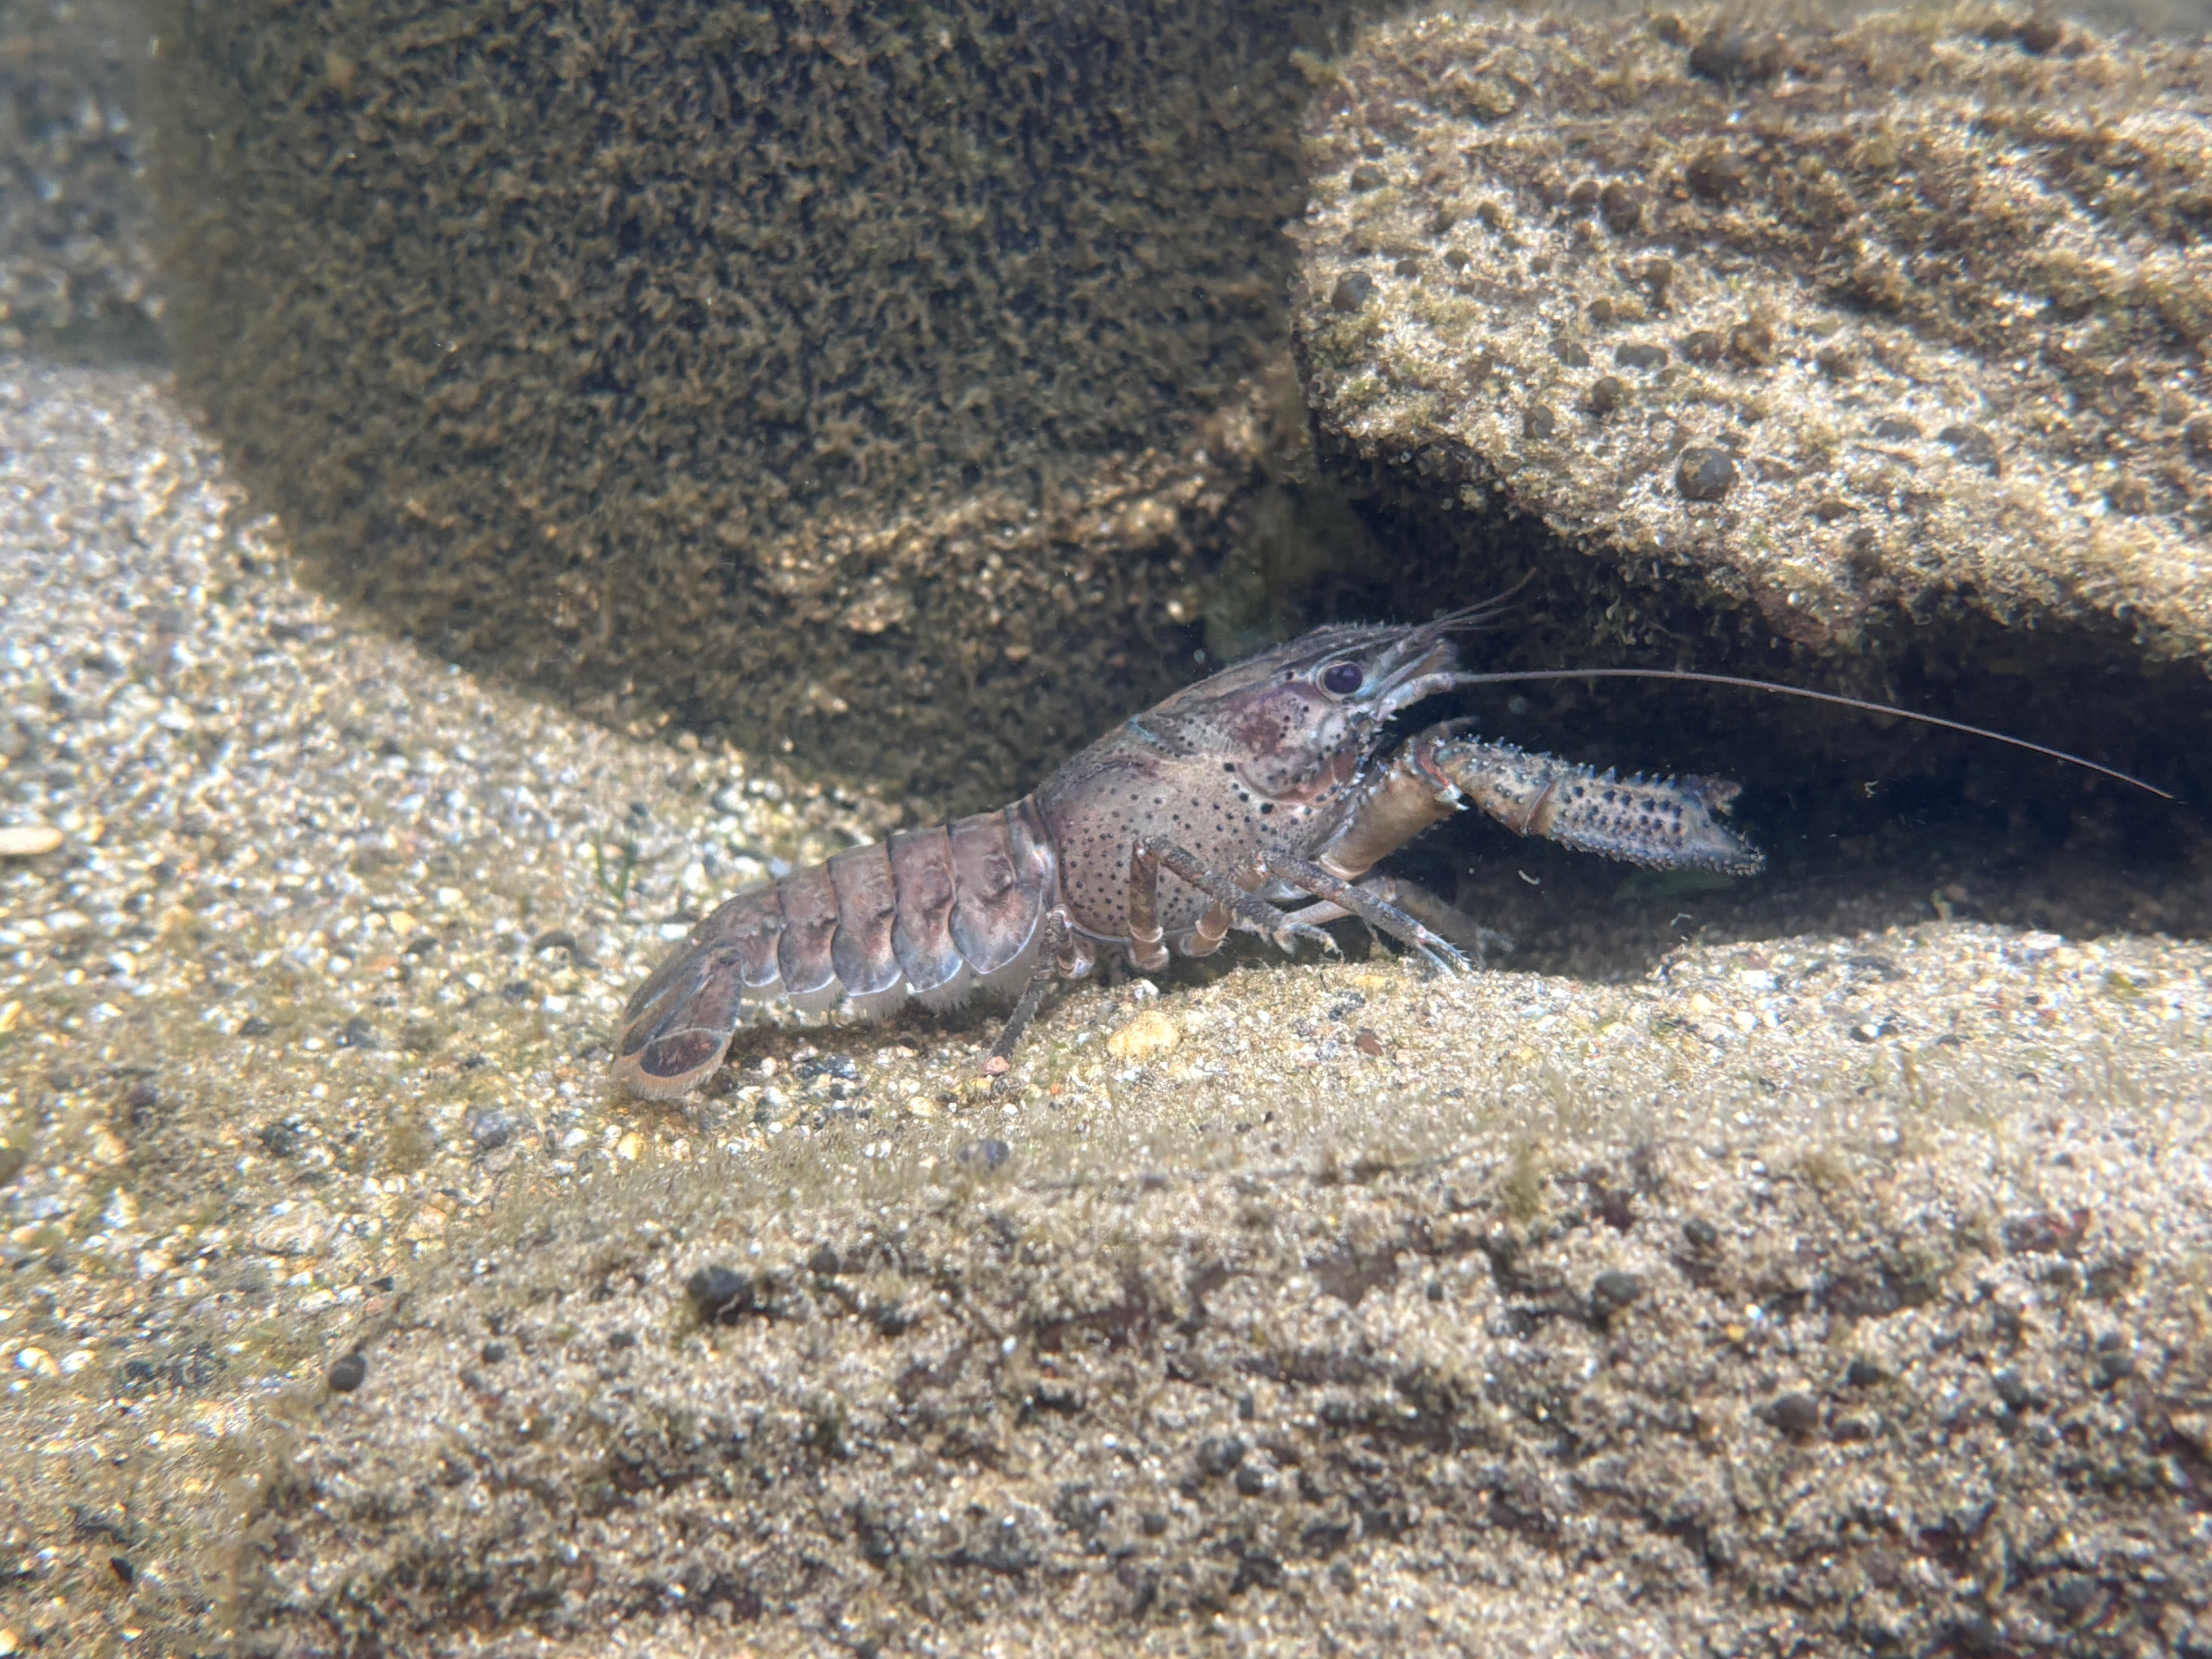
\includegraphics[width=\paperwidth]{images/thesis_cover.jpg}};
  \end{scope}
  \node[color=white, text width=0.92\paperwidth, align=center,
        font=\fontsize{28}{36}\selectfont\bfseries\sffamily]
    at ([yshift=-3cm]current page.north)
    {\hyphenpenalty=10000\exhyphenpenalty=10000 Enhancing native freshwater crayfish habitat in invaded lake ecosystems};
  \node[color=white, align=center,
        font=\fontsize{16}{22}\selectfont\sffamily]
    at ([yshift=4cm]current page.south)
    {Olivier V.\ Raven \\ 2026};
\end{tikzpicture}
\setcounter{chapter}{0}
\null
\clearpage
\thispagestyle{empty}

\frontmatter
\thispagestyle{empty}
\begin{tikzpicture}[remember picture, overlay]
  \draw[line width=0.7pt]
    ([xshift=1.3cm, yshift=-1.3cm]current page.north west)
    rectangle
    ([xshift=-1.3cm, yshift=1.3cm]current page.south east);
\end{tikzpicture}
\vspace*{1.5cm}
\begin{center}

{\fontsize{20}{26}\selectfont\bfseries Enhancing native freshwater crayfish habitat\\[0.3cm]in invaded lake ecosystems}

\vfill

{\fontsize{11}{19}\selectfont
A thesis submitted in partial fulfilment of the requirements\\[0.3cm]
for the degree of\\[0.5cm]
\textbf{Doctor of Philosophy}\\[0.2cm]
Te Aka Mātuatua --- School of Science\\[0.5cm]
at\\[0.5cm]
\textbf{The University of Waikato}\\[0.3cm]
by\\[0.3cm]
\textbf{Olivier V. Raven}
}

\vfill


\includegraphics[width=4.5cm]{images/Waikato_logo.png}

\vspace{0.8cm}

{\fontsize{11}{14}\selectfont 2026}

\end{center}
\vspace*{1.5cm}
\newpage

\clearpage
\thispagestyle{empty}
\begin{minipage}[t][0.96\textheight][s]{\textwidth}

\vspace{0.6cm}

{\fontsize{16}{20}\selectfont\sffamily\bfseries Propositions}

\vspace{0.5cm}
{\color{thesissand}\rule{\textwidth}{1.5pt}}
\vspace{0.6cm}

\begin{enumerate}[label={\bfseries\arabic*.}]
  \setlength{\itemsep}{1.2em}

  \item Structural complexity is essential for the recovery of kōura populations, when
        threatened by non native predator.\\
        \hspace*{1em}{\small\itshape (this thesis)}

  \item The fear of predators shapes prey behaviour as powerfully as predation
        itself, yet invasion biology rarely accounts for it.\\
        \hspace*{1em}{\small\itshape (this thesis)}

  \item Rock pile deployment is a viable and scalable tool for freshwater crayfish
        restoration in lakes, but success depends on location and design, not just presence.\\
        \hspace*{1em}{\small\itshape (this thesis)}

  \item Freshwater crayfish play crucial roles in aquatic ecosystems but are often overlooked.

  \item The current methods of publishing and reviewing scientific research are locked 
        into historical practices that are no longer suitable for today's world.

  \item Scientific knowledge is a public good. It should be openly accessible,
        transparently evaluated, and preserved in a way that keeps it useful and verifiable
        not just today, but across generations.

\end{enumerate}

\vfill

{\color{thesissand}\rule{\textwidth}{0.8pt}}
\vspace{0.4cm}

{\small\sffamily
Propositions belonging to the thesis, entitled\\[0.3em]
\textit{Enhancing native freshwater crayfish habitat in invaded lake ecosystems}\\[0.3em]
Olivier V. Raven\\
The University of Waikato, 2026
}

\end{minipage}
\clearpage

\chapter*{Abstract}\label{abstract}
\addcontentsline{toc}{chapter}{Abstract}

Native freshwater crayfish (\emph{Paranephrops planifrons}, kōura) are a
taonga (treasured) species in Aotearoa New Zealand with a rich history
of harvest and trade by iwi (Māori communities). Over the past two
decades, however, kōura populations have declined by up to 90 \% in Lake
Rotoiti (North Island, New Zealand), making traditional harvesting
unviable. This decline is driven by degraded water quality, intensified
lake stratification, and the spread of invasive fish and macrophytes.
Since around 2016, the non-native brown bullhead catfish (\emph{Ameiurus
nebulosus}) has become established in the lake and preys on kōura,
compounding the effects of other stressors. The decline in kōura,
coupled with multiple threats, indicates that improving habitat is
necessary for kōura population recovery. I hypothesised that habitat
complexity is a key factor moderating predator-prey interactions, thus
helping to prevent predation by non-native catfish, and that habitat
enhancement interventions that increase rocky habitat would have
positive impacts on kōura.

I conducted four complementary studies to investigate potential habitat
enhancement tools: a behavioural controlled laboratory experiment
examining refuge use in response to native and novel predators, a
multi-lake field survey of shoreline habitat associations, a mesocosm
study testing habitat structure configurations and materials, and a
field deployment of stone pile habitats in Lake Rotoiti.

The results of the \textbf{laboratory experiment} revealed that kōura
showed greater refuge use in the presence of the novel catfish than when
exposed to the native predator, longfin eel (\emph{Anguilla
dieffenbachii}), highlighting the importance of refuge on predator-prey
interactions.

The \textbf{field survey} assessed habitat conditions in five lakes
using a structured study design and showed that complex shoreline
habitats consisting of rocks and riparian vegetation were best
predictors of kōura presence. This result helped establish the
importance of rock habitat for extant kōura populations.

The \textbf{mesocosm experiment} evaluated the preference of kōura for
materials that could be used to enhance their habitat. When hole sizes
in habitat elements were held constant, kōura showed no preference
between wood or stone, but more stable, heavier structures were
preferred, and habitat configurations providing refuge heterogeneity
showed broadest appeal across different size classes of kōura.

To evaluate the effects of adding rocky habitat in the littoral zones, I
conducted a \textbf{field experiment} by placing stone piles at five
separate locations in Lake Rotoiti. The study used a quasi-BACI design,
collecting before-and-after data from control, addition and reference
sites. The stone piles attracted kōura at densities similar to those in
natural rocky habitat, demonstrating their potential to support kōura
recovery. However, differences relative to bare control sites did not
reach statistical significance after 18 months. A simulation-based power
analysis suggested that longer monitoring periods are needed to detect
population-level responses.

Together, these findings suggest that habitat complexity is a critical,
actionable lever for kōura conservation, and that stone pile deployment
offers a scalable, low-cost tool for restoring populations in degraded
lake littoral zones. Beyond ecological value, these results provide
practical evidence for restoration efforts that support kōura recovery,
helping restore the traditional practices they have sustained for
generations.

\chapter*{Acknowledgements}\label{acknowledgements}
\addcontentsline{toc}{chapter}{Acknowledgements}

\begin{quote}
``The more we learn, the easier the human world becomes---but the
natural world only grows more wondrous in its complexity''
\end{quote}

First, I would like to express my deepest gratitude to the kōura
(freshwater crayfish) and the giants on whose shoulders I stood to
advance the study of kōura in Aotearoa New Zealand. In particular, I
thank Alan Devcich, C. L. Hopkins, John Quinn, Stephanie Parkyn, Ian
Kusabs, Brendan Hicks, John Hollows, Laura Francis, Grant Barnes, Ian
Jowett, Karin Olsson, Per Nyström, Nisikawa Usio, Colin Townsend, and
many others whose foundational work has shaped our understanding of this
species. It has been a privilege to build upon their contributions and
contribute to the conservation of kōura.

I am profoundly thankful to my supervisors, Deniz Özkundakci, Frank
Burdon, Ian Kusabs, and Robin Holmes for their mentorship, quick
reviewing processes, and unwavering support throughout this PhD journey.
I also extend my appreciation to co-authors, Calum MacNeil and Finnbar
Lee, for their collaboration and insights. This research would not have
been possible without the support and collaboration of Te Arawa Lakes
Trust and Te Komiti Whakahaere. I am especially grateful to Nicki
Douglas, Soweeta Fort-D'ath, William Anaru (Te Arawa Lakes Trust), and
Tihini Grant (Ngāti Pikiao)

My sincere thanks also extend to the Tāheke Opatia Marae, Te Takinga
Marae, and landowners, Meryl Levon, Piripi Curtis, David McIlraith, Piki
Thomas, Haddon Lock, Barnett Vercoe, Richard Vercoe, and Caroline
Newton, for granting access to monitoring sites and facilitating
fieldwork in Lake Rotoiti.

This research was made possible through funding from the Cawthron
Institute's Fish Futures programme, supported by a Ministry of Business,
Innovation and Employment grant (CAWX2101). Thanks to Joanne Clapcott
for incorporating this study into the Fish Futures programme, and to Ian
Kusabs, who initiated the study and obtained the necessary iwi approvals
and regional council consents that enabled the research to proceed.
Additional funding was provided from the Bay of Plenty Regional Council
under the Toihuarewa Waimāori - Bay of Plenty Regional Council Chair in
Lake and Freshwater Science programme. I also acknowledge the
contributions of Andy Bruere (BOPRC), Brendon Cappely (Greenfield
Services Ltd), Joe Butterworth (JFB Enviro Ltd.), Cory O'Neill (Te Arawa
Lakes Trust), Alex Simes (Te Arawa Lakes Trust), Martin Sarkezi (UoW),
Mael Marguet (UoW), Ethan Morgan (UoW), Logan Kallam (UoW), Savio Dsouza
(UoW), and Matt Prentice (UoW), whose assistance with fieldwork, data
collection, and logistical support was indispensable. Special thanks to
Dion and Josh for their friendship and help in constructing wood splits
and blocks.

During my PhD, I became increasingly aware of the limitations of the
current scientific publishing system, with paywalls restricting access,
and a general lack of transparency in how research is evaluated and
cited. This conviction that science should be open, accessible, and
collaborative led me to found ScienceEcosystem.org, an open science
platform working to lower barriers to knowledge sharing. I remain
committed to developing it further in service of that goal.

\subsection*{Use of Artificial
Intelligence}\label{use-of-artificial-intelligence}
\addcontentsline{toc}{subsection}{Use of Artificial Intelligence}

Generative AI (Claude by Anthropic, primarily Sonnet models) was used
during this research for the purpose of assistance with development of R
code for data processing, analysis, and visualisation, with inputs
including data structures, analysis objectives, and existing code. It
also assisted by proof-reading of written sections, with inputs being
draft text authored by the researcher. Code outputs were reviewed and
validated against expected outputs and independently verified results.
Writing suggestions were limited to grammar, sentence structure, and
clarity, and were accepted or rejected at the author's discretion; no
text was generated by or copied from the tool. All analytical decisions,
interpretations, and conclusions are the author's own.

\clearpage
\tableofcontents
\clearpage
\mainmatter

\clearpage
\providecommand{\chaptermark}[1]{}
\ifcsname c@chapter\endcsname
\setcounter{chapter}{1}
\setcounter{figure}{0}
\setcounter{table}{0}
\setcounter{section}{0}
\addcontentsline{toc}{chapter}{\protect\numberline{1}General Introduction}
\chaptermark{General Introduction}
\fi
\providecommand{\thechapter}{1}
\thispagestyle{empty}
\begin{tikzpicture}[remember picture, overlay]
  \node[inner sep=0pt] at ([yshift=-3.5cm]current page.center)
    {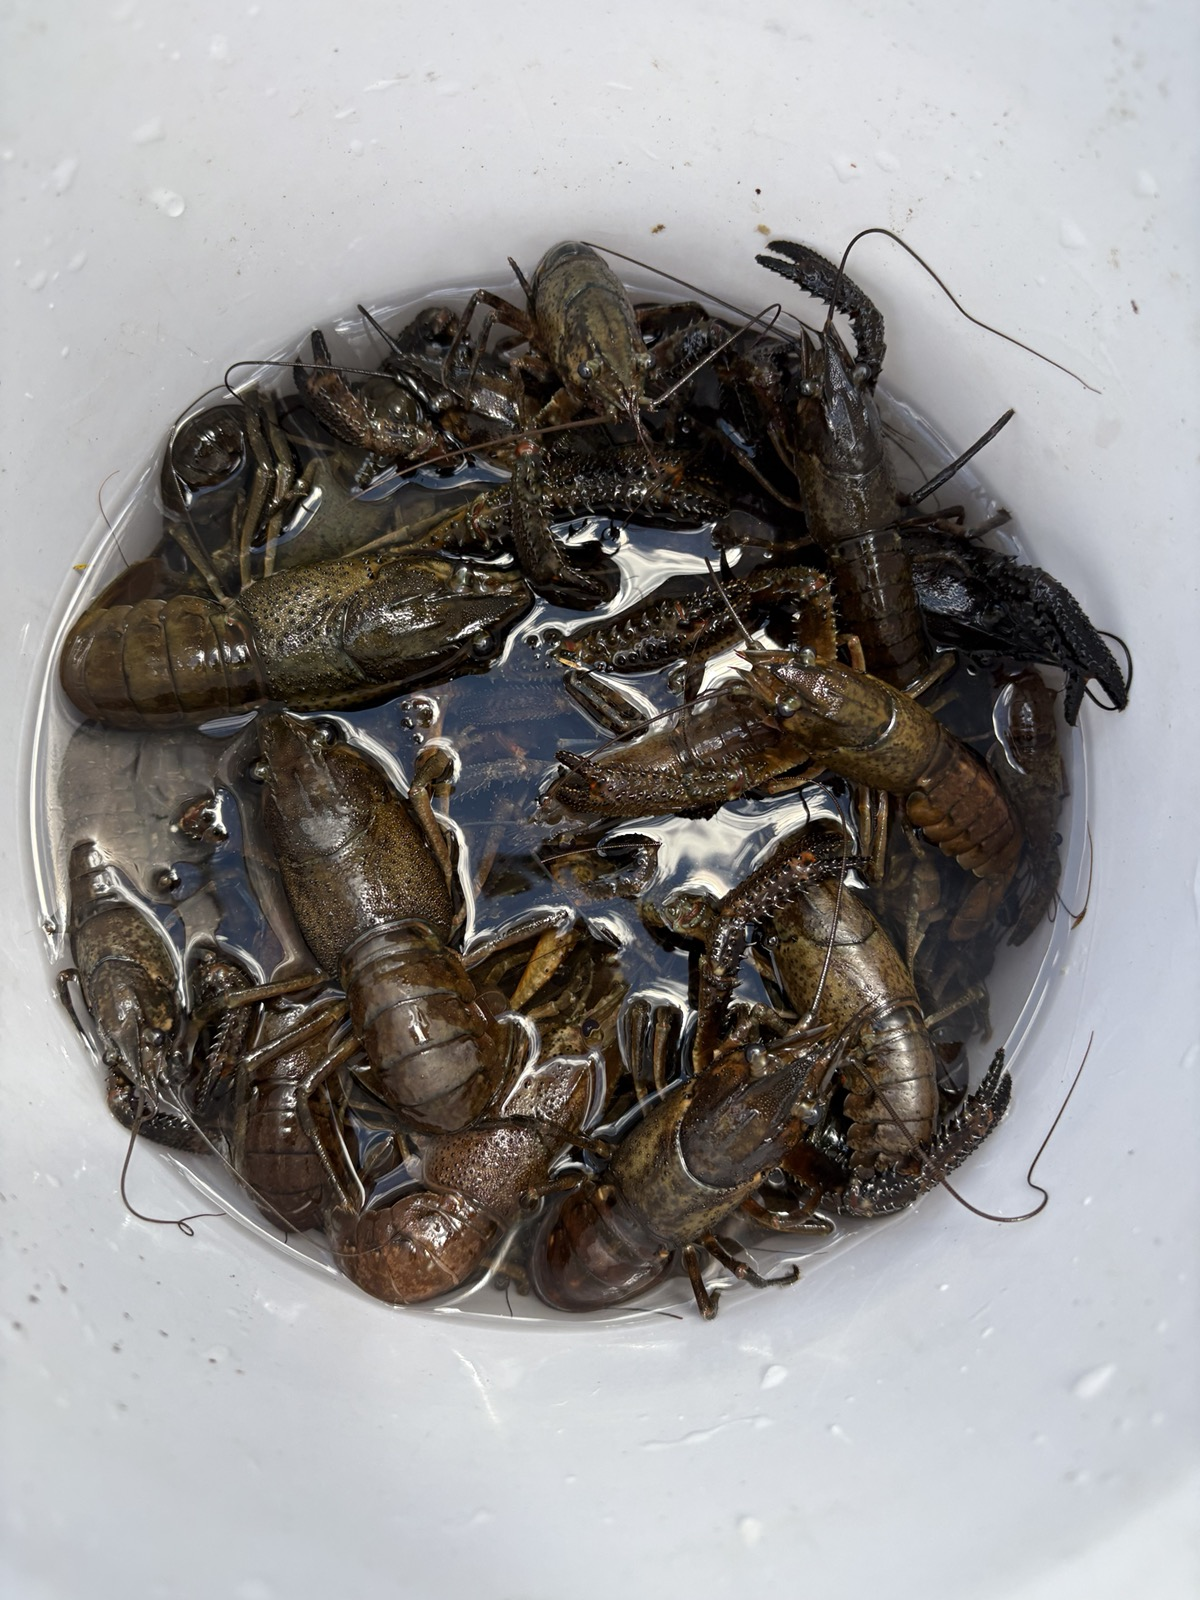
\includegraphics[width=\paperwidth,height=\paperheight]{images/ch1_cover.jpg}};
  \fill[black]
    (current page.north west) rectangle ([yshift=-7cm]current page.north east);
  \node[color=thesissand, align=left,
        font=\fontsize{13}{16}\selectfont\sffamily, anchor=west]
    at ([xshift=1.5cm, yshift=-1.5cm]current page.north west)
    {Chapter \thechapter};
  \node[color=white, text width=0.85\paperwidth, align=left,
        font=\fontsize{22}{28}\selectfont\bfseries\sffamily, anchor=west]
    at ([xshift=1.5cm, yshift=-4cm]current page.north west)
    {General Introduction};
\end{tikzpicture}
\null
\clearpage

\section{Global freshwater ecosystem
decline}\label{global-freshwater-ecosystem-decline}

Ecosystems worldwide are increasingly impacted by drivers of global
change, with freshwater environments amongst the most degraded
particularly from land-use activities, introduced species, and climate
change (Harrison et al. 2018). This degradation is particularly
concerning given that freshwater systems disproportionately support
biodiversity and ecosystem services relative to their global area
(Dudgeon et al. 2006). Among freshwater ecosystems, lakes are
particularly sensitive to land-use pressures because they integrate
inputs from their entire catchment, accumulating nutrients, sediment,
and contaminants over time (Bhateria and Jain 2016).

Within lakes, the shallow littoral zone which is the productive
interface between the terrestrial and aquatic system where stressors
coverage most acutely (Strayer and Findlay 2010). Exposure to sunlight,
enables photosynthesis in plants and algae, making the littoral zone one
of the most productive and biodiverse areas in lakes (Vadeboncoeur et
al. 2011; Geist and Hawkins 2016; Porst et al. 2019). In its shallow
regions, emergent vegetation flourishes, creating essential nurseries
for numerous species (Meerhoff and González-Sagrario 2022) and
contributing significantly to the energy and nutrient cycling within
lake food webs. Structurally complex areas in the littoral zone,
including rocky habitats, can function as refugia, buffering multiple
species against co-occurring threats, making their protection a
conservation priority (Selwood and Zimmer 2020).

Despite this ecological importance, lake shorelines are often heavily
impacted by human activities such as hardening, the introduction of
invasive species, and pollution (Vadeboncoeur et al. 2002; Strayer and
Findlay 2010). The effects of eutrophication and predation by non-native
species in the littoral zone remain relatively understudied (Vander
Zanden and Vadeboncoeur 2020). Reversing this degradation requires
targeted interventions, which are often complex and resource-intensive
(Palmer et al. 2005). This challenge has nonetheless driven recent
global commitments to ecosystem restoration, including the reduction of
nutrient inputs through buffer zones at lakes inlets and the
rehabilitation of landscape connectivity (Meerhoff et al. 2022).

\section{Ecosystem and habitat
restoration}\label{ecosystem-and-habitat-restoration}

Reversing widespread degradation of freshwater ecosystems, has prompted
growing global investment in ecosystem and habitat restoration. The UN
declared 2020-2030 the Decade for Ecosystem Restoration, with the goal
of halting the degradation of ecosystems worldwide and made specific
resolutions on sustainable lake management (UN. General Assembly 2019;
Gann et al. 2019; United Nations Environment Programme 2022; Cooke et
al. 2022). This commitment reflects a broader conservation imperative,
as habitat degradation and loss remain key drivers of regional
population extinction (Heinrichs et al. 2016).

Ecosystem restoration aims to recover an entire ecosystem, including its
structure, function and dynamics, often with the goal of enhancing
resilience to future stressors (Palmer and Ruhl 2015). Habitat
restoration is a more targeted component of this broader goal, focusing
on enhancing the quality or availability of habitat for a specific
species or community, rather than an entire ecosystem (Miller and Hobbs
2007). Approaches to habitat restoration across terrestrial, coastal,
and freshwater systems vary widely depending on the system and species
involved, but commonly include replanting native vegetation, removing
barriers like dams, or adding complexity to a habitat that has become
simplified or degraded (Banks-Leite et al. 2020; Loch et al. 2020). The
deliberate addition of hard substrate, such as boulders, large wood,
gravel, or habitat unites, is one of the more direct and widely applied
forms of habitat restoration, since many species depend on physical
complexity for shelter, feeding or reproduction (Geist and Hawkins
2016).

Restoring structural complexity is comparatively well-established in
marine systems, where artificial reefs are placed on the seafloor to
rebuild complexity lost from degraded or removed natural reef habitat
like coral and oyster reefs (Yanovski and Abelson 2019;
Esquivel-Muelbert et al. 2026), supporting biodiversity recovery and
fisheries productivity (Frehse et al. 2025). While artificial reefs are
most often associated with marine environments, the same principle that
adding physical structure to a degraded habitat can restore the
complexity and shelter availability, extends to freshwater systems as
well, including lentic environments such as lakes, where littoral zone
habitat restoration remains comparatively underdeveloped (Geist and
Hawkins 2016).

In freshwater environments, habitat restoration has been applied through
the addition of habitat enhancement structures like, rocks, woody
debris, or other natural substrates to streams and lakes that have lost
structural complexity through historic modification, sedimentation, or
substrate removal (Smokorowski and Pratt 2007; Roni et al. 2008; Parkyn
et al. 2009). These additions have been used to support a range of
freshwater taxa, including fish and invertebrates, by recreating the
kind of structurally complex habitats that naturally support shelter,
feeding and reproduction (Santos et al. 2011; McLean et al. 2015; Zhu et
al. 2021). However, not all added structures achieve their intended
benefit. Poorly designed or inappropriate materials, such as plastic
habitat structures, can fail to replicate natural habitat function and
risk becoming a form of littering rather than restoration (Baine 2001;
Cooke et al. 2023), underscoring the importance of careful design when
structures are used as a restoration tool. Within freshwater systems,
structural restoration is particularly relevant for taxa that depend on
physical complexity for shelter, including freshwater crayfish, which
are ecologically important but undergoing severe declines globally
(Richman et al. 2015).

\section{Freshwater crayfish: ecology and global
decline}\label{freshwater-crayfish-ecology-and-global-decline}

Freshwater crayfish are decapod crustaceans that form an important
component of benthic macroinvertebrate communities in a wide range of
freshwater ecosystems. They belong to the infraorder Astacidea, which is
divided into two superfamilies: Astacoidea, restricted to the Northern
Hemisphere, and Parastacoidea, restricted to the Southern Hemisphere
(Crandall and De Grave 2017). The Astacoidea contains three families,
Astacidae (western Eurasia and western North America), Cambaridae
(eastern North America), and Cambaroididae (eastern Asia), while the
Parastacoidea contains a single family, Parastacidae, with 15 genera
distributed across Australia, New Zealand, New Guinea, South America,
and Madagascar (Figure~\ref{fig-crayfish-families}) (Crandall and De
Grave 2017). Crayfish have a segmented exoskeleton with chelipeds
(pincers) used for foraging, defence, and manipulating their
environment. They are omnivorous, functioning as scavengers, predators,
and prey within freshwater food webs (Momot 1995; Reynolds et al. 2013).
Through burrowing, bioturbation, sediment reworking, macrophyte
consumption, and the processing of organic matter, crayfish exert
disproportionate effects on freshwater ecosystems (Nyström et al. 1996;
Statzner et al. 2003; Creed and Reed 2004), making them important
ecosystem engineers and keystone species (Crandall and Buhay 2008; Jones
et al. 2016).

Despite their significant ecological role, 32 \% of crayfish species
worldwide are threatened with extinction (Richman et al. 2015) due to
numerous threats, including habitat degradation, pollution, invasive
species, and overexploitation. Among these invasive species, are a
particularly pervasive and difficult to manage threat, as non-native
fish and crayfish can, prey on native species, compete for habitat, and
spread diseases (Danilović et al. 2022). For example, in Europe native
crayfish such as \emph{Astacus astacus}, \emph{Austropotamobius
pallipes}, and \emph{A. torrentium} are threatened by the crayfish
plague pathogen (\emph{Aphanomyces astaci}, an oomycete), which is
carried asymptomatically by many North American crayfish species
(Holdich et al. 2009). These combined pressures mean that conservation
of native crayfish requires not only an understanding of the threats
they face, but also of the habitats they depend on, a challenge
particularly acute for endemic species in geographically isolated
systems such as those of Aotearoa New Zealand.

\begin{figure}

\centering{

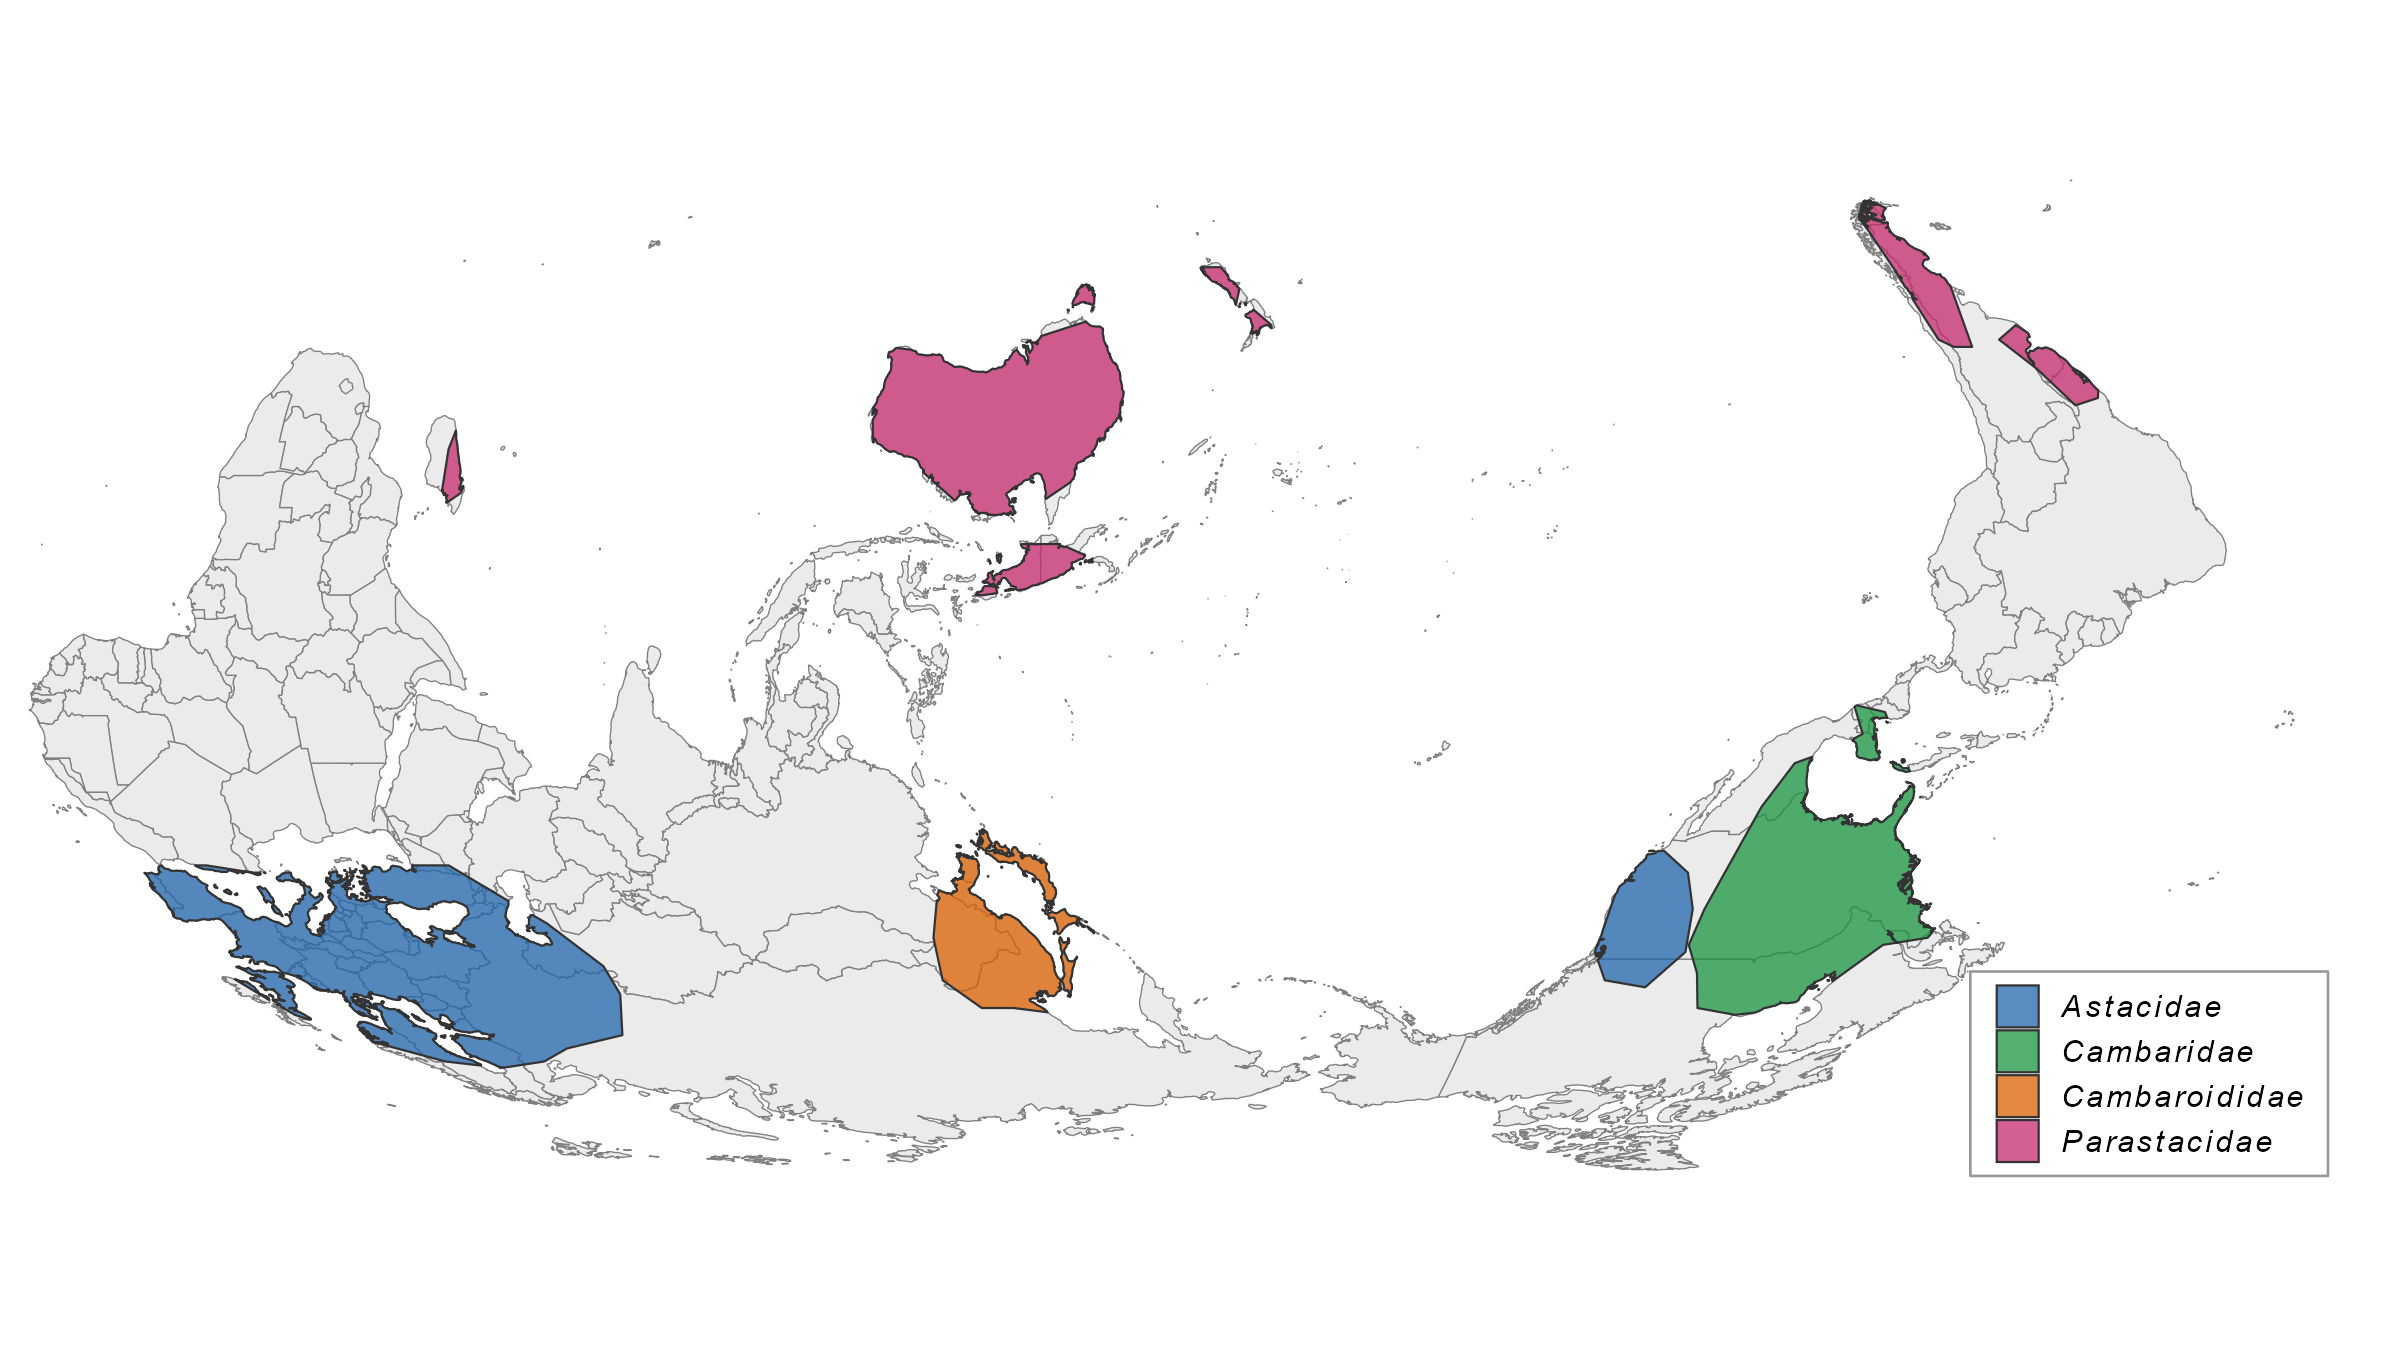
\includegraphics[width=0.65\linewidth,height=\textheight,keepaspectratio]{images/fig-crayfish-families.png}

}

\caption{\label{fig-crayfish-families}Global native distribution of
freshwater crayfish families, following Crandall and De Grave (2017).
Adapted from: (Fetzner 2019).}

\end{figure}%

\section{Kōura: Aotearoa's native freshwater
crayfish}\label{kux14dura-aotearoas-native-freshwater-crayfish}

Aotearoa New Zealand's (hereafter Aotearoa) native biota is
disproportionately made up of endemic species because of its island
biogeography and isolated location (Wallis and Trewick 2009). The two
endemic species of freshwater crayfish found in Aotearoa are of the
genus \emph{Paranephrops}. These freshwater crayfish are also known by
the Māori name kōura, although some iwi (Māori tribal groups) use other
names including kēwai, kēkēwai, and koeke (Kusabs et al. 2018). The two
species are the northern kōura (\emph{Paranephrops planifrons} White,
1842) and the southern kōura (\emph{P. zealandicus} {[}White, 1847{]}).
The northern kōura can be found throughout the North Island and on the
west side of the Southern Alps on the South Island
(Figure~\ref{fig-nz-distribution-maps}). The southern kōura can be found
on the eastern and southern part of the South Island and on Stewart
Island.

\begin{figure}

\centering{

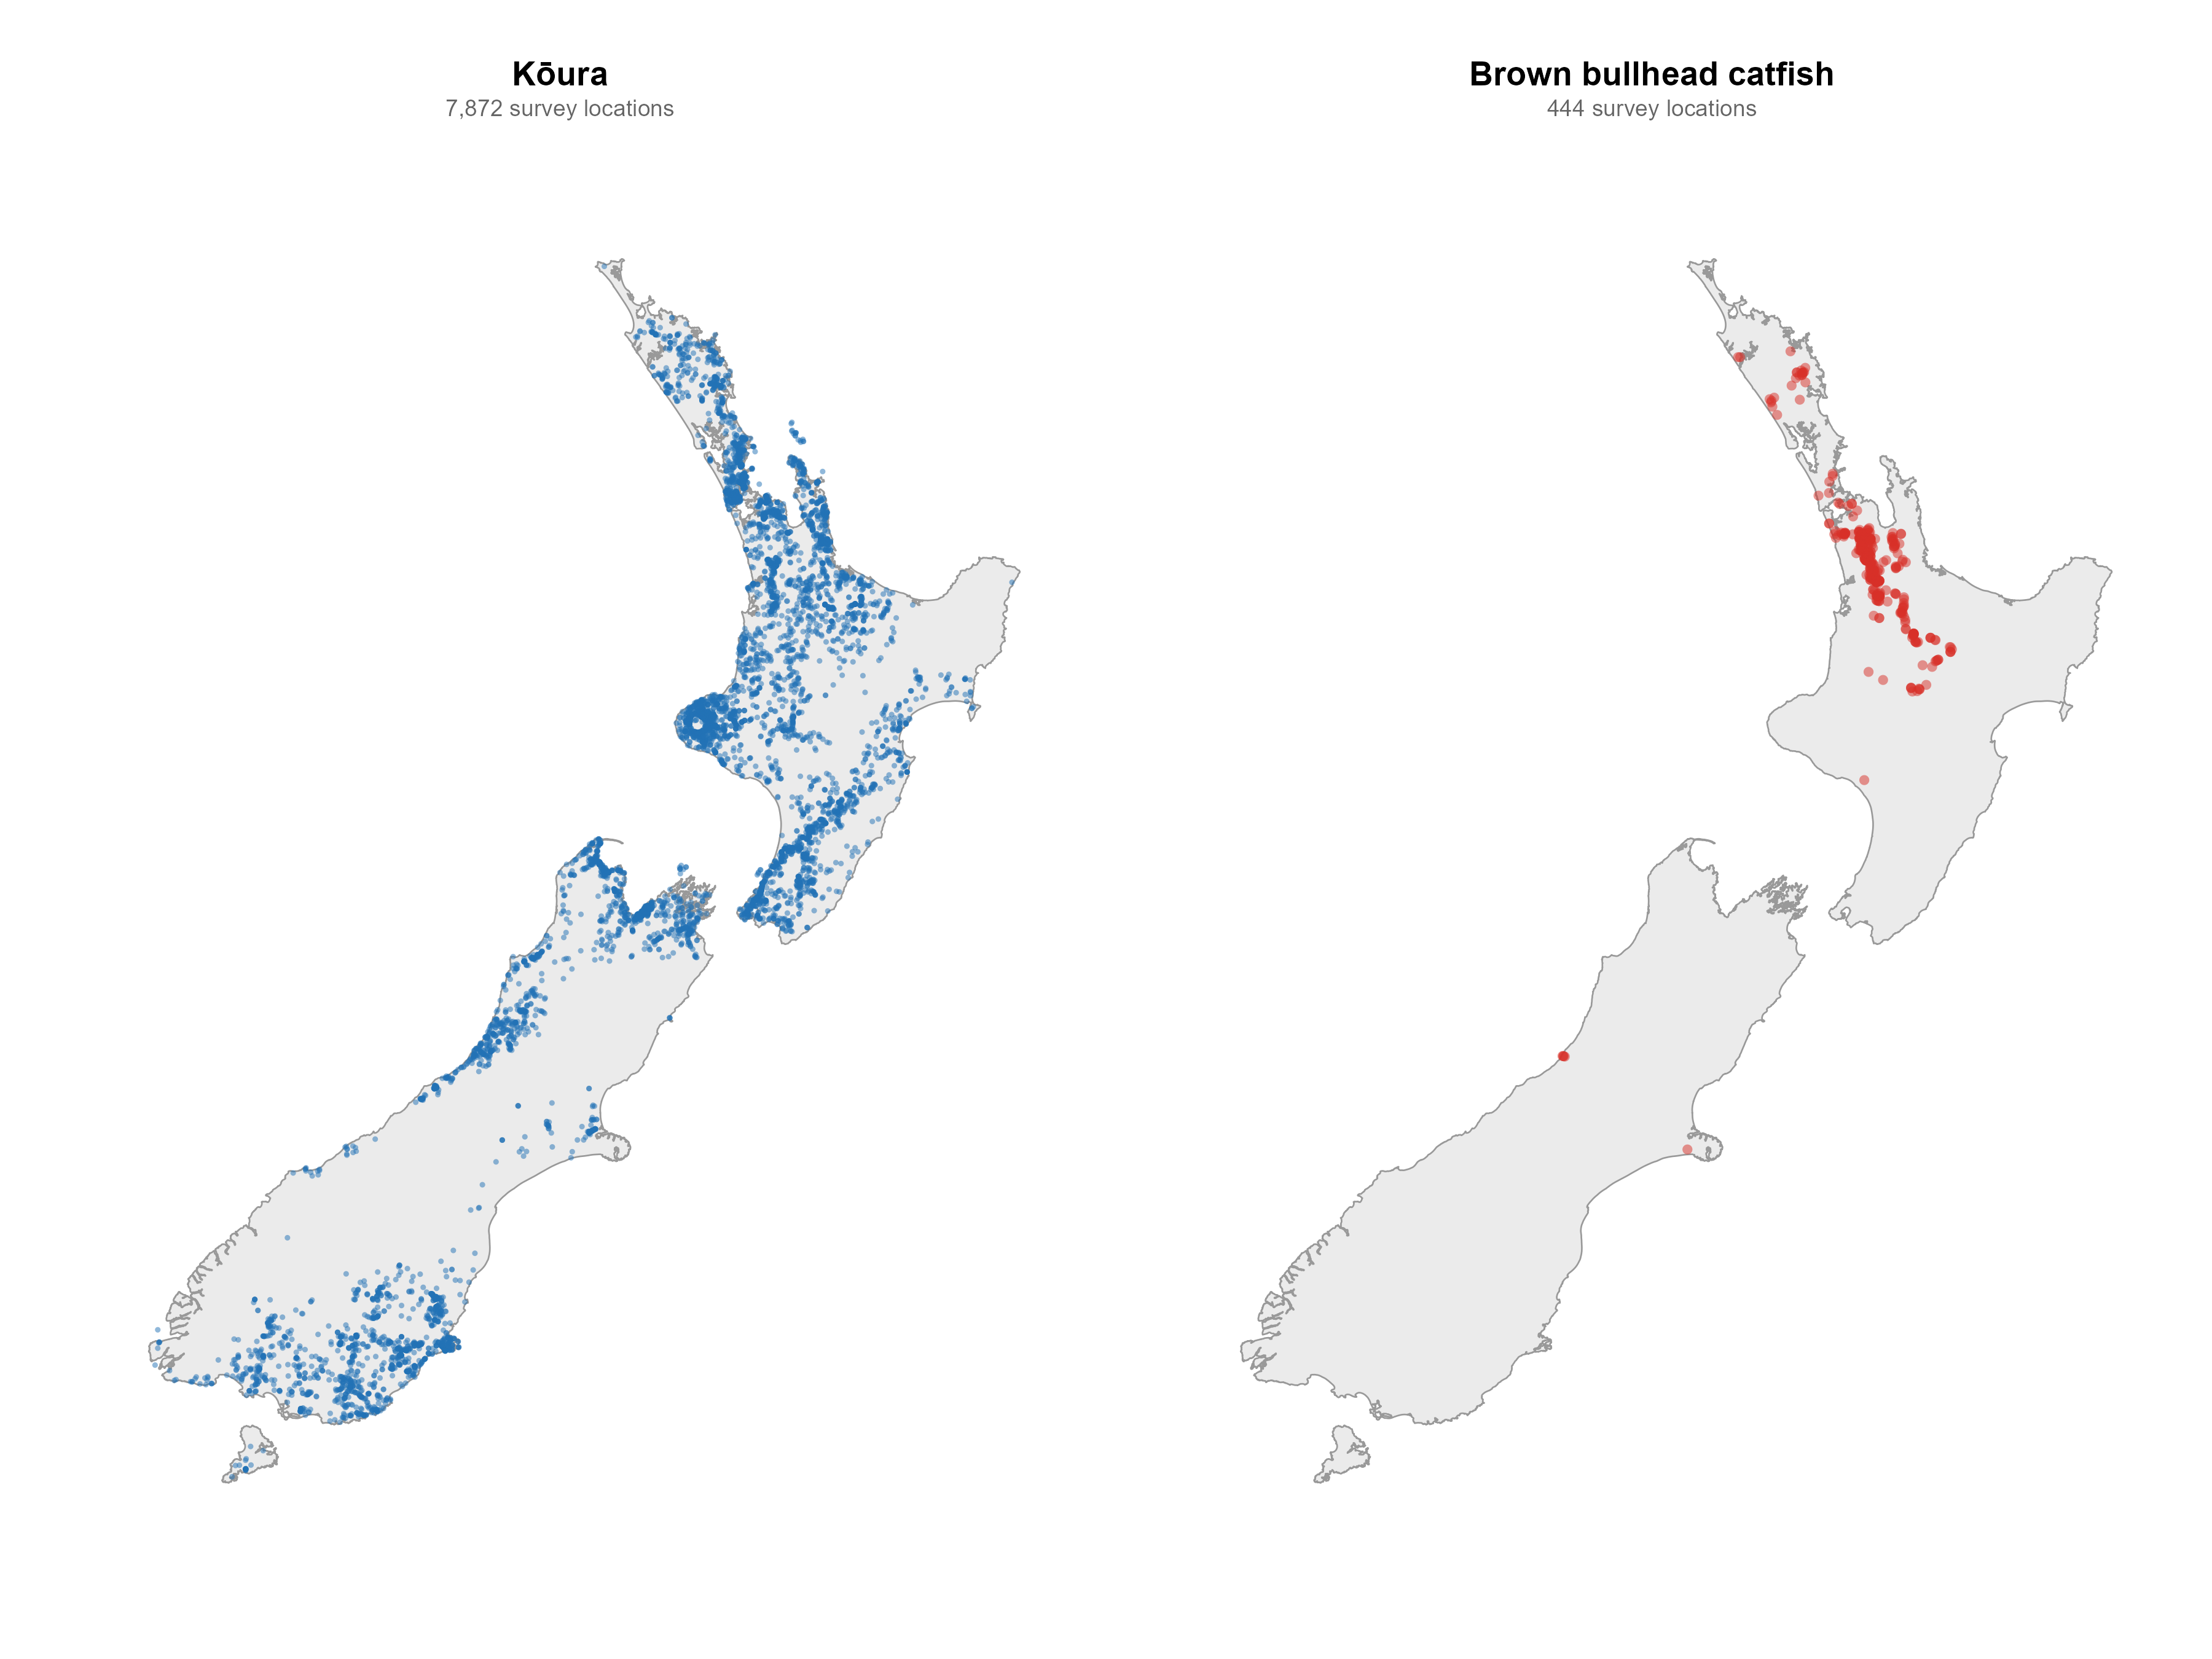
\includegraphics[width=0.65\linewidth,height=\textheight,keepaspectratio]{outputs/fig-nz-distribution-maps.png}

}

\caption{\label{fig-nz-distribution-maps}Distribution of kōura (blue,
left) and brown bullhead catfish (\emph{Ameiurus nebulosus}, red,
right), an introduced predator discussed in the following section, in
Aotearoa New Zealand. Source: New Zealand Freshwater Fish Database
(Stoffels 2024).}

\end{figure}%

\subsection{Biology, ecology, and habitat
use}\label{biology-ecology-and-habitat-use}

Kōura inhabit a range of freshwater environments including streams,
rivers and lakes and have been described as ecosystem engineers and
keystone species in Aotearoa (Collier et al. 1997; Usio and Townsend
2004). They are associated with structurally complex habitats that
provide physical shelter, preferring coarse gravel and rocky substrates
in both streams and lakes (Jowett et al. 2008; Kusabs et al. 2015b). In
streams, the highest abundances have been recorded on substrates with an
average particle size of 130 mm (Olsson 2008; Jowett et al. 2008). Kōura
avoid areas where dissolved oxygen levels drop below 5 mg/L and
temperatures exceed 21 °C (Devcich 1979). Where suitable natural
substrates are rare, kōura can excavate tunnels or burrows to provide
cover, a behaviour documented in Lake Tikitapu, where the bottom
sediment substrate permits burrowing (Pers. Comm. Ian Kusabs).

Kōura are nocturnal, retreating to deeper waters or physical shelters
during the daylight hours to avoid predators, and emerging at night to
forage, with some populations known to move in to the productive shallow
zones of lakes (Devcich 1979). Kōura have direct development, meaning
juveniles hatch as miniature adults with no free-living larval stage.
Females carry eggs and newly hatched juveniles beneath the abdomen for
approximately three weeks before release, typically at depths of less
than 10 m in lakes (Parkyn and Kusabs 2007). Juveniles mature in two to
three years depending on water temperature (Devcich 1979; Parkyn 2000).

\subsection{Cultural significance and population
decline}\label{cultural-significance-and-population-decline}

Kōura continue to be an important food source for Māori and are
considered a taonga (treasured) species (Parkyn and Kusabs 2007; Kusabs
and Quinn 2009; Morris 2024). Māori harvest kōura alongside other kai
(food) in specific periods of the year according to Maramataka (the
Māori lunar calendar) (Hiroa 1921; Henare 2008). For kōura, this period
is from beginning of kōanga (spring) until halfway through ngahuru
(autumn). Kōura are traditionally harvested using baited traps,
handpicking, or the tau kōura which uses several whakaweku (fern
bundles) attached to a tāuhu by pekapeka (Figure~\ref{fig-tau-koura})
(Parkyn and Kusabs 2007; Kusabs and Quinn 2009). In the Rotorua Te Arawa
Lakes (a group of twelve volcanic lakes in the central North Island, see
Study system below), kōura fisheries held significant cultural,
economic, and nutritional importance. Historically, kōura were not only
a vital food source but also served as a medium for trade and barter
among the Te Arawa iwi and hapū. The tau kōura is still used today, but
mostly for research and monitoring of kōura abundance in lakes (Kusabs
and Quinn 2009; Kusabs et al. 2018). Kōura monitoring from 2005 to 2025
revealed declines of 76 \% and 91 \% in kōura catch per unit effort
(CPUE) in Lakes Rotorua and Rotoiti respectively
(Figure~\ref{fig-koura-decline}). These declines reflect a
multiple-stressor problem: long-term water quality deterioration and
habitat loss from invasive macrophytes have reduced kōura populations
over decades, with the recent establishment of the brown bullhead
catfish (\emph{Ameiurus nebulosus}) as a novel predator compounding
these pressures and accelerating the decline (Kusabs et al. 2026).

\begin{figure}

\centering{

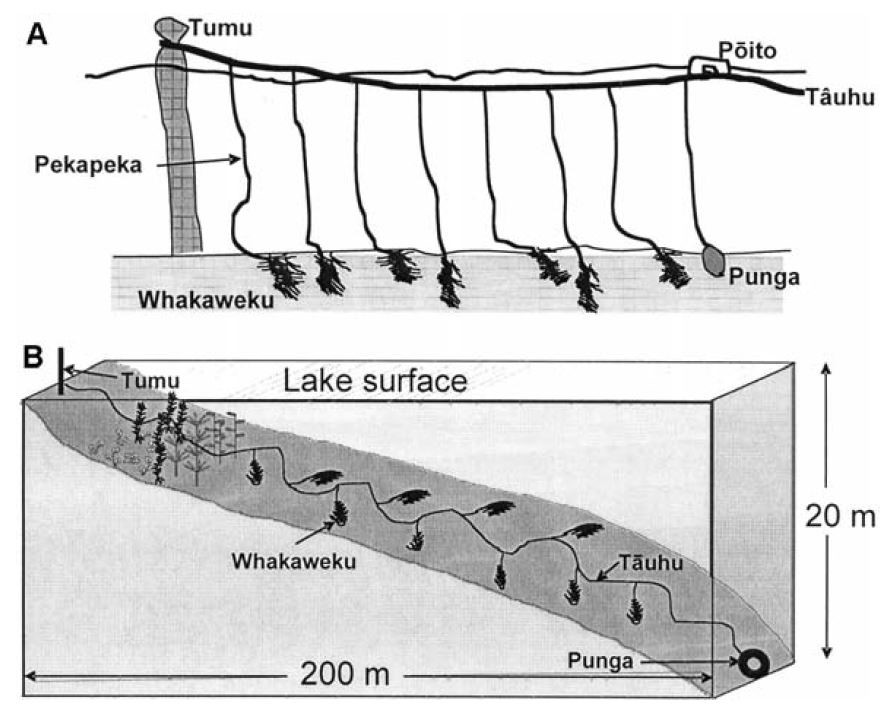
\includegraphics[width=0.65\linewidth,height=\textheight,keepaspectratio]{images/fig-tau-koura.png}

}

\caption{\label{fig-tau-koura}Two versions of the tau kōura as it can be
used for harvesting kōura in a lake. © Copyright Ian Kusabs.}

\end{figure}%

\begin{figure}

\centering{

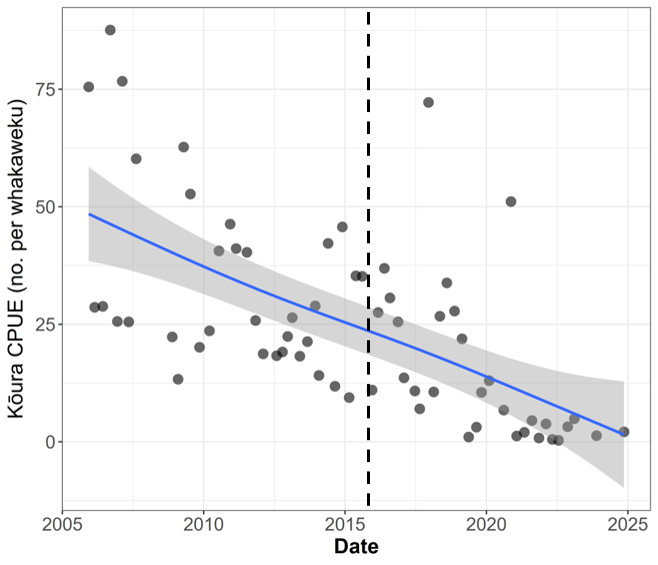
\includegraphics[width=0.65\linewidth,height=\textheight,keepaspectratio]{images/fig-koura-decline2.png}

}

\caption{\label{fig-koura-decline}Kōura catches in CPUE in Lake Rotoiti
at the Ōkere inlet between 2005 and 2024. Kōura were caught using the
tau kōura. The dashed vertical line indicates first confirmed catfish
detection in Lake Rotoiti (2016). Adapted from (Kusabs et al. 2026).}

\end{figure}%

\section{Brown bullhead catfish: a novel predator in Aotearoa
lakes}\label{brown-bullhead-catfish-a-novel-predator-in-aotearoa-lakes}

The brown bullhead catfish (\emph{Ameiurus nebulosus} {[}Lesueur,
1819{]}, hereafter catfish) is native to North America but has been
introduced worldwide for aquaculture and as a game fish, contributing to
profound ecological and economic disruption that biological invasions
cause globally (Haubrock et al. 2025). In Aotearoa, 140 individuals were
introduced in 1877 to Lake St John (Lake Waiatarua) in the Auckland
region, reportedly by mistake, as the intended species was the channel
catfish (\emph{Ictalurus punctatus} (Rafinesque, 1818)) (Barnes 1996).
Although Lake St John has since been drained, catfish persisted and have
spread throughout the upper North Island via accidental and deliberate
releases (Figure~\ref{fig-nz-distribution-maps}). Lake Taupō was first
invaded in 1985 following an illegal release (Barnes 1996). In the
Rotorua Te Arawa Lakes, a dead catfish was found at Okawa Bay in Lake
Rotoiti in 2009 (Blair and Hicks 2009) and sightings followed in 2014,
but surveys failed to detect catfish until 2016, when multiple
individuals were found at the western end of Lake Rotoiti, including Te
Weta Bay where catfish were recovered during macrophyte harvesting
operations (Francis 2019). Catfish subsequently spread to Lake Rotorua
in 2018 via the Ōhau Channel. Since 2016, routine monitoring and active
control fishing have been carried out to reduce their impact (Grayling
2020).

Catfish are physiologically tolerant of a wide range of conditions,
including elevated temperatures and low dissolved oxygen (Scott and
Crossman 1973); this resilience allows them to persist under stressors
that increasingly impact native species (Lee et al. 2025). They are
omnivorous benthic feeders, with individuals reaching 200-455 mm in
length and living up to eight years (Barnes 1996). Their diet overlaps
with, and partly consists of, native species leading to both competition
and direct predation (Figure~\ref{fig-catfish-dissection}) (Scott and
Crossman 1973; Dedual 2019).

Catfish are known predators of kōura and have contributed to declining
kōura CPUE in Lakes Rotorua and Rotoiti (Kusabs et al. 2026). While
kōura abundance had been declining before catfish establishment, the
decline became less variable after 2016, with fewer recovery periods,
suggesting catfish have reduced the population's capacity to rebound
(Kusabs et al. 2026). Catfish habitat use varies seasonally: in lakes,
catfish occupy depths down to approximately 17 m (Dedual 2002) and shift
between weedy and rocky habitats depending on the season, primarily
rocky habitats in winter when macrophytes die back, and both habitat
types during autumn and spring (Barnes 1996; Barnes and Hicks 2003).
Spawning occurs in nests excavated in mud or sand, typically in shallow
areas near rocks or submerged tree trunks for protection (Scott and
Crossman 1973). Nests are roughly the size of the female, who may carry
between 2,000 and 13,000 eggs depending on body size (Scott and Crossman
1973). Acoustic tagging of catfish in Lake Rotoiti confirmed these
seasonal patterns: catfish concentrated in nearshore shallows during
spring and summer, likely seeking warmer water for feeding and
reproduction, before dispersing to mid-water offshore habitats in
winter, consistent with earlier reports of maximum depths around 17 m
(Dedual 2002), rarely exceeding 15 m depth even when the lake is
considerably deeper (Blanchfield et al. 2026).

Critically, Aotearoa lacks native Siluriformes, meaning kōura and other
native fauna have no evolutionary history with catfish and may therefore
fail to recognise them as a predator, a phenomenon termed predator
naiveté (Sih et al. 2010; Carthey and Banks 2014). Predator naiveté can
leave prey populations particularly vulnerable because effective
antipredator responses are often shaped by prior exposure over
evolutionary time (Sih et al. 2010). However, prey may alternatively
respond with generalised fear toward any novel or unfamiliar stimulus,
producing exaggerated antipredator behaviour regardless of actual threat
level (Sih et al. 2023). Beyond direct consumption, predator presence
alone can alter prey behaviour by increasing refuge use, decreasing
movement and suppressing foraging. These non-consumptive effects (NCEs)
can lead to reduced growth and reproduction (Preisser and Bolnick 2008).
The availability of physical refugia is central to mediating these
effects as structurally complex habitats allow prey to shelter from
predation risk while retaining access to foraging opportunities (Selwood
and Zimmer 2020). Restoring structural habitat may therefore buffer the
non-consumptive effects of living alongside a novel predator.

\begin{figure}

\centering{

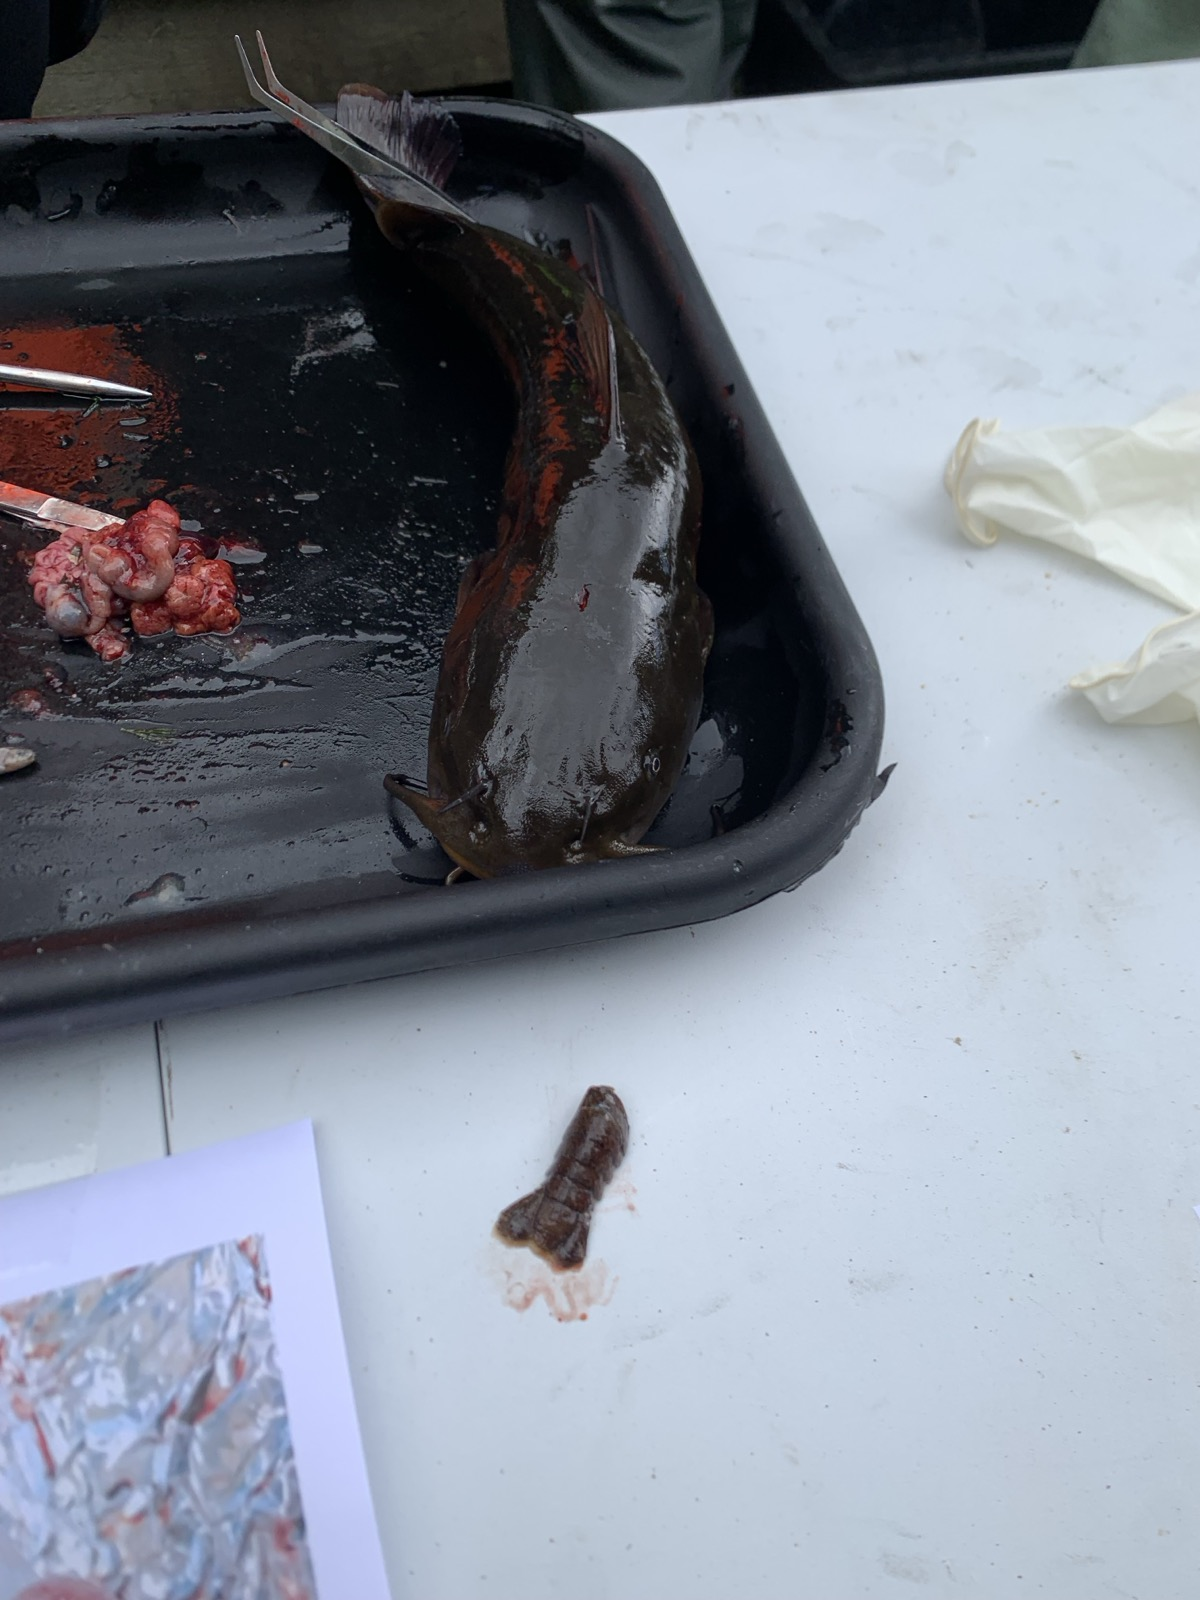
\includegraphics[width=0.65\linewidth,height=\textheight,keepaspectratio]{images/fig-catfish-dissection.png}

}

\caption{\label{fig-catfish-dissection}Dissection of a catfish from Lake
Rotoiti revealed kōura remains (tail) and smelt in its stomach. As smelt
are pelagic and unlikely to be caught by catfish in open water, some
prey items, including potentially the kōura, may have been consumed
while both species were co-trapped in the fyke net rather than through
active predation in the lake.}

\end{figure}%

\section{Study system: the Rotorua Te Arawa
Lakes}\label{study-system-the-rotorua-te-arawa-lakes}

This research was conducted in the Rotorua Te Arawa Lakes, a group of
twelve volcanic lakes in the central North Island of Aotearoa (Bay of
Plenty region; Figure~\ref{fig-study-lakes-map};
Table~\ref{tbl-bop-lake-overview}). The lakes were formed by rhyolitic
volcanic activity over the past \textasciitilde230,000 years and
continue to experience volcanic influence, most recently through the
1886 eruption of Mount Tarawera, which deposited basalt scoria and the
distinctive Rotomāhana Mud across the surrounding catchments (Cole et
al. 2014). The lakes vary considerably in size (0.3--81 km²) and maximum
depth (13.5--125 m), and span a gradient of mixing regimes and trophic
states from oligotrophic (e.g.~Tarawera, Rotomā) to eutrophic
(e.g.~Rotorua, Ōkaro; Table~\ref{tbl-bop-lake-overview}). This diversity
makes the Te Arawa Lakes a particularly informative system for studying
how kōura respond to differing combinations of habitat structure, water
quality, and predator presence.

\begin{figure}

\centering{

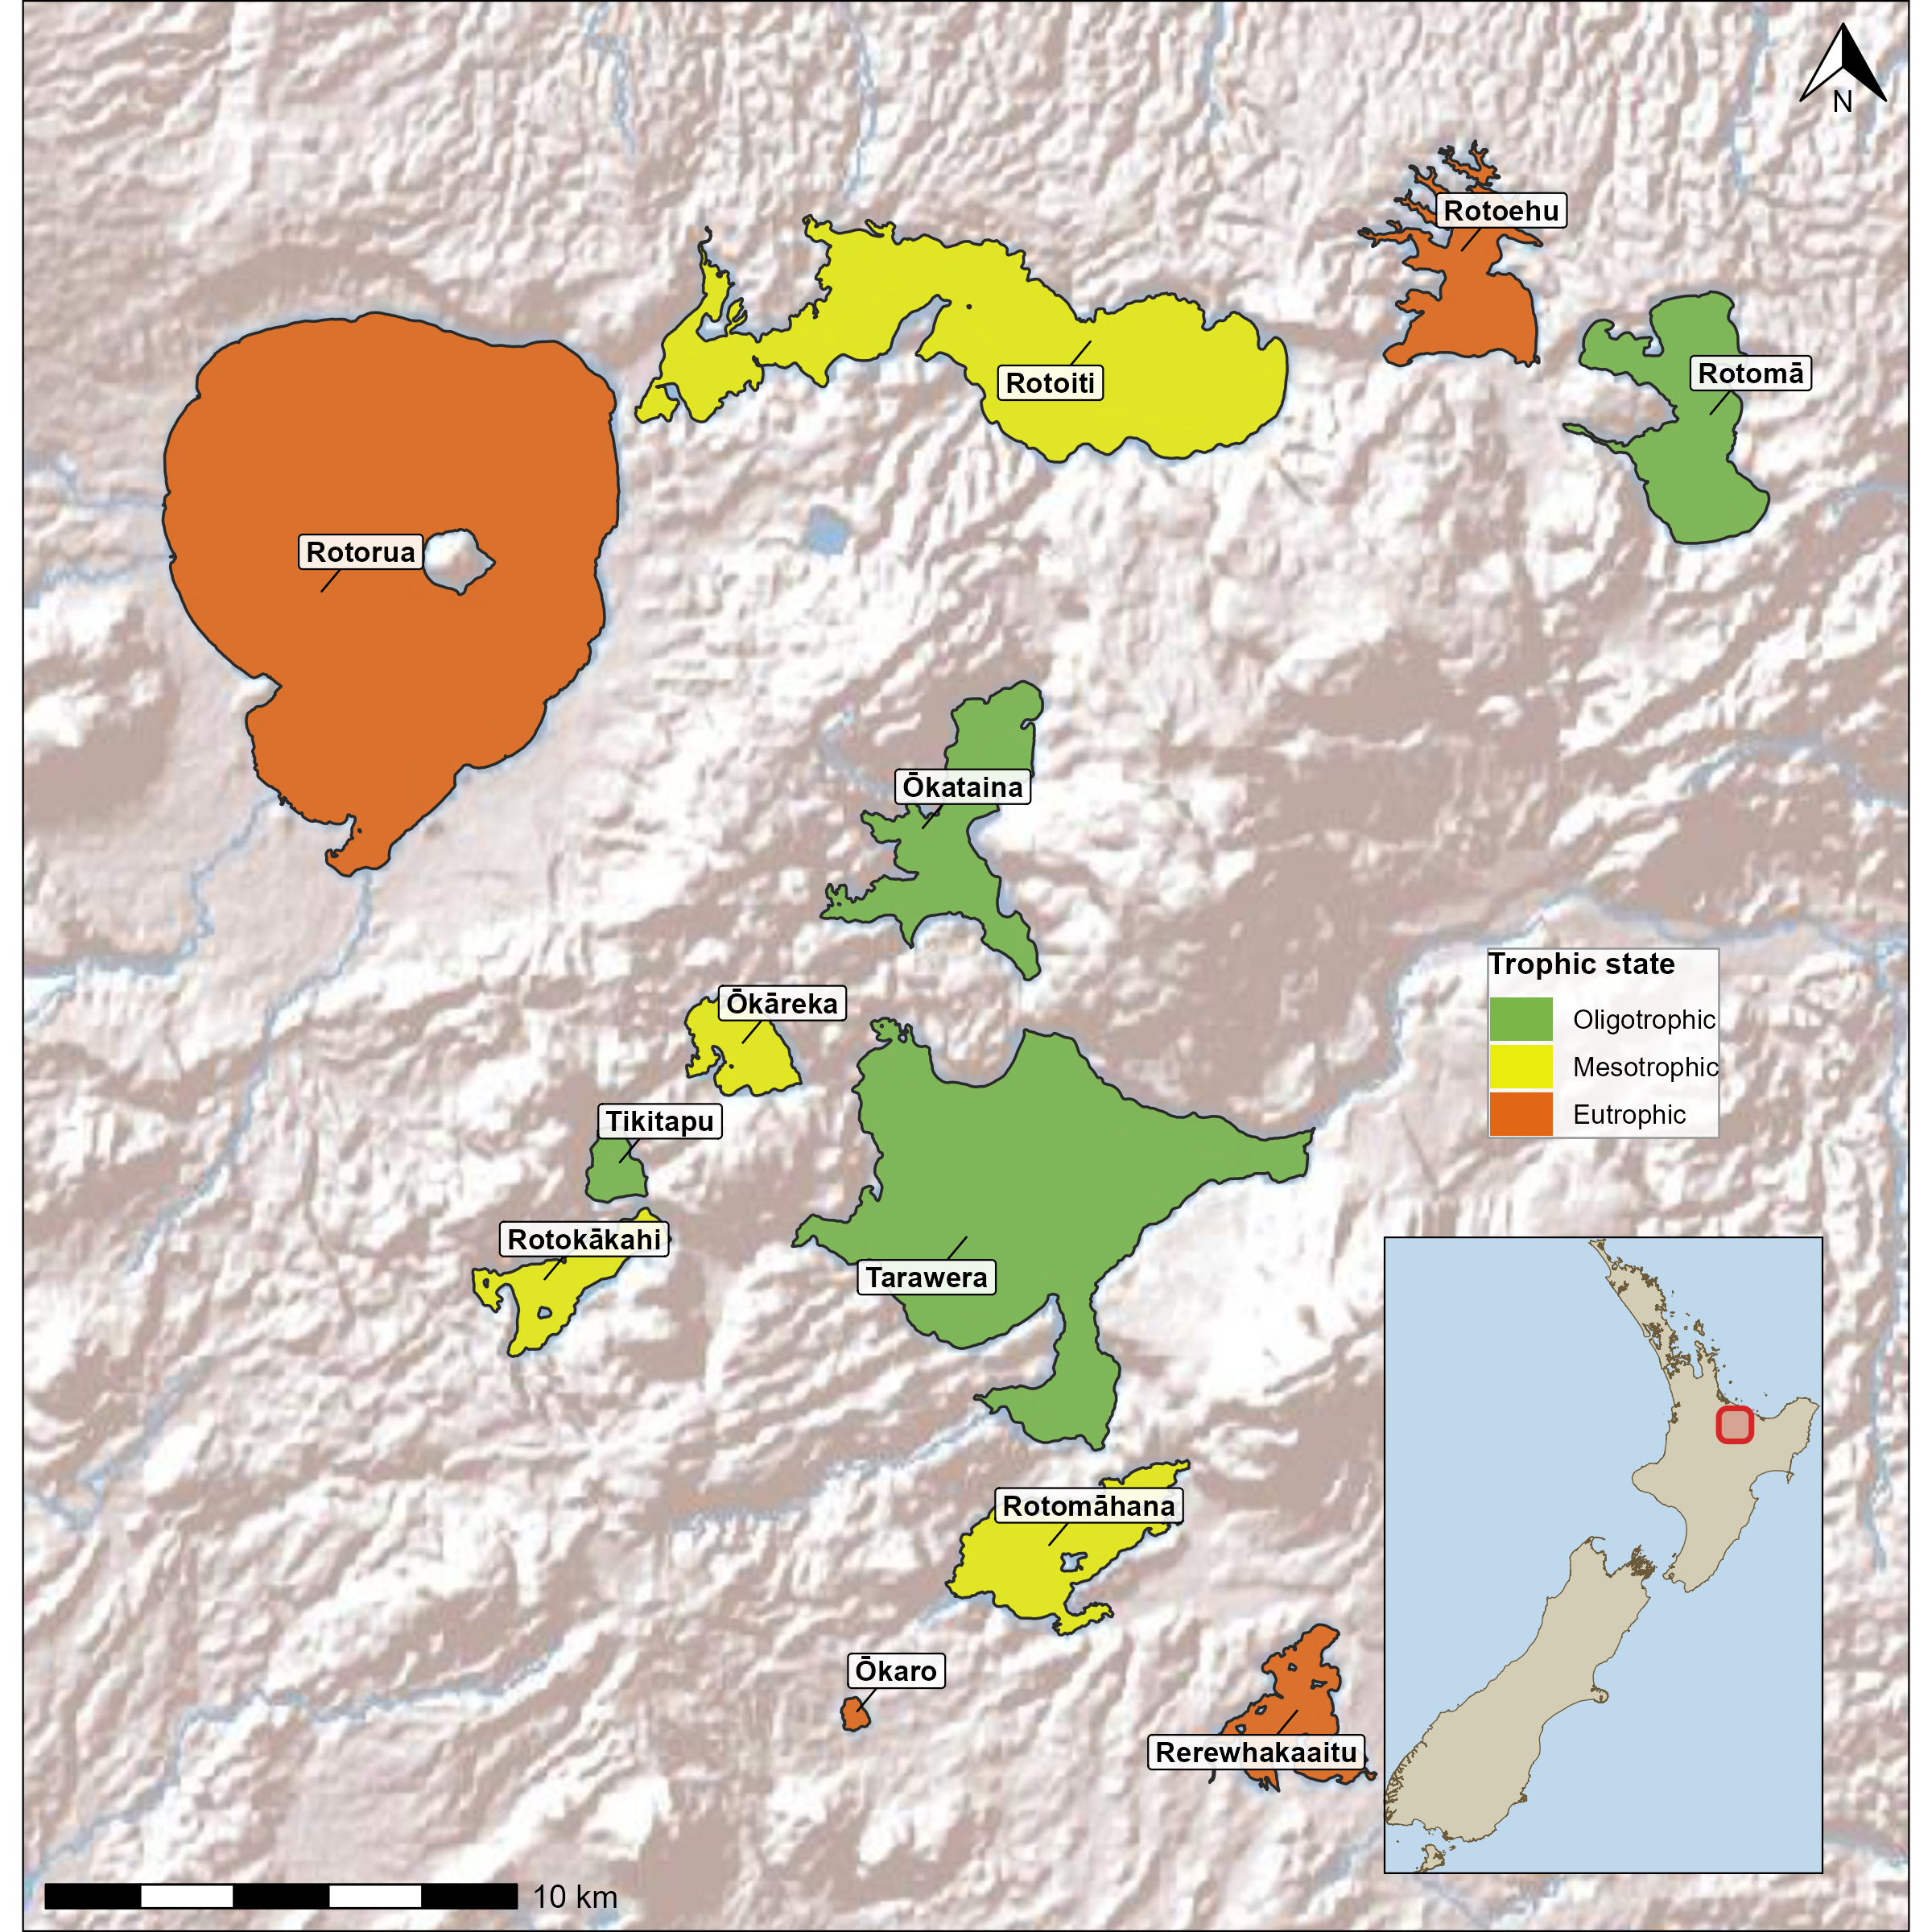
\includegraphics[width=0.65\linewidth,height=\textheight,keepaspectratio]{outputs/fig-study-lakes-map.png}

}

\caption{\label{fig-study-lakes-map}Rotorua Te Arawa Lakes overview map.
Colours represent the trophic state of each lake. Data sourced from:
(LAWA 2025).}

\end{figure}%

\begin{landscape}\begingroup\fontsize{7}{9}\selectfont

\begin{longtable}[t]{lrrrrrrrll}

\caption{\label{tbl-bop-lake-overview}Physical and limnological
characteristics of the twelve Rotorua Te Arawa Lakes. Data sourced from:
LAWA (2025). Lakes Rotorua and Rotoiti have established catfish
populations and Lakes Ōkaro and Rotomāhana have no kōura populations.}

\tabularnewline

\toprule
Lake name & Surface area (km²) & Perimeter length (km) & Catchment area (km²) & Mean depth (m) & Max depth (m) & Depth ratio & Elevation (m) & Mixing regime & Trophic state\\
\midrule
\cellcolor{gray!8}{Rotorua} & \cellcolor{gray!8}{81.0} & \cellcolor{gray!8}{45} & \cellcolor{gray!8}{508.0} & \cellcolor{gray!8}{11.0} & \cellcolor{gray!8}{45.0} & \cellcolor{gray!8}{0.24} & \cellcolor{gray!8}{280} & \cellcolor{gray!8}{Polymictic} & \cellcolor{gray!8}{Eutrophic}\\
Rotoiti & 34.0 & 61 & 123.7 & 31.5 & 124.0 & 0.25 & 279 & Monomictic & Mesotrophic\\
\cellcolor{gray!8}{Rotoehu} & \cellcolor{gray!8}{8.0} & \cellcolor{gray!8}{40} & \cellcolor{gray!8}{49.2} & \cellcolor{gray!8}{8.0} & \cellcolor{gray!8}{13.5} & \cellcolor{gray!8}{0.59} & \cellcolor{gray!8}{295} & \cellcolor{gray!8}{Polymictic} & \cellcolor{gray!8}{Eutrophic}\\
Rotomā & 11.0 & 24 & 27.8 & 36.9 & 83.0 & 0.44 & 316 & Monomictic & Oligotrophic\\
\cellcolor{gray!8}{Ōkataina} & \cellcolor{gray!8}{11.0} & \cellcolor{gray!8}{29} & \cellcolor{gray!8}{59.8} & \cellcolor{gray!8}{39.4} & \cellcolor{gray!8}{78.5} & \cellcolor{gray!8}{0.50} & \cellcolor{gray!8}{305} & \cellcolor{gray!8}{Monomictic} & \cellcolor{gray!8}{Oligotrophic}\\
\addlinespace
Ōkāreka & 3.0 & 11 & 19.6 & 20.0 & 33.5 & 0.60 & 355 & Monomictic & Mesotrophic\\
\cellcolor{gray!8}{Tikitapu} & \cellcolor{gray!8}{1.0} & \cellcolor{gray!8}{5} & \cellcolor{gray!8}{6.2} & \cellcolor{gray!8}{18.0} & \cellcolor{gray!8}{27.5} & \cellcolor{gray!8}{0.65} & \cellcolor{gray!8}{355} & \cellcolor{gray!8}{Monomictic} & \cellcolor{gray!8}{Oligotrophic}\\
Rotokākahi & 4.0 & 16 & 18.7 & 17.5 & 32.0 & 0.55 & 395 & Monomictic & Mesotrophic\\
\cellcolor{gray!8}{Tarawera} & \cellcolor{gray!8}{41.0} & \cellcolor{gray!8}{48} & \cellcolor{gray!8}{143.1} & \cellcolor{gray!8}{50.0} & \cellcolor{gray!8}{87.5} & \cellcolor{gray!8}{0.57} & \cellcolor{gray!8}{305} & \cellcolor{gray!8}{Monomictic} & \cellcolor{gray!8}{Oligotrophic}\\
Rotomāhana & 9.0 & 27 & 83.3 & 60.0 & 125.0 & 0.48 & 340 & Monomictic & Mesotrophic\\
\addlinespace
\cellcolor{gray!8}{Ōkaro} & \cellcolor{gray!8}{0.3} & \cellcolor{gray!8}{2} & \cellcolor{gray!8}{3.9} & \cellcolor{gray!8}{12.5} & \cellcolor{gray!8}{18.0} & \cellcolor{gray!8}{0.69} & \cellcolor{gray!8}{280} & \cellcolor{gray!8}{Monomictic} & \cellcolor{gray!8}{Eutrophic}\\
Rerewhakaaitu & 5.0 & 25 & 37.0 & 7.0 & 15.8 & 0.44 & NA & Polymictic & Eutrophic\\
\bottomrule

\end{longtable}

\endgroup{}
\end{landscape}

The lake beds are owned by the Te Arawa Lakes Trust (TALT), with the
exception of Lake Rotokākahi, which remains under the guardianship of
Tuhourangi and Ngāti Tumatawera iwi. TALT, in collaboration with Te
Komiti Whakahaere, oversees the harvest of ngā taonga in the Te Arawa
Lakes under a mahere whakahaere (Fisheries Management Plan; Te Arawa
Lakes Trust (2015)), reflecting the deep cultural and ecological
significance of the lakes to Te Arawa iwi and hapū.

Each lake supports a mix of native and introduced species. Alongside
kōura and catfish discussed above, native taxa include the freshwater
mussel kākahi (\emph{Echyridella menziesii}), kōaro (\emph{Galaxias
brevipinnis}), bullies (toitoi; \emph{Gobiomorphus cotidianus}), longfin
eel (tuna; \emph{Anguilla dieffenbachii}), and common smelt
(\emph{Retropinna retropinna}). Introduced species include brown and
rainbow trout (\emph{Salmo trutta}, \emph{Oncorhynchus mykiss}),
mosquitofish (\emph{Gambusia affinis}), and goldfish (morihana;
\emph{Carassius auratus}). The lakes also support a mix of native
macrophytes and several invasive species that have transformed the
littoral zone in many lakes (Figure~\ref{fig-rotoiti-weeds}) (Burton
2017). Current lake management prioritises improving water quality and
controlling invasive species. This includes alum dosing (aluminium
sulphate) in Lakes Rotorua and Ōkaro to reduce phosphorus loading,
mechanical and chemical control of invasive macrophytes, and the
community-led ``Catfish Killas'' programme, which aims to reduce catfish
abundance from the lakes.

\begin{figure}

\centering{

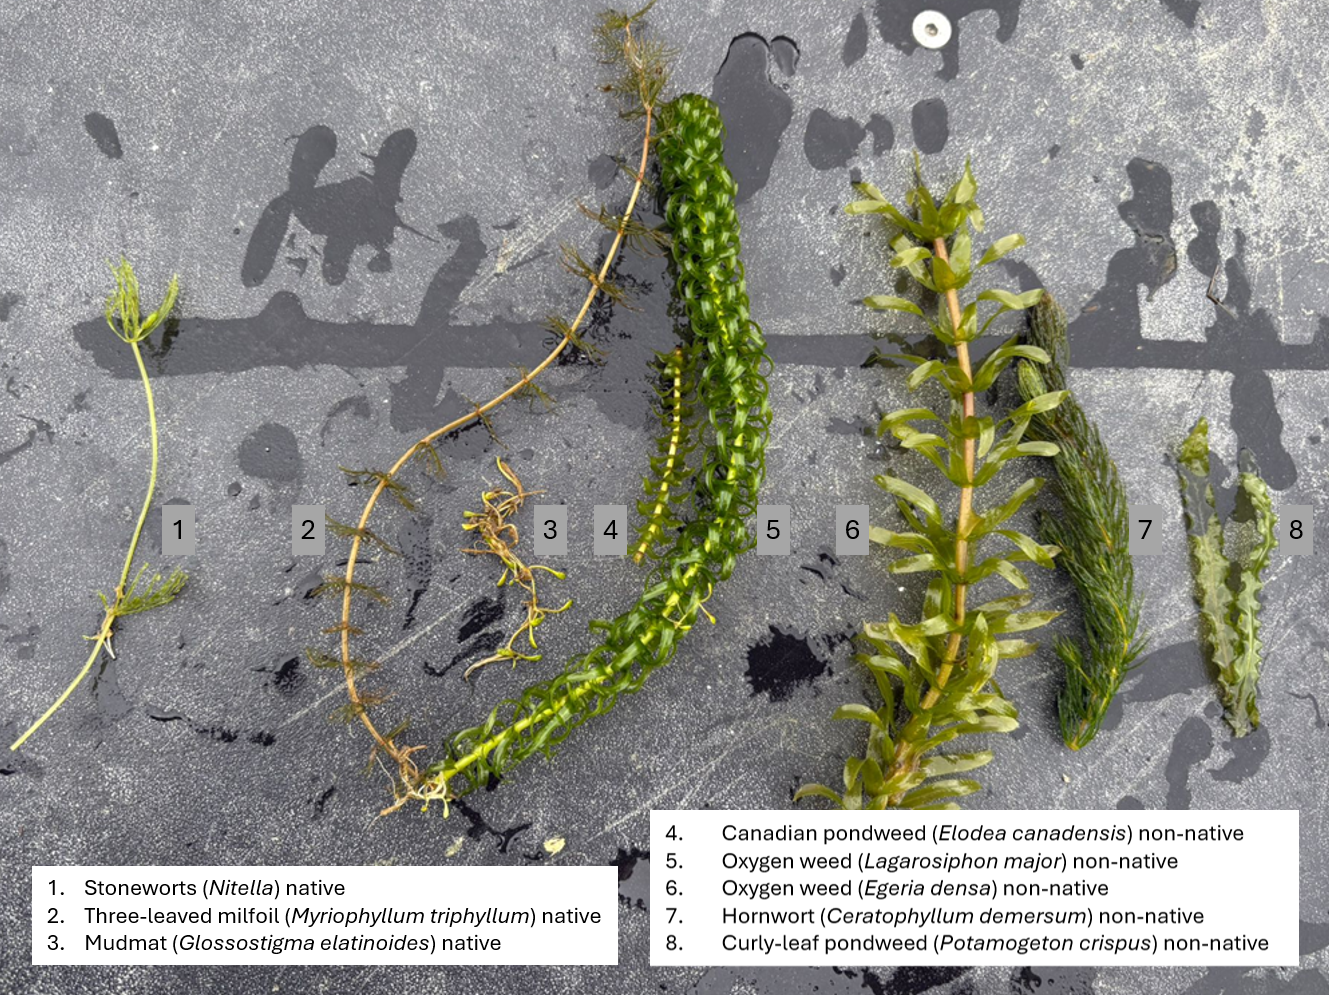
\includegraphics[width=0.8\linewidth,height=\textheight,keepaspectratio]{images/fig-rotoiti-weeds.png}

}

\caption{\label{fig-rotoiti-weeds}Photo of some of the native and
non-native macrophyte species found in Lake Rotoiti.}

\end{figure}%

\section{Compounding threats to kōura
habitat}\label{compounding-threats-to-kux14dura-habitat}

In addition to predation by catfish, kōura face multiple interacting
stressors that progressively restrict the habitat available to them
(Kusabs et al. 2015a; Lee et al. 2025). Kōura use rocky habitats or
deeper parts of the lake which provides refuge from predators during the
day (Jowett et al. 2008; Kusabs et al. 2015b) and at night, kōura
migrate vertically into the productive littoral zone to forage (Devcich
1979). The use of both shallow and deep habitats means that, for kōura
to thrive, both must remain accessible and habitable.

In stratified lakes during summer and autumn, thermal stratification can
create anoxic conditions below the thermocline. Since kōura avoid
dissolved oxygen concentrations below 5 mg/L (Devcich 1979), this
displace kōura from their daytime deep refuge into the shallow littoral
zone (Kusabs et al. 2026), placing kōura in the depth range where
catfish predation pressure is greatest (Blanchfield et al. 2026). The
result is a seasonal compression of available habitat, where suitable
depths shrink to precisely the zone where predation risk is highest
(Kusabs et al. 2026). This means that for

The importance of an oxygenated deep refuge is illustrated by Lake Taupō
(maximum depth 186 m), where catfish and kōura demonstrate a more stable
co-existence because deep waters remain oxygenated below the thermocline
year-round (Verburg and Albert 2019), providing continuous suitable
habitat for kōura (Kusabs and Taiaroa 2015). In Lake Rotoiti, this deep
refuge becomes anoxic and unavailable for kōura (Kusabs et al. 2026).

The shallow refuge available to kōura is also being progressively
reduced as lake surface water temperatures increase above the kōura
optimal temperature threshold of 21 °C (Devcich 1979). Furthermore,
dense beds of invasive macrophytes obstruct kōura movement through the
littoral zone and reduce access to foraging habitat (Kusabs and Quinn
2009). When these macrophyte beds collapse, the subsequent decomposition
further intensifies oxygen depletion in deeper waters (Vincent et al.
1984; Hamilton et al. 2005). The cumulative effect of these stressors
can be visualised by estimating the proportion of each lake's bottom
area that remains ``liveable'' --- meaning sufficiently oxygenated and
within thermal optimum for kōura. Across eleven of the Rotorua Te Arawa
Lakes, liveable habitat varies strongly with season, with sharp summer
declines in eutrophic and shallow lakes such as Rotorua, Rotoiti, Ōkaro,
and Rotomāhana, while deeper oligotrophic lakes such as Rotomā,
Tarawera, and Tikitapu remain relatively stable year-round
(Figure~\ref{fig-livable-habitat-summary}). Over the past
\textasciitilde20 years several lakes show statistically significant
declines in annual mean liveable habitat, with Ōkāreka declining -0.4 \%
per year (Figure~\ref{fig-livable-habitat-trends}).

Climate change is expected to intensify all of these pressures. Stronger
and longer thermal stratification will expand and prolong anoxic
conditions below the thermocline (Woolway et al. 2021), while warming
surface waters are projected to expand the range of suitable catfish
habitat in Aotearoa (Lee et al. 2025). The compression of suitable kōura
habitat documented here is therefore likely to accelerate, reinforcing
the need to understand which habitats kōura prefer and whether habitat
enhancement can build resilience in kōura populations. This rationale is
supported by evidence from other systems supporting crayfish: in lakes
where muddy substrates provide limited refugia, adding rocky substrate
has been shown to relax refugia limitation and increase noble crayfish
(\emph{Astacus astacus}) population density (Johnsen and Taugbøl 2008).
Structural addition can only deliver this benefit when water quality
falls within species tolerance, as when dissolved oxygen or temperature
exceeds physiological limits, species cannot persist regardless of
refuge quality.

\begin{figure}

\centering{

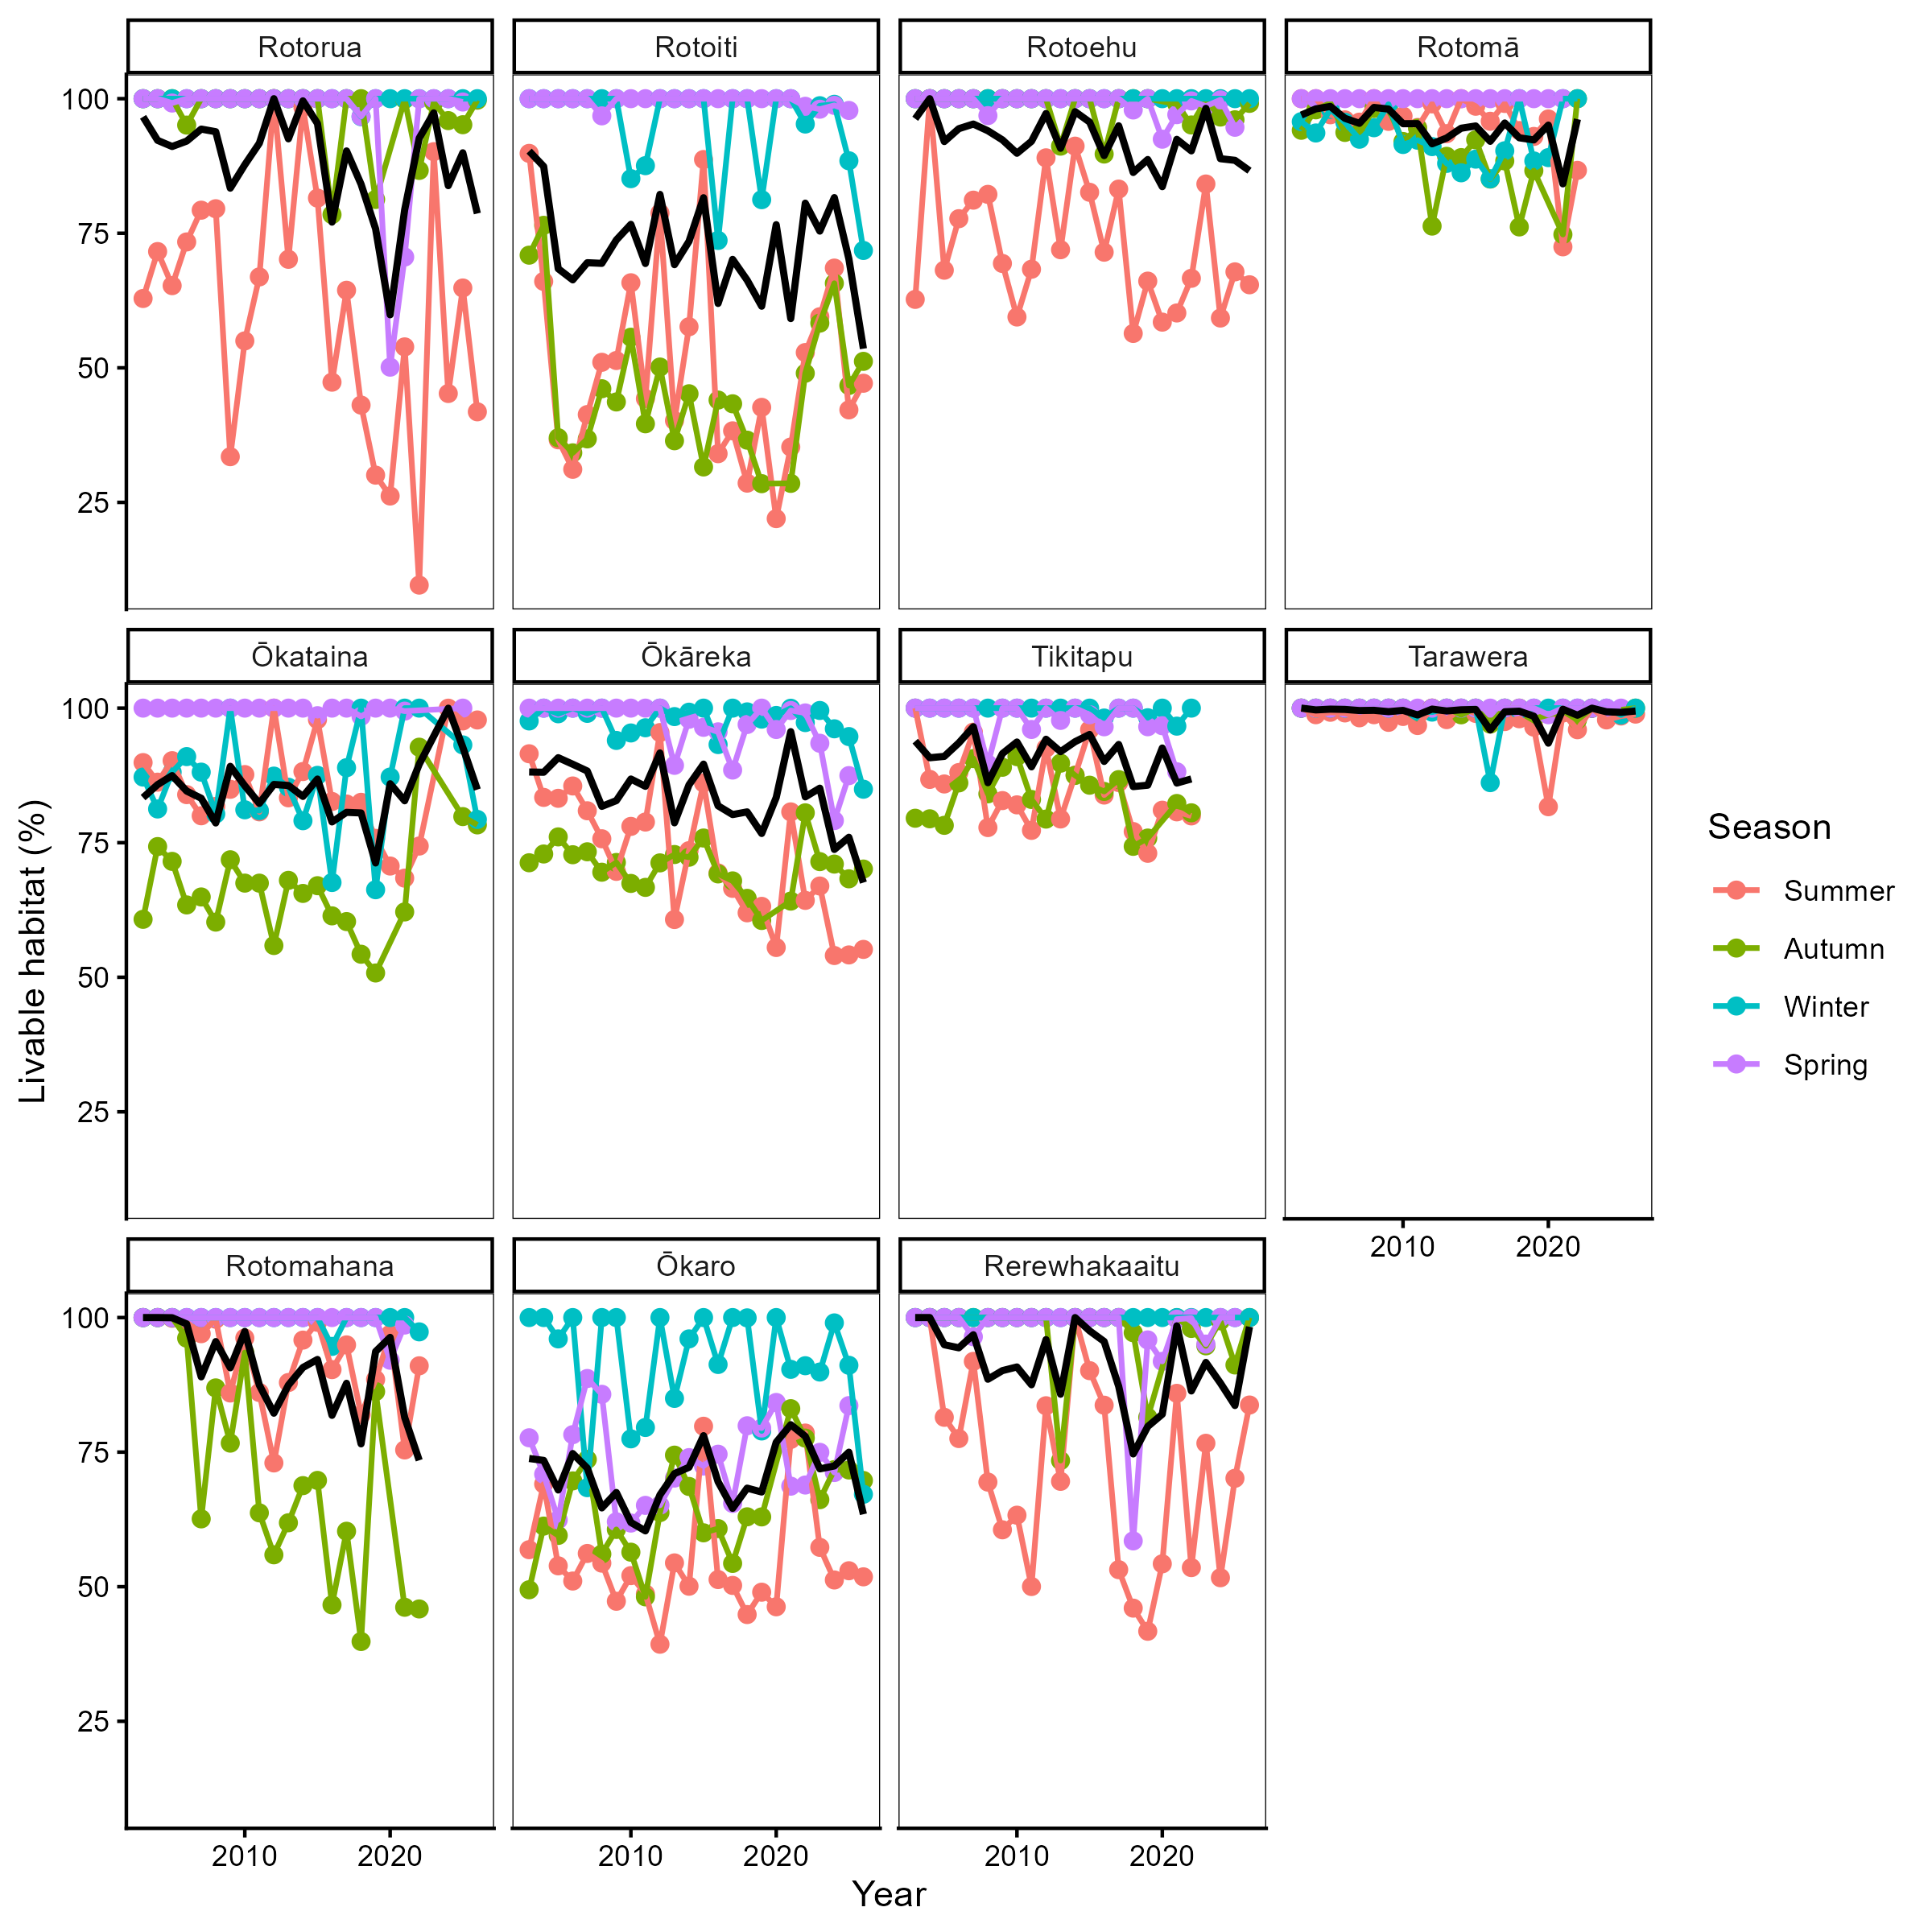
\includegraphics[width=1\linewidth,height=\textheight,keepaspectratio]{outputs/fig-livable-habitat-summary.png}

}

\caption{\label{fig-livable-habitat-summary}Liveable habitat (\%) for
kōura across eleven of the Rotorua Te Arawa Lakes from 2003 to 2026, by
season. Liveable habitat is defined as the proportion of the water
column meeting dissolved oxygen (\textgreater{} 5 mg/L) and temperature
(\textless{} 21 °C) thresholds suitable for kōura. Coloured lines show
seasonal means; the black line shows the overall trend. Derived from CTD
cast data collected by BOPRC monthly monitoring and monitoring buoy data
LimnoTrack (Moore and McBride 2026).}

\end{figure}%

\begin{figure}

\centering{

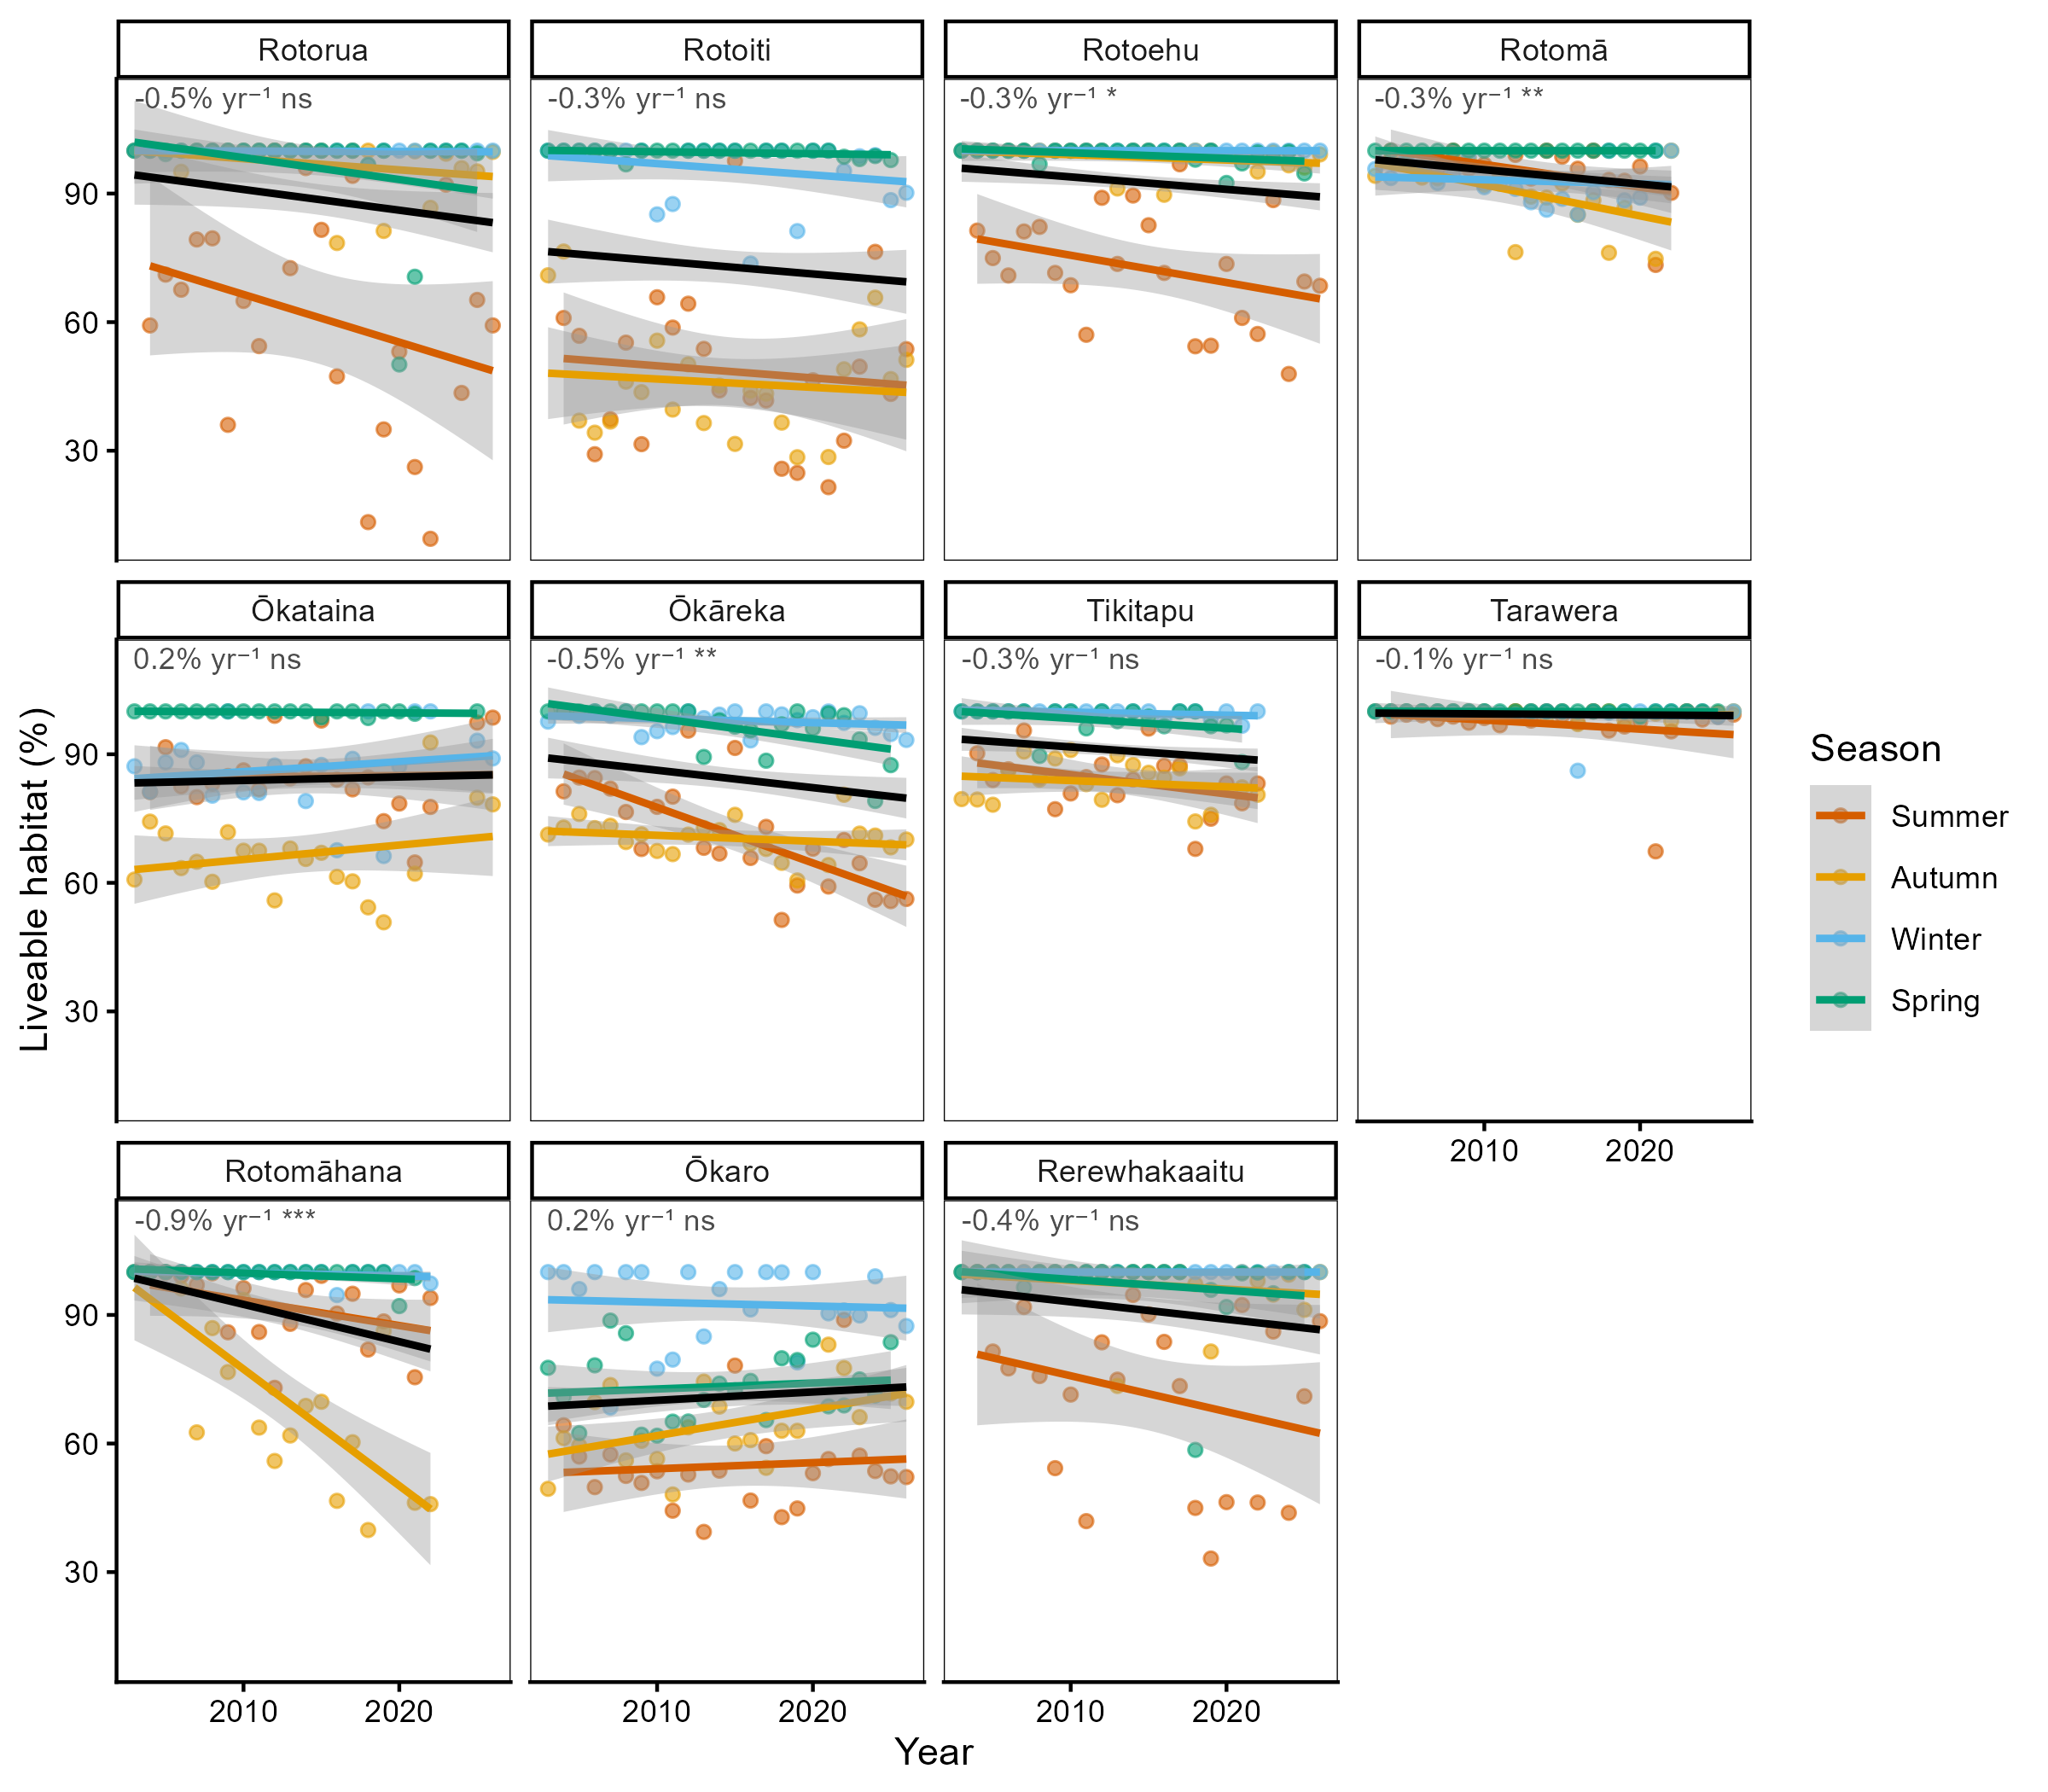
\includegraphics[width=1\linewidth,height=\textheight,keepaspectratio]{outputs/fig-livable-habitat-trends.png}

}

\caption{\label{fig-livable-habitat-trends}Long-term trends in seasonal
and annual mean liveable habitat for kōura across eleven of the Rotorua
Te Arawa Lakes. Liveable habitat is defined as the proportion of the
lake bottom area meeting dissolved oxygen (\textgreater{} 5 mg/L) and
temperature (\textless{} 21 °C) thresholds suitable for kōura. Points
represent means; lines show linear regressions with 95 \% confidence
intervals. Annual slopes are reported as percentage change per year
(significance: *** p \textless{} 0.001, ns = not significant). Derived
from CTD cast data collected by BOPRC monthly monitoring and monitoring
buoy data LimnoTrack (Moore and McBride 2026).}

\end{figure}%

\section{Knowledge gaps and thesis
aims}\label{knowledge-gaps-and-thesis-aims}

The previous sections established that kōura populations in the Rotorua
Te Arawa Lakes are declining because of multiple interacting pressures,
such as invasive predation, eutrophication, thermal stratification, and
macrophyte expansion. It was also shown that their suitable habitat is
both seasonally compressed and progressively shrinking (Kusabs et al.
2026). Although the broad drivers of decline are increasingly well
understood, several critical knowledge gaps limit our ability to design
effective interventions, particularly around how kōura interact
behaviourally with catfish as a novel predator, and around the role of
habitat structure and refugia in mediating those predator-prey
interactions, questions relevant to freshwater prey species facing novel
predators globally.

First, while catfish are implicated as a key driver of kōura decline,
the effect catfish have on kōura behaviour leading to non-consumptive
effects in comparison with native predators had not been quantified. I
therefore conducted aquarium experiments in which kōura refuge use was
recorded when exposed to native longfin eels and to catfish. I expected
that kōura would show no response to catfish consistent with predator
naïveté (Sih et al. 2010), or that they would show stronger antipredator
responses to the novel catfish than to native eels, consistent with
generalised fear response (Sih et al. 2023).

Second, the natural habitats that kōura prefer had been described in
streams and deeper parts of lakes but which shoreline habitat features
kōura prefer remained unknown. I therefore monitored kōura presence at
60 shoreline sites across five of the Rotorua Te Arawa Lakes, recording
habitat features and fish species. I expected that rocky substrates with
high structural complexity would be the primary predictor of kōura
presence, consistent with stream habitat studies (Olsson 2008; Jowett et
al. 2008).

Third, although the deployment of habitat enhancement structures had
been applied in freshwater systems globally to support fish and
invertebrates (Smokorowski and Pratt 2007; Santos et al. 2011), few
studies had tested which combinations of material and structural
configuration best support crayfish specifically. I therefore designed
and tested multiple shelters configurations using wood and stone in
mesocosm experiments. I expected that configurations providing multiple
crevices of varying sizes would be preferred by the widest range of
kōura, including juveniles.

Finally, no field deployments of habitat enhancement structures for
kōura in lakes had previously been reported. Therefore, I deployed stone
piles in Lake Rotoiti and expected that kōura populations at the stone
piles would increase, as providing more refuge habitat would allow more
kōura to avoid predators. A secondary aim of the final study was to
identify potential unintended consequences of habitat enhancement,
including the risk that structures may provide refuge for catfish.

This thesis addresses each of these gaps in turn through four research
chapters, building from behavioural mechanisms in controlled conditions,
through natural habitat use, to structure design, and finally to field
deployment.

\section{Research questions and thesis
structure}\label{research-questions-and-thesis-structure}

This thesis pursued two complementary sets of aims. The first was to
advance fundamental ecological knowledge about how a naïve prey species
responds behaviourally to a novel predator, and about the role of
habitat structure in mediating predator-prey interactions, questions
with global relevance to freshwater systems facing invasive species. The
second was applied: to identify optimal strategies for restoring and
enhancing kōura populations in the Rotorua Te Arawa Lakes through
structural habitat enhancement. The findings of this thesis are reported
in the following four research chapters, followed by a synthesis and a
general conclusion (Table~\ref{tbl-research-questions}).

\begin{longtable}[]{@{}
  >{\centering\arraybackslash}p{(\linewidth - 4\tabcolsep) * \real{0.1212}}
  >{\raggedright\arraybackslash}p{(\linewidth - 4\tabcolsep) * \real{0.2727}}
  >{\raggedright\arraybackslash}p{(\linewidth - 4\tabcolsep) * \real{0.6061}}@{}}
\caption{Research questions addressed in each thesis
chapter.}\label{tbl-research-questions}\tabularnewline
\toprule\noalign{}
\begin{minipage}[b]{\linewidth}\centering
RQ
\end{minipage} & \begin{minipage}[b]{\linewidth}\raggedright
Chapter
\end{minipage} & \begin{minipage}[b]{\linewidth}\raggedright
Research question
\end{minipage} \\
\midrule\noalign{}
\endfirsthead
\toprule\noalign{}
\begin{minipage}[b]{\linewidth}\centering
RQ
\end{minipage} & \begin{minipage}[b]{\linewidth}\raggedright
Chapter
\end{minipage} & \begin{minipage}[b]{\linewidth}\raggedright
Research question
\end{minipage} \\
\midrule\noalign{}
\endhead
\bottomrule\noalign{}
\endlastfoot
1 & 2 --- Native vs.~Novel Threats & How do native and non-native
predators differentially influence antipredator behaviour and refuge use
in kōura? \\
2 & 3 --- Where do Kōura Live? & Which natural shoreline features do
kōura prefer? \\
3 & 4 --- The Importance of Structure & Does shelter structure or
material composition drive kōura refuge selection? \\
4 & 5 --- Rock Piles as Kōura Habitat & Can habitat enhancement
structures provide effective habitat for kōura in Lake Rotoiti? \\
\end{longtable}

Before the deployment of any structures, it was first necessary to
understand the response of kōura when exposed to native and novel
predators. Therefore, in \textbf{Chapter 2}, kōura were exposed to
native eels and to novel catfish in an aquarium study where refuge use
was analysed. In \textbf{Chapter 3}, the natural preferred shoreline
habitat for kōura was investigated by monitoring 60 sites over five
lakes. From this we gained a clearer picture of which habitat features
support kōura and which shoreline areas would most benefit from
structural enhancement. In the next chapter, \textbf{Chapter 4}, we
designed and tested shelter types to determine kōura preference. Kōura
are known to use various materials and compositions, so for this study
we tested different configurations of wood and stone structures in
mesocosm experiments to determine kōura shelter preferences. With an
optimal design identified, \textbf{Chapter 5} deployed five stone pile
structures along the shoreline in Lake Rotoiti and monitored kōura
colonisation and abundance development over 18 months. \textbf{Chapter
6} synthesises the findings across all four research chapters,
incorporating two pilot case studies: a stone pile deployment in Lake
Ōkaro where water quality and kōura reintroduction were monitored, and a
deeper-water deployment across a depth gradient in Lake Rotoiti assessed
using Remotely Operated Vehicle (ROV) surveys. The chapter concludes
with an overview of the findings and considers how structural habitat
enhancement can contribute to building resilience in declining
freshwater crayfish populations more broadly. As each of the four
research chapters are written as stand-alone manuscripts, some overlap
of background information and methods is unavoidable. However, the
general introduction provides a comprehensive overview of the study
system, the species involved, and the research questions addressed in
this thesis.

\clearpage
\providecommand{\chaptermark}[1]{}
\ifcsname c@chapter\endcsname
\setcounter{chapter}{2}
\setcounter{figure}{0}
\setcounter{table}{0}
\setcounter{section}{0}
\addcontentsline{toc}{chapter}{\protect\numberline{2}Native vs.\ Novel Threats}
\chaptermark{Native vs.\ Novel Threats}
\fi
\providecommand{\thechapter}{2}
\thispagestyle{empty}
\begin{tikzpicture}[remember picture, overlay]
  \begin{scope}
    \clip ([yshift=-7cm]current page.north west)
          rectangle ([yshift=4.5cm]current page.south east);
    \node[inner sep=0pt, anchor=north]
      at ([yshift=-7cm]current page.north)
      {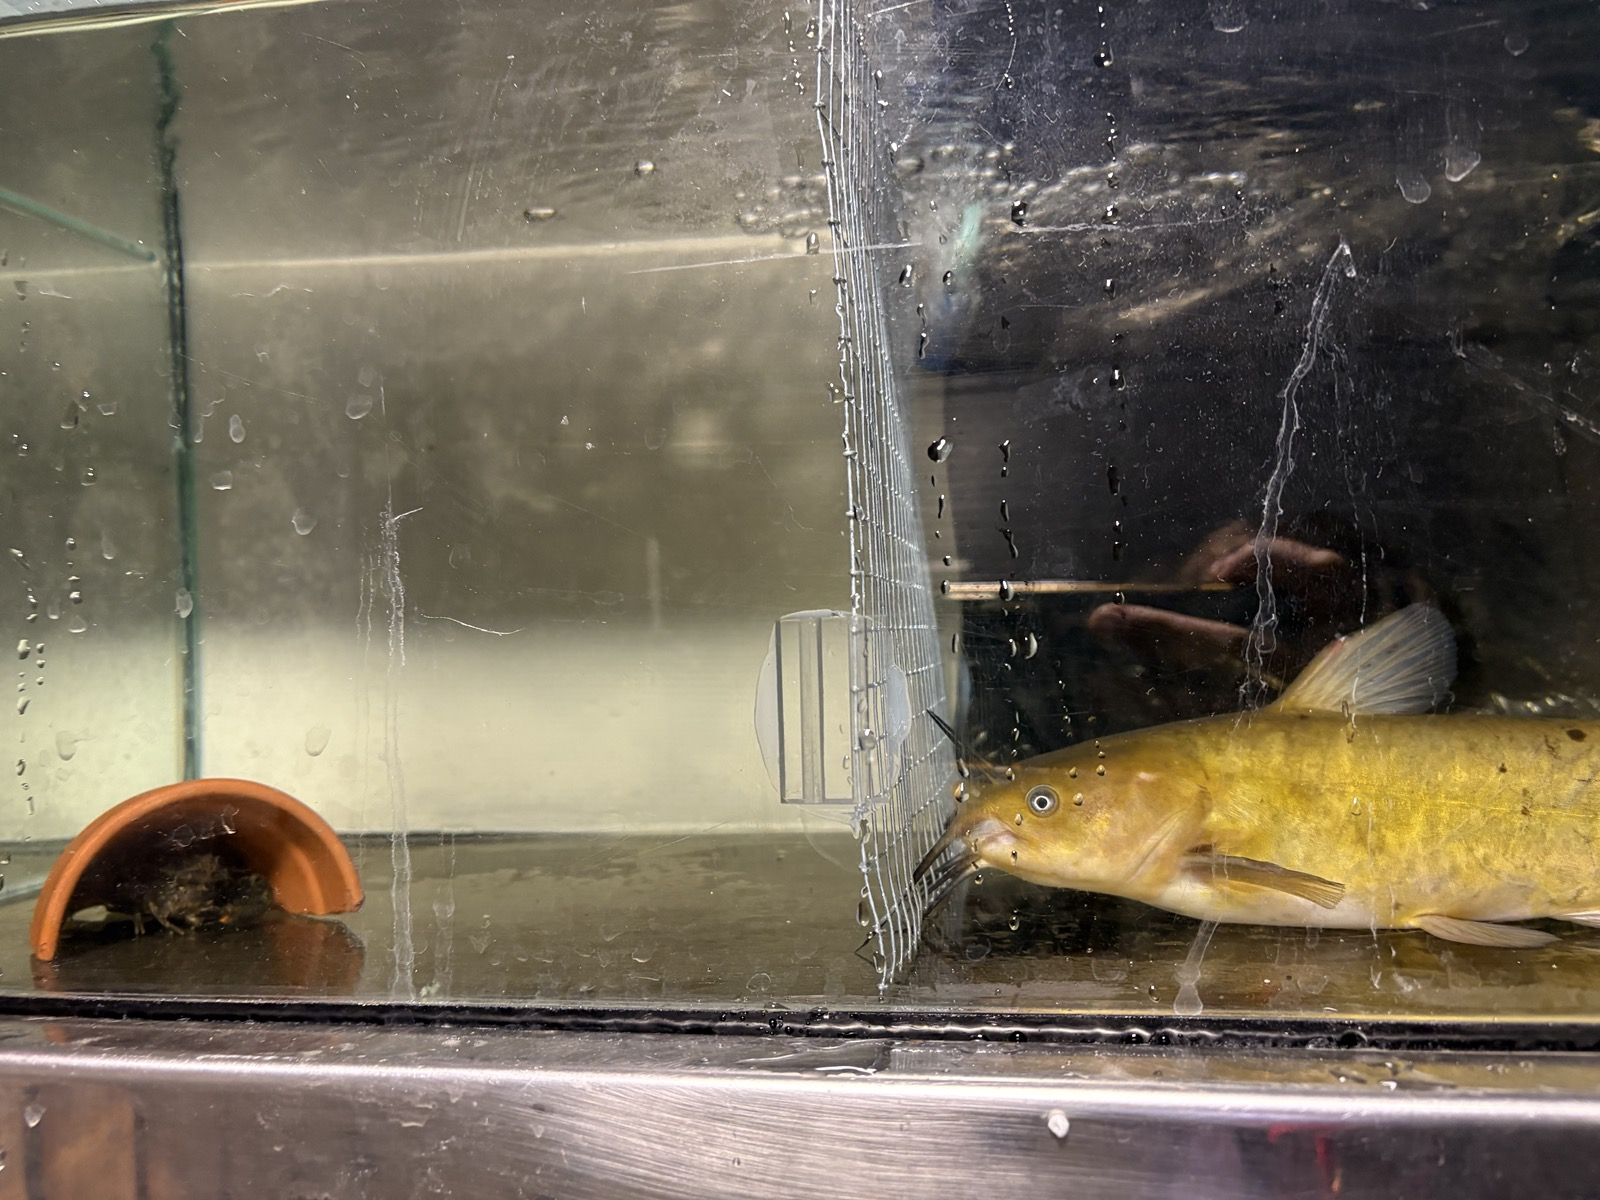
\includegraphics[height=18.2cm]{images/ch2_cover.jpg}};
  \end{scope}
  \fill[black]
    (current page.north west) rectangle ([yshift=-7cm]current page.north east);
  \node[color=thesissand, align=left,
        font=\fontsize{13}{16}\selectfont\sffamily, anchor=west]
    at ([xshift=1.5cm, yshift=-1.5cm]current page.north west)
    {Chapter \thechapter};
  \node[color=white, text width=0.85\paperwidth, align=left,
        font=\fontsize{22}{28}\selectfont\bfseries\sffamily, anchor=west]
    at ([xshift=1.5cm, yshift=-4cm]current page.north west)
    {Native vs.\ Novel Threats};
  \node[color=white, text width=0.85\paperwidth, align=left,
        font=\fontsize{10}{13}\selectfont\itshape\sffamily, anchor=north west]
    at ([xshift=1.5cm, yshift=-5.0cm]current page.north west)
    {Fear of the new: a predatory invader provokes stronger non-consumptive effects on a keystone native prey than a native predator};
  \fill[black]
    (current page.south west) rectangle ([yshift=4.5cm]current page.south east);
  \node[color=white, text width=0.85\paperwidth, align=left,
        font=\fontsize{9}{13}\selectfont\sffamily, anchor=west]
    at ([xshift=1.5cm, yshift=3.2cm]current page.south west)
    {Olivier V.\ Raven, Calum MacNeil, Finnbar Lee, Robin Holmes, Ian A. K.\ Kusabs, Francis J.\ Burdon \& Deniz Özkundakci};
  \node[color=thesissand, text width=0.85\paperwidth, align=left,
        font=\fontsize{9}{13}\selectfont\itshape\sffamily, anchor=west]
    at ([xshift=1.5cm, yshift=1.5cm]current page.south west)
    {Biological Invasions --- Under review};
\end{tikzpicture}
\null
\clearpage

\section*{Abstract}\label{abstract-1}
\addcontentsline{toc}{section}{Abstract}

The non-consumptive effects (NCEs) of predators on prey result in costly
antipredator behaviours, including increased refuge use and reduced
foraging. NCEs significantly influence prey population dynamics,
community interactions, and affect ecosystem functioning, particularly
when the prey are keystone species. In Aotearoa-New Zealand, the native
freshwater crayfish kōura (\emph{Paranephrops planifrons}) is a keystone
species with an important functional role affecting sediment
bioturbation, nutrient cycling, and benthic community structure. Kōura
are preyed upon by multiple predators including native longfin eel
(\emph{Anguilla dieffenbachii}) and invasive brown bullhead catfish
(\emph{Ameiurus nebulosus}). Under laboratory conditions, we tested
whether visual and chemical cues from these two predators induced
different refuge-seeking and feeding behaviour responses by kōura.
Predator presence produced in the dark a NCE on refuge use, with kōura
exposed to catfish showing significantly greater refuge-seeking
behaviour than those exposed to eels. This result is consistent with the
generalisation theory triggered by unfamiliar predator cues rather than
classic prey naivety. Our study indicates catfish incursions may provoke
a greater NCE on kōura behaviours than resident eels. As catfish range
expansion continues, these NCEs may represent an ecologically
significant and underappreciated threat to kōura populations,
compounding the direct predation pressure already documented for this
invader.

\section{Introduction}\label{introduction}

Biological invasions can have profound impacts on invaded ecosystems,
particularly through the introduction of novel predators that prey upon
naïve native species lacking coevolved defence mechanisms (Doherty et
al. 2016). Native prey may be naïve not just to a specific invader, but
to entire functional groups of predators, making them especially
vulnerable to direct predation when an invasion introduces a predator
type entirely absent from their evolutionary history (Sih et al. 2010;
Carthey and Banks 2014). In addition to these consumptive effects,
native prey may exhibit heightened fear responses to invasive predators,
leading to the development of anti-predator behaviours such as increased
refuge use and avoidance of open habitats (Kindinger and Albins 2017).
These behavioural changes, termed non-consumptive effects (NCEs), can
substantially influence population dynamics by reducing foraging
activity, growth, and reproductive output (Preisser et al. 2005). In
contrast, native predators generally elicit different responses because
prey and predators have coevolved, resulting in behavioural and
physiological adaptations that stabilise predator--prey interactions
(Abrams 2000).

Chemical signals (kairomones) are a key component of NCEs (Kasumyan
2022). Freshwater crayfish release and detect kairomones to help
navigate aquatic environments and mediate interactions with predatory
fish (Blake and Hart 1993; Brönmark and Hansson 2012; Wood and Moore
2020a). Kairomones carry signals via excreta, mucus, or skin, that
crayfish use to detect predators (Appelberg et al. 1993). Crayfish
respond more strongly to signals from predators that have consumed
conspecifics and to alarm cues released when conspecifics are injured or
killed (Gherardi et al. 2011; Beattie and Moore 2018). The NCEs due to
kairomone detection include reduced growth, reduced activity levels
(Adams 2007; Ramberg-Pihl and Yurewicz 2020), and altered social
dynamics like the use of refuge spaces (Driscoll et al. 2020).
Non-predatory fish can also trigger behaviour changes, likely through an
increased awareness of potential risk (Nyström 2005). However, the
strength of these responses depends on prior experience as wild-caught
individual crayfish show stronger antipredator responses than farmed
conspecifics naïve to predators (Martin 2014), indicating that both
learnt behaviour and evolutionary history shape kairomone detection.

In Aotearoa-New Zealand (hereafter Aotearoa), the endemic northern
freshwater crayfish \emph{Paranephrops planifrons} (White, 1842) is a
keystone species impacted by non-native species. This crayfish species
is commonly known as kōura and is a taonga (culturally treasured)
species for Māori, the indigenous people of Aotearoa, with strong
cultural values as a food resource (Kusabs and Quinn 2009).
Ecologically, kōura play a critical role as ecosystem engineers through
their effects on sediment dynamics, nutrient cycling, and benthic
community structure (Collier et al. 1997; Parkyn et al. 2001; Usio and
Townsend 2004). Currently, kōura are threatened by multiple stressors,
including climate change, water-quality degradation and invasive
species, contributing to widespread population declines (Lee et al.
2025; Kusabs et al. 2026).

Kōura have a long coevolutionary history with the native longfin eel
(\emph{Anguilla dieffenbachii}) (hereafter eel) and shortfin eel
(\emph{A. australis}) in Aotearoa (Brown 2009; MacNeil et al. 2025).
Reflecting this coevolutionary history, kōura can respond more strongly
to eel kairomones than to those of introduced non-native brown trout
(\emph{Salmo trutta}), even when sourced from streams where both
predators were present (Shave et al. 1994). Shave et al. (1994) suggest
that kōura predator recognition is a fixed behavioural trait shaped by
coevolution. An invasive fish species that threatens kōura is the brown
bullhead catfish (\emph{Ameiurus nebulosus}) (hereafter catfish).
Catfish were introduced to Aotearoa in 1877, and the invasive species
has since spread to multiple lakes and rivers in the North Island
(McDowall 1990; Barnes and Hicks 2003; Dedual 2019). For example, in
2016/18, the presence of catfish was confirmed in two large volcanic
lakes, Lakes Rotoiti and Rotorua in the Bay of Plenty region, which have
historically contained large populations of kōura (Francis 2019; Lee et
al. 2025). Catfish are highly tolerant of a wide range of environmental
conditions (Scott and Crossman 1973; Lee et al. 2025) and their broad
gape and opportunistic feeding behaviour enable the consumption of a
wide variety of aquatic prey (Scott and Crossman 1973; Dedual 2019).
Given Aotearoa lacks native Siluriformes, the recent and ongoing spread
of catfish into North Island waterways represents a truly novel
predation threat to which kōura may lack adequate behavioural or sensory
adaptations to respond.

In this study, we used controlled laboratory experiments to test whether
the presence of a novel and native predator induced differences in kōura
NCEs, specifically refuge-seeking and feeding behaviours. Our
experiments tested the following two hypotheses regarding kōura
behavioural responses to predator cues: 1) Kōura would show less
shelter-seeking behaviour when presented with catfish compared to eels,
due to naivety towards a novel predator (Carthey and Banks 2014); or 2)
kōura would respond more strongly to unfamiliar catfish cues than to the
native eel, consistent with a generalised fear response to a novel
predator type (Sih et al. 2023). Further, we expected that light regime
would have an influence on shelter seeking behaviour, as kōura, like
many crayfish, are primarily nocturnal (Devcich 1979; Johnson et al.
2014). We also predicted that kōura feeding rates would follow the
patterns hypothesized above and either be more in the presence of
catfish than eels, reflecting stronger antipredator responses to the
native predator, or reduced in the presence of the unfamiliar invasive
predator, reflecting a generalised fear response to the novel predator.
Overall, the refuge-use and feeding experiment aimed to improve
understanding of the behavioural mechanisms underlying kōura
vulnerability to invasive catfish, and how these responses may differ,
and add to, those displayed in the presence of native predators such as
eels.

\section{Materials and Methods}\label{materials-and-methods}

\subsection{Animal collection and
preparation}\label{animal-collection-and-preparation}

In mid-August 2025, 92 kōura were sourced from two catfish-free lakes,
Ōkāreka and Tikitapu, within the Rotorua Te Arawa Lakes area in the
North Island of Aotearoa. Eels are rare or absent in these lakes (Martin
et al. 2007), potentially limiting the recent coevolutionary history
with local kōura populations. However, eels are a native predator that
has a long record of coexistence with kōura in Aotearoa (McDowall 1990;
Feldmann and Pole 1994; Kaulfuss et al. 2018). In this study our focus
was on the macroevolutionary implications of the native predator
compared to a novel invader, regardless of the local coevolutionary
history. In late September 2025, catfish and eels were sourced from Lake
Rotoroa in Hamilton in the Waikato region of the North Island.
Experiments were conducted at the Aquatic Research Centre of the
University of Waikato. All three species were held separately in holding
tanks and acclimated for a week in the laboratory conditions. These
included a 10:14 light:dark cycle reflecting the seasonal day-length and
dechlorinated tap water with stable temperatures (15.6 °C), pH (8.4) and
dissolved oxygen concentrations (10 mg l\(^{-1}\)). These parameters
reflect typical physiochemical conditions in the source lakes. Kōura and
fish were fed every other day with commercial carnivore pellets (Hikari
Tropical, Kyorin Food Industries Ltd., Japan; animal protein 47 \%).
Because kōura are a taonga (treasured) species, permission was obtained
from Te Arawa Lakes Trust and Te Komiti Whakahaere. All experimental
procedures were conducted under University of Waikato animal ethics
committee approval (protocol number: 1232; see Ethical Approval
section).

\subsection{Refuge experiment}\label{refuge-experiment}

Prior to the experiments all animals were individually weighed and
measured. Only male kōura were used as male crustaceans are usually the
most bold and aggressive (Stein and Magnuson 1976; Figler et al. 2005)
and restricting test animals to a single sex allowed a smaller overall
number of kōura to be used. Kōura had a mean (± SD) orbital carapace
length (OCL) of 26.0 mm (± 3.08) (18.35-32.95 mm range) and a mean (±
SD) wet weight of 11.7 g (± 4.25) (3--23 g range). Catfish ranged in
length from 260-267 mm and 2.34--3.16 kg wet weight and eels ranged in
wet weight from 2.50-3.52 kg, with both these size ranges being able to
consume adult kōura (Hicks 1997; Barnes and Hicks 2003; Ryan 2009).

Experiments were conducted in 38 L glass tanks (600 × 200 × 220 mm) with
each tank having three sides (apart from front of tank) blacked out to
block visual cues from neighbouring tanks. Each tank was divided into
two compartments by a 0.5 mm steel mesh divider, allowing visual and
chemical cues between compartments, while preventing any physical
contact between fish and kōura on either side of the barrier
(Figure~\ref{fig-aquarium-setup}). All tanks were filled with
\textasciitilde26 L dechlorinated tap water and had identical
environmental regimes as previously detailed for acclimatisation tanks,
with water flow provided by an air stone. Each tank housed a single
kōura on one side of the barrier and either a single predator (catfish
or eel) or no predator (control) on the other side. A halved terracotta
pot (90 mm diameter × 90 mm depth) was positioned on the kōura side of
the tank to serve as a potential refuge. To control for potential tank
location or compartment side effects, the position of predator
treatments within the aquaria was systematically rotated between
experimental rounds. The experiment was conducted across eight rounds
(each lasting 5 hours), four rounds under light conditions
(\textasciitilde400 lux, n = 32 kōura: 11 catfish, 11 eel, 10 control)
and four separate rounds with different kōura under dark conditions
(\textasciitilde70 lux, n = 32 kōura: 11 catfish, 11 eel, 10 control).
Observations were made in the dark using red lighting positioned
centrally above the tanks to minimise disturbance, as many aquatic
species have limited sensitivity to red wavelengths and are unlikely to
perceive this part of the spectrum. Following each individual
experimental run, each tank was thoroughly cleaned and refilled with
dechlorinated tap water before reuse. Each individual kōura was only
exposed once to a fish predator and there were no mortalities of kōura
or fish during experiments. All experiments were conducted within a
three-week period during October 2025.

\begin{figure}

\centering{

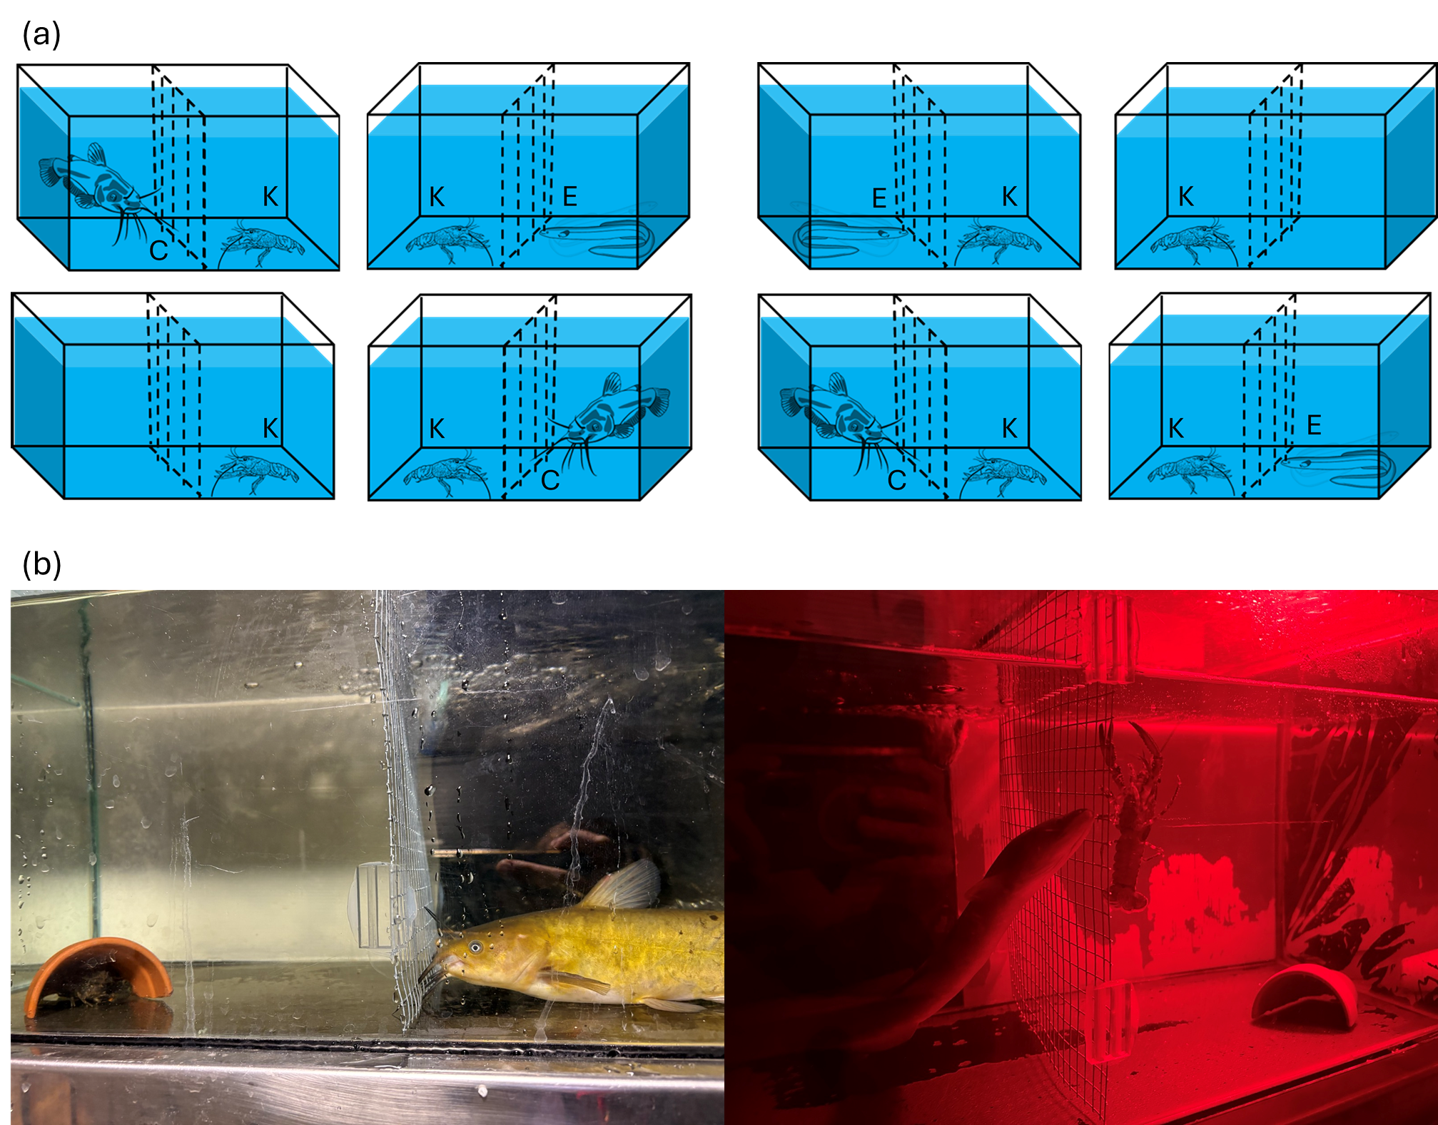
\includegraphics[width=0.8\linewidth,height=\textheight,keepaspectratio]{images/setup_combined.png}

}

\caption{\label{fig-aquarium-setup}(a) Aquarium layout for kōura refuge
seeking behaviour experiment. Each experimental round consisted of eight
aquaria run simultaneously. Each tank contained a single kōura (K) and
refuge (half terracotta plant pot) on one side of a mesh divider. On the
other side was either a single catfish (C), eel (E) or a control with no
fish. The mesh divider allowed visual and chemical cues while preventing
direct physical contact between tank occupants. (b) Experiments were
repeated in light and dark (red light), with photographs showing a
catfish in the light regime (left) and and an eel in the dark regime
(red light) (right) separated from kōura by mesh dividers.}

\end{figure}%

At the beginning of each experiment, an individual kōura was placed in
the middle of the tank compartment containing the refuge. Kōura location
was recorded at 21-time intervals over a 5-hour period, with
observations spaced at progressively longer intervals to capture
immediate behavioural responses at key timepoints (predator introduction
at 60 min, removal at 240 min). The 0-minute recording was the
individual's initial immediate location after its addition to the tank.
Kōura location was recorded as either refuge (the animal was using the
refuge, being inside it or immediately behind it and touching it) or
non-refuge/ in the open (any other location in the tank where the animal
was not in the refuge or touching the refuge). The control tanks had no
fish added but at 60 minutes and again at 240 minutes, the water in the
`predator' compartment was mechanically disturbed by agitating the water
with a small hand net for approximately 30 seconds. This was to simulate
the disturbance time associated with adding and removing fish in the
other treatments with the same size hand net. At the end of each
experiment, the kōura was removed after the final 300-minute
observation.

\subsection{Feeding experiment}\label{feeding-experiment}

Experiments were conducted in glass tanks (320 × 170 × 170 mm),
containing 5 L dechlorinated tap water and a halved terracotta pot (90
mm diameter × 90 mm depth). Catfish and eels had been held at the same
density in separate identical holding tanks for a week prior to
experiment. Fish exudates were collected by placing four fish (catfish
or eel) in a 10 L bucket filled with water from the holding tanks for 15
minutes to concentrate the kairomones in the water. For eel and catfish
treatments, 1 L from the buckets was added to each tank already holding
5 L of tap water, and for control an additional 1 L of dechlorinated tap
water was added. Next, 10 Hikari Tropical carnivore pellets were added
to each tank. Experimental trials showed pellets remain intact in tap
water for over 24 hours. In three rounds, a total of 46 male kōura were
measured and weighed. Their mean (± SD) OCL was 27.93 mm (± 4.80), with
a range of 20.48 to 40.88 mm, and the mean (± SD) wet weight of 15.83 g
(± 8.99), ranging from 6.00 to 42.00 g. Each kōura was then placed
individually in a tank. To investigate how starvation period influenced
feeding motivation, each round kōura were starved for different periods
(either 0, 3 or 4 days) prior to the feeding experiment. After 0 days
starvation, 14 kōura were exposed to eel water (n = 4), catfish water (n
= 6) or control water (n = 4). After 3 days starvation, 16 kōura were
exposed to eel water (n = 6), catfish water (n = 5) or control water (n
= 5). After 4 days starvation, 16 kōura were exposed to eel water (n =
5), catfish water (n = 5) or control water (n = 6). After 24 hours, when
each experiment was terminated, the number of pellets eaten (to the
nearest quarter pellet) was counted and the feeding rate (pellets eaten
per gram of wet weight (WW) of kōura) calculated.

\subsection{Data analysis}\label{data-analysis}

To analyse kōura refuge use, beta-binomial generalized linear
mixed-effects models (GLMMs) were fitted using the glmmTMB package in R
(Brooks et al. 2017; R Core Team 2025). To address potential
non-independence of repeated observations within tanks, raw observations
were first aggregated into three experimental periods (before, during,
and after predator introduction) per individual kōura, with the number
of observations in refuge out of total observations per period used as
the response variable. Treatment (catfish, eel, control) and period
(before, during, after) were included as fixed effects, and tank and
experimental round as random intercepts. Because light condition and
experimental round were fully confounded by design (rounds 1--4 in
light, rounds 5--8 in darkness), separate analyses were conducted for
each light condition to allow round as a random intercept and to test
whether treatment effects varied under each light condition. A
beta-binomial distribution was used to account for overdispersion in the
binomial proportion data. Model fit was assessed using DHARMa
simulation-based residuals, including tests for overdispersion and
zero-inflation ({Hartig et al.} 2024). Marginal means and pairwise
contrasts between factor levels were obtained using the emmeans package
(Lenth et al. 2026), with p-values adjusted for multiple comparisons
using Sidak correction. Additionally, a combined GLMM (without round as
random effect) was fitted to test the overall effect of light condition
across all treatments. Spearman rank correlations with
Bonferroni-adjusted p-values were used to investigate potential
relationships between kōura body size (OCL) and overall refuge use (all
time intervals combined) in the three treatments.

Kōura feeding rate was analysed using a linear mixed model with pellets
consumed per gram wet weight as the response variable and starvation
period (0, 3, 4) as a fixed effect, with tank identity as a random
intercept to account for potential tank-level clustering. Because each
starvation period was conducted in a separate experimental round,
starvation period and experimental round were fully confounded by
design. Consequently, round was excluded as a random effect. However,
starvation period was included as a fixed effect to test for differences
in feeding across hunger states, acknowledging that observed effects may
reflect round-specific variation rather than hunger alone. Model
selection using AICc indicated that starvation period alone provided the
best fit, with treatment not improving model fit (delta AICc = 14.38).
Therefore, treatment effects were excluded from the main model and
instead examined separately within each starvation period using
stratified linear models to avoid confounding treatment comparisons with
the starvation-round confounding. Model assumptions were verified using
residual diagnostics (Q-Q plots and residual plots) and testing
normality of residuals using the Shapiro-Wilk test. As residuals at day
0 starvation violated normality assumptions (\emph{p} = 0.011), a
non-parametric Kruskal-Wallis test was executed. Pairwise comparisons
for starvation period were conducted using estimated marginal means with
Sidak adjustment for multiple comparisons.

\section{Results}\label{results}

\subsection{Refuge experiment}\label{refuge-experiment-1}

The proportion of time kōura spent in refuge varied across treatments,
experimental periods, and light conditions
(Figure~\ref{fig-emmeans-stratified}). Stratified analyses revealed that
treatment effects on refuge use differed between light and dark
conditions. Under dark condition, kōura exposed to catfish used refuge
significantly more than those exposed to eels (\emph{p} = 0.004;
Table~\ref{tbl-emmeans-stratified}), however the control treatment in
the dark was not significant with either the catfish or the eel
treatment (\emph{p} = 0.083, \emph{p} = 0.565). In contrast, under light
conditions, there were no significant differences in refuge use between
the three treatments, but refuge use differed significantly between
experimental periods, with lower refuge use before predator introduction
compared to after predator removal (\emph{p} = 0.021). No significant
period effects were observed in dark conditions. The combined model
showed that light regime had a significant effect on refuge use
(\emph{p} = 0.005), with kōura using refuge more in light than in dark
conditions across all treatments. Overall, under light conditions, the
pattern of refuge use in the control treatment was more similar to the
catfish treatment, whereas under dark conditions it more resembled the
eel treatment (Fig. 3; Table S1). There was also no relationship between
kōura OCL and refuge use in any of the three treatments (rs = -0.09,
\emph{p} = 0.693, rs = 0.09, \emph{p} = 0.680 and rs = 0.16, \emph{p} =
0.494 for catfish, eel and control treatments respectively, all NS).

\begin{figure}

\centering{

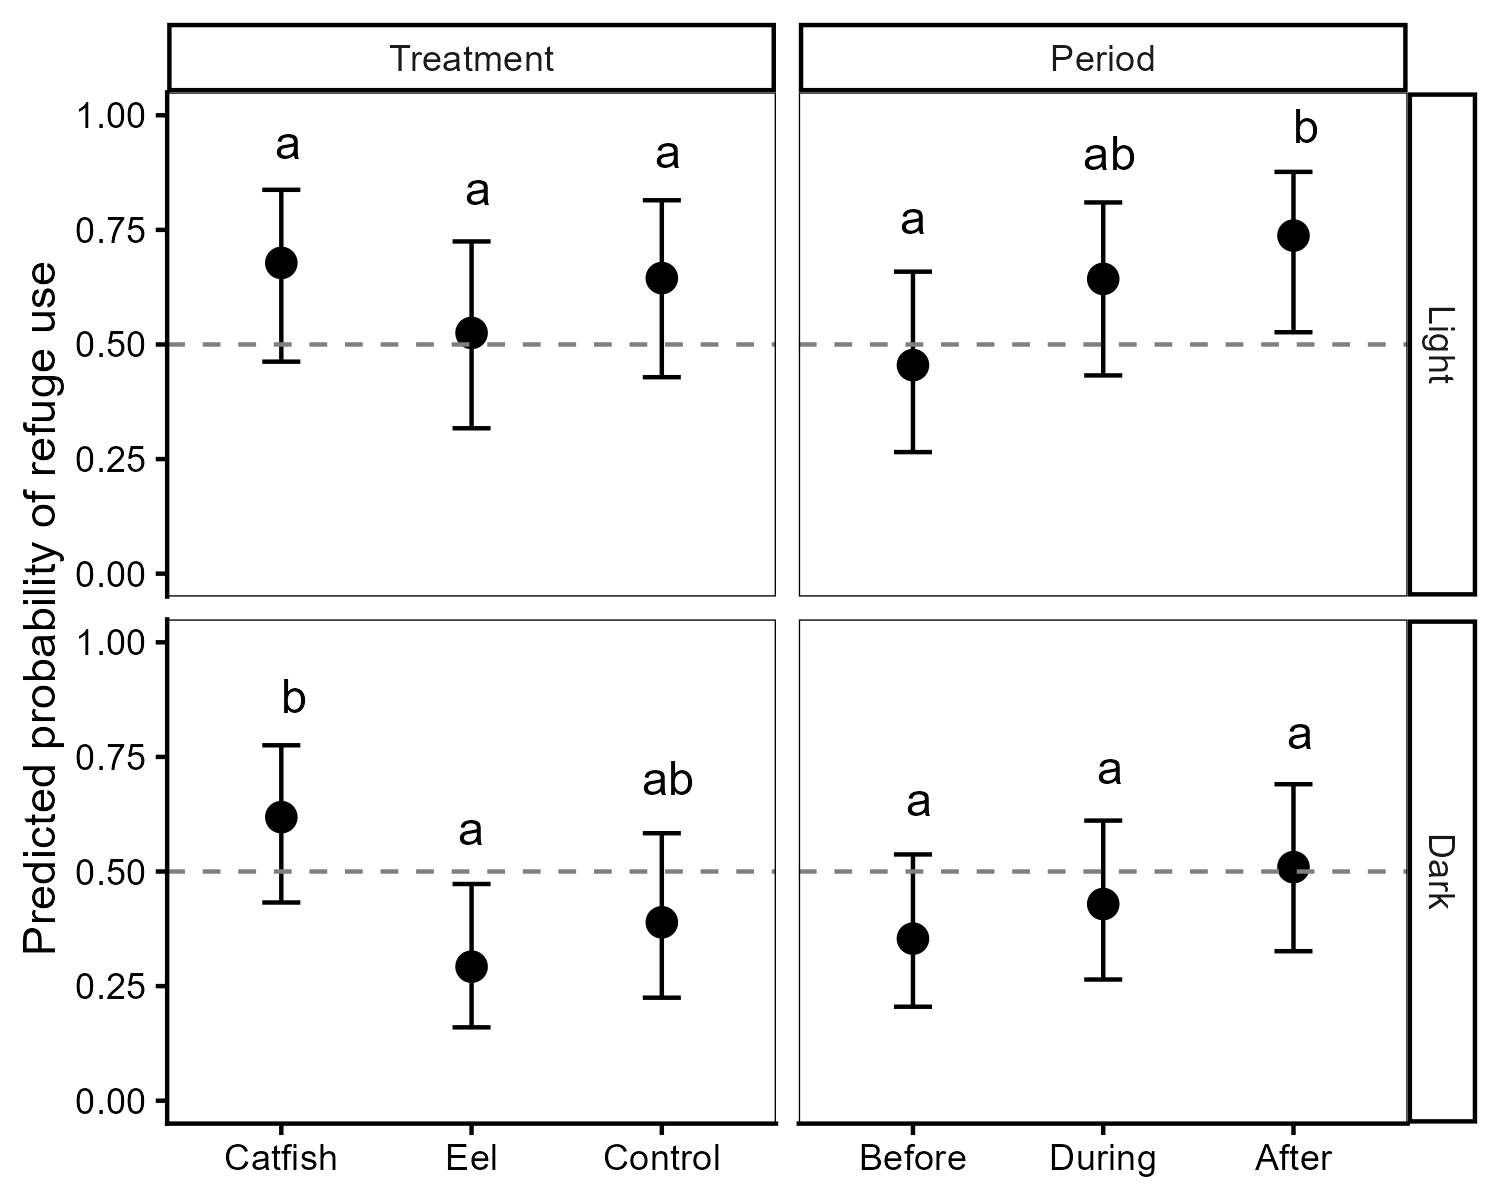
\includegraphics[width=0.65\linewidth,height=\textheight,keepaspectratio]{outputs/fig-emmeans-stratified.png}

}

\caption{\label{fig-emmeans-stratified}Predicted marginal probabilities
of refuge use by treatment and experimental period in light and dark
conditions. Results are shown separately for light (top) and dark
(bottom) conditions, each fitted with a beta-binomial GLMM. Points
represent model-estimated marginal means with 95\% confidence intervals
shown as error bars. Different letters (a, b) indicate statistically
significant differences based on Tukey-adjusted pairwise comparisons
within each factor. The dashed line at 0.5 marks the threshold where
kōura spend half their time in refuge.}

\end{figure}%

\begingroup\fontsize{9}{11}\selectfont

\begin{longtable}[t]{llrrrrrr}

\caption{\label{tbl-emmeans-stratified}Pairwise contrasts for kōura
refuge use in light and dark conditions. Results are shown separately
for each light condition from beta-binomial GLMMs. Odds ratios and
p-values are shown for treatment and period comparisons. P-values are
Sidak-adjusted for multiple comparisons within each factor.}

\tabularnewline

\toprule
Condition & Contrast & Odds ratio & SE & df & Null & z value & p value\\
\midrule
\cellcolor{gray!8}{Light} & \cellcolor{gray!8}{control / catfish} & \cellcolor{gray!8}{0.863} & \cellcolor{gray!8}{0.396} & \cellcolor{gray!8}{Inf} & \cellcolor{gray!8}{1} & \cellcolor{gray!8}{-0.322} & \cellcolor{gray!8}{0.944}\\
Light & control / eel & 1.641 & 0.734 & Inf & 1 & 1.108 & 0.509\\
\cellcolor{gray!8}{Light} & \cellcolor{gray!8}{catfish / eel} & \cellcolor{gray!8}{1.903} & \cellcolor{gray!8}{0.866} & \cellcolor{gray!8}{Inf} & \cellcolor{gray!8}{1} & \cellcolor{gray!8}{1.414} & \cellcolor{gray!8}{0.333}\\
Light & before / during & 0.463 & 0.194 & Inf & 1 & -1.836 & 0.158\\
\cellcolor{gray!8}{Light} & \cellcolor{gray!8}{before / after} & \cellcolor{gray!8}{0.297} & \cellcolor{gray!8}{0.135} & \cellcolor{gray!8}{Inf} & \cellcolor{gray!8}{1} & \cellcolor{gray!8}{-2.672} & \cellcolor{gray!8}{0.021}\\
\addlinespace
Light & during / after & 0.641 & 0.294 & Inf & 1 & -0.969 & 0.597\\
\cellcolor{gray!8}{Dark} & \cellcolor{gray!8}{control / catfish} & \cellcolor{gray!8}{0.393} & \cellcolor{gray!8}{0.172} & \cellcolor{gray!8}{Inf} & \cellcolor{gray!8}{1} & \cellcolor{gray!8}{-2.133} & \cellcolor{gray!8}{0.083}\\
Dark & control / eel & 1.542 & 0.655 & Inf & 1 & 1.019 & 0.565\\
\cellcolor{gray!8}{Dark} & \cellcolor{gray!8}{catfish / eel} & \cellcolor{gray!8}{3.924} & \cellcolor{gray!8}{1.693} & \cellcolor{gray!8}{Inf} & \cellcolor{gray!8}{1} & \cellcolor{gray!8}{3.170} & \cellcolor{gray!8}{0.004}\\
Dark & before / during & 0.728 & 0.286 & Inf & 1 & -0.807 & 0.698\\
\addlinespace
\cellcolor{gray!8}{Dark} & \cellcolor{gray!8}{before / after} & \cellcolor{gray!8}{0.527} & \cellcolor{gray!8}{0.215} & \cellcolor{gray!8}{Inf} & \cellcolor{gray!8}{1} & \cellcolor{gray!8}{-1.569} & \cellcolor{gray!8}{0.259}\\
Dark & during / after & 0.723 & 0.290 & Inf & 1 & -0.809 & 0.698\\
\bottomrule

\end{longtable}

\endgroup{}

For all treatments individual kōura were highly variable in their
movement around tanks and use of refuges, even in the time intervals
comprising the first 60 minutes of the experiment, before fish were
introduced. The coefficient of variations (CVs) for kōura refuge use in
the light and the dark before fish introduction were similarly high,
being 60.4 \% and 58.2 \% (both n = 32) respectively, confirming high
baseline variation in kōura refuge use, regardless of treatment type.
Despite this inherent variation in individual kōura behaviour, clear
patterns in kōura refuge use were evident over the course of the
experiment (Figure~\ref{fig-refuge-plot};
{Table~\ref{tbl-refuge-prop}}). Under light conditions, the control
showed the largest overall increase in refuge use (40\% to 82\%), driven
primarily by a sharp rise in the `after' period, while the catfish
treatment showed a more sustained increase across all periods (52\% to
73\%) and the eel treatment the smallest increase (35\% to 53\%). Under
dark conditions, the pattern shifted, with the catfish treatment showing
the greatest increase (39\% to 70\%), while the eel treatment showed a
modest and non-sustained increase (27\% to 41\% during `exposure',
returning to 36\% `after'), and the control remained comparatively low
throughout (37\% to 47\%).

\begin{figure}

\centering{

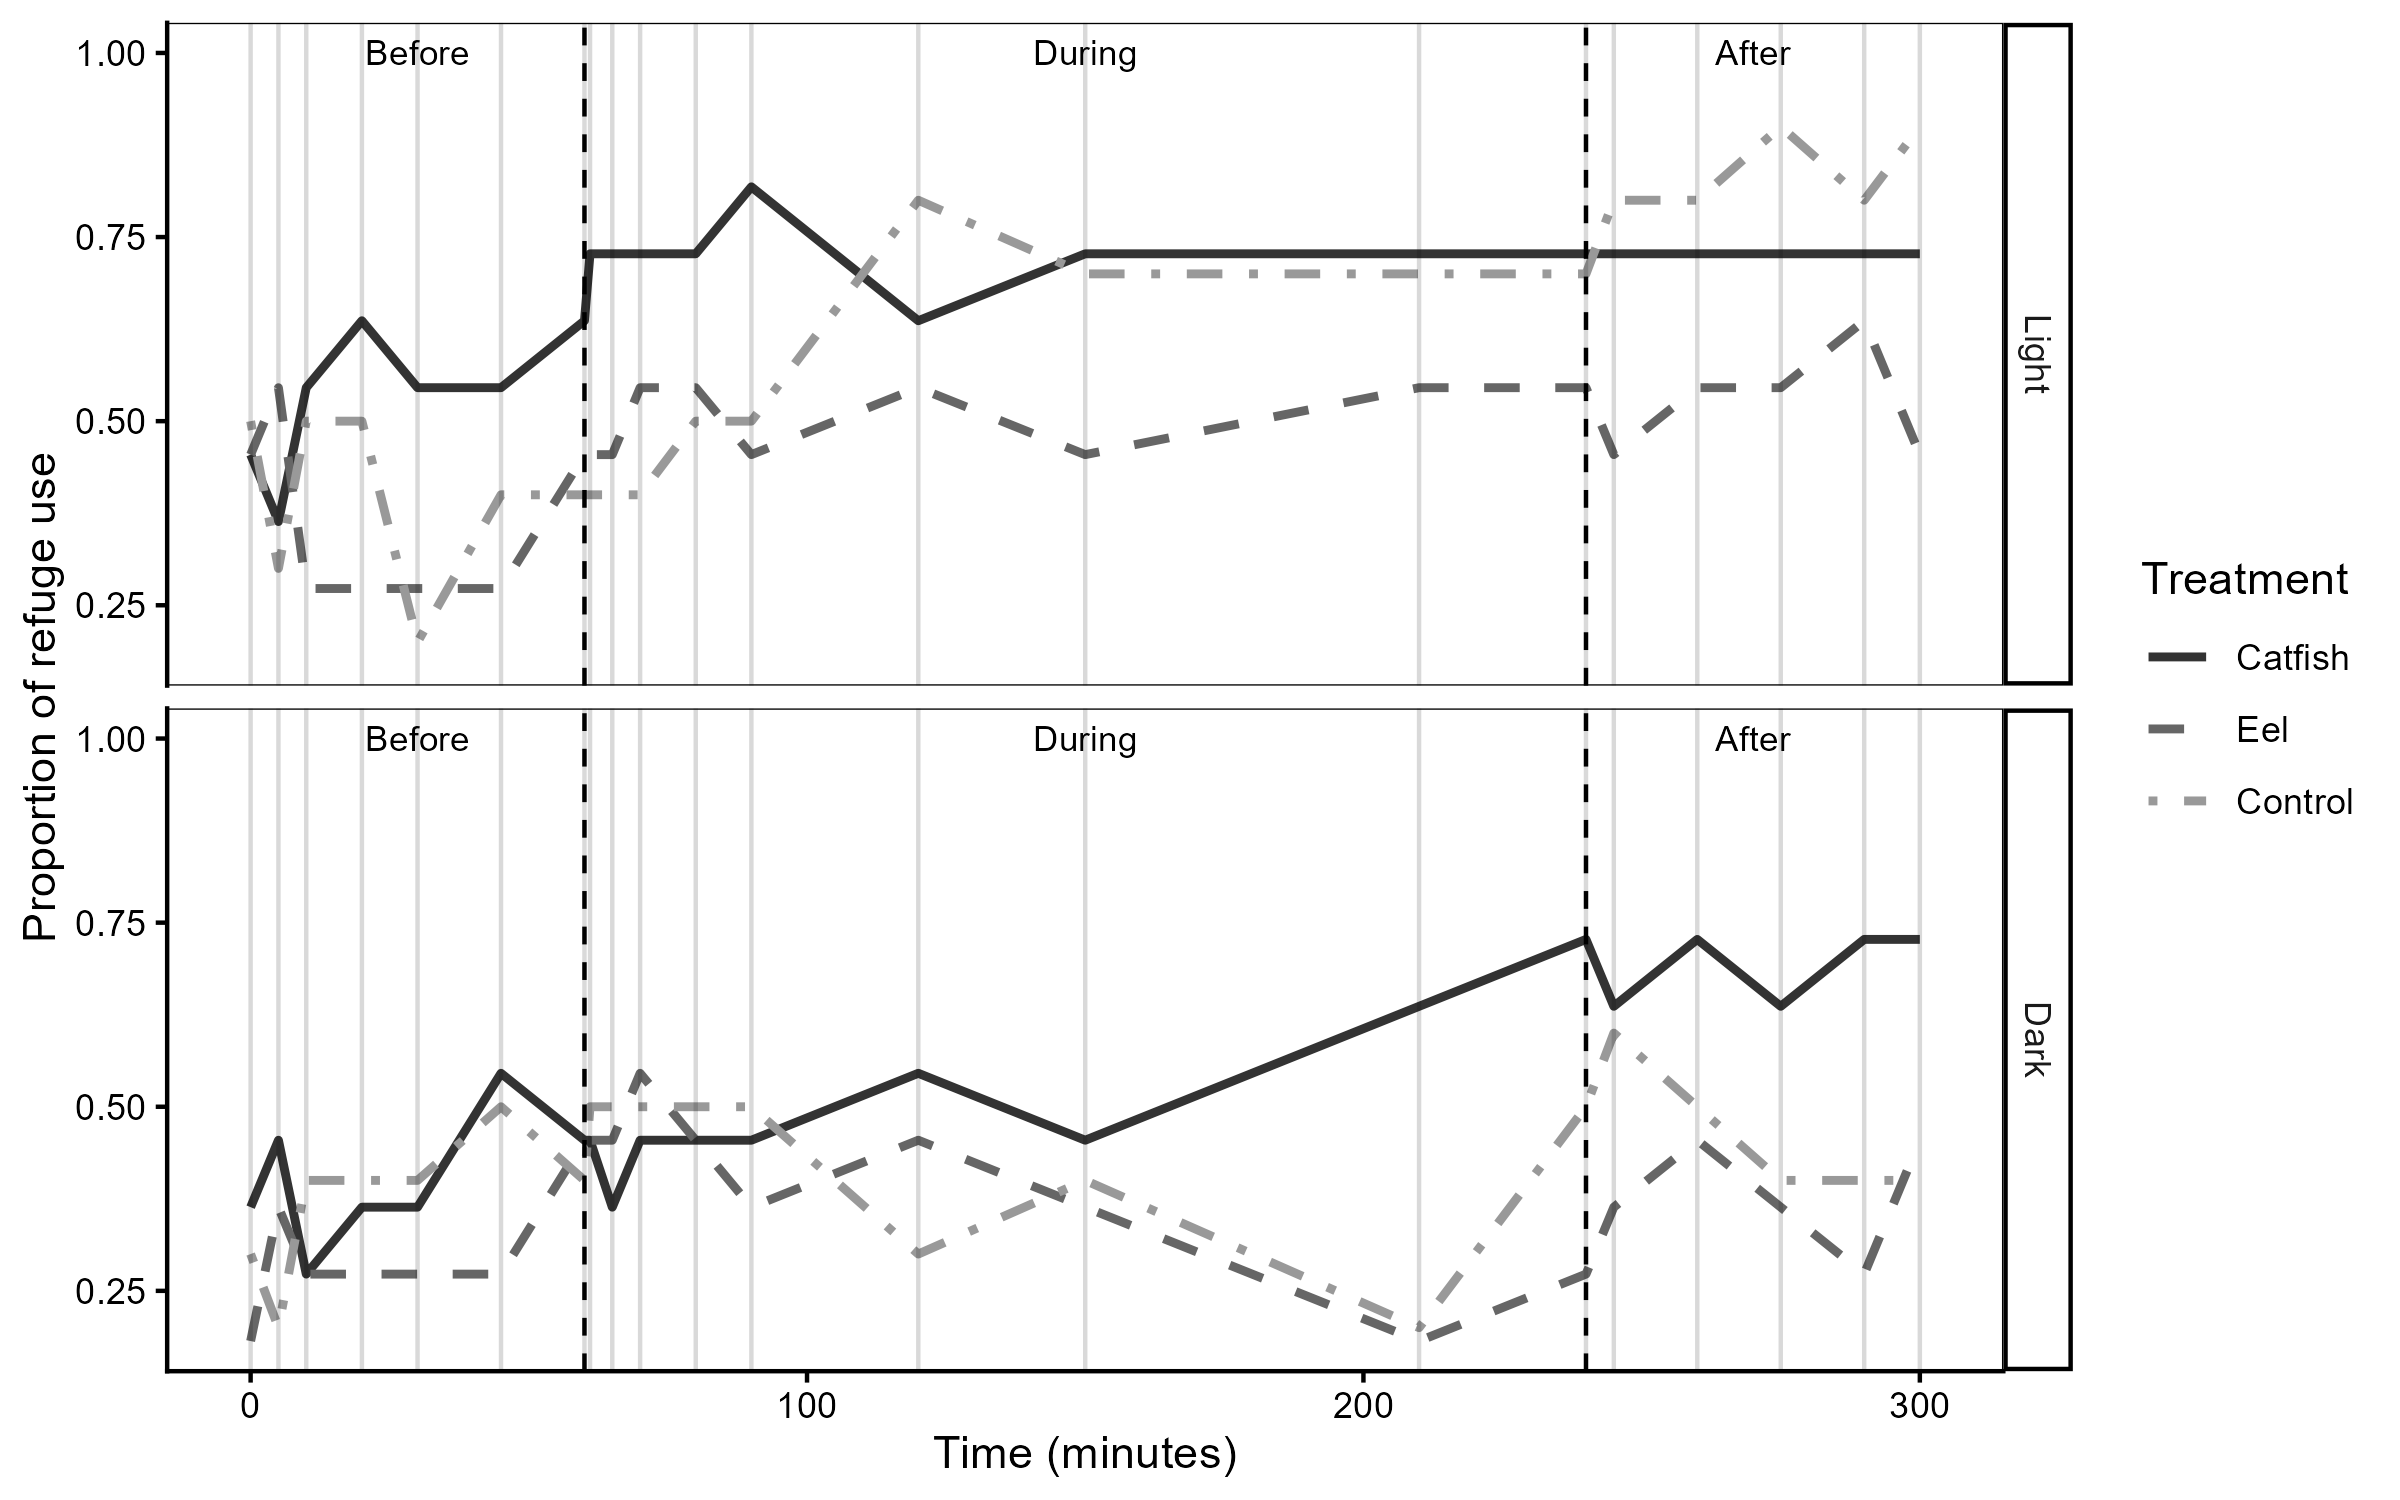
\includegraphics[width=0.8\linewidth,height=\textheight,keepaspectratio]{outputs/fig-refuge-plot.png}

}

\caption{\label{fig-refuge-plot}Kōura refuge use over the course of the
experiment, showing the proportion of time spent in refuge across three
periods (before, during, and after predator exposure) for each treatment
(catfish: dark grey solid line; eel: medium grey dashed line; control:
light grey dot-dash line) under light (top) and dark (bottom)
conditions. Black dashed vertical lines indicate the start and end of
predator exposure and grey vertical lines show individual observation
times.}

\end{figure}%

\subsection{Feeding experiment}\label{feeding-experiment-1}

The linear mixed model showed that starvation period had a significant
effect on kōura feeding rate (3 days: \emph{p} \textless{} 0.001; 4
days: \emph{p} = 0.046; Figure~\ref{fig-feeding-plot};
{Table~\ref{tbl-feeding-summary}}). Treatment was not included in the
main model following model selection. Stratified analyses revealed no
significant treatment effects across starvation periods. Although
residuals at day 0 violated normality (Shapiro-Wilk \emph{p} = 0.0112),
the non-parametric Kruskal-Wallis test confirmed no treatment effect
(\emph{p} = 0.3165). Starvation days 3 and 4 met normality assumptions
and showed no significant treatment effects (\emph{p} = 0.1495 and
0.1573 respectively). After 4 days starvation, the mean (±SE) kōura
feeding rate (pellets g WW\(^{-1}\)) for the control was over two and a
half times that of the catfish and eel treatments (0.148 ± 0.035
compared to 0.059 ± 0.039 and 0.052 ± 0.039 respectively).

\begin{figure}

\centering{

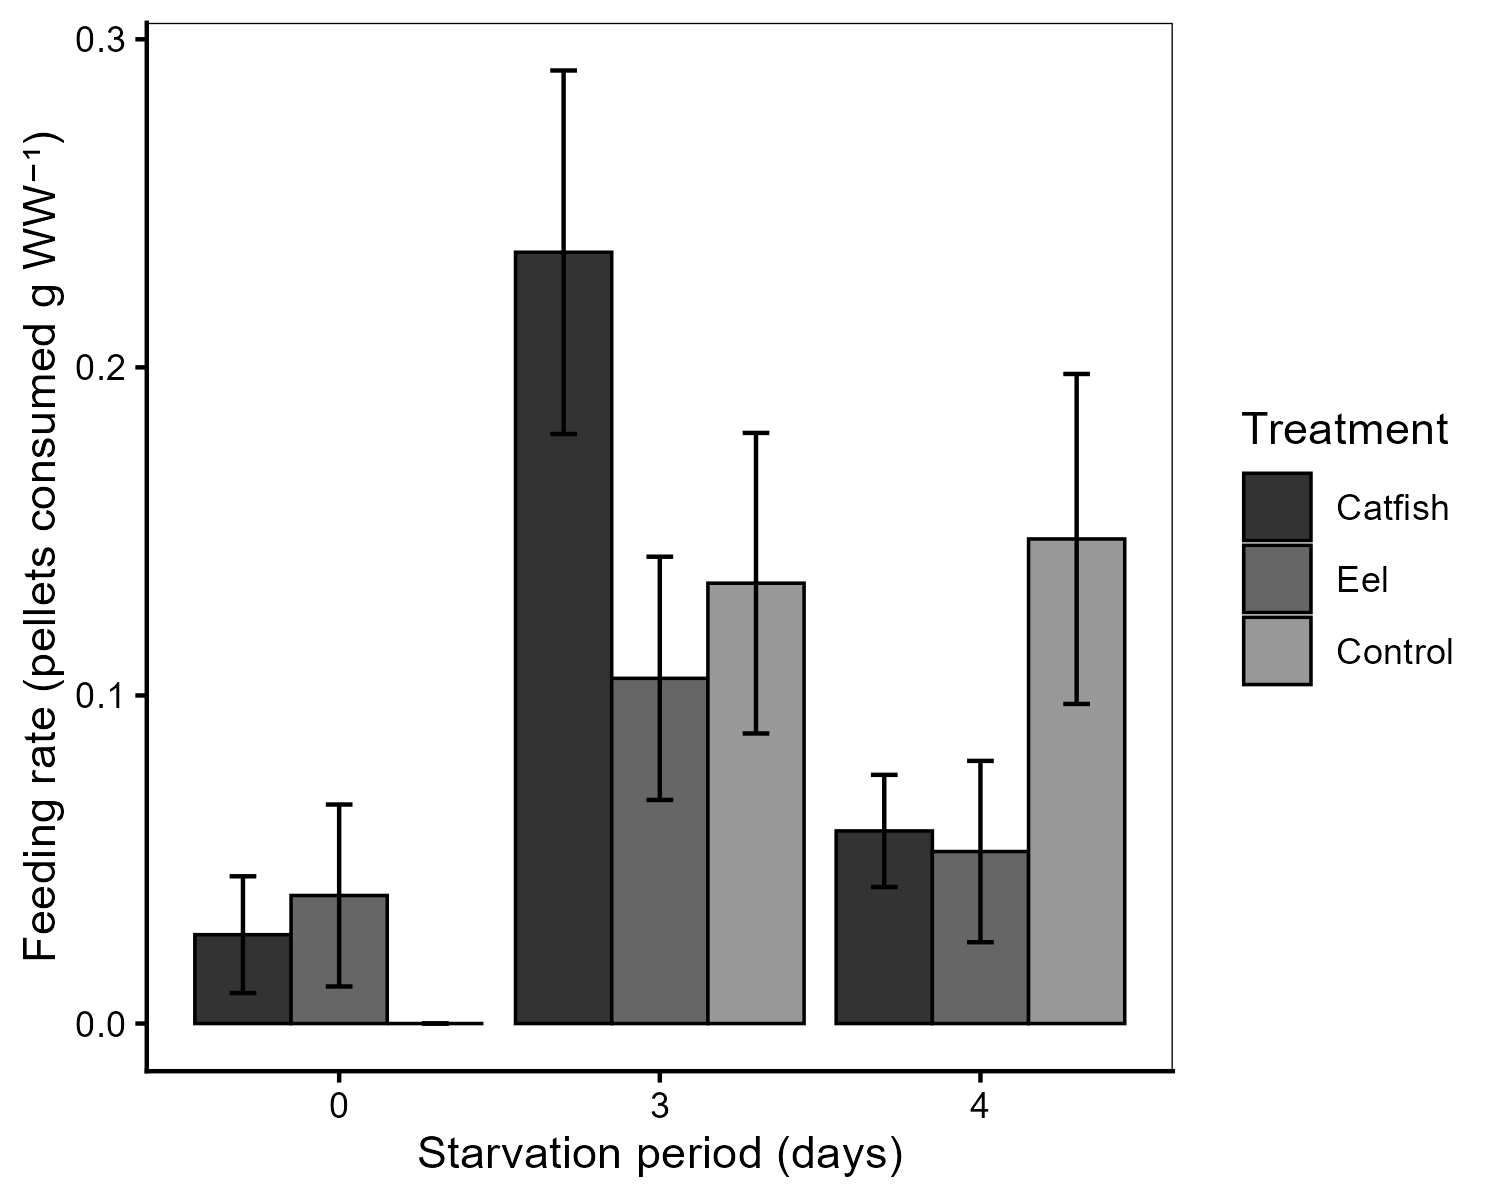
\includegraphics[width=0.65\linewidth,height=\textheight,keepaspectratio]{outputs/fig-feeding-plot.png}

}

\caption{\label{fig-feeding-plot}Mean (±SE) kōura feeding rate (pellets
consumed per gram wet weight kōura) across predator treatments (catfish,
eel, control) and starvation periods (0, 3, and 4 days).}

\end{figure}%

\section{Discussion}\label{discussion}

Prey modify their behaviour in response to predation risk, creating a
`landscape of fear' that affects foraging, movement, and habitat use
independently of actual predation events (Laundré et al. 2001). Our
study adds to a growing body of literature (i.e., (Sniegula et al.
2025)) showing invasive predators can generate stronger NCEs on native
prey than native predators, with potentially far-reaching consequences
on invaded ecosystems. The results in our experiments suggest the
introduction of a novel predator may change the prey's fear landscape in
ways that a native predator does not. Kōura are a keystone species that
act as ecosystem engineers in Aotearoa freshwaters, meaning that
predator-induced changed in kōura behaviour may indirectly affect
ecosystem-level properties (e.g., resources or other species) through
non-consumptive pathways (Peacor and Werner 2001). Such indirect effects
represent a form of behavioural trophic cascade (Schmitz et al. 1997),
whereby predator presence alone drives ecosystem-level change. Our
results also highlight that prey naivety does not necessarily manifest
as a failure to respond to novel predators. Instead, naïve prey may
exhibit an over-avoiding response consistent with generalisation theory
(Sih et al. 2010; Ehlman et al. 2019), which potentially has important
implications for predicting the ecological impacts of invasive species.

\subsection{Refuge use}\label{refuge-use}

Under dark conditions, kōura demonstrated greater refuge-seeking
behaviour when exposed to the novel catfish than to native eel. This
result is notable because it contradicts the classic prey naivety
hypothesis, which predicts that prey underestimate or fail to
appropriately respond to novel predators due to a lack of shared
evolutionary history (Carthey and Banks 2014). Instead, kōura seemingly
exhibited an enhanced defensive response to the novel predator. Such
over-responses to unfamiliar predators are less commonly reported but
are consistent with fear generalisation theory, whereby experience with
native predators primes a generalised heightened vigilance response to
any unfamiliar threat (Ehlman et al. 2019; Sih et al. 2023). For naïve
prey, unfamiliar cues could trigger such a response because the
consequences of ignoring a potential predation threat could be fatal,
even when, in reality, the actual predation risk is absent (Dawkins and
Krebs 1979; Lima and Dill 1990). Such generalised responses are often
overcautious and energetically costly because prey may initially treat
uncertain threats as highly dangerous until further experience is
acquired (Sih et al. 2010). Unlike classic prey naivety scenarios where
the novel predator poses no actual threat, catfish genuinely predate
kōura, meaning the heightened refuge response carries a real energetic
cost but is not disproportionate to the actual risk of predation.
Elevated refuge use is itself a meaningful NCE, reducing foraging time
with potential consequences for growth, reproduction, and population
persistence (Preisser et al. 2005; Sheriff et al. 2020). However, this
behaviour may simultaneously confer protection against direct predation
as experimental evidence shows that shelter significantly reduces
catfish predation on crayfish (Adams 2007; Zhao et al. 2024). This
result suggests that enhancing or restoring habitat complexity in
catfish-invaded lakes could mitigate both direct predation and
fear-driven reductions in foraging, though direct field testing is
needed.

Before fish were added to the tanks, refuge use by kōura was similar
across treatments but highly variable at the individual level,
reflecting substantial behavioural variation. The control treatment
showed increasing refuge use over time, particularly under light
conditions, which is unsurprising given that kōura are nocturnally
adapted and need to remain hidden during daylight to avoid visual
predators such as cormorants (Devcich 1979). Importantly, treatment
effects on refuge use depended on light condition. Under dark
conditions, when kōura are naturally more active, catfish exposure
resulted in significantly greater refuge use than eel exposure. Control
refuge use was intermediate between the two predator treatments, though
the reasons for this pattern are unclear from the current data. The
contrasting responses of kōura to catfish and eels indicates
biologically meaningful differences in NCE between exposure to a novel
and native predator.

Unlike the response when exposed to catfish, kōura reduced their refuge
use in the presence of eels. This contrasting response likely reflects
the long evolutionary relationship between kōura and eels, though the
strength of coevolutionary adaptation in these specific lakes remains
uncertain. The lakes naturally have restricted access to the coast
limiting the number of eels present and historical vulcanism has
affected these dynamics with a potential historical separation
approximately 700 years ago following the Kaharoa eruption
(\textasciitilde AD 1314; (Hogg et al. 2003)). Nevertheless, kōura
probably were able to recognise chemical and visual cues from the eels
and respond in a proportionate rather than precautionary way (Shave et
al. 1994). Instead of hiding, kōura may rely on contextual information,
such as predator size, movement patterns, or chemical concentrations, to
modulate their response (Wood and Moore 2020b). This calibrated response
makes ecological sense as longfin eels are the most widely distributed
fish in the freshwaters of Aotearoa (McDowall 1990), and a persistent
high-intensity refuge response to eels would likely impose substantial
foraging costs. Whether shaped by deep coevolutionary history or by
recognition of eels as an established native predator, kōura show a
nuanced, context-dependent response to eels rather than an
over-generalised avoidance strategy. This pattern was most pronounced in
the dark conditions, where kōura refuge use in all three treatments
began similarly but changed progressively over the course of the
experiment. Kōura in the catfish treatment steadily increased their
refuge use, while kōura in the eel treatment showed similar behaviour to
those in the control treatment, with decreases to baseline levels by the
end of the observation period. This result suggests that under
conditions most relevant to natural activity by kōura, chemical
recognition of the familiar eel predator is sufficient to enable a
calibrated, low-cost response, while the unfamiliar catfish continues to
elicit sustained precautionary refuge use (Shave et al. 1994; Wood and
Moore 2020a). Beyond predator recognition, the reduced refuge use
observed in eel-exposed kōura may not reflect a lack of response but
could instead represent active escape-searching behaviour (i.e.~a
``flight'' response). If this was the behavioural motivation, kōura
would be attempting to move away from an area where they perceived
themselves as vulnerable in the confined tank space, rather than
retreating to a refuge where they might be prone to a known predator.

\subsection{Feeding behaviour}\label{feeding-behaviour}

NCEs are not a single process but emerge from the interaction between
sensory ecology and environmental context. The absence of a kairomone
effect on feeding in this study likely reflects a combination of
methodological constraints rather than an absence of NCEs on foraging
behaviour. The feeding experiment, in which predators were presented
solely through chemical cues without visual information, did not
demonstrate a clear fish predator NCE on kōura. This may have been due
to the concentration of predator kairomones not being high enough to
exceed detection thresholds (Brown et al. 2004), the starvation
conditions during the experiment, the restricted time frame of the
experiment, or a combination of these factors. Kōura can readily detect
necrotic fish tissue and readily leave refuges to scavenge on catfish,
eel, and marine fish carcasses with little discrimination between fish
species, indicating that chemosensory responses in kōura may depend on
cue type, context, and concentration rather than predator identity alone
(MacNeil et al. 2025). The concentration of live fish exudates in our
experiment relative to natural conditions is difficult to determine,
while kairomones were concentrated by confining fish in a bucket, in our
experimental tanks they were subsequently diluted in 5 L of water, not
replenished, and potentially degraded over the 24-hour period. Whether
the resulting concentration reflects, exceeds or falls below
ecologically relevant levels in lakes where kōura and predators coexist
remains unclear, and future studies should attempt to quantify natural
kairomone concentrations to better calibrate experimental designs
(Achtymichuk et al. 2025). In addition, many crayfishes show a stronger
response to alarm cues of conspecifics (Stebbing et al. 2010; Gherardi
et al. 2011; Ramberg-Pihl and Yurewicz 2020), and to kairomones from
predators on a conspecifics diet (Beattie and Moore 2018). Fish
predators in our experiments were maintained on the same diet as kōura
for an extended acclimation period prior to exposure (see Methods),
which may have further dampened or negated the threat signals received
from kairomones (Smee and Weissburg 2006). Furthermore, the
pre-experiment starvation period for kōura may have been insufficient to
elicit a very strong feeding response, as crayfish such as kōura are
opportunistic foragers which are necessarily adapted to going for
prolonged periods without feeding (Hazlett 2003). The length of time
since feeding can influence foraging behaviour, with previous studies
indicating that crayfish will be more active foragers after being
starved for at least three days (Hazlett 2003). In the current study,
the longest starvation period was four days and at this point there was
a clear discrepancy between the control feeding rate and the much lower
feeding rates in the two fish treatments. Allowing for ethics and
welfare concerns, if we had extended the starvation period, this may
have elicited a stronger and prolonged response. Additionally, the
stress of confinement in an artificial setting may itself have altered
normal kōura feeding responses, as elevated baseline stress hormones are
known to modify foraging behaviour independently of predator cue
exposure (Clinchy et al. 2012). Finally, feeding was measured as a
single endpoint after 24 hours, providing no information on whether
kōura initially suppressed feeding after kairomone exposure before
eventually resuming normal feeding activity (Wright et al. 2010).
Further experiments using higher kairomone concentrations, longer
starvation periods, and continuous feeding monitoring would help clarify
whether non-visual predator cues generate NCEs on kōura foraging
behaviour.

\subsection{Conclusions}\label{conclusions}

As ecosystems become increasingly novel under global change, the
reliability of historical predator--prey cues may decline, amplifying
behavioural mismatches (Sih et al. 2011). The present study provides
experimental evidence that invasive brown bullhead catfish have the
potential to exert stronger NCEs on kōura, an endemic freshwater
crayfish when compared to their native predator, the longfin eel. The
heightened refuge-seeking response to catfish likely reflects a
generalised antipredator response triggered by unfamiliar chemical and
visual cues, consistent with a fear generalisation framework. In
contrast, the reduced response to eels suggests that familiarity with
native predators enables kōura to make more proportionate risk
assessments, although their behaviour may have also been an antipredator
strategy. Future studies should particularly include kōura from
eel-inhabited waterways, which would determine whether populations with
a recent coevolutionary history with native eels display similar
proportionate responses, thereby confirming whether the patterns
observed here reflect broader adaptive differences across kōura
populations with distinct predatory histories. Additionally, comparative
studies of kōura sourced from catfish-invaded versus catfish-free
catchments would be worthwhile to assess whether repeated exposure over
multiple generations has resulted in rapid evolution or behavioural
plasticity in antipredator responses, and whether catfish-experienced
kōura show more calibrated responses to catfish presence than naïve
kōura. Such evolutionary dynamics could have important implications for
predicting kōura persistence in catfish-invaded systems (Sih et al.
2010). From a management perspective, translocation of kōura from
catfish-experienced source populations into catchments facing imminent
catfish invasion may represent a more feasible strategy for seeding
populations with individuals capable of more adaptive responses.
Although we found no significant NCE of fish exudates on feeding
behaviour, our study suggests further investigations of non-visual
predator cues on kōura foraging behaviour is warranted. Because kōura
are a keystone species that ecosystem engineer, even a small increase in
refuge use driven by catfish presence could have cascading effects on
sediment dynamics, decomposition, and nutrient cycling in invaded lakes.
As brown bullhead catfish continue to spread across Aotearoa's rivers
and lakes, management strategies aimed at protecting kōura should
account for the behavioural cost of catfish NCEs alongside direct
predation pressure as an underappreciated and ecologically significant
dimension to this invasion.

\section{Acknowledgements}\label{acknowledgements-1}

We thank Te Arawa Lakes Trust and Te Komiti Whakahaere for the
opportunity to collect and study the treasured kōura. We are grateful to
Soweeta Fort-D'ath and William Anaru (Te Arawa Lakes Trust), and Tihini
Grant (Ngāti Pikiao). We also thank Nick Ling and Ben Roche (University
of Waikato) for assisting with catfish and eel collection.

\clearpage
\providecommand{\chaptermark}[1]{}
\ifcsname c@chapter\endcsname
\setcounter{chapter}{3}
\setcounter{figure}{0}
\setcounter{table}{0}
\setcounter{section}{0}
\addcontentsline{toc}{chapter}{\protect\numberline{3}Where do K\={o}ura Live?}
\chaptermark{Where do K\={o}ura Live?}
\fi
\providecommand{\thechapter}{3}
\thispagestyle{empty}
\begin{tikzpicture}[remember picture, overlay]
  \begin{scope}
    \clip ([yshift=-7cm]current page.north west)
          rectangle ([yshift=4.5cm]current page.south east);
    \node[inner sep=0pt, anchor=north]
      at ([yshift=-7cm]current page.north)
      {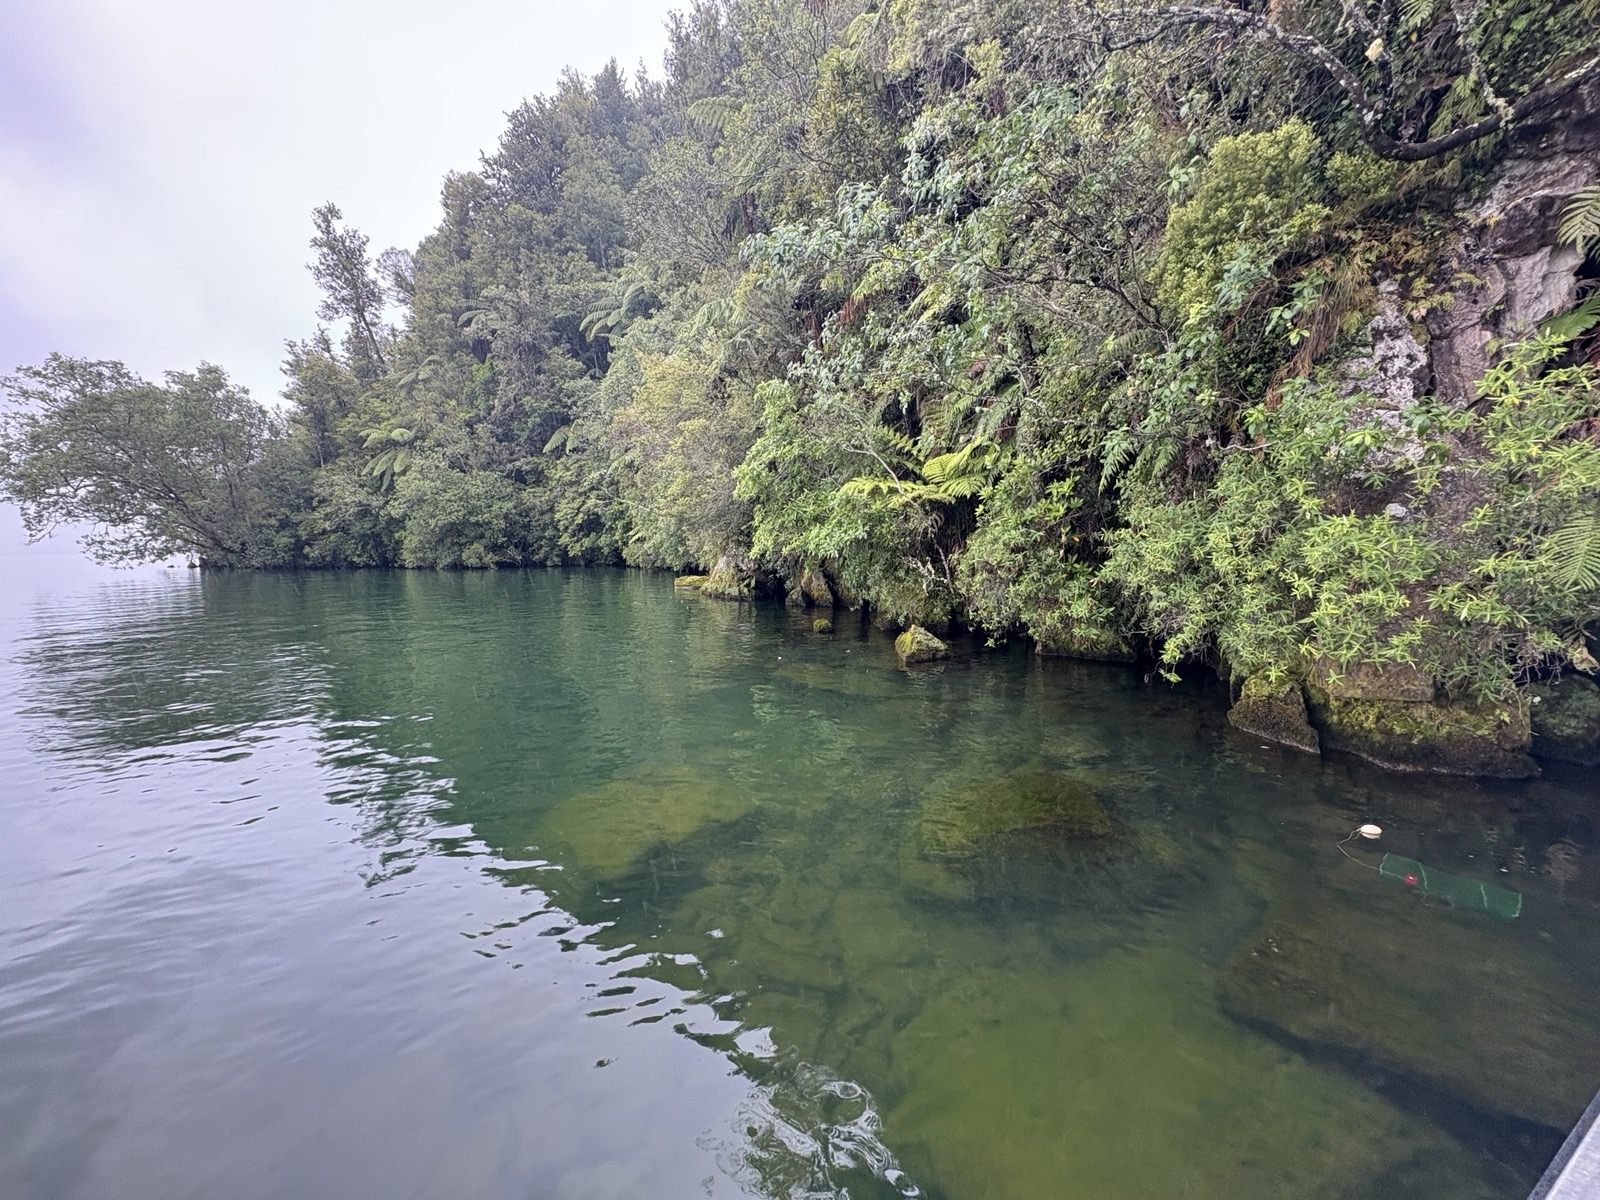
\includegraphics[height=18.2cm]{images/ch3_cover.jpg}};
  \end{scope}
  \fill[black]
    (current page.north west) rectangle ([yshift=-7cm]current page.north east);
  \node[color=thesissand, align=left,
        font=\fontsize{13}{16}\selectfont\sffamily, anchor=west]
    at ([xshift=1.5cm, yshift=-1.5cm]current page.north west)
    {Chapter \thechapter};
  \node[color=white, text width=0.85\paperwidth, align=left,
        font=\fontsize{22}{28}\selectfont\bfseries\sffamily, anchor=west]
    at ([xshift=1.5cm, yshift=-4cm]current page.north west)
    {Where do K\={o}ura Live?};
  \node[color=white, text width=0.85\paperwidth, align=left,
        font=\fontsize{10}{13}\selectfont\itshape\sffamily, anchor=north west]
    at ([xshift=1.5cm, yshift=-5.0cm]current page.north west)
    {Littoral habitat structure influences freshwater crayfish populations in five volcanic lakes of Aotearoa New Zealand};
  \fill[black]
    (current page.south west) rectangle ([yshift=4.5cm]current page.south east);
  \node[color=white, text width=0.85\paperwidth, align=left,
        font=\fontsize{9}{13}\selectfont\sffamily, anchor=west]
    at ([xshift=1.5cm, yshift=3.2cm]current page.south west)
    {Olivier V.\ Raven, Francis J.\ Burdon, Ian A.\ K.\ Kusabs, Robin Holmes \& Deniz Özkundakci};
  \node[color=thesissand, text width=0.85\paperwidth, align=left,
        font=\fontsize{9}{13}\selectfont\itshape\sffamily, anchor=west]
    at ([xshift=1.5cm, yshift=1.5cm]current page.south west)
    {Hydrobiologia (2026) --- https://doi.org/10.1007/s10750-026-06302-z};
\end{tikzpicture}
\null
\clearpage

\section*{Abstract}\label{abstract-2}
\addcontentsline{toc}{section}{Abstract}

Freshwater crayfish are increasingly threatened by habitat degradation,
declining water quality, and invasive species. In Aotearoa New Zealand,
lake populations of the endemic northern freshwater crayfish
\emph{Paranephrops planifrons} (kōura) have declined by up to 91 \%.
Identifying key habitat requirements is essential to improve the
conservation of crayfish facing multiple threats. To assess littoral
habitat associations, we surveyed shoreline habitats in five Aotearoa
lakes and modelled kōura occupancy, abundance, and biomass using
generalised additive mixed models. Kōura occupancy increased with
shoreline habitat complexity, particularly coarser substrate types and
greater riparian vegetation cover. Elevated summer surface water
temperatures were negatively associated with kōura occupancy and
abundance, indicating reduced habitat suitability during warm periods.
pH was positively correlated with kōura abundance and biomass. Our
results suggest that the composition and physical structure of littoral
habitats are important drivers of kōura distribution and abundance. As
climatic drivers resulting in warmer water temperatures and reduced
dissolved oxygen are difficult to manage, targeted protection and
restoration of coarse substrate shoreline habitats may provide a
practical conservation response.

\section{Introduction}\label{introduction-1}

Freshwater crayfish (Astacidea) play a vital role in freshwater
ecosystems (Momot 1995). They are ecosystem engineers, exerting
substantial influence over key ecological processes, including nutrient
cycling, organic matter decomposition and bioturbation (Momot 1995;
Collier et al. 1997; Parkyn et al. 2001). They are keystone species due
to their broad trophic niche as predators and detritivores, and their
ability to modify habitats through sediment excavation for burrow
construction, removal of macrophytes, and alteration of
macroinvertebrate communities (Statzner et al. 2003; Creed and Reed
2004; Usio and Townsend 2004; Albertson and Daniels 2018). Nearly
one-third of the world's crayfish species are currently threatened with
extinction (Richman et al. 2015). Despite their ecological importance
and imperilled status, crayfish are frequently overlooked in restoration
and conservation initiatives (Taylor et al. 2019; Danilović et al.
2022).

In Aotearoa New Zealand (hereafter Aotearoa), the endemic northern
freshwater crayfish \emph{Paranephrops planifrons} White, 1842, also
known by its Māori name kōura, inhabits a wide range of freshwater
environments, including rivers, streams and lakes across both main
islands (Hopkins 1970). Beyond its ecological role, kōura hold deep
cultural significance, having historically been an important food source
and trade commodity for iwi (Māori communities; (Hiroa 1921; Kusabs and
Quinn 2009)). However, kōura populations are increasingly threatened by
climate change, invasive species and declining water quality (Kusabs et
al. 2015a; Lee et al. 2025). These declines are likely the result of
multiple interacting environmental stressors, including declining water
quality, deoxygenation and the introduction and consequent impacts of
non-native species (Kusabs and Quinn 2009). For example, in Lakes
Rotorua and Rotoiti, located in the Bay of Plenty region of Aotearoa's
North Island, kōura populations have declined by 76 \% and 91 \%,
respectively, over the past two decades (Kusabs et al. 2026).

In 2016, the invasive North American brown bullhead catfish
(\emph{Ameiurus nebulosus} Lesueur, 1819) was confirmed to be present in
Lakes Rotorua and Rotoiti (Grayling 2020), where it now occurs in large
numbers and preys heavily on kōura (Francis 2019; Kusabs et al. 2026).
To reduce predation risk, kōura typically seek refuge in deeper lake
habitats during the day and migrate to the more productive shallow areas
at night to forage (Devcich 1979). However, summer lake stratification
has led to oxygen depletion in deeper waters, forcing kōura to spend
more time in shallow habitats where predation risk is greater (Dedual
2002). Climate change is expected to intensify these effects by
strengthening thermal stratification and increasing the extent and
duration of anoxic conditions in bottom waters as water temperatures
rise (Woolway et al. 2021; Zhang et al. 2024). In addition, dense beds
of invasive macrophytes may obstruct kōura migration pathways between
deep and shallow habitats (Hessen et al. 2004; Kusabs and Quinn 2009)
and further reduce oxygen availability during seasonal macrophyte
die-off events (Vincent et al. 1984; Hessen et al. 2004; Hamilton et al.
2005).

Declines in kōura populations have cascading ecological impacts and
implications for Māori cultural practices, including reduced
opportunities for customary harvest and disruption of traditional
activities (Kusabs and Quinn 2009; Kusabs et al. 2015a; Kusabs et al.
2026). To effectively conserve and restore populations requires an
improved understanding of where kōura occur within lakes and what
habitats are most important for sustaining healthy populations. Previous
research in stream environments has shown that kōura preferentially
occupy structurally complex habitats characterised by bank undercuts,
woody debris, leaf litter, boulders and low flow velocities (Usio and
Townsend 2000; Parkyn and Collier 2004; Jowett et al. 2008; Parkyn et
al. 2009). In contrast, habitats used by kōura in lakes remains poorly
understood, with previous studies largely focussed on deeper offshore
habitats (Devcich 1979; Kusabs and Quinn 2009; Kusabs et al. 2015b).
These studies suggest that benthic substrate characteristics may be more
important than nutrient enrichment or predator abundance ---
specifically non-native rainbow trout (\emph{Oncorhynchus mykiss}
Walbaum, 1792) --- in determining kōura distribution (Kusabs et al.
2015b). The littoral zone of lakes has received little attention,
despite it being the most productive zone and supporting key life
history processes of kōura (Strayer and Findlay 2010), including
nocturnal foraging and use by ovigerous females prior to juvenile
release (Devcich 1979). Consequently, the littoral zone is likely to
represent an important habitat within lakes for kōura.

In this study, we examine which littoral habitat characteristics are
associated with kōura occurrence, abundance and biomass across five
Rotorua Te Arawa Lakes. We hypothesised that structurally diverse
littoral habitats, including coarse substrates and native macrophytes,
would be positively associated with kōura occurrence and abundance, as
they provide physical refuge and foraging opportunities. Conversely,
invasive submerged macrophytes were expected to have negative
associations with kōura as these dense macrophytes hinder movement and
reduce native biodiversity by displacing native macrophytes, altering
habitat structure, and modifying ecological processes. We further
expected that kōura abundance would be lower in lakes where catfish are
present, as catfish are a known predator on benthic invertebrates and
native fauna. By quantifying these habitat associations within the
littoral zone, this study aims to inform targeted habitat protection and
restoration strategies for the conservation of this culturally and
ecologically important species.

\section{Materials and Methods}\label{materials-and-methods-1}

\subsection{Study location}\label{study-location}

Study sites were selected in five lakes located in the Rotorua Te Arawa
Lakes area in the North Island of Aotearoa. The Lakes Rotorua, Rotoiti,
Rotoehu, Rotomā, and Ōkāreka are located on a warm- temperate volcanic
plateau (280-355 m) where winters are mild and year-round temperatures
typically varies from 4°C to 24°C. The lakes span a wide range of
morphometric and trophic conditions from shallow polymictic eutrophic
systems (Rotoehu, maximum depth 14 m) to deep stratified oligotrophic
lakes (Rotomā, maximum depth 83 m). Shorelines are characterised by a
mix of native riparian vegetation, exotic pasture, and low-density
residential development, with several lakes also supporting stands of
emergent macrophytes. Detailed lake characteristics and shoreline
composition are summarised in Table~\ref{tbl-lake-overview}. All five
lakes have populations of kōura, and brown bullhead catfish was present
in Lakes Rotorua and Rotoiti at time of sampling (Kusabs et al. 2026).

To survey these lakes, a stratified-random survey design was developed.
The entire accessible shoreline of each lake was first mapped using
aerial photos and then ground truthed and classified into dominant
habitat types. Classification used the following criteria: a habitat was
considered dominant ``rocky'' if the combined percentage of bedrock,
boulders, and cobble exceeded 25 \% by surface area; ``sandy'' if sand
was the dominant sediment (≥50 \%) and rocky conditions were not met;
``muddy'' if soft mud or organic matter was dominant and rocky/sandy
conditions were not met; and ``emergent macrophyte'' if emergent native
macrophytes exceeded 25 \% of the shoreline cover by surface area.
Shoreline sites exceeding two meters in depth or classified as
geothermal were excluded, as these conditions were either unsuitable for
kōura or inaccessible for field sampling.

For each lake, the total shoreline length of each habitat type within
this sample frame was calculated in a projected coordinate system (New
Zealand Transverse Mercator 2000; EPSG:2193). To ensure balanced
representation of littoral habitat types across systems and to avoid
confounding lake identity with sampling effort, an equal number of sites
(n = 12) was surveyed in each lake, with sites allocated proportionally
among the dominant shoreline habitat types. All selected sites were
fully accessible for fieldwork, and therefore an oversample was not
required. Within each habitat type, site locations were generated using
the Generalized Random Tessellation Stratified (GRTS) design (Stevens
and Olsen 2004) executed using the spsurvey package in R (Dumelle et al.
2023; R Core Team 2025), producing unbiased random coordinates without
enforcing fixed spacing between sites. The final coordinates of the 12
random survey sites per lake were extracted directly from the GRTS
output (Figure~\ref{fig-site-map}).

\begin{landscape}
\begingroup\fontsize{8}{10}\selectfont

\begin{longtable}[t]{>{\raggedright\arraybackslash}p{2.2cm}>{\raggedright\arraybackslash}p{1.8cm}>{\raggedleft\arraybackslash}p{0.9cm}>{\raggedleft\arraybackslash}p{0.9cm}>{\raggedleft\arraybackslash}p{0.9cm}>{\raggedleft\arraybackslash}p{0.9cm}>{\raggedleft\arraybackslash}p{0.9cm}>{\raggedleft\arraybackslash}p{0.9cm}>{\raggedright\arraybackslash}p{1.5cm}>{\raggedright\arraybackslash}p{1.5cm}>{\raggedleft\arraybackslash}p{0.9cm}>{\raggedleft\arraybackslash}p{0.9cm}>{\raggedleft\arraybackslash}p{0.9cm}>{\raggedleft\arraybackslash}p{0.9cm}}

\caption{\label{tbl-lake-overview}Physical, morphometric, and trophic
characteristics of the five Rotorua Te Arawa Lakes surveyed, including
sampling dates and number of littoral sites sampled per lake. Lake
surface area, perimeter length, catchment area, depth, elevation, mixing
regime, and trophic state for 2024 are derived from the LAWA (2025)
database. Shoreline composition percentages are calculated from useable
shoreline only, excluding geothermal and cliff sections.}

\tabularnewline

\toprule
\multicolumn{10}{c}{\textbf{ }} & \multicolumn{4}{c}{\textbf{Shoreline composition (\%)}} \\
\cmidrule(l{3pt}r{3pt}){11-14}
Lake name & Sampling date (n sites) & \rotatebox{90}{\parbox{2.8cm}{\raggedright Surface area (km²)}} & \rotatebox{90}{\parbox{2.8cm}{\raggedright Perimeter length (km)}} & \rotatebox{90}{\parbox{2.8cm}{\raggedright Catchment area (km²)}} & \rotatebox{90}{\parbox{2.8cm}{\raggedright Mean depth (m)}} & \rotatebox{90}{\parbox{2.8cm}{\raggedright Maximum depth (m)}} & \rotatebox{90}{\parbox{2.8cm}{\raggedright Elevation (m)}} & \rotatebox{90}{\parbox{2.8cm}{\raggedright Mixing regime}} & \rotatebox{90}{\parbox{2.8cm}{\raggedright Trophic state}} & \rotatebox{90}{\parbox{2.8cm}{\raggedright Muddy (\%)}} & \rotatebox{90}{\parbox{2.8cm}{\raggedright Sandy (\%)}} & \rotatebox{90}{\parbox{2.8cm}{\raggedright Rocky (\%)}} & \rotatebox{90}{\parbox{2.8cm}{\raggedright Emergent macrophytes (\%)}}\\
\midrule
\cellcolor{gray!8}{Rotorua} & \cellcolor{gray!8}{20/02/2025 (12)} & \cellcolor{gray!8}{81} & \cellcolor{gray!8}{45} & \cellcolor{gray!8}{508.0} & \cellcolor{gray!8}{11.0} & \cellcolor{gray!8}{45.0} & \cellcolor{gray!8}{280} & \cellcolor{gray!8}{Polymictic} & \cellcolor{gray!8}{Eutrophic} & \cellcolor{gray!8}{0.0} & \cellcolor{gray!8}{82.8} & \cellcolor{gray!8}{17.2} & \cellcolor{gray!8}{0.0}\\
Rotoiti & 15/01/2025 (12) & 34 & 61 & 123.7 & 31.5 & 124.0 & 279 & Monomictic & Mesotrophic & 0.0 & 68.5 & 21.8 & 9.7\\
\cellcolor{gray!8}{Rotoehu} & \cellcolor{gray!8}{10/12/2024 (12)} & \cellcolor{gray!8}{8} & \cellcolor{gray!8}{40} & \cellcolor{gray!8}{49.2} & \cellcolor{gray!8}{8.0} & \cellcolor{gray!8}{13.5} & \cellcolor{gray!8}{295} & \cellcolor{gray!8}{Polymictic} & \cellcolor{gray!8}{Eutrophic} & \cellcolor{gray!8}{3.3} & \cellcolor{gray!8}{91.2} & \cellcolor{gray!8}{1.7} & \cellcolor{gray!8}{3.8}\\
Rotomā & 6/11/2024 (12) & 11 & 24 & 27.8 & 36.9 & 83.0 & 316 & Monomictic & Oligotrophic & 0.0 & 62.0 & 17.7 & 20.4\\
\cellcolor{gray!8}{Ōkāreka} & \cellcolor{gray!8}{31/10/2024 (10), 22/01/2025 (2)} & \cellcolor{gray!8}{3} & \cellcolor{gray!8}{11} & \cellcolor{gray!8}{19.6} & \cellcolor{gray!8}{20.0} & \cellcolor{gray!8}{33.5} & \cellcolor{gray!8}{355} & \cellcolor{gray!8}{Monomictic} & \cellcolor{gray!8}{Mesotrophic} & \cellcolor{gray!8}{8.9} & \cellcolor{gray!8}{45.1} & \cellcolor{gray!8}{20.2} & \cellcolor{gray!8}{25.8}\\
\bottomrule

\end{longtable}

\endgroup{}
\end{landscape}

\begin{figure}

\centering{

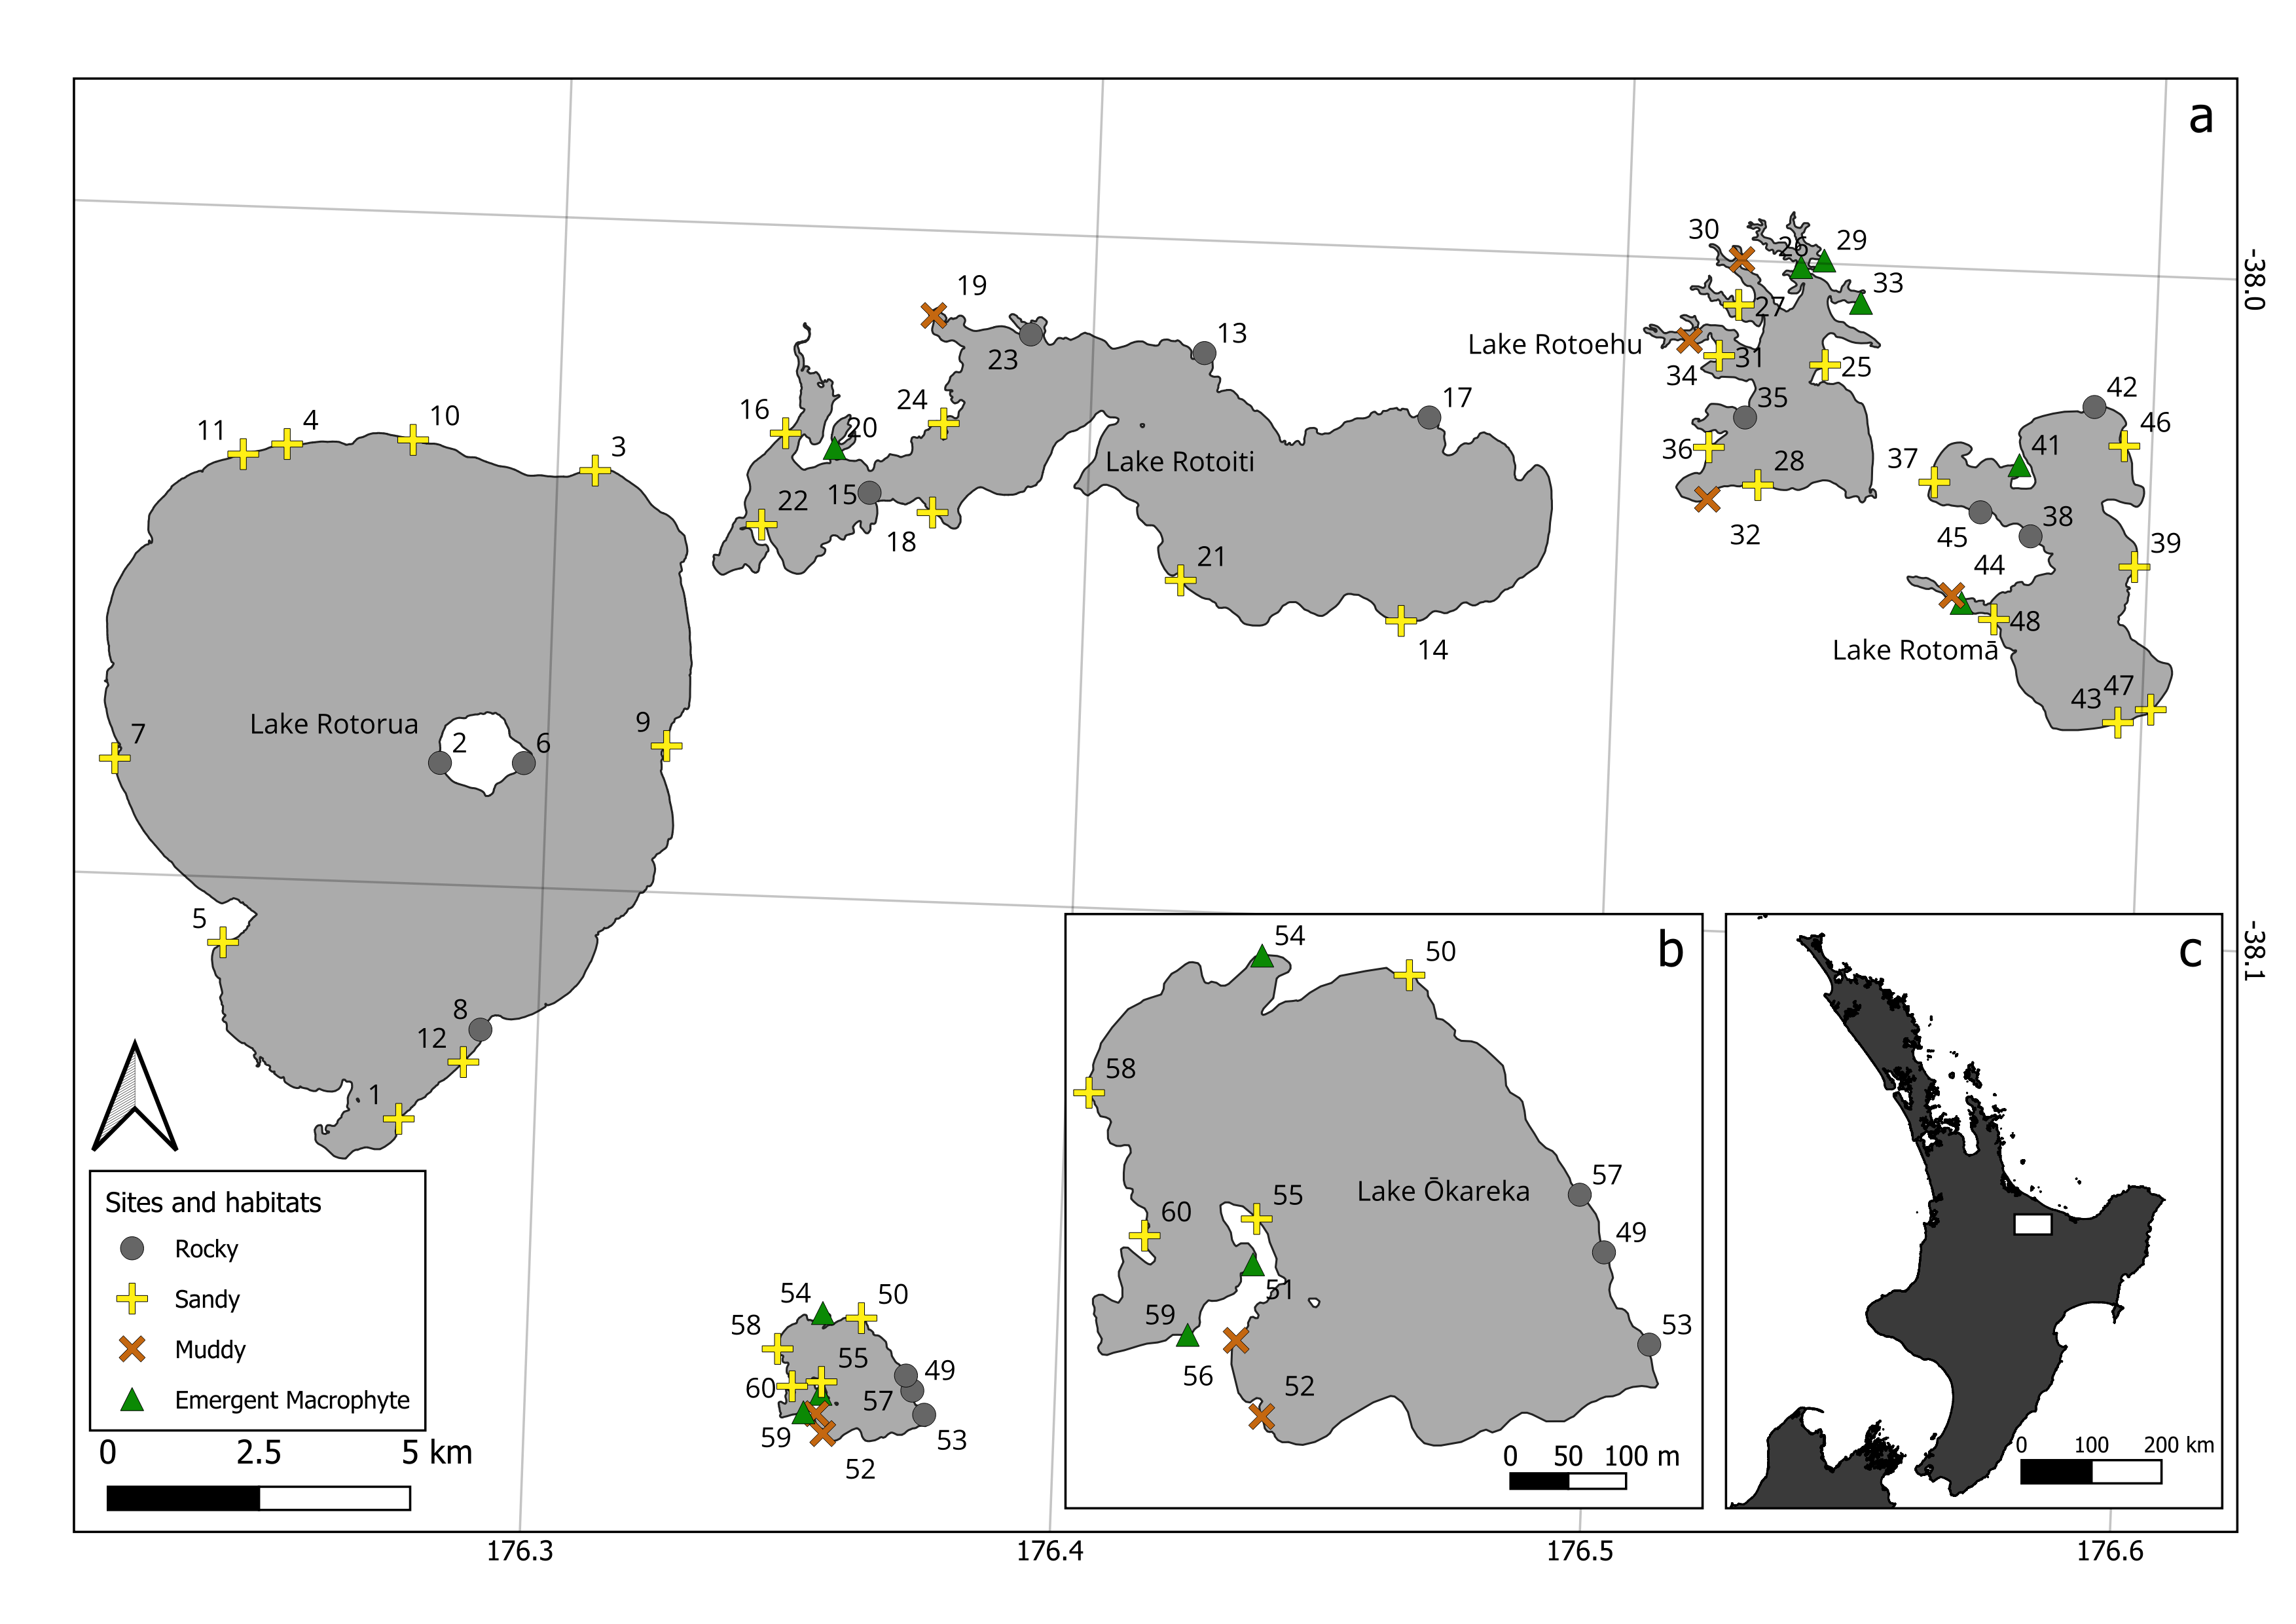
\includegraphics[width=0.8\linewidth,height=\textheight,keepaspectratio]{images/Natural_habitat_map.png}

}

\caption{\label{fig-site-map}Map of the sampling locations with
different dominant littoral habitat types classified. a) Overview map of
the 5 lakes. Lakes where invasive catfish were detected are indicated.
b) Zoom in of Lake Ōkāreka. c) Guidance map to show the lakes location
(white square) on the North Island of Aotearoa New Zealand.}

\end{figure}%

\subsection{Data collection}\label{data-collection}

In total, 60 sampling sites were sampled once in the Austral
spring/summer from October 2024 to February 2025. Each sampling site
measured 15 × 10 m and extended from the shoreline into the lake. At
locations with unstable lake margins or depths exceeding 1 m,
observations and measurements were conducted from a boat. At each site,
physical, chemical and biological parameters were recorded
(Table~\ref{tbl-environmental-biotic-overview}).

\begin{landscape}
\begingroup\fontsize{7}{9}\selectfont

\begin{longtable}[t]{>{\raggedright\arraybackslash}p{2.5cm}>{\raggedright\arraybackslash}p{3.5cm}>{\raggedright\arraybackslash}p{9.5cm}>{\raggedright\arraybackslash}p{5.0cm}}

\caption{\label{tbl-environmental-biotic-overview}Overview of
environmental and biotic variables measured at littoral sampling sites,
including variable descriptions, units, and hypothesised relevance for
kōura (\emph{Paranephrops planifrons}). Variables were selected a priori
based on known habitat requirements, physiological constraints, and
potential biotic interactions influencing kōura occurrence, abundance,
and biomass in lake littoral zones.}

\tabularnewline

\toprule
Variable & Description / Unit & Hypothesised importance for kōura & References\\
\midrule
\cellcolor{gray!8}{Lake identity} & \cellcolor{gray!8}{Categorical variable identifying lake} & \cellcolor{gray!8}{Captures unmeasured lake-specific differences in water chemistry, productivity, and catchment characteristics.} & \cellcolor{gray!8}{Zuur et al., (2009)}\\
Substrate index & Index based on \% cover of bedrock, boulders, cobble, gravel, sand, mud, and organic matter & Important for burrowing and shelter availability. Coarser substrates increase shelter availability through more crevices. & Usio \& Townsend, (2000); Kusabs et al., (2015b)\\
\cellcolor{gray!8}{Slope} & \cellcolor{gray!8}{Slope from shoreline to the 5 m depth contour} & \cellcolor{gray!8}{Steeper slopes facilitate access to deeper water during daylight refuging and associate with coarser substrates.} & \cellcolor{gray!8}{Devcich, (1979); Kusabs et al., (2015b)}\\
Riparian vegetation & Percentage cover of vegetation growing in the riparian zone & Contributes detrital inputs, bank stability, and shading at the water's edge. & Parkyn et al., (2002)\\
\cellcolor{gray!8}{Overhanging trees} & \cellcolor{gray!8}{Percentage cover of trees hanging over the shoreline} & \cellcolor{gray!8}{Provides direct shading and structural inputs into littoral habitats.} & \cellcolor{gray!8}{Smith et al., (1996); Vedia et al., (2017)}\\
\addlinespace
Wood cover & Cover of wooden logs and tree branches in the sample site & Provides physical structure creating refuge spaces and supports macroinvertebrate prey availability. & Parkyn et al., (2009)\\
\cellcolor{gray!8}{Emergent and submerged macrophytes} & \cellcolor{gray!8}{Percentage cover of macrophytes in the sample site divided over emergent and submerged and native and non-native species} & \cellcolor{gray!8}{Native macrophytes can provide cover and serve as a food source. Non-native macrophytes may alter movement pathways and modify local habitat and water quality conditions.} & \cellcolor{gray!8}{Coffey \& Clayton, (1988); Kusabs \& Quinn, (2009)}\\
Temperature & Temperature of surface water in °C & Influences metabolic rate, activity, physiological stress, and habitat suitability. & Devcich, (1979); Hammond et al., (2006); Parkyn \& Collier, (2002); Angilletta et al., (2004)\\
\cellcolor{gray!8}{Dissolved oxygen} & \cellcolor{gray!8}{Dissolved oxygen concentration in mg L⁻¹} & \cellcolor{gray!8}{Essential for respiration; reduced oxygen may constrain activity and habitat use.} & \cellcolor{gray!8}{Hammond et al., (2006); Broughton et al., (2017)}\\
Specific conductivity & Electrical conductivity of the water in µS cm⁻¹ & Reflects overall lake productivity, supporting food availability. & Devcich, (1979)\\
\addlinespace
\cellcolor{gray!8}{pH} & \cellcolor{gray!8}{Acidity or alkalinity of the water} & \cellcolor{gray!8}{Influences moulting success and exoskeleton strength, affected by acidity or calcium levels.} & \cellcolor{gray!8}{Olsson et al., (2006)}\\
Fish presence & Presence/absence of selected native and non-native fish species & Fish act as predators, competitors, or indirectly modify habitat structure. & Shave et al., (1994); Barnes, (1996); Usio \& Townsend, (2000); Barnes \& Hicks, (2003)\\
\bottomrule

\end{longtable}

\endgroup{}
\end{landscape}

Physical characteristics were assessed using both visual estimates and
field measurements. Substrate composition was visually estimated with an
underwater viewing chamber, as water clarity was sufficiently clear at
all sites, using a standardised classification scheme, categorising
bedrock, boulders (\textgreater256 mm), cobble (64--256 mm), gravel
(2--64 mm), sand (0.063--2 mm), mud (\textless0.063 mm), and organic
matter. A substrate index was then calculated from these estimates using
a formula adapted to include fine organic matter and mud (Jowett and
Richardson 1990; Jowett et al. 2008; Harding et al. 2009):

\[
\begin{aligned}
\text{Substrate index} &= 0.08 \times (\text{bedrock}) + 0.07 \times (\text{boulders}) \\
&\quad + 0.06 \times (\text{cobble}) + 0.04 \times (\text{gravel}) + 0.03 \times (\text{sand}) \\
&\quad + 0.02 \times (\text{organic matter}) + 0.01 \times (\text{mud})
\end{aligned}
\]

Larger substrate classes were assigned higher weights because coarse
substrates such as cobble and boulders create greater interstitial pore
spaces and stable structures that kōura use as refuge from predators.
Coarse substrate availability has been shown to mediate crayfish
vulnerability to predation and directly influence crayfish abundance in
lakes (Usio and Townsend 2000; Nyström et al. 2006), whereas fine
substrates such as silt and mud alone offer limited physical refugia.
Fine substrates were assigned near-zero coefficients (0.01--0.03),
making their contribution to the index minimal relative to coarse
substrates (0.06--0.08), consistent with the positive-weighting
structure of the original index (Jowett and Richardson 1990). Riparian
vegetation, overhanging tree cover, and wood debris was visually
estimated as percentage cover within each site, along with emergent,
submerged, and turf vegetation cover. To assess proximity to deeper
waters, slope was calculated as horizontal distance from the shoreline
to the 5 m depth contour derived from bathymetric maps. Chemical
parameters included water temperature (°C), dissolved oxygen (mg
L\(^{-1}\)), and conductivity (\(\mu\)S cm\(^{-1}\)), measured with a
YSI ProSolo meter (Pro2030 Dissolved Oxygen and Conductivity Meter, YSI
Inc., Yellow Springs, OH, USA) and pH was determined using a handheld pH
meter (EC-PCTestr35, Eutech Instruments Pte Ltd, Paisley, UK).

Catch data for kōura and fish were collected using two single-winged,
double-throated fyke nets (600 mm high D-shaped entrance hoop) and two
collapsible bait traps baited with trout flesh (480 × 250 mm; two 50 mm
entrance openings). Fyke nets were placed perpendicular to the shoreline
at 10 m intervals, with bait traps positioned between them. All
equipment was deployed simultaneously at each site for a 24-h period.
The use of two fyke nets and two baited bait traps per site was intended
to maximise detection probability across habitat types. Captured kōura
were measured for orbital carapace length (OCL) using a digital calliper
(0.01 mm precision; 150 mm) and for wet mass using a digital scale (±1
g; 5 kg capacity, Anko Brand, Kmart Group, Mulgrave, VIC, Australia).
Catfish and other fish species, including eels (\emph{Anguilla} spp.),
goldfish (\emph{Carassius auratus} (Linnaeus, 1758)), common smelt
(\emph{Retropinna retropinna} (Richardson, 1848)), kōaro (\emph{Galaxias
brevipinnis} Günther, 1866), rainbow trout, common bully
(\emph{Gobiomorphus cotidianus} McDowall \& Fulton, 1978), and
mosquitofish (\emph{Gambusia affinis} (S. F. Baird \& Girard, 1853)),
were recorded for abundance and measured for total length, and weighed
for wet mass. Catch per unit effort (CPUE) and biomass per unit effort
(BPUE) were calculated for all kōura and fish based on the number of
nets and traps used at each site (Kusabs et al. 2015b). Missing kōura
weights due to failure of scale (n = 81) were estimated using a
log₁₀--log₁₀ length--weight regression fitted to individuals with both
measurements (n = 240), following standard approaches for weight length
relationships in aquatic organisms
({Figure~\ref{fig-length-weight-ch3}}) (Froese 2006). Predicted values
were back-transformed with a lognormal bias correction factor
\(10^{0.5 \sigma^2}\) (Quinn and Keough 2002).

\[
\log_{10}(\text{Weight [g]}) = -2.938 + 2.864 \times \log_{10}(\text{OCL length [mm]})
\]

\subsection{Data analyses}\label{data-analyses}

Because each site was sampled only once, imperfect detection could not
be estimated separately from occupancy. Presence--absence data therefore
reflect observed detections at the time of sampling, and sites where
kōura were not captured were treated as absences in the models. As a
result, inference focuses on relative associations between kōura
occurrence and environmental or biotic predictors, rather than on
estimating true occupancy probabilities.

Kōura presence or absence, CPUE, and BPUE were analysed using
mixed-effects models to account for non-independence among sampling
sites (Bolker et al. 2009). To test for differences among lakes, kōura
presence was modelled using a binomial generalised linear mixed model
(GLMM; logit link). CPUE and BPUE were modelled using Tweedie GLMM (log
link), which is appropriate for continuous non-negative data with high
frequency of zeros, as common in ecological count and biomass data
(Shono 2008). These models were fitted using the glmmTMB package (Brooks
et al. 2017), with habitat type included as a random intercept. To
identify environmental and biotic predictors associated with kōura
distribution and abundance, GAMMs were implemented with the mgcv package
(Wood 2004, 2017). To reduce multicollinearity, predictors were screened
using Variance Inflation Factors (VIFs) calculated from linear models
fitted to the fixed-effect design matrix. A conservative threshold of
VIF \textgreater{} 5 was applied (Quinn and Keough 2002; Kutner et al.
2005). Across all model sets, dissolved oxygen expressed as percentage
saturation (DO \%) exceeded this threshold and was excluded from further
analyses, while dissolved oxygen concentration (DO mg L\(^{-1}\)) was
retained.

For occupancy analyses, kōura presence--absence was modelled using a
binomial GAMM with a logit link function (Zuur et al. 2009; Wood 2017).
For CPUE and BPUE, a hurdle modelling approach was adopted due to the
high frequency of zero observations in the data. In this approach,
occurrence (zero vs non-zero values) was modelled using a binomial GAMM
with a logit link, followed by modelling of positive CPUE or BPUE values
using Gamma GAMMs with a log link. This framework allows occurrence and
positive abundance to be modelled separately and is appropriate for
datasets characterised by many zero observations. Hurdle models are
commonly used with freshwater crayfish catch data, which often possess
these features (Rosewarne et al. 2013). Environmental and biotic
predictors considered included substrate index, slope to 5 m depth,
riparian vegetation, overhanging trees, wood cover, aquatic vegetation
classes (emergent native, submerged native, submerged non-native, and
emergent non-native vegetation), water temperature (°C), dissolved
oxygen (mg L\(^{-1}\)), pH, specific conductivity (\(\mu\)S
cm\(^{-1}\)), and the presence of catfish, eels, goldfish, and common
smelt. Continuous predictors were centred and standardised prior to
modelling to improve convergence and facilitate comparison of effect
sizes and were modelled as smooth terms using thin plate regression
splines (bs = `ts'), which apply additional shrinkage to penalise overly
complex relationships and can shrink smooth terms fully to zero during
selection (Wood 2017). Basis dimensions (k) were set based on the number
of unique values per predictor and adjusted where necessary to balance
flexibility and parsimony. Binary predictors (fish presence variables)
were included as parametric terms.

Model selection was performed using maximum likelihood estimation with
stepwise backward elimination, sequentially removed and the model
refitted until all remaining terms met the retention threshold
(\(\alpha\) ≤ 0.05). Reduced models were compared with their respective
full models using likelihood ratio tests and Akaike Information
Criterion (AIC) scores. Final selected models were refitted using
restricted maximum likelihood (REML), which accounts for the degrees of
freedom associated with fixed effects and provides less biased estimates
of variance components, resulting in more stable smoothing parameter
estimates in models with random effects. Lake identity was included as a
random effect in all GAMMs to account for spatial clustering and
non-independence among observations and was not subject to the variable
selection procedure (Zuur et al. 2009).

Model diagnostics were performed to evaluate model fit and assumptions.
Residuals were inspected to assess homogeneity of variance and normality
(Zuur et al. 2009). Concurvity, the degree to which smooth terms can be
approximated by other smooths in the model, was assessed to identify
potential instability in smooth term estimates (Wood 2017). Basis
dimension checks using effective degrees of freedom (edf) were performed
to ensure smoothing terms had sufficient flexibility to capture
underlying patterns without overfitting (Zuur et al. 2009). For binomial
components, model discrimination was evaluated using Receiver Operating
Characteristic and Area Under the Curve (ROC/AUC), where values
approaching 1 indicate perfect discrimination between presences and
absences (Fielding and Bell 1997). For positive-only abundance models,
predicted versus observed values were compared to assess how well the
model reproduces observed CPUE and BPUE values across the range of the
data.

To provide context for the association between catfish presence and
kōura metrics detected in the GAMM, a descriptive comparison of kōura
presence rate, CPUE, and BPUE was conducted across catfish-present and
catfish-absent sites, and across lakes with and without catfish.

\section{Results}\label{results-1}

A total of 321 kōura were captured across 33 of the 60 surveyed sites
within the five Rotorua Te Arawa Lakes. Kōura OCL ranged from 7--53 mm
and individual body mass from 0.2--87 g. Kōura were detected in all five
lakes; however, abundance varied among lakes, with total counts ranging
from 19 to 112 individuals. Mixed-effects models indicated a significant
effect of lake on kōura occupancy (binomial GLMM: likelihood ratio test,
\(\chi^2_{4} = 13.76\), \emph{p} = 0.008), CPUE (Tweedie GLMM:
\(\chi^2_{4} = 12.60\), \emph{p} = 0.013), and BPUE (Tweedie GLMM:
\(\chi^2_{4} = 9.66\), \emph{p} = 0.047;
Figure~\ref{fig-koura-by-lake}).

\begin{figure}

\centering{

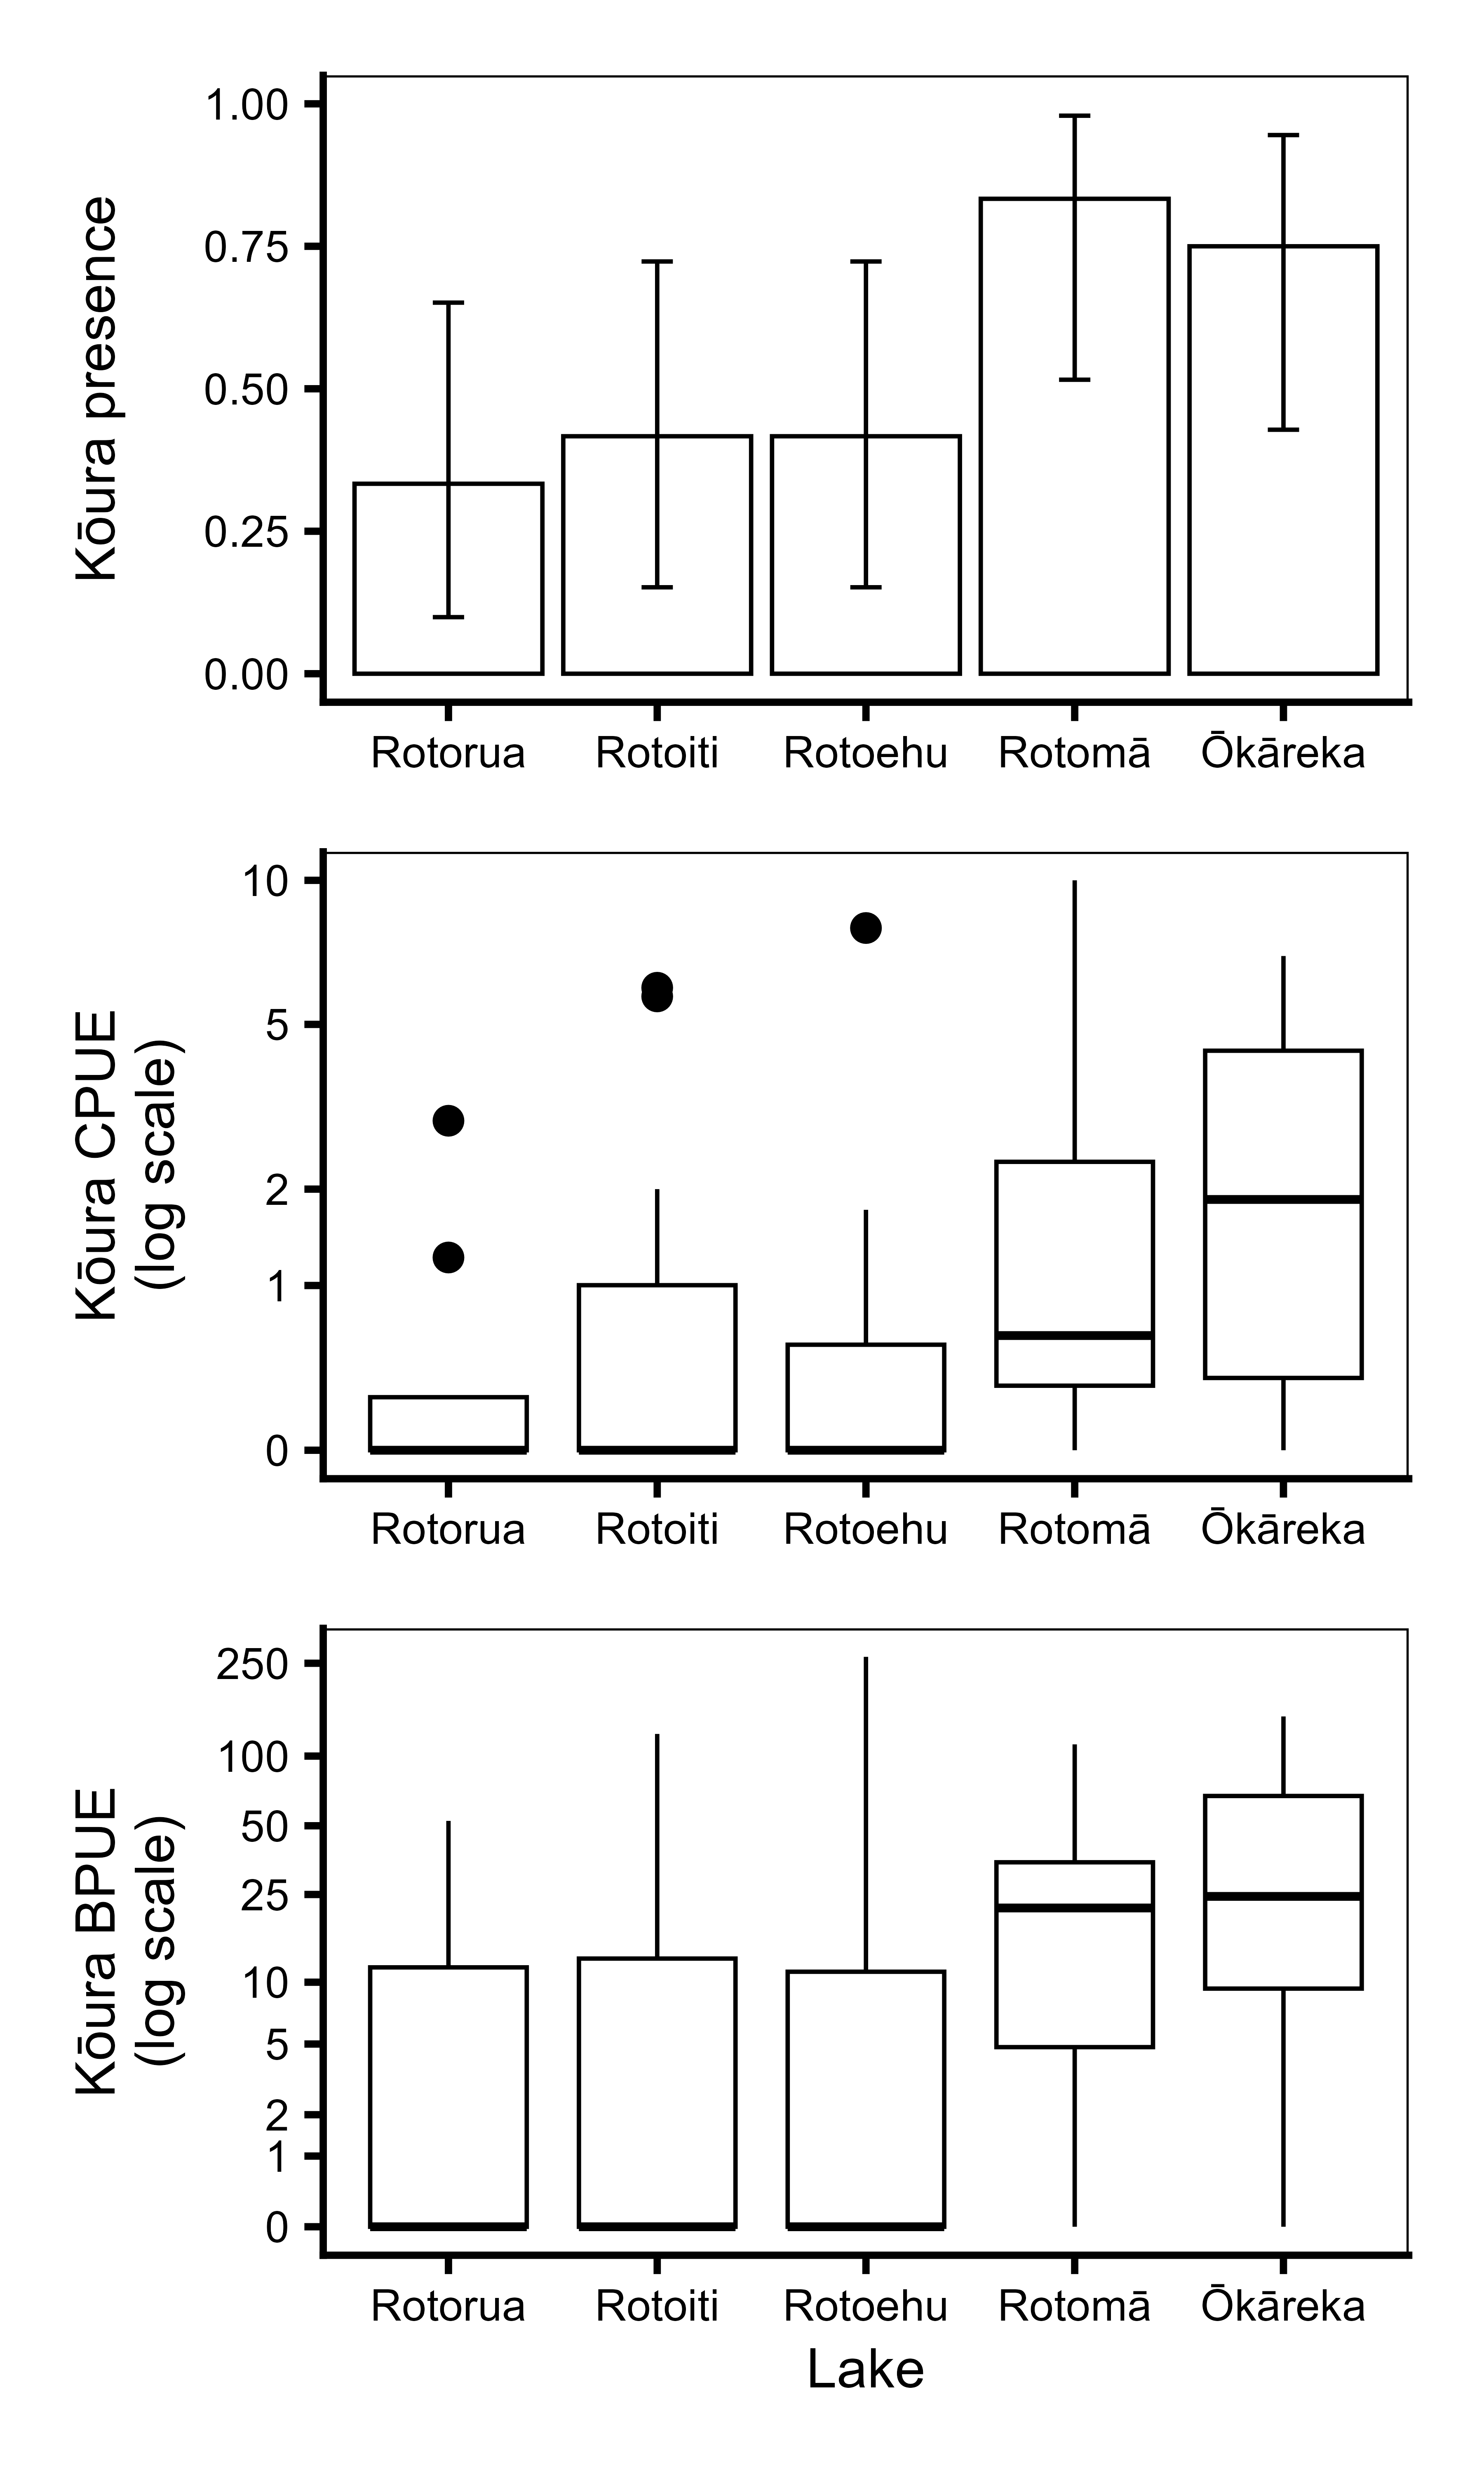
\includegraphics[width=0.5\linewidth,height=\textheight,keepaspectratio]{outputs/fig-koura-by-lake.png}

}

\caption{\label{fig-koura-by-lake}Kōura presence, CPUE, and BPUE across
lakes. The upper panel shows the proportion of sampled sites with kōura
present in each lake, with error bars indicating 95\% binomial
confidence intervals. The middle and lower panels show the distribution
of kōura CPUE and BPUE, respectively, across lakes using boxplots
(median, interquartile range, and range).}

\end{figure}%

The five lakes differed substantially in environmental and biotic
characteristics ({Table~\ref{tbl-an-env-fish-summary}}). Physical
habitat structure varied among lakes, with differences in substrate
index, nearshore slope, and littoral vegetation cover. Emergent
macrophytes were absent from Lake Rotorua but present in the other
lakes, particularly Ōkāreka, while submerged macrophyte cover at the
shore was rare in Rotorua and Rotoiti but more extensive in Rotoehu and
Rotomā. Water chemistry also differed markedly among lakes. Surface
water temperatures were highest in Rotorua and lowest in Rotomā and
Ōkāreka, while pH ranged from circum-neutral conditions in Rotorua to
more alkaline conditions in Rotoehu and Rotoiti. Specific conductivity
showed strong contrasts, being highest in Rotoehu and lowest in Ōkāreka.
Dissolved oxygen concentrations in the littoral zone varied less among
lakes but were generally lowest in Rotorua. Fish populations differed
between lakes, reflecting invasion history. Catfish were detected only
in Lakes Rotorua and Rotoiti, whereas goldfish occurred in all lakes but
were most abundant in Rotoehu. Common bullies were found in every survey
location. Trout were found sporadically in Rotorua, Rotoiti and Ōkāreka
and kōaro were only caught from Ōkāreka.

\subsection{Kōura occupancy}\label{kux14dura-occupancy}

The full binomial GAMM for kōura occupancy explained 65 \% of the
deviance (AIC = 51; adj. R² = 0.647). Stepwise ML reduction
(\(\alpha = 0.05\)) retained riparian vegetation, substrate index,
temperature, and specific conductivity as smoother terms, lake identity
as a random effect, and the presence of goldfish (negative) and catfish
(positive) as parametric terms. The final model refitted using REML
explained 57.9 \% of the deviance (adj. R² = 0.592) and retained
positive influences of riparian vegetation (\emph{p} = 0.026), substrate
index (\emph{p} = 0.001), specific conductivity (\emph{p} = 0.002) and a
negative influence of temperature (\emph{p} \textless{} 0.001), as
significant smoother terms (Figure~\ref{fig-occupancy-model} a). The
random effect of lake identity was not statistically significant
(\emph{p} = 0.622), indicating limited residual variation between lakes
after accounting for environmental and biotic predictors. Among the
parametric covariates, goldfish had a significant negative relationship
(\emph{p} = 0.017), and catfish presence showed a significant positive
relationship (\emph{p} = 0.014). Model diagnostics showed no evidence of
overfitting (edf \textless{} k) and good discrimination (AUC = 0.946;
Figure~\ref{fig-occupancy-model} b). Concurvity diagnostics revealed
high collinearity between specific conductivity and lake identity
(worst-case = 1.00, observed = 0.94), and between temperature and lake
identity (worst-case = 0.95, observed = 0.88), suggesting both
predictors partly reflect between-lake differences. Residual diagnostics
showed no systematic patterns in variance across fitted values,
consistent with acceptable model fit for a binomial GAMM. The
calibration plot indicated slight under-prediction at low probabilities
and slight over-prediction at mid-range probabilities
(Figure~\ref{fig-occupancy-model} c). The binomial components of the
CPUE and BPUE hurdle models produced the same structure and effect
directions as the occupancy model, so only the positive Gamma components
are reported here.

\begin{figure}

\centering{

\includegraphics[width=0.8\linewidth,height=\textheight,keepaspectratio]{outputs/fig-occupancy-model.png}

}

\caption{\label{fig-occupancy-model}Kōura occupancy GAMM results and
model performance. a) Estimated smooth terms for riparian vegetation,
substrate index, surface water temperature, and specific conductivity,
shown as partial effects with 95\% confidence intervals. See Fig. S2 for
raw data underlying modelled relationships. b) Receiver operating
characteristic (ROC) curve illustrating model discrimination, with the
area under the curve (AUC) reported. c) Calibration plot based on five
equal-frequency bins, comparing mean predicted occupancy probabilities
with observed proportions of occupied sites; the dashed 1:1 line
indicates perfect calibration.}

\end{figure}%

\subsection{Kōura CPUE}\label{kux14dura-cpue}

The full Gamma GAMM for positive CPUE explained 48.4 \% of the deviance
(AIC = 122; adj. R² = 0.19; n = 33). Stepwise selection
(\(\alpha = 0.05\)) reduced the model to temperature, pH, and emergent
native macrophytes as smoother terms, lake identity as a random effect,
and the presence of common smelt (negative) as a parametric effect. This
reduced model achieved a lower AIC (115) and explained 47.3 \% of the
deviance (adj. R² = 0.194). Likelihood ratio tests indicated that the
reduced model was statistically equivalent to the full model (\emph{p} =
0.950), and it was therefore selected as the final CPUE model.

The final REML-fitted model explained 47.3 \% of the deviance (adj. R² =
0.195) and retained positive influence of pH (\emph{p} \textless{}
0.001) and negative influence of temperature (\emph{p} = 0.019) and
emergent native macrophytes (\emph{p} \textless{} 0.001) as significant
smooth predictors (Figure~\ref{fig-cpue-hurdle} a). The lake identity
random effect was not significant (\emph{p} = 0.482), indicating minimal
additional between lake variation once environmental covariates were
included. Presence of common smelt had a significant negative parametric
relationship (\emph{p} = 0.041). Concurvity diagnostics indicated strong
correlation between temperature and pH, but both variables were retained
because they were ecologically interpretable and contributed
significantly to model fit. Model diagnostics showed no evidence of
overfitting (edf \textless{} k), and predictive accuracy was moderate
(Figure~\ref{fig-cpue-hurdle} b). Residual diagnostics showed no
systematic patterns in residual variance across fitted values. The model
tended to slightly over-predict very low CPUE values and under predict
the highest observations.

\begin{figure}

\centering{

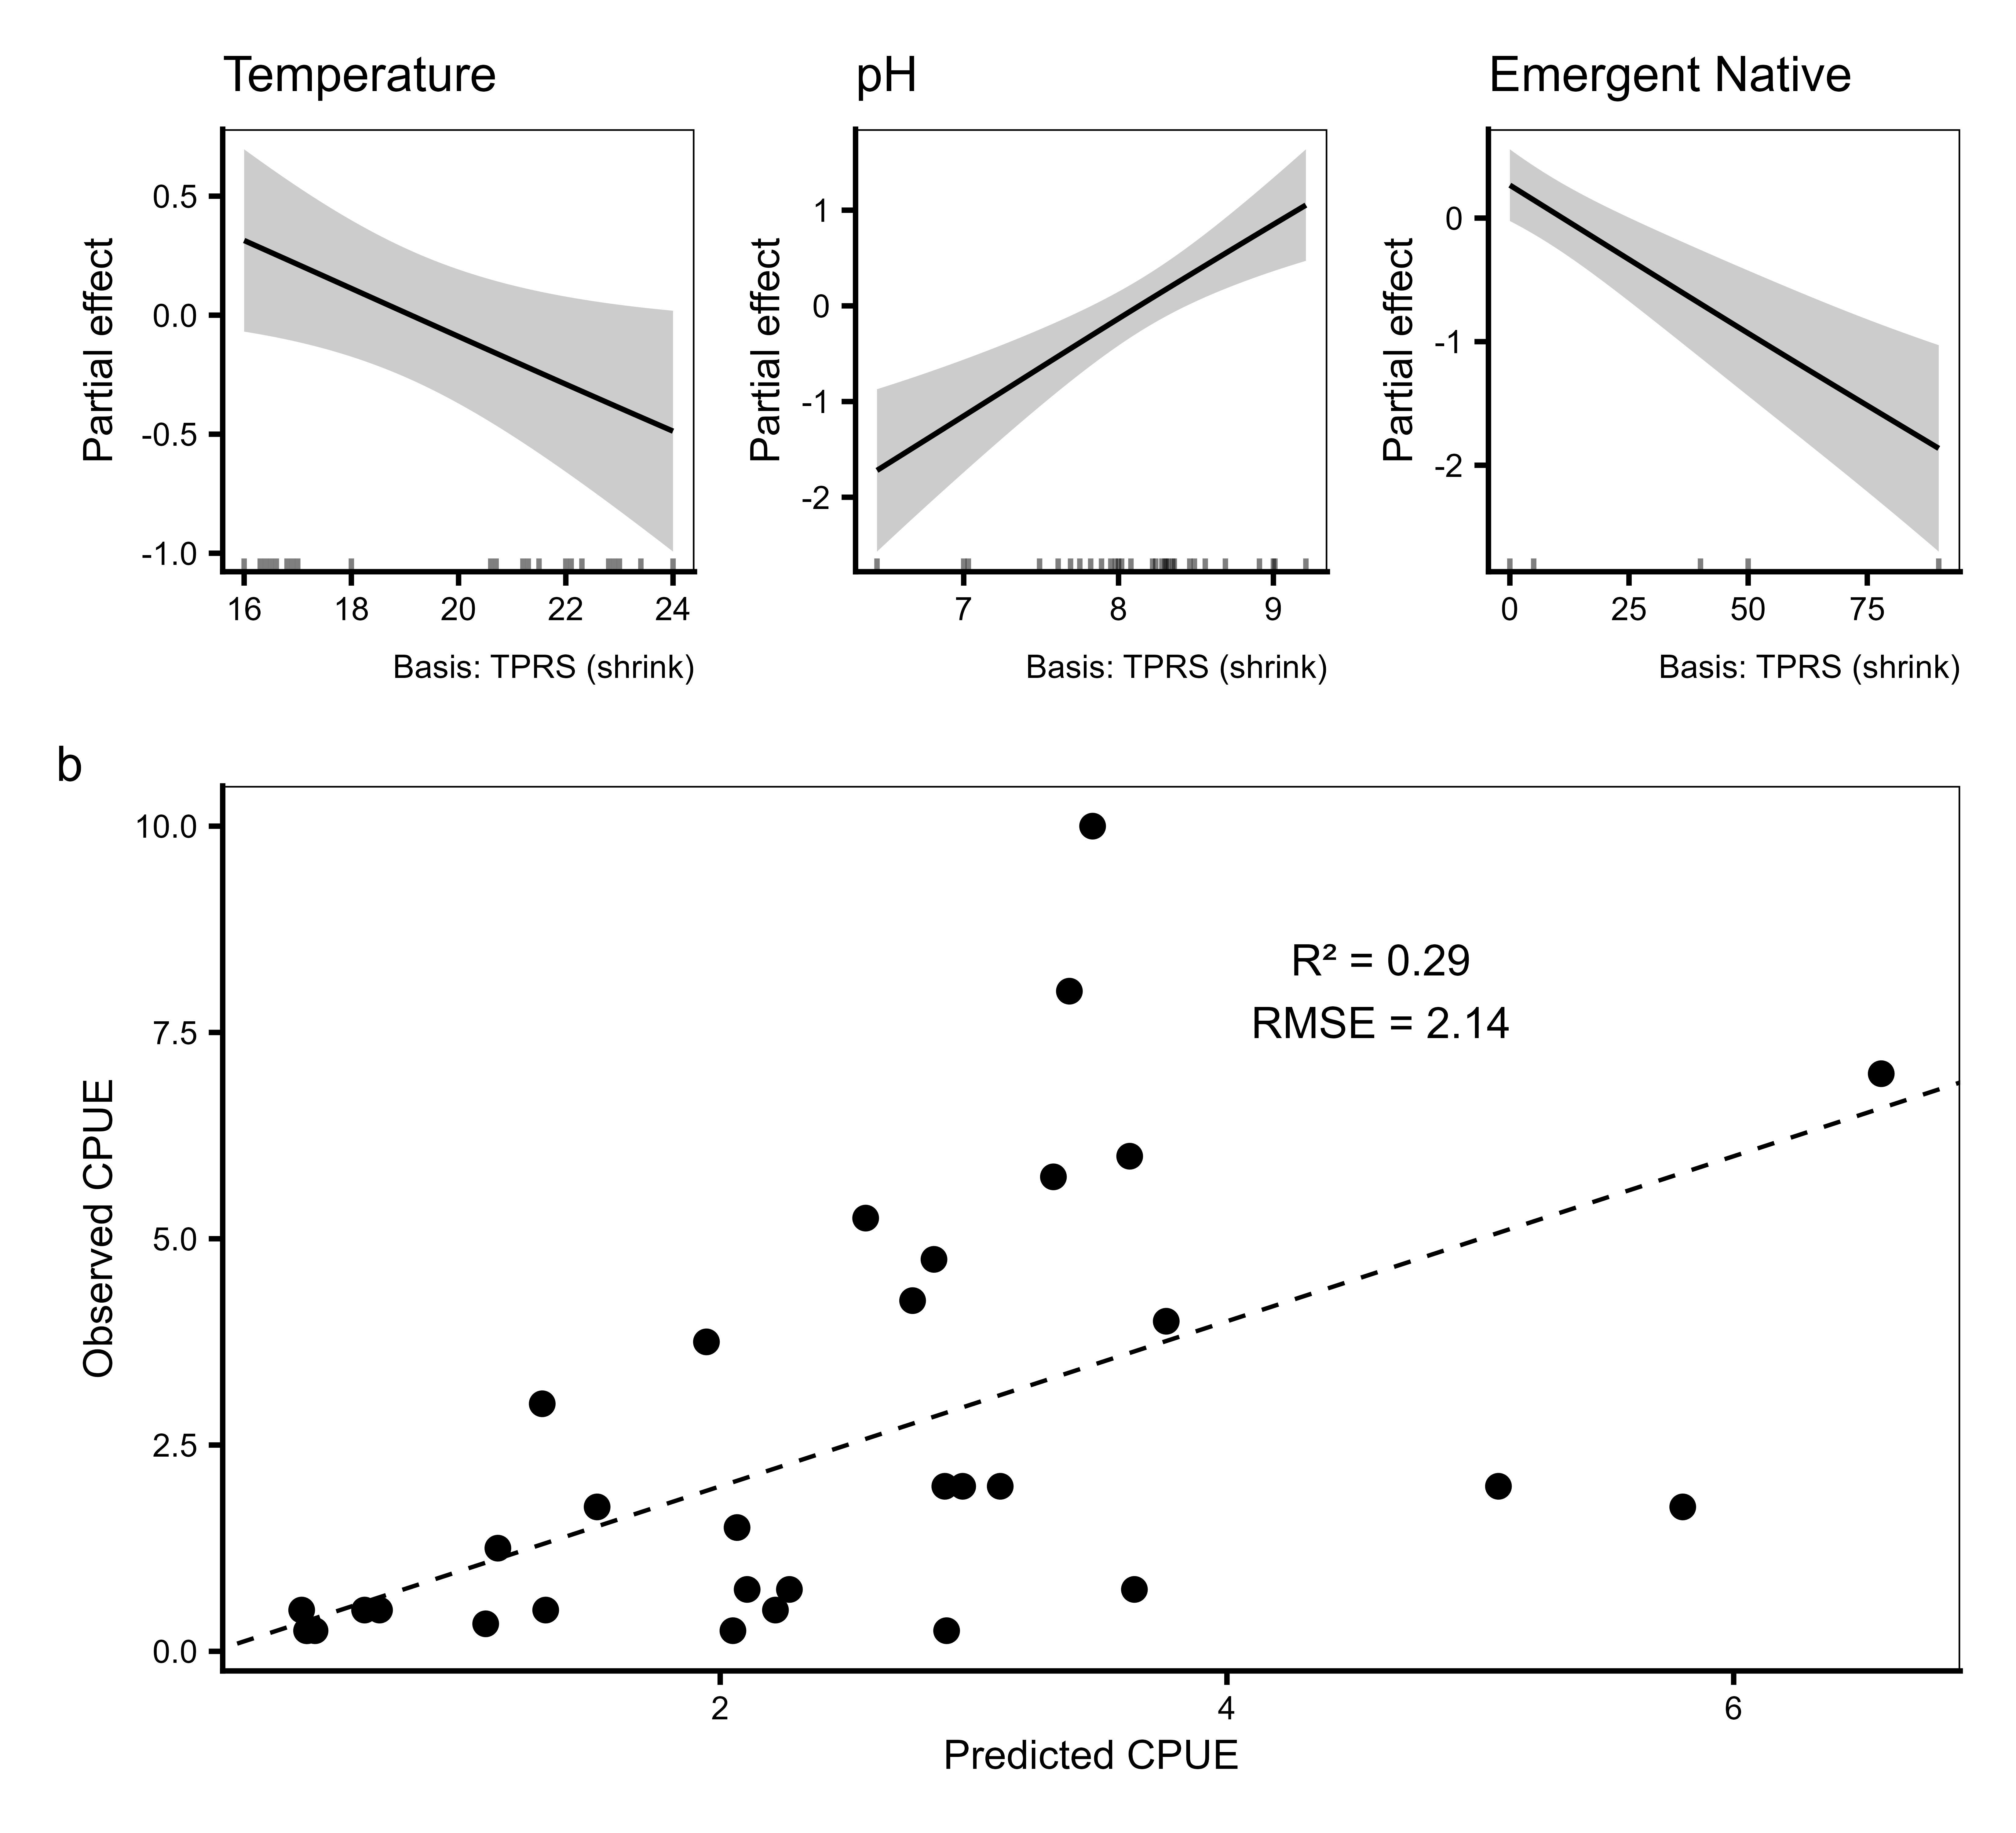
\includegraphics[width=0.8\linewidth,height=\textheight,keepaspectratio]{outputs/fig-cpue-hurdle.png}

}

\caption{\label{fig-cpue-hurdle}Kōura CPUE GAMM results and model
performance. a) Estimated smooth terms for surface water temperature,
pH, and emergent native macrophytes, shown with partial effects and 95\%
confidence intervals. See Fig. S2 for raw data underlying modelled
relationships. b) Predicted versus observed CPUE from the positive
(Gamma) component of the hurdle model, with predictions excluding the
random lake effect. The dashed 1:1 line indicates perfect agreement;
annotated values report R² and RMSE to summarise model fit.}

\end{figure}%

\subsection{Kōura BPUE}\label{kux14dura-bpue}

The full Gamma GAMM for positive BPUE explained 97.4 \% of the deviance
(AIC = 266; adj. R² = 0.76; n = 33). Stepwise ML selection
(\(\alpha = 0.05\)) retained pH, emergent native macrophytes, and the
lake identity random effect. The resulting reduced model had a higher
AIC (318) and explained 26 \% of the deviance (adj. R² = 0.141). As the
full model was overfitting the data the reduced model was chosen for
inference. The final REML-fitted BPUE model explained 25.9 \% of the
deviance (adj. R² = 0.14) and retained a positive influence of pH
(\emph{p} = 0.002) and a negative influence of emergent native
macrophytes (\emph{p} = 0.041) as significant, near-linear smoothing
(Figure~\ref{fig-bpue-hurdle} a). The emergent macrophyte effect, while
statistically significant, was close to the threshold and should be
interpreted with caution given the distributional limitations of the
model. The lake identity random effect was not significant (\emph{p} =
0.607), indicating minimal additional between lake variation after
accounting for environmental predictors. Diagnostic checks showed
appropriate basis dimensions (edf \textless{} k), stable convergence,
and acceptable levels of observed concurvity, though minor departure
from distributional assumptions was noted at the lower tail, likely
reflecting a small number of high-biomass sites. Predictive accuracy was
moderate (Figure~\ref{fig-bpue-hurdle} b), with a tendency for the model
to under predict the highest BPUE values.

\begin{figure}

\centering{

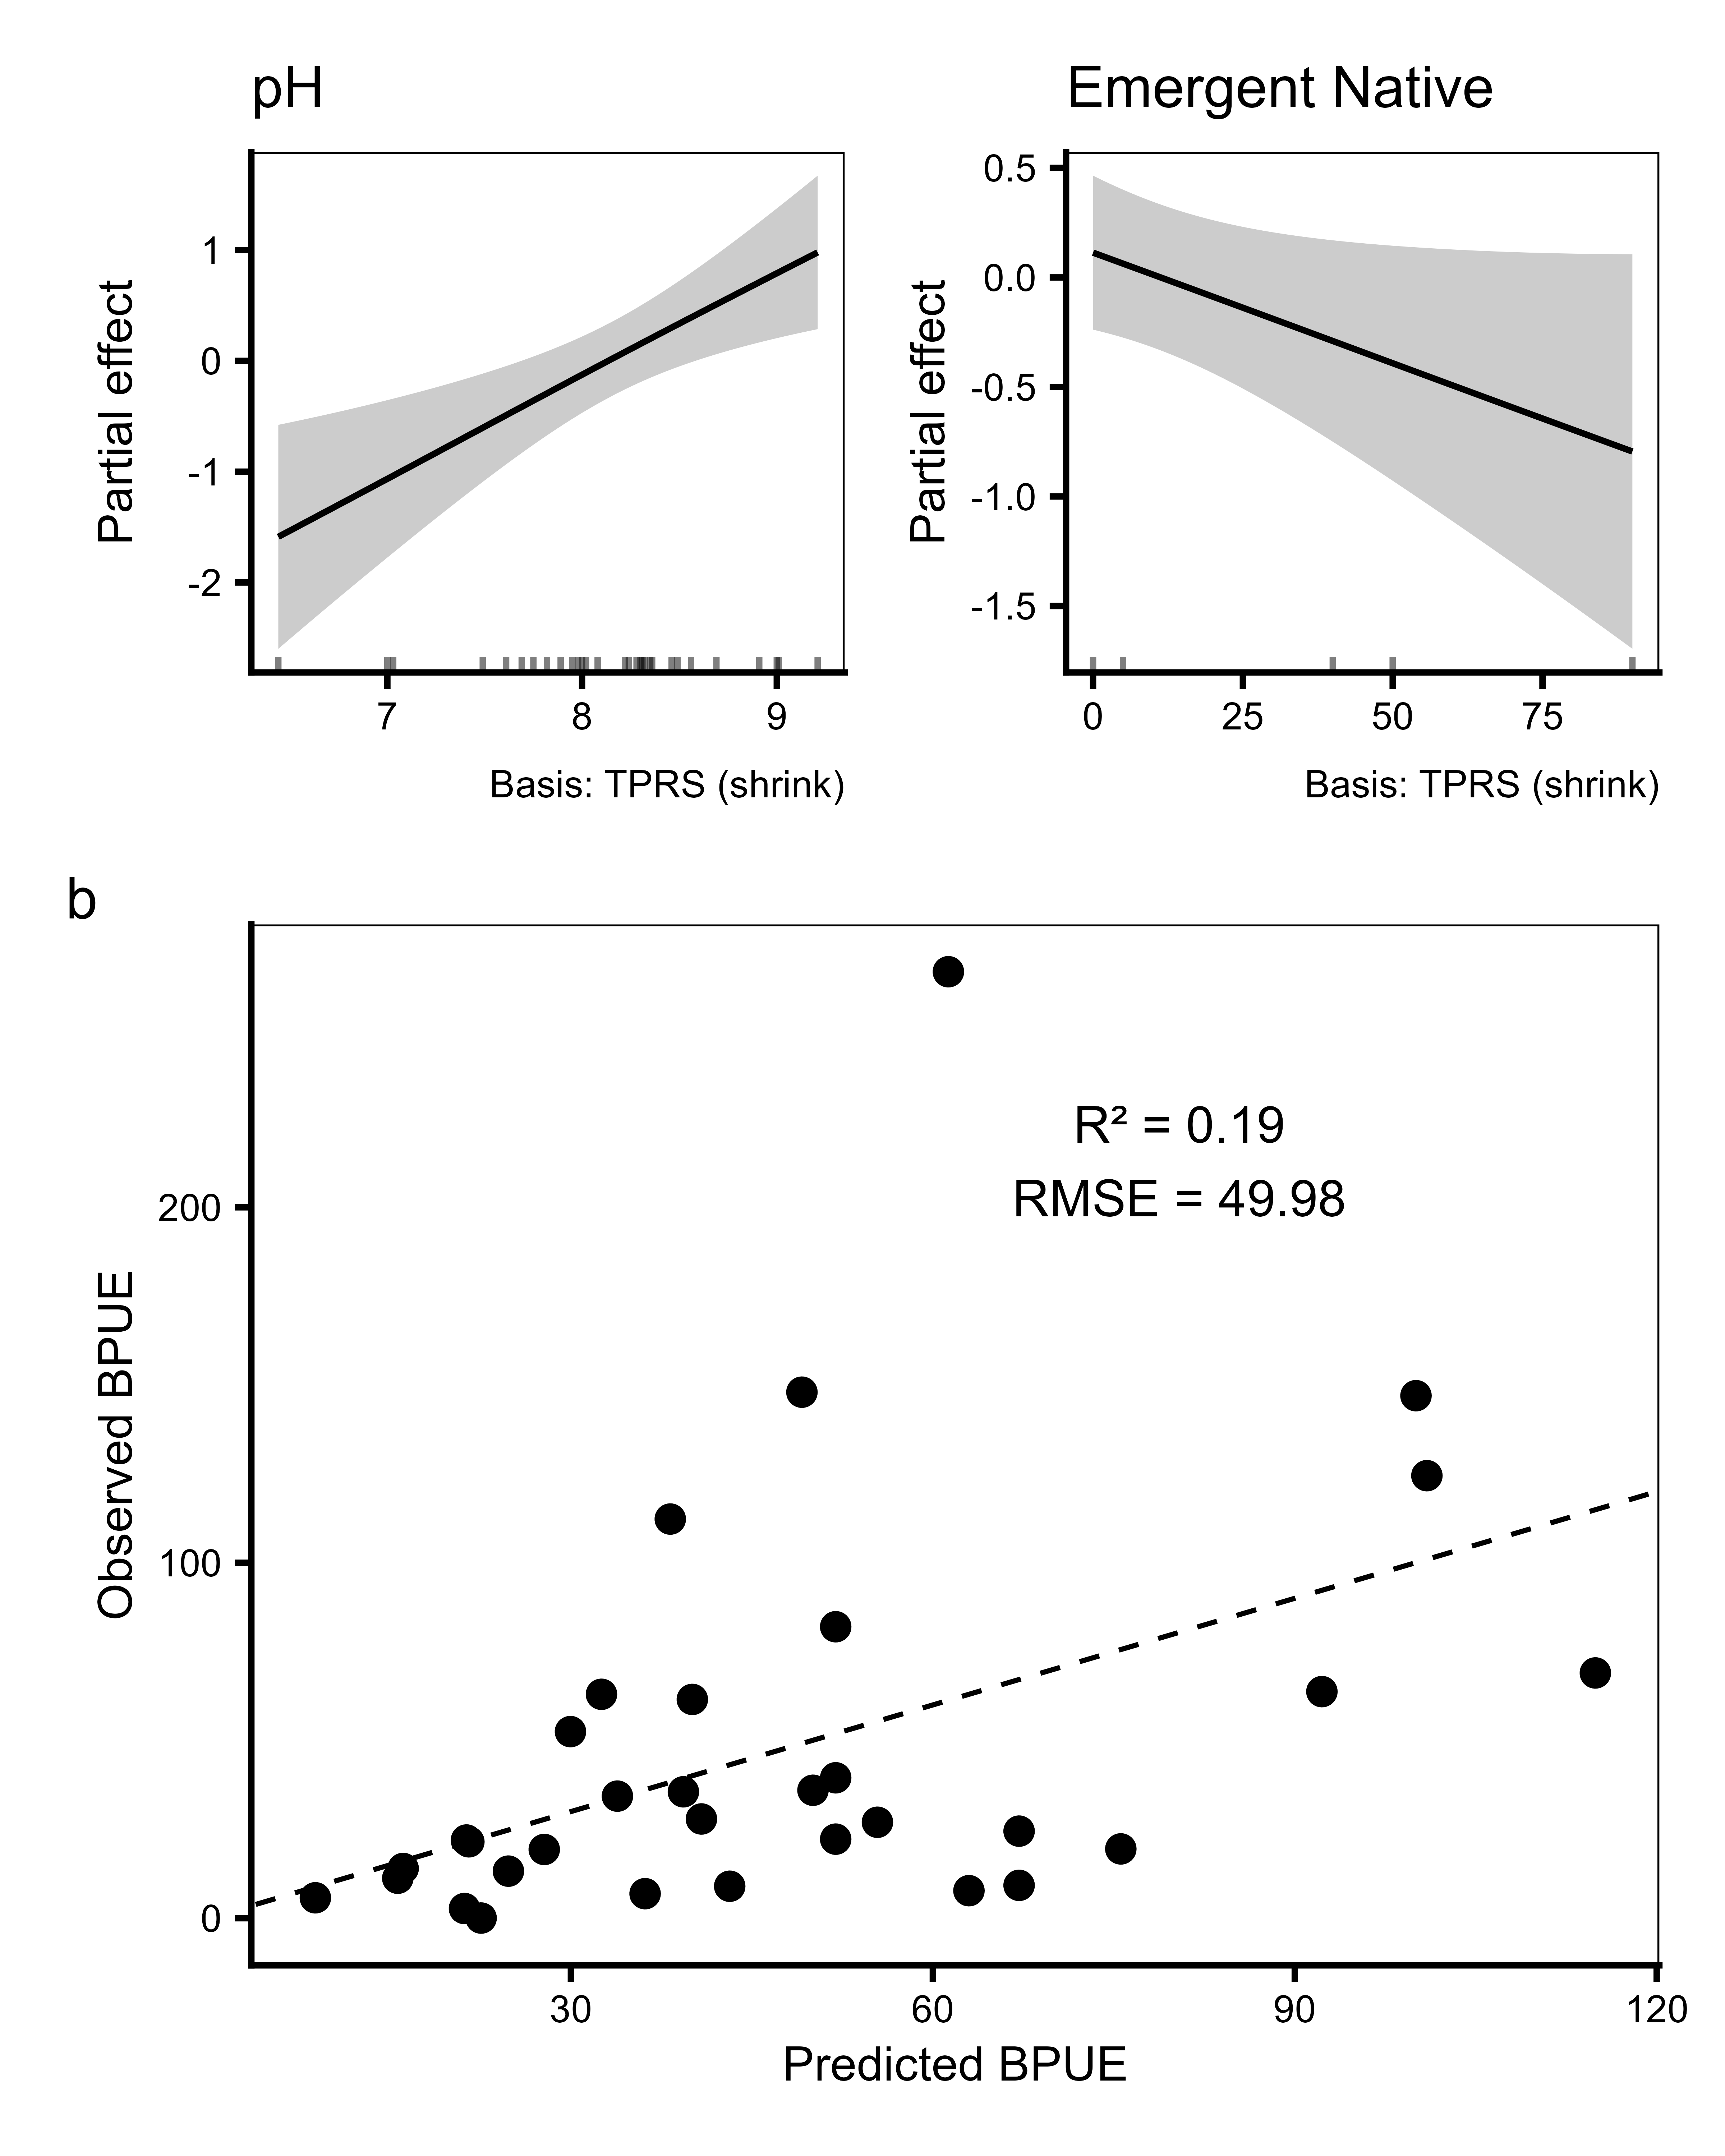
\includegraphics[width=0.65\linewidth,height=\textheight,keepaspectratio]{outputs/fig-bpue-hurdle.png}

}

\caption{\label{fig-bpue-hurdle}Kōura BPUE GAMM results and model
performance. a) Estimated smooth terms for pH and emergent native
macrophytes, shown with partial effects and 95\% confidence intervals.
See Fig. S2 for raw data underlying modelled relationships. b) Predicted
versus observed BPUE from the positive (Gamma) component of the hurdle
model, with predictions excluding the random lake effect. The dashed 1:1
line indicates perfect agreement; annotated values report R² and RMSE to
summarise model fit.}

\end{figure}%

\section{Discussion}\label{discussion-1}

We found that local and site-scale habitat characteristics were
consistently associated with kōura occurrence and abundance across the
five surveyed lakes. Although initial mixed-effects models identified
significant differences in kōura occupancy, Catch Per Unit Effort
(CPUE), and Biomass Per Unit Effort (BPUE) among lakes, these
differences were no longer evident once local environmental and biotic
predictors were incorporated into the Generalised Additive Mixed-Models
(GAMMs). However, interpreting the non-significance of lake identity in
the final models requires caution. In the occupancy model, both
temperature and specific conductivity showed near-perfect collinearity
with lake identity, suggesting these predictors likely absorbed
between-lake differences rather than capturing purely within-lake
habitat associations. Given that predictors were often correlated at the
site scale, the GAMMs are best interpreted as identifying habitat
associations rather than mechanistic drivers of kōura distribution. The
predictors substrate index and riparian vegetation cover, which varied
considerably within lakes, likely reflect genuine within-lake habitat
associations. Consequently, targeted management actions that improve
local habitat structure and address key biotic pressures at finer
spatial scales have the potential to deliver local gains, particularly
where whole-lake interventions are not feasible or where local habitat
degradation is the dominant stressor.

\subsection{Habitat associations with
kōura}\label{habitat-associations-with-kux14dura}

Kōura occurrence was consistently associated with coarser substrate
types and greater riparian vegetation cover. Substrate heterogeneity was
moderately negatively correlated with the substrate index (r = −0.48),
indicating that the index reflects dominance of coarse substrates rather
than proportional mixing of particle sizes. Higher substrate index
values therefore reflect the presence of large particles like bedrock,
boulders and cobbles, which create large interstitial pore spaces that
function as physical refugia, providing shelter from predators (White
and Irvine 2003; Haschenburger and Roest 2009; Kusabs et al. 2015b). The
relationship between substrate size and benthic invertebrates is not
linear (Quinn and Hickey 1990), where larger pore spaces between coarse
particles may favour adult kōura, smaller interstitial spaces within
mixed substrates may provide refugia for juveniles, suggesting that
heterogenous substrates support kōura across life stages. However, mixed
substrates containing both coarse and fine particles can reduce pore
space availability as smaller particles infill void spaces between
larger ones (Haschenburger and Roest 2009), meaning that dominance of
coarse substrate rather than substrate heterogeneity is the more
relevant driver of refugia availability for adults. Additionally coarse
substrates may facilitate burrowing by kōura at the margins of rocky
areas where softer sediments are accessible, providing an additional
form of refuge (Usio and Townsend 2000). Similar preferences for coarse
substrates have been reported in stream environments (Olsson et al.
2006; Jowett et al. 2008), although the optimal substrate size may
differ between habitat types. In streams, kōura show a non-linear
response to substrate size with an optimum around 130 mm, with
probability of occurrence declining at boulder substrates larger than
256 mm, likely because larger substrates are associated with higher flow
velocities that kōura actively avoid (Jowett et al. 2008). Coarse
particles in streams are also relatively stable under typical flow
conditions, as their size reduces the likelihood of transport during
high flows. In lakes, where flow is minimal, kōura may preferentially
use larger substrates such as boulders, as this constraint is removed
and larger particles create more accessible interstitial refugia.
However, substrate stability in these volcanic lakes remains relevant in
wave-exposed littoral zones, as pumice substrates, being lighter than
other lithologies of similar size, are more likely to redistribution
during wave action, potentially reducing the stability of interstitial
refugia. Although fyke net deployment is more challenging in highly
structured rocky habitats and may lead to conservative abundance
estimates, the consistent positive association with the substrate index
across all five lakes highlights the importance of coarse littoral
substrates for kōura.

This refugia mechanism also helps explain why emergent macrophyte
habitats were negatively associated with kōura abundance and biomass
despite providing vertical structure. Emergent native macrophytes,
including raupō (\emph{Typha orientalis} C.Presl) and giant spike rush
(\emph{Eleocharis sphacelata} R.Br.), often form in relatively
homogeneous habitats, characterised by fine sediments and high organic
matter accumulation in sheltered littoral areas (Chambers 1987; Lishawa
et al. 2023). Such conditions may limit the availability of effective
refuges, reduce foraging efficiency, and increase oxygen demand
associated with organic decomposition, with dissolved oxygen also likely
to exhibit greater unmeasured daily variability within macrophyte stands
(Bunch et al. 2010; Schrank and Lishawa 2019). Therefore, rocky
shorelines maintain accessible interstitial pore spaces that function as
refugia, whereas macrophyte-dominated habitats accumulate fine sediments
that infill potential void spaces and reduce refugia availability.
However, the negative association between emergent native macrophytes
and kōura abundance and biomass should be interpreted with caution. Only
15 of 60 sites had emergent macrophyte cover and in the CPUE and BPUE
models this was 7 of 33 positive sites, meaning model estimates for this
predictor carry greater uncertainty than the smooth term confidence
intervals suggest. That a consistent negative effect was nonetheless
detected across both CPUE and BPUE models suggests the relationship is
ecologically meaningful despite the limited representation of this
habitat type in the dataset.

\subsection{Fish associations as indicator of habitat
quality}\label{fish-associations-as-indicator-of-habitat-quality}

Associations between kōura abundance and the presence of certain fish
species further support the importance of habitat-mediated processes
rather than direct biotic interactions. Goldfish presence was negatively
associated with kōura occupancy, and common smelt presence was
negatively associated with kōura CPUE. Goldfish are typically associated
with warmer, vegetated littoral habitats with finer substrates (Fry and
Hart 1948; Ford and Beitinger 2005), conditions that were also
unfavourable for kōura in this study. Goldfish presence is therefore
best interpreted as an indicator of habitat conditions that are
unsuitable for kōura rather than as a direct driver of kōura
distribution. Similarly, common smelt are primarily pelagic (Rowe 1993),
and their association with reduced kōura abundance is unlikely to
reflect direct interactions. Instead, this pattern may reflect broader
lake-scale trophic or environmental gradients, such as increased
predation pressure mediated through shared predators (Schoen et al.
2015).

A weak positive association between catfish presence and kōura occupancy
was detected in the GAMM, although this pattern should be interpreted
cautiously. Catfish were restricted to lakes Rotorua and Rotoiti,
occurring at only 6 of 24 sites within these two lakes. Examining this
association across multiple spatial scales reveals a scale-dependent
pattern consistent with (Levin 1992), who demonstrated that ecological
relationships could shift direction depending on the scale of analysis.
At the lake scale, kōura presence, CPUE, and BPUE were all substantially
lower in catfish-invaded lakes than in catfish-free lakes, suggesting a
negative association. At the site scale within invaded lakes,
catfish-present sites also had lower kōura presence rates and abundance
than catfish-absent sites. The positive parametric term in the GAMM
therefore likely resulted from habitat covariate adjustment, where
catfish and kōura co-occur in coarse substrate littoral habitats that
support higher benthic invertebrate biomass and historically higher
kōura densities (Barnes 1996; Barnes and Hicks 2003). Importantly, the
positive GAMM term does not preclude strong negative impacts of catfish
during earlier stages of invasion; instead, current distributions may
represent a residual distribution following substantial historical
declines, with kōura persisting at reduced densities in habitats where
stable coexistence is possible (Kusabs et al. 2026). Overall, fish
associations observed in this study appear to reflect shared responses
to habitat structure and productivity rather than direct biotic
regulation of kōura populations.

\subsection{Associations with physico-chemical
drivers}\label{associations-with-physico-chemical-drivers}

Elevated summer water temperatures were negatively associated with kōura
abundance in both occupancy and CPUE models, indicating that thermal
conditions impose an important constraint on littoral habitat
suitability. Lakes were surveyed at different times across the
spring-summer period, so between-lake temperature differences partly
reflect when each lake was sampled, not only differences in thermal
regime. Kōura are known to be temperature-sensitive, with activity
increasing above approximately 10 °C and temperatures exceeding
\textasciitilde21 °C considered thermally stressful, and probably
leading to aestivation (Devcich 1979; Angilletta et al. 2004; Hammond et
al. 2006; Hesni et al. 2009). During the study period, surface water
temperatures in several lakes exceeded this threshold, including a mean
summer temperature of 23.15 °C in Lake Rotorua, conditions likely to
reduce suitable habitat availability during warm periods.

In stratified lakes, elevated surface temperatures may further constrain
kōura habitat by intensifying thermal stratification and limiting oxygen
availability in deeper waters (Wetzel 2001). Lake Rotoiti and Ōkāreka,
for example, experience extended stratification and reduced bottom-water
oxygen concentrations during the summer periods (Westernhagen et al.
2010), conditions that may restrict kōura to warmer nearshore or surface
habitats where thermal stress is also elevated. Although vertical
movements and depth-specific habitat use were not assessed directly, the
negative association between temperature and kōura abundance observed
here is consistent with broader constraints on habitat suitability
arising from the combined effects of thermal stress and reduced oxygen
availability during prolonged stratification, rather than from surface
temperature alone. Importantly, this temperature effect was detected
independently of littoral habitat structure, suggesting that elevated
summer temperatures may compress kōura into a narrower subset of
thermally and structurally suitable microhabitats, where local habitat
characteristics may provide limited buffering but also increase
vulnerability to predation and other stressors.

Because sampling was restricted to the spring/summer period, seasonal
shifts in temperature tolerance and habitat use could not be evaluated.
Nevertheless, projected climate warming is expected to increase surface
water temperatures and extend the duration of thermal stratification in
lakes, thereby intensifying summer thermal stress in shallow littoral
zones and further reducing suitable kōura habitat during summer and
autumn ({Jane et al.} 2021).

In contrast to temperature effects on occurrence and abundance, water
chemistry variables were more strongly associated with kōura abundance
and biomass. They increased with higher pH and specific conductivity,
with pH showing positive associations in both CPUE and BPUE models and
conductivity positively associated with occupancy. Elevated pH values
indicate carbonate-rich conditions that may enhance calcium
availability, which is essential for exoskeleton formation, moulting,
and growth in kōura (Hammond et al. 2006). Further, specific
conductivity reflects the overall ionic composition of the water, which
in volcanic lake systems may indicate differences in catchment geology
and geothermal inputs, though given its near-perfect collinearity with
lake identity the mechanistic interpretation of this association remains
uncertain. Favourable chemical conditions are more likely to influence
the amount of biomass that littoral habitats can support, rather than
acting as strict determinants of kōura presence. This interpretation is
consistent with physiological constraints associated with calcification
and moulting, processes that become increasingly demanding as
individuals increase in size (Greenaway 1985).

\subsection{Conclusions}\label{conclusions-1}

Our study found that local littoral habitat complexity, particularly
coarse substrate availability and riparian vegetation cover, were
consistently associated with kōura occurrence and abundance in nearshore
habitats. Elevated summer water temperature was negatively associated
with kōura occurrence and abundance, consistent with thermal sensitivity
of kōura, though this association partly reflects between-lakes
differences and should be interpreted cautiously. Together, these
findings suggest that both local habitat complexity and thermal
conditions shape kōura distribution within the littoral zone. This study
contributes to understanding of how habitat complexity structures
influence freshwater crayfish populations and demonstrates that not all
forms of structural complexity equally support biodiversity. Different
forms of structural complexity likely support different species and
ecological functions, meaning that maintaining diversity of habitat
types within the littoral zone is important for broader biodiversity
conservation (Meerhoff and González-Sagrario 2022). As shoreline
modification, sedimentation, and invasive macrophyte expansion continue
to reduce variation and structural diversity in littoral habitats,
understanding which components of habitat complexity are functionally
important for target species becomes critical for effective restoration
planning.

Climate warming is expected to impose increasing constraints on
freshwater crayfish populations through rising summer water
temperatures, prolonged periods of thermal stratification, and
intensified interactions with non-native species that are better adapted
to warmer conditions (Capinha et al. 2013; Lee et al. 2025). While such
broad-scale drivers are difficult to manage directly, local habitat
conditions represent a tractable management lever. The strong
association between kōura occurrence and coarse substrate availability
suggests that an absence of interstitial refuge availability may act as
a limiting factor freshwater crayfish populations in these systems.
Accordingly, management actions that prioritise the protection and
enhancement of coarse littoral substrates and riparian vegetation,
including the targeted placement of rocks in areas already used by
freshwater crayfish (Johnsen and Taugbøl 2008), may help support the
persistence and local recovery of populations in lakes and represent a
practical approach to conserving functionally important habitat
complexity in littoral ecosystems.

\section{Acknowledgements}\label{acknowledgements-2}

We thank Te Arawa Lakes Trust and Te Komiti Whakahaere for the
opportunity to study kōura in the Rotorua Te Arawa Lakes. We are
grateful to Soweeta Fort-D'ath and William Anaru (Te Arawa Lakes Trust),
and Tihini Grant (Ngāti Pikiao), for facilitating access to the lakes
and supporting the field programme. We appreciate Joe Butterworth's
assistance with fieldwork, and the support of Andy Bruere and the Bay of
Plenty Regional Council in helping to fund the fieldwork. We thank Calum
MacNeil and three anonymous reviewers for feedback on an earlier version
of this manuscript.

\clearpage
\providecommand{\chaptermark}[1]{}
\ifcsname c@chapter\endcsname
\setcounter{chapter}{4}
\setcounter{figure}{0}
\setcounter{table}{0}
\setcounter{section}{0}
\addcontentsline{toc}{chapter}{\protect\numberline{4}The Importance of Structure}
\chaptermark{The Importance of Structure}
\fi
\providecommand{\thechapter}{4}
\thispagestyle{empty}
\begin{tikzpicture}[remember picture, overlay]
  \begin{scope}
    \clip ([yshift=-7cm]current page.north west)
          rectangle ([yshift=4.5cm]current page.south east);
    \node[inner sep=0pt, anchor=north]
      at ([yshift=-7cm]current page.north)
      {\includegraphics[width=18.2cm, height=\paperwidth, angle=90]{images/ch4_cover.jpg}};
  \end{scope}
  \fill[black]
    (current page.north west) rectangle ([yshift=-7cm]current page.north east);
  \node[color=thesissand, align=left,
        font=\fontsize{13}{16}\selectfont\sffamily, anchor=west]
    at ([xshift=1.5cm, yshift=-1.5cm]current page.north west)
    {Chapter \thechapter};
  \node[color=white, text width=0.85\paperwidth, align=left,
        font=\fontsize{22}{28}\selectfont\bfseries\sffamily, anchor=west]
    at ([xshift=1.5cm, yshift=-4cm]current page.north west)
    {The Importance of Structure};
  \node[color=white, text width=0.85\paperwidth, align=left,
        font=\fontsize{10}{13}\selectfont\itshape\sffamily, anchor=north west]
    at ([xshift=1.5cm, yshift=-5.0cm]current page.north west)
    {The importance of structure: mesocosm evidence for shelter design in freshwater crayfish restoration};
  \fill[black]
    (current page.south west) rectangle ([yshift=4.5cm]current page.south east);
  \node[color=white, text width=0.85\paperwidth, align=left,
        font=\fontsize{9}{13}\selectfont\sffamily, anchor=west]
    at ([xshift=1.5cm, yshift=3.2cm]current page.south west)
    {Olivier V.\ Raven, Robin Holmes, Ian A.\ K.\ Kusabs, Francis J.\ Burdon \& Deniz Özkundakci};
  \node[color=thesissand, text width=0.85\paperwidth, align=left,
        font=\fontsize{9}{13}\selectfont\itshape\sffamily, anchor=west]
    at ([xshift=1.5cm, yshift=1.5cm]current page.south west)
    {Aquatic Conservation: Marine and Freshwater Ecosystems --- Under review};
\end{tikzpicture}
\null
\clearpage

\section*{Abstract}\label{abstract-3}
\addcontentsline{toc}{section}{Abstract}

Freshwater crayfish are keystone species that rank among the most
threatened invertebrate groups globally. While habitat loss and
predation by non-native predators feature prominently as drivers of
crayfish population declines, the optimal design of habitat enhancement
structures for their restoration remains largely unknown. To better
understand freshwater crayfish habitat preferences, our study focussed
on the endemic kōura (\emph{Paranephrops planifrons}) found in Aotearoa
New Zealand. We used four mesocosm experiments to examine how shelter
structure, material composition, individual body size, and group
dynamics influence refuge selection in kōura. Individual kōura strongly
preferred a wooden log with enclosed drilled holes, but when housed in
mixed-size groups, their preference shifted to flat and piled stone
configurations that provided more complex refugia for individuals of
different sizes. Flat stone structures were preferred over split wood
pieces of similar dimensions, and this was strongest for large
individuals. When structural dimensions were held constant, no
significant preference was detected between concrete and wooden
structures, indicating that material composition alone does not drive
refuge selection. The findings of these mesocosm experiments suggest
that stone pile configurations warrant field evaluations as habitat
enhancement structures for kōura restoration. The stone piles create
structural complexity that can provide habitat for different size
classes and thus may add critical refuge from non-native predators for
kōura populations.

\section{Introduction}\label{introduction-2}

Freshwater biodiversity is declining faster than in any other ecosystem
globally, driven by habitat loss, pollution, and invasive species
(Dudgeon et al. 2006). Crayfish are among the most threatened freshwater
invertebrates, with 32 \% of species assessed as threatened with
extinction due to these same pressures (Richman et al. 2015). As
keystone species and ecosystem engineers, crayfish play crucial roles in
freshwater food webs through shredding of leaf litter, bioturbation of
sediments, and nutrient cycling, and their loss can have profound
cascading effects on freshwater ecosystems (Momot 1995; Collier et al.
1997; Parkyn et al. 2001). The increasing degradation of freshwater
habitats therefore not only threatens crayfish populations but also
risks disrupting the ecosystem processes crayfish sustain.

Habitat complexity is a key driver of crayfish population persistence,
as structurally diverse habitats provide physical refugia from
predators, foraging opportunities, and shelter during moulting when
individuals are particularly vulnerable (Hammond et al. 2006). Shelter
availability directly increases crayfish survival and growth under
predation pressure (Adams 2007), making refuge quality a critical
consideration for both natural habitat persistence and restoration
design. Crayfish use a wide variety of natural and artificial structures
as shelter, including rocks, woody debris, and even anthropogenic
objects such as bottles and discarded appliances (Parkyn et al. 2009;
Adams 2014), demonstrating considerable flexibility in habitat use.
While this diversity of potential refugia is well documented,
preferences among different structure types remain poorly understood,
even though knowledge of habitat preferences is fundamental to designing
effective enhancement structures for restoration. In the context of
freshwater restoration, increasing structural complexity through
providing shelters has improved crayfish abundance and restocking
success in degraded streams and lakes (Huolila et al. 1997; Johnsen and
Taugbøl 2008), and the availability of coarser substrate has also been
shown to improve juvenile survival rates (Mazlum et al. 2017). These
findings indicate that enhancing habitat complexity can be a useful
management tool for threatened crayfish populations, yet systematic
comparisons of shelter configurations for freshwater crayfish
restoration remain largely absent from the literature.

Shelter selection in crayfish is strongly influenced by body size, as
individuals actively select refugia proportional to their dimensions.
Crayfish individuals tend to select stones more than 3 times longer and
1.25 times wider than their carapace length, with larger males
consistently selecting larger stones (Streissl and Hödl 2002). Social
dynamics further complicate shelter use when refuge availability is
limited, as competitive interactions among conspecifics determine which
individuals gain access to preferred shelters. Dominance hierarchies
based on body size and reproductive status show that males and maternal
females often are able to take over shelters from non-maternal females,
while adults consistently outcompete juveniles for shelter access
(Figler et al. 2005). Body size and shelter dimensions have direct
competitive consequences as crayfish in undersized shelters initiated
and won more fights than those in appropriately sized shelters,
suggesting that shelter fit influences an individual's assessment of its
own fighting ability (Percival and Moore 2010). Body size ratios between
contestants are a strong predictor of shelter takeover success, although
prior ownership can offset size disadvantages (Ranta and Lindström
1993), particularly when both individuals hold high-quality shelters
(Takahashi et al. 2019). At the population level, habitat complexity
buffers these competitive effects, with juveniles in structurally
complex habitats showing higher survival, faster growth, and greater
moulting rates as more shelter availability reduces agonistic
interactions (Olsson and Nyström 2009). Together, shelter use in
crayfish reflects an interaction between individual body size and social
competitive dynamics, suggesting that effective habitat enhancement
structures must provide a range of shelter sizes to support different
life stages and size classes simultaneously.

The material and structural properties of shelters can influence their
value as refugia. In a study comparing shelter configurations on reef
fish assemblages, the availability and size of enclosed spaces mattered
more than total structure volume (Hylkema et al. 2020). Additionally,
enclosed structures such as PVC pipes provide greater protection against
predatory fish than stone or vegetation structures, likely due to their
consistent hole dimensions (Zhao et al. 2024). However, the use of
synthetic materials like PVC pipes in restoration ecology brings
ecological concerns, particularly in contexts where introducing
non-native materials may conflict with conservation values or indigenous
cultural frameworks (Wehi and Lord 2017; Cooke et al. 2023). Natural
materials such as stones and wood offer ecologically compatible
alternatives, yet the importance of structural configuration versus
material composition for crayfish shelter preference is poorly
understood.

In Aotearoa-New Zealand (hereafter Aotearoa), the endemic freshwater
crayfish kōura (\emph{Paranephrops planifrons}) faces conservation
pressure from habitat loss, water quality degradation, and predation by
invasive species (Lee et al. 2025; Kusabs et al. 2026). Kōura are a
taonga (culturally treasured) species for Māori, the indigenous people
of Aotearoa, and hold significant ecological and cultural value in
freshwater ecosystems (Kusabs and Quinn 2009; Kusabs et al. 2015a). In
their natural habitat, kōura are positively associated with overhanging
banks, coarse substrates, and woody debris (Raven et al. 2026a; Usio and
Townsend 2000; Jowett et al. 2008; Parkyn et al. 2009). Kōura have been
shown to significantly increase refuge use in the presence of predators
(Raven et al. 2026b; Shave et al. 1994). Habitat restoration by
increasing shelter availability represents a promising management tool
for kōura recovery, and the use of natural materials aligns with
ecological and cultural values.

In this study, four mesocosm experiments were conducted to identify
kōura habitat preferences. We assessed how different structures varying
in material and configuration influence refuge selection, accounting for
individual behaviour, body size, and group interactions. We predicted
that 1) Structurally complex structures providing enclosed crevices
would be preferred over isolated or open structures, as enclosed spaces
reduce predation risk; 2) structure preference would be size-dependent,
with larger kōura selecting structures with larger refuge spaces
(Streissl and Hödl 2002; Percival and Moore 2010); 3) stone-based
structures would be preferred over wood due to greater structural
stability, and 4) material type alone would not influence refuge
preference between concrete and wooden bricks. The results provide
practical guidance for designing cost-effective, ecologically
appropriate habitat enhancement structures to enhance kōura abundance
and support population recovery.

\section{Materials and Methods}\label{materials-and-methods-2}

\subsection{Animal collection and tank
setup}\label{animal-collection-and-tank-setup}

In mid-August 2025, 72 kōura were sourced from Lakes Ōkāreka and
Tikitapu, located within the Rotorua Te Arawa Lakes area in the North
Island of Aotearoa. Collected animals were transported to the Aquatic
Research Centre at the University of Waikato in Hamilton. Individuals
were assigned to one of three size classes based on orbital carapace
length (OCL): small (\textless{} 22 mm), medium (22--30 mm), and large
(\textgreater{} 30 mm). Each animal was marked with a unique
identification number written on the carapace using an orange oil-based
paint marker (Sharpie, medium point) (Ramalho et al. 2010).

Kōura were acclimatised for 12 days in outdoor concrete holding tanks (Ø
1.4 m), each filled to 0.4 m with dechlorinated tap water conditioned
for three months, paving sand as substrate, shelters, and were covered
with a single layer of shade cloth. Each holding tank housed 10--12
individuals. Kōura were fed every second day with commercial carnivore
pellets (Hikari Tropical, Kyorin Food Industries Ltd., Japan; animal
protein 47 \%). Water temperature and dissolved oxygen remained stable
throughout the experimental period (temperature: 12 ± 1.2 °C; dissolved
oxygen: 99.9 ± 1.7 \%).

Experiments were conducted in six larger outdoor concrete tanks (1425 L;
Ø 1.85 m) with the same substrate and water conditions, covered with a
double layer of shade cloth to prevent escape and minimise solar
heating. Fresh dechlorinated tap water and an air stone were added
between rounds. To limit thermal stress, experiments were conducted
during the Australasian spring (September to October). Because kōura are
a taonga (treasured) species, permission to conduct the experiments was
obtained from Te Arawa Lakes Trust and Te Komiti Whakahaere. All
experimental procedures were conducted under University of Waikato
animal ethics committee approval (protocol number: 1207; see Ethical
Approval section).

\subsection{Experiment 1: Individual
preference}\label{experiment-1-individual-preference}

This experiment assessed individual kōura structure preference by
offering single animals a choice among four structures
(Figure~\ref{fig-exp-setup}). The structure-types were: SingleStone (ten
quarried stones (150--250 mm) placed individually across the quadrant
with sufficient spacing between stones that no crevices formed between
them), FlatStone (ten quarried stones arranged tightly without
stacking), StonePile (ten quarried stones stacked to form a pile), and
WoodLog (a tānekaha (\emph{Phyllocladus trichomanoides}) log (500 mm
long, 150 mm diameter) containing six drilled holes (70 mm deep, 32 mm
diameter)). If a kōura was not using a structure, TankWall was noted as
its location which represents the wall of the tank or when the kōura was
in the open. TankWall functioned as an indicator of structure rejection
rather than a preference. Six experimental tanks were used, each housing
a single medium-sized kōura. Across five experimental replicates, a
total of 30 kōura were tested, consisting of 15 females with mean OCL
and weight ± SD: 26.9 ± 2 mm, range: 23.2--29.8 mm, 12.5 ± 3.3 g and 15
males: 26.1 ± 2.2 mm, range: 22.6--30 mm, 11.9 ± 3.1 g. Each replicate
lasted 22 hours, beginning at noon (12:00) and ending at 10:00 the
following morning.

Each experimental tank was divided into four quadrants, with one
structure type placed at random (randomizer.org) in each quadrant. For
each trial, a single kōura was placed inside a vertically oriented
plastic tube (50 mm long, open at one end and sealed at the other)
positioned at the centre of the tank, with the sealed end resting on the
substrate. This ensured a standardised starting position from which the
kōura could exit in any direction (MacNeil et al. 2025). The time taken
for the kōura to locate its initial refuge location was recorded. On the
following day, the final location of the kōura was noted after which it
was removed from the tank. Tanks were reset and structure placements
re-randomised prior to the next trial. Each individual kōura was used
once in a single trial and not reused across temporal replicate blocks.
To confirm nocturnal activity, three digital cameras (GoPro Hero 3) were
placed in one tank and recorded for five hours at the end of each of the
five days.

\subsection{Experiment 2: Group
dynamics}\label{experiment-2-group-dynamics}

Building on Experiment 1, this experiment examined how group dynamics
and body size influenced structure preference when kōura were housed
together. The same six experimental tanks were used and configured with
the identical structure types and randomisation procedure as in
Experiment 1 (Figure~\ref{fig-exp-setup}). In contrast to the
single-animal trials, each tank housed a group of six male kōura, as
male-only groups simplified competitive dynamics and size class
assignment given limited female availability. Groups were comprised of
two small, two medium, and two large individuals. Size classes were
defined by OCL: small (mean OCL and weight ± SD: 19.2 ± 2 mm, range:
15.8--21.6 mm, 3.9 ± 2.1 g), medium (26.4 ± 1.6 mm, 23.5--29.5 mm, 11.6
± 2.4 g), and large (36.3 ± 4.2 mm, 30.7--43.3 mm, 31.8 ± 11.2 g). Each
group was introduced to the centre of the tank within an open-top
plastic container (150 × 150 × 85 mm). The container was removed, and
the initial location of each individual was recorded. On the following
day, the final location of each kōura was documented, before all
individuals were removed from the tank. This procedure was repeated
across five experimental replicate blocks, resulting in 30 group-trials
in total (six groups × five blocks). Structure placements and tank
assignments were re-randomised between blocks, such that each group was
housed in a different tank in each successive round. The same six groups
were reused across all five blocks, with individuals staying with their
assigned group between replicates. No mortality occurred during the
experiment.

\subsection{Experiment 3: Wood vs
Stone}\label{experiment-3-wood-vs-stone}

Using the same male kōura groups from Experiment 2, this experiment
narrowed the choice to two structure types, stone and wood, to directly
compare preference between these materials. The structure types were:
(1) a flat stone structure (FlatStone) constructed from twelve stones
placed tightly together, and (2) a wood structure consisting of twelve
wood splits (WoodSplit) made from the tānekaha logs
(Figure~\ref{fig-exp-setup}). Each group was released at the centre of
the tank, and the initial structure selected by each kōura was recorded.
The following day, the final location of each kōura was documented. This
procedure was repeated across three experimental replicate blocks,
resulting in 18 group-trials in total (six groups × three blocks).
Structure placements and tank assignments were re-randomised between
blocks, such that each group was housed in a different tank in each
successive round. One small individual died in the first block and was
replaced with a size-matched individual to maintain group composition.
One individual could not be located at the end of the final block and
was assumed to have escaped the tank.

\subsection{Experiment 4: Material
comparison}\label{experiment-4-material-comparison}

This experiment tested whether kōura showed a preference between
perforated concrete bricks and perforated wooden blocks to further
identify the effect of material on structure preference. Two perforated
building bricks (ConcreteBrick) of 80 × 80 × 225 mm with five holes (Ø
30 mm) were tested against two wooden blocks (WoodBlock) with drilled
holes made from Western red cedar (\emph{Thuja plicata}), constructed to
match the building bricks in external dimensions and hole size. To
prevent floating, a solid clay brick of identical dimensions was placed
on top of each WoodBlock. ConcreteBrick did not require additional
weight (Figure~\ref{fig-exp-setup}). New groups of ten kōura and four
experiment tanks were used for this experiment, comprising a total of 40
individuals consisting of 18 females with mean OCL and weight ± SD: 26.2
± 3.1 mm, range: 20.2--30.8 mm, 12.2 ± 4.2 g and 22 males: 26 ± 2.1 mm,
range: 20.9--29.5 mm, 11.6 ± 3.2 g. Due to reduced animal availability,
individuals were drawn from a slightly broader size range than
medium-size individuals, resulting in unbalanced size class
representation (small: n = 4, medium: n = 35, large: n = 1). In each of
the four experimental tank quadrants one structure was placed, with
similar structure types positioned opposite to one another. Each group
of kōura was released at the centre of the tank and the following day,
the final location of each kōura was documented. This experiment was
repeated across four temporal blocks using the same four groups of ten
kōura, resulting in 16 group-trials in total (four groups × four
blocks). Structure placements and tank assignments were re-randomised
between blocks, such that each group was housed in a different tank in
each successive round.

\begin{figure}

\centering{

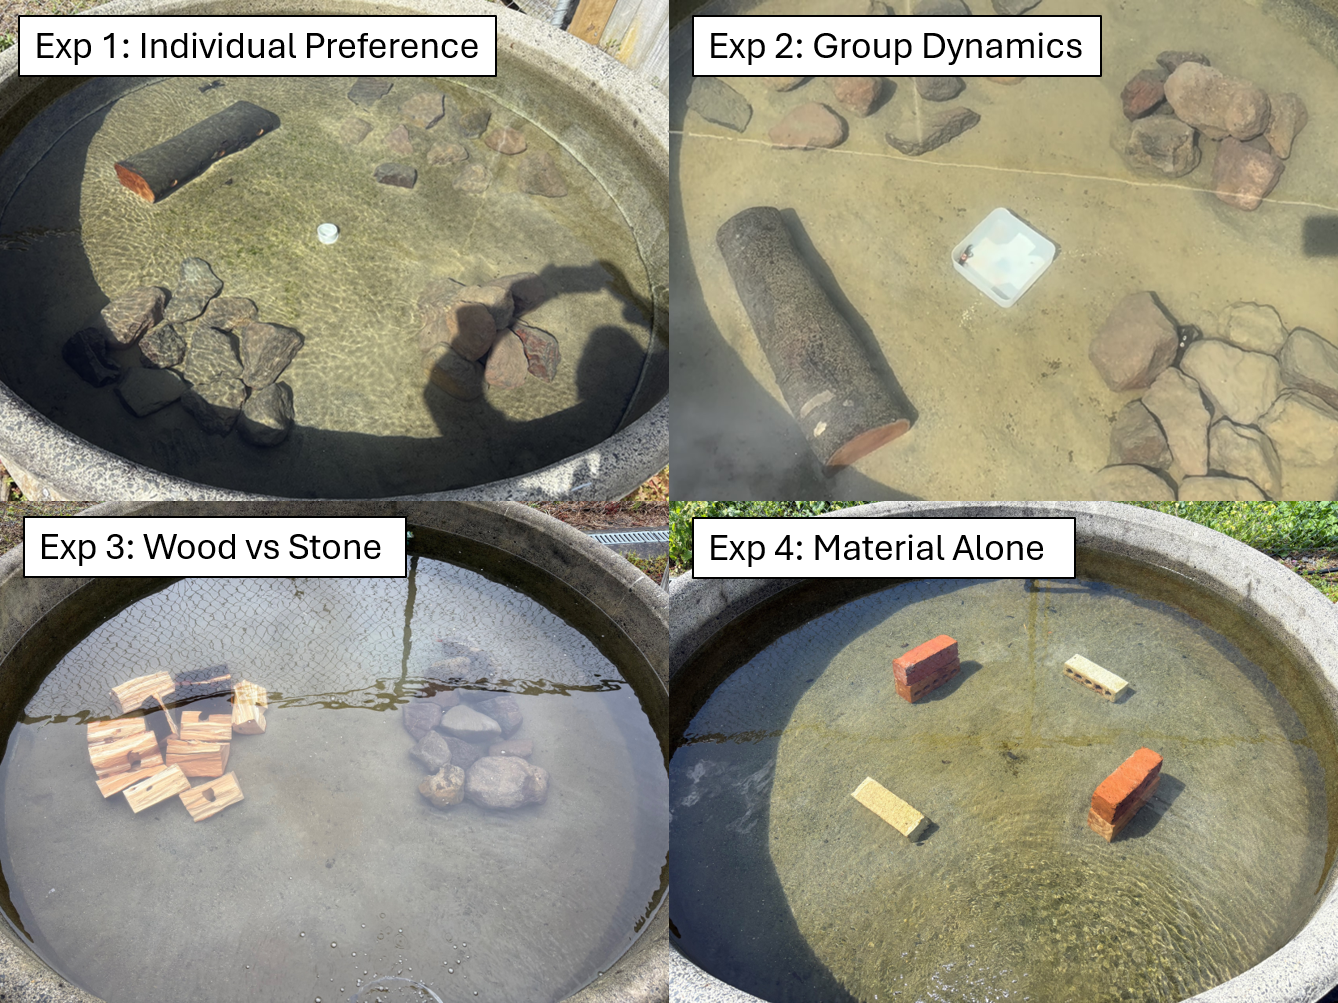
\includegraphics[width=1\linewidth,height=\textheight,keepaspectratio]{images/Setup_exp_tanks.png}

}

\caption{\label{fig-exp-setup}Overhead photographs of experimental tank
configurations for each of the four mesocosm experiments. Experiment 1
(Individual preference) and Experiment 2 (Group dynamics): four shelter
types, WoodLog (tānekaha log with drilled holes), FlatStone (stones
arranged flat), StonePile (stones stacked), and SingleStone (individual
stones placed separately). Experiment 3 (Wood vs Stone): WoodSplit
shelter (tānekaha wood splits) and FlatStone shelter placed in opposing
halves of the tank. Experiment 4 (Material comparison): ConcreteBrick
(perforated concrete bricks) and WoodBlock (perforated wooden blocks of
identical dimensions) placed in opposing quadrants of the tank.}

\end{figure}%

\subsection{Data analysis}\label{data-analysis-1}

Experiment 1: To test the difference between the four structure types
selected by the single kōura, a multinomial goodness-of-fit test was
performed using the XNomial package (Engels 2014). TankWall was excluded
from preference tests as it represents the absence of structure choice
rather than a structure type preference. Additionally, pairwise
likelihood-ratio G-tests with Bonferroni correction were used to
identify which structure types differed significantly from each other.
Bayesian categorical mixed-effects models were used to test whether body
size or sex affected structure preference across all experiments, fitted
using the brms package (Bürkner 2017, 2018). For Experiments 1 and 2,
where kōura chose among four structure types, a categorical family was
used. For Experiments 3 and 4, where only two structure types were
directly compared, a Bernoulli family was used. Model convergence was
assessed using the Gelman-Rubin diagnostic (all \(\hat{R}\) = 1.00) and
divergent transition counts (all experiments: 0 divergences), confirming
reliable posterior sampling (Gelman and Rubin 1992). To test whether
structure type use differed between sexes, the Bayesian categorical
mixed-effects model was fitted with structure type as the outcome, sex
as a fixed effect and tank and experimental round as random intercepts.
A permutation-based symmetry test was applied to assess whether
structure type transitions between initial location and next-day
location were directional rather than random.

Experiment 2: To test whether overall structure preference existed at
the group level, one-sample Wilcoxon signed-rank tests were applied to
group-round proportions for each structure type, testing against a null
expectation of 0.25 (equal distribution among four structure types).
P-values were Bonferroni adjusted for multiple comparisons. Normal
approximation was used due to ties arising from discrete group counts.
To test whether size classes affected structure preference while
accounting for repeated measurement of individuals and groups, the
Bayesian categorical mixed-effects model was fitted with structure type
as the outcome, size class as a fixed effect, and group identity,
individual identity nested within group, and tank and experimental round
as random intercepts. The Stuart-Maxwell test was used to test for
statistical differences between initial and next-day location.

Experiment 3: To test the difference between FlatStone and WoodSplit the
Wilcoxon signed-rank test was applied to group-round proportions for
each structure type, testing against a null expectation of 0.5. P-values
were Bonferroni adjusted. To test whether size classes affected
structure preference while accounting for repeated measurement of
individuals and groups, the Bayesian Bernoulli mixed-effects model was
fitted with size class as a fixed effect, following the same random
effects structure as described for Experiment 2. The Stuart-Maxwell test
was used to test for statistical differences between initial and
next-day location.

Experiment 4: To test whether kōura showed a preference between
ConcreteBrick and WoodBlock, the Wilcoxon signed-rank test was applied
to group-round proportions for each structure type, testing against a
null expectation of 0.5 and p-values were Bonferroni adjusted. A paired
Wilcoxon signed-rank test was used to directly compare group-round
proportions between ConcreteBrick and WoodBlock. As size class was
unbalanced, the effect of sex on structure preference was tested using
the Bayesian Bernoulli mixed-effects model with sex as a fixed effect,
following the same random effects structure as described for Experiment
2. Finally, as only next-day locations were recorded in this experiment,
no directional shift analysis was performed.

\section{Results}\label{results-2}

\subsection{Experiment 1: Individual
preference}\label{experiment-1-individual-preference-1}

Individual kōura showed a strong preference for WoodLog, selecting it
significantly more often than SingleStone, FlatStone, and StonePile
(pairwise G-test, Bonferroni adjusted: \emph{p} \textless{} 0.001,
0.011, 0.004, respectively; overall multinomial test: \emph{p}
\textless{} 0.001; Figure~\ref{fig-exp1}). No significant differences
were found among the stone structure types. Overall, WoodLog was
selected by 67 \% of kōura at refuge (males: 80 \%; females: 53 \%), and
no kōura were found at TankWall. Sex had no credible effect on structure
preference (\(\beta\) = 3.32, 95\% CI: -1.09 to 9.3; posterior
probability = 0.92) with credible intervals spanning zero for all
structure types. The symmetry test indicated that structure type use
shifted between initial and next-day location (\emph{p} \textless{}
0.001), suggesting kōura actively relocated to preferred structure types
overnight rather than remaining at their initial location. The video
footage showed kōura emerging, walking and climbing on the structures
after sunset.

\begin{figure}

\centering{

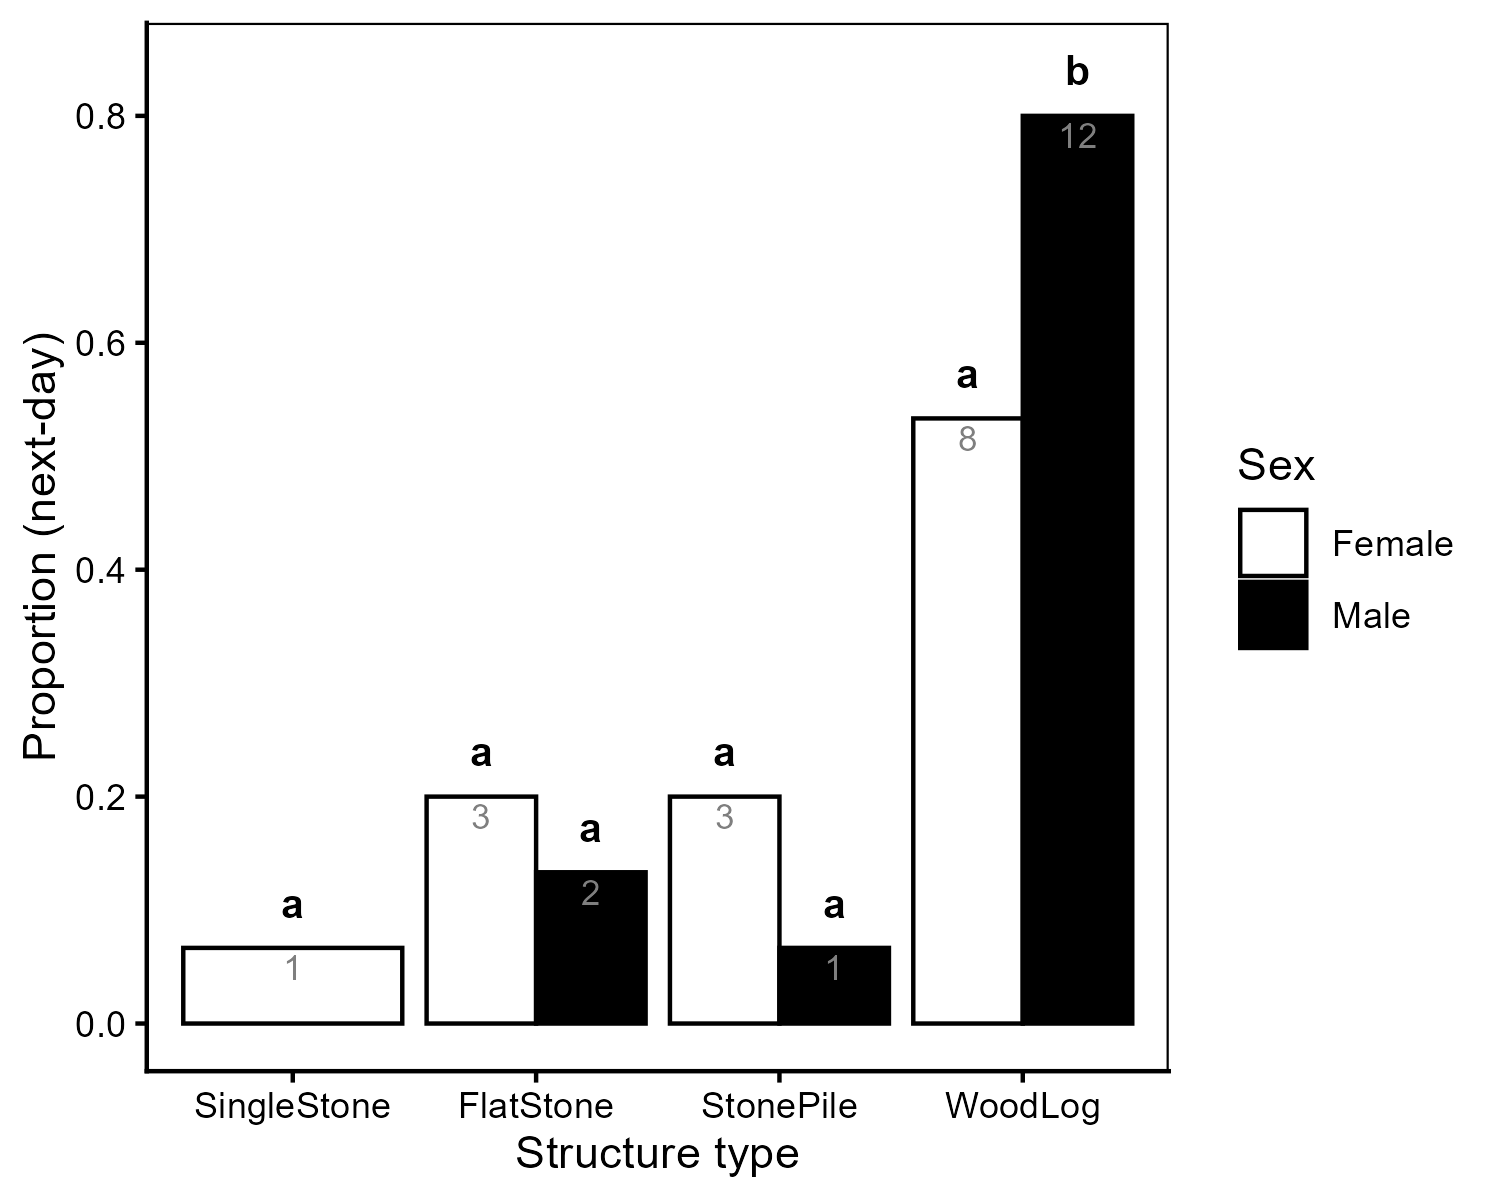
\includegraphics[width=0.65\linewidth,height=\textheight,keepaspectratio]{outputs/fig-exp1.png}

}

\caption{\label{fig-exp1}Proportion of individual kōura (Experiment 1)
found at each structure type the next day, shown separately for female
(white bars) and male (black bars) kōura. Bars show observed proportions
with sample sizes (n) shown on bars. Letters above bars indicate results
of pairwise G-tests with Bonferroni correction within each sex group,
structure types sharing the same letter within a panel do not differ
significantly from each other, while structure types with different
letters differ significantly in use. No significant difference in
overall structure preference was detected between sexes (see results).}

\end{figure}%

\subsection{Experiment 2: Group
dynamics}\label{experiment-2-group-dynamics-1}

When housed in mixed-size groups, kōura showed a significant overall
preference for stone-based structures (Figure~\ref{fig-exp2}). FlatStone
was used significantly more (\emph{p} = 0.004), while SingleStone
(\emph{p} \textless{} 0.001) and WoodLog (\emph{p} = 0.039) were
significantly avoided. StonePile did not differ from random expectation
(\emph{p} = 1.000) and did not differ significantly from FlatStone
(\emph{p} = 0.117). No kōura were found at TankWall, indicating active
structure selection across the group. Size classes had limited but
credible effect on structure preference. Medium-sized kōura showed a
weaker preference for FlatStone over SingleStone compared to small kōura
(\(\beta\) = -1.77, 95\% CI: -3.7 to -0.14; posterior probability =
0.99), while no other size class effect was credible. Overall, FlatStone
remained the most selected structure type across all size classes, but
its strength of preference declined from small (posterior probability of
top choice = 82 \%) to medium (53 \%), and with large kōura showing
similar preference between FlatStone and StonePile (42 \% vs 38 \%).
Structure type use shifted directionally between initial and next-day
location (Stuart-Maxwell test: \emph{p} = 0.001), indicating that kōura
actively relocated to preferred structure types overnight.

\begin{figure}

\centering{

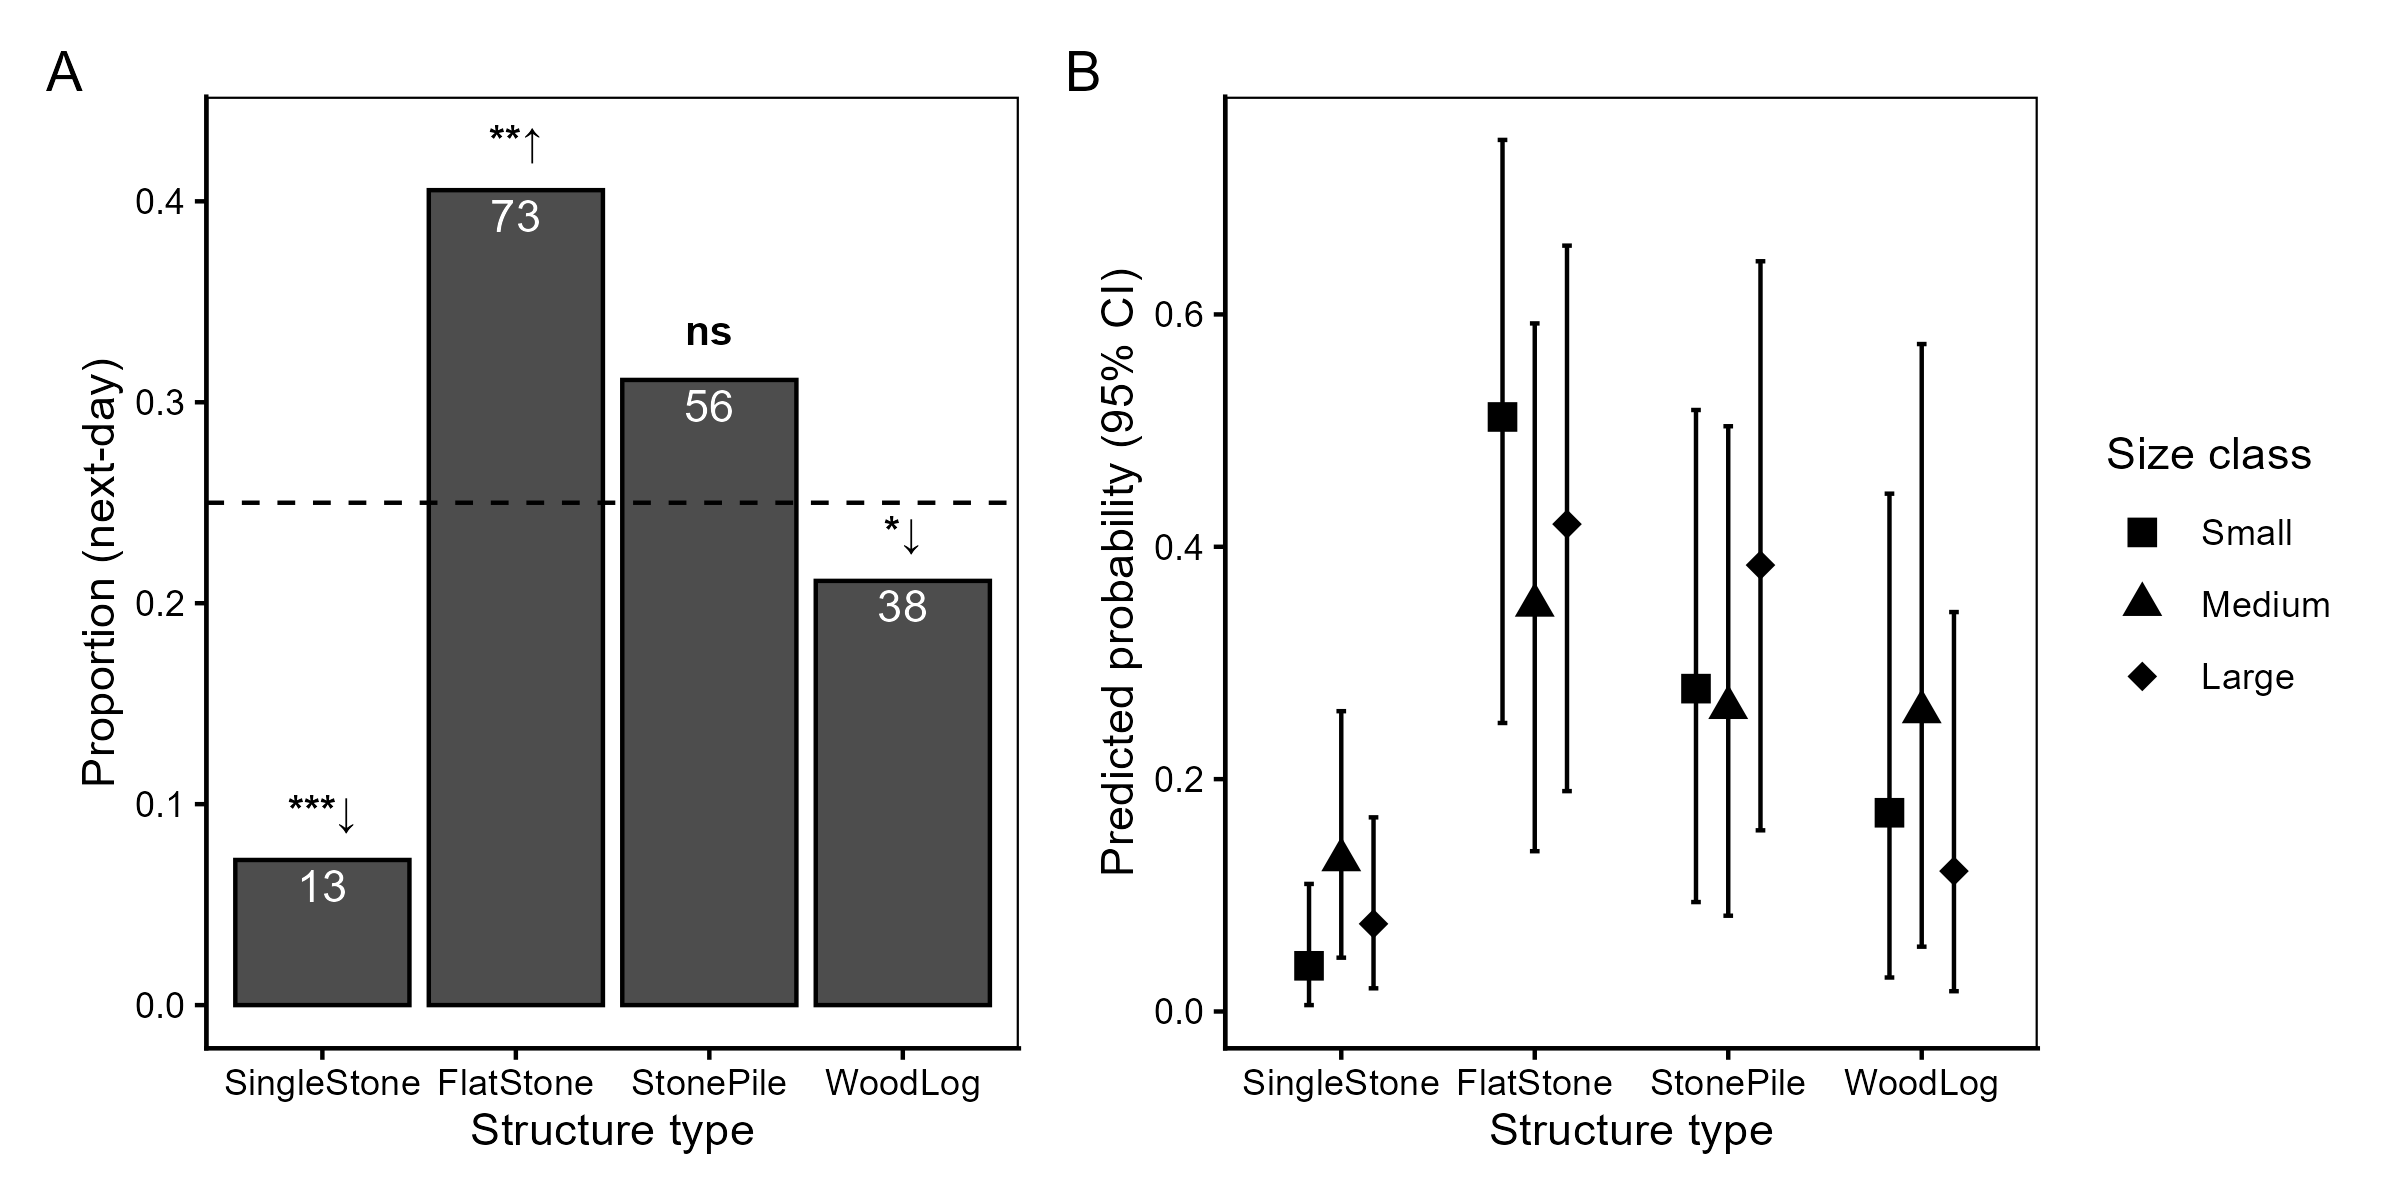
\includegraphics[width=0.8\linewidth,height=\textheight,keepaspectratio]{outputs/fig-exp2.png}

}

\caption{\label{fig-exp2}Structure type preference of group kōura
(Experiment 2). (A) Proportion of kōura found at each structure type at
L1 across all groups and rounds. The dashed line indicates the null
expectation of equal distribution (0.25). Significance symbols indicate
deviation from null expectation (Wilcoxon signed-rank test, Bonferroni
adjusted): \(\uparrow\) used more than expected, \(\downarrow\) used
less than expected. Sample sizes shown in white. (B) Posterior predicted
probability of structure type use by size class from Bayesian
categorical mixed model, with 95 \% credible intervals.}

\end{figure}%

\subsection{Experiment 3: Wood vs
Stone}\label{experiment-3-wood-vs-stone-1}

Kōura consistently selected FlatStone over WoodSplit, with the
preference growing with body size (Figure~\ref{fig-exp3}). At the group
level, FlatStone was used significantly more than expected (\emph{p} =
0.001), while WoodSplit was significantly avoided (\emph{p} = 0.004).
Only one kōura was found at TankWall. The Bayesian model indicated that
preference for FlatStone strengthened with body size, with the posterior
probability of FlatStone being the top-ranked structure increasing from
small (66 \%) to medium (79 \%), to large kōura (99 \%). Large kōura
showed a particularly strong and credible preference for FlatStone over
WoodSplit (\(\beta\) = -2.55, 95\% CI: -4.7 to -0.9; posterior
probability = \textgreater{} 0.99), while medium kōura did not differ
from small kōura. Structure type use shifted directionally between
initial and next-day location (Stuart-Maxwell test: \emph{p} = 0.003),
with kōura relocating toward FlatStone overnight.

\begin{figure}

\centering{

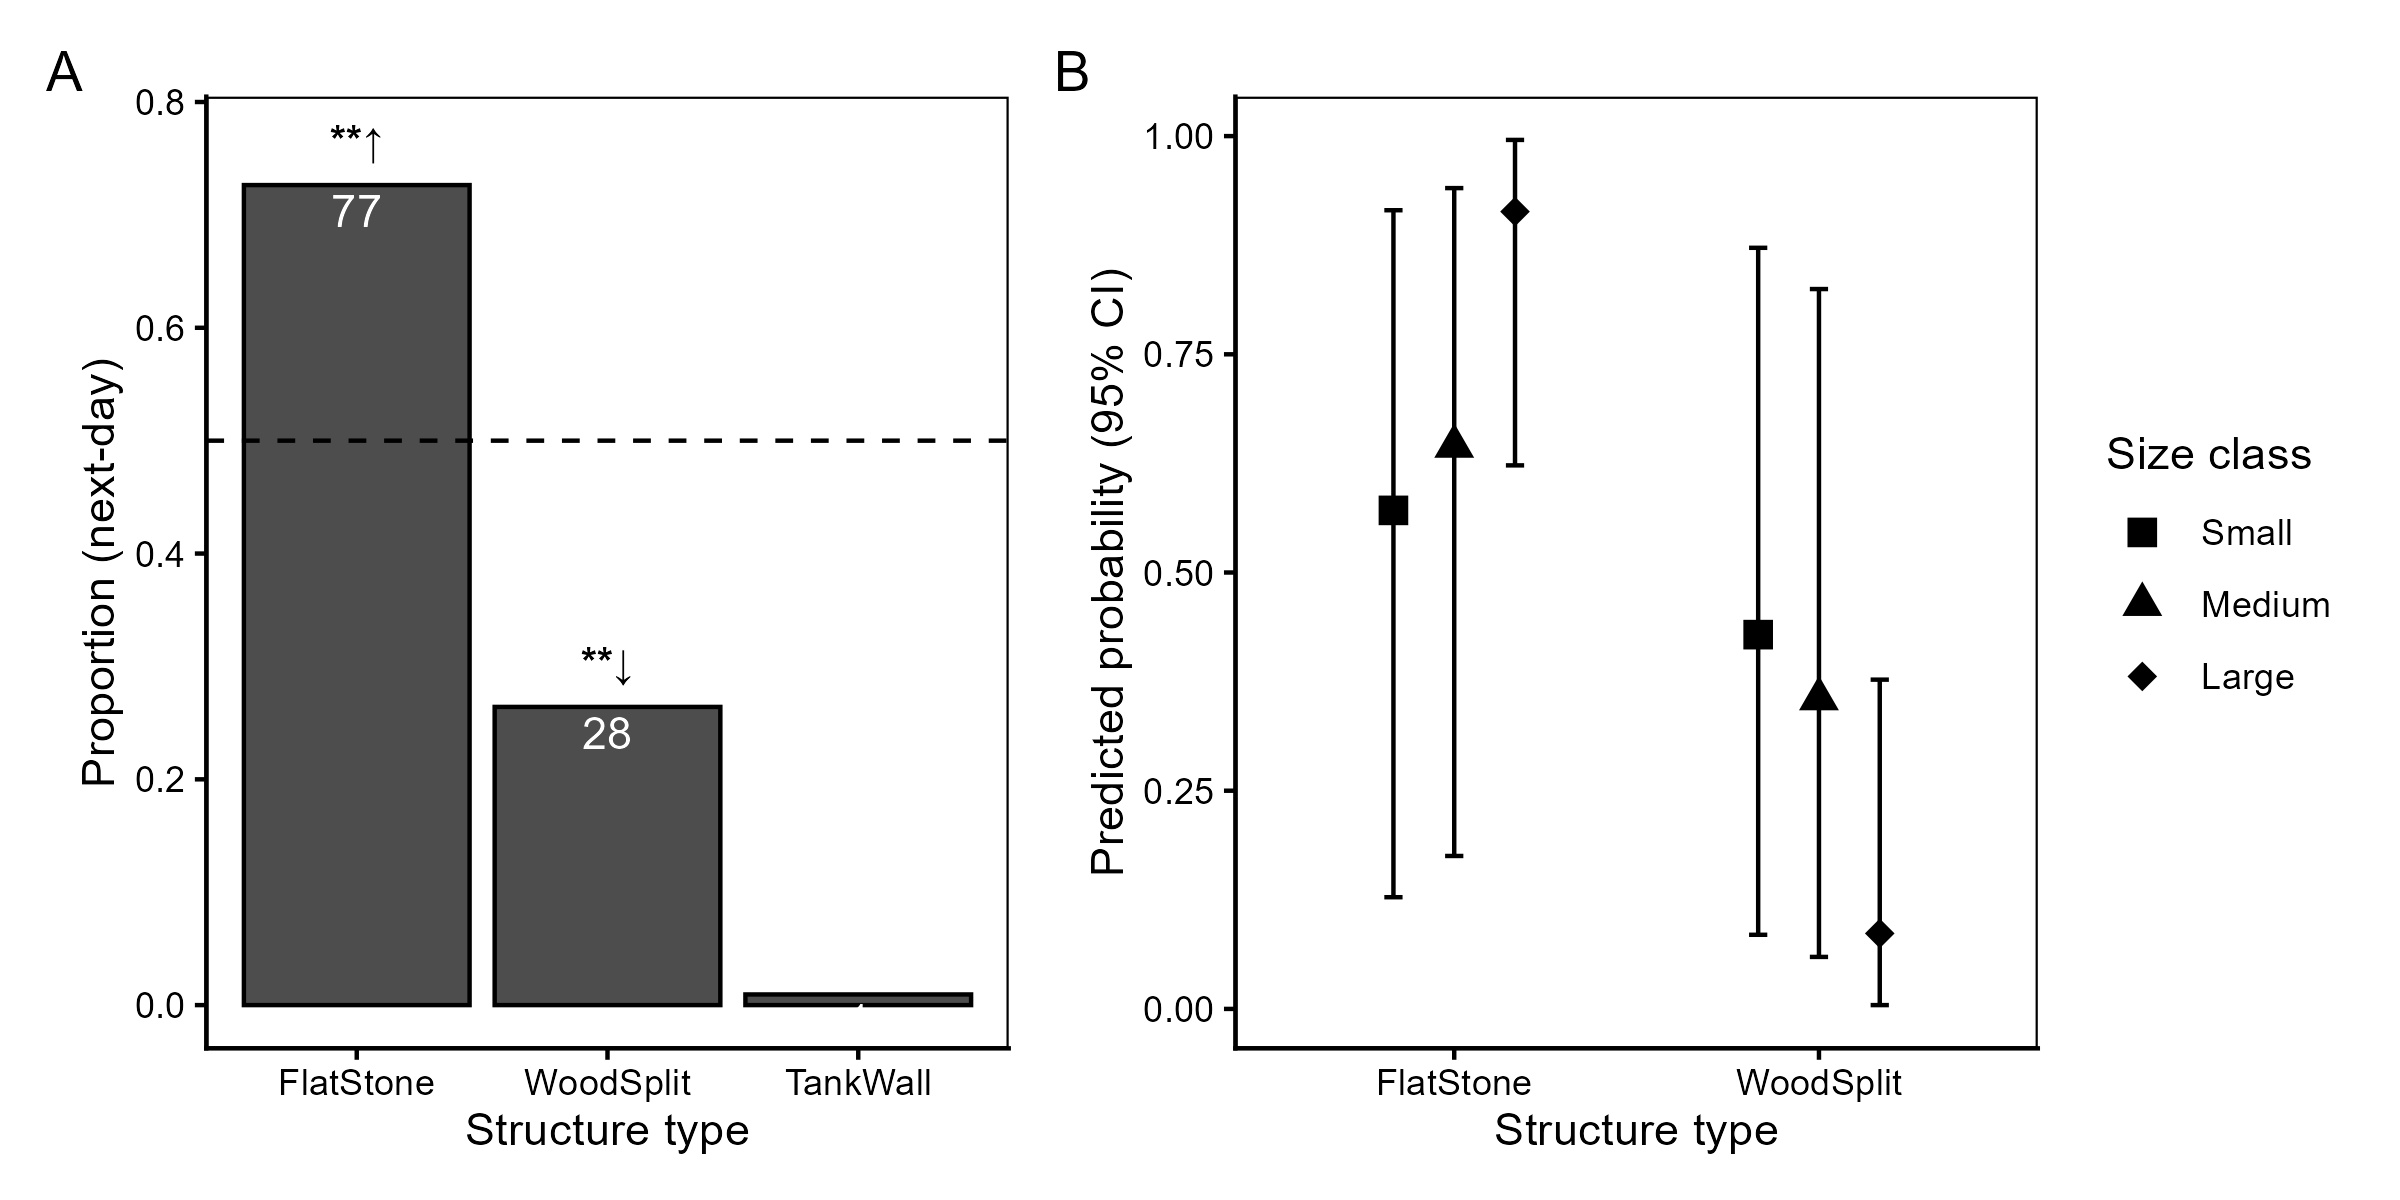
\includegraphics[width=0.8\linewidth,height=\textheight,keepaspectratio]{outputs/fig-exp3.png}

}

\caption{\label{fig-exp3}Structure type preference in stone versus wood
comparison (Experiment 3). (A) Proportion of kōura found at each
structure type at next-day location across all groups and rounds. The
dashed line indicates the null expectation of equal distribution (0.5).
Significance symbols as in Figure 3. (B) Posterior predicted probability
of structure type use by size class from Bayesian categorical mixed
model, with 95 \% credible intervals. \(\uparrow\) used more than
expected, \(\downarrow\) used less than expected. TankWall excluded from
model predictions.}

\end{figure}%

\subsection{Experiment 4: Material
comparison}\label{experiment-4-material-comparison-1}

Kōura used both structure types, showing no significant preference
between ConcreteBrick and WoodBlock (\emph{p} = 0.137;
Figure~\ref{fig-exp4}), with mean group proportions of 47 \% and 53 \%
respectively. Neither structure type differed significantly from equal
distribution (\emph{p} = 0.273). 9 \% of kōura were found at TankWall,
which is higher than in any previous experiment, likely reflecting the
smaller total structure size in this experiment rather than active
structure avoidance. Sex had no credible effect on preference between
structure types (\(\beta\) = -0.18, 95\% CI: -1.24 to 0.84; posterior
probability = 0.65), indicating that both structures were equally
suitable refuge for male and female kōura.

\begin{figure}

\centering{

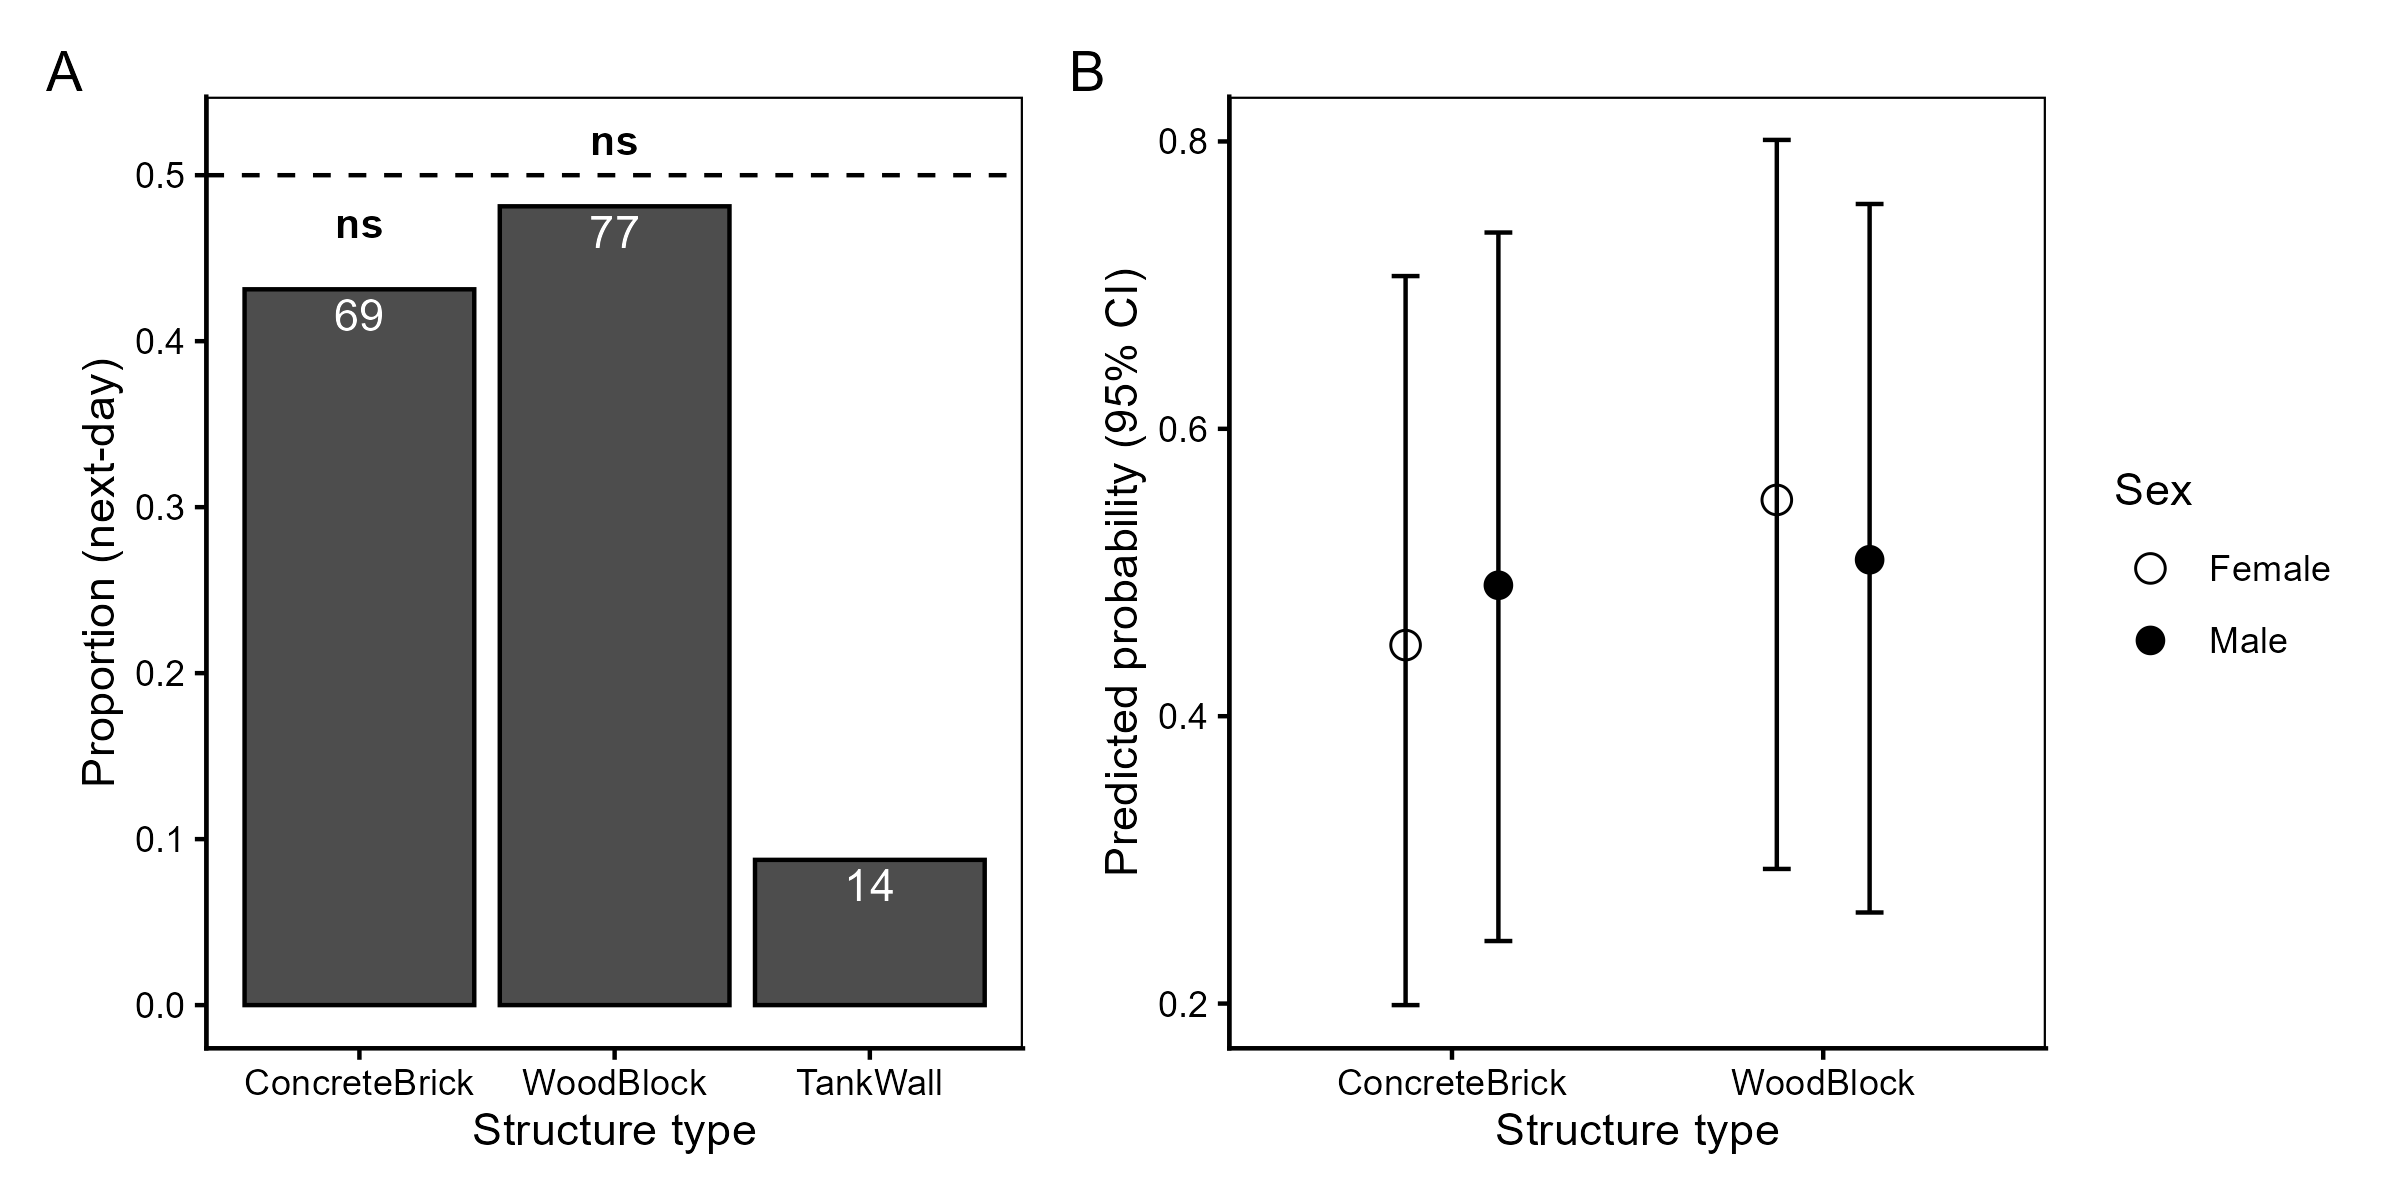
\includegraphics[width=0.8\linewidth,height=\textheight,keepaspectratio]{outputs/fig-exp4.png}

}

\caption{\label{fig-exp4}Material preference (Experiment 4). (A)
Proportion of kōura found at each structure type at next-day location
across all groups and rounds. The dashed line indicates the null
expectation of equal distribution (0.5). (B) Posterior predicted
probability of structure type use by sex from Bayesian categorical mixed
model, with 95 \% credible intervals. TankWall excluded from model
predictions.}

\end{figure}%

\section{Discussion}\label{discussion-2}

\subsection{Structure matters more than
material}\label{structure-matters-more-than-material}

The consistent finding across all experiments that structural stability
and cavities complexity determined preference, regardless of whether the
comparison involved material type, configuration or group size, suggests
that kōura, like many refuge-dependent crustaceans (Zimmer-Faust and
Spanier 1987; Beck 1995; Streissl and Hödl 2002; Pirtle et al. 2012),
are primarily selecting for physical shelter quality rather than
material familiarity. When hole dimensions were held constant between
concrete and wooden perforated structures, no preference for either
material was detected, demonstrating that material composition alone may
not drive refuge selection when structure is equivalent. Neither
structure type was conditioned prior to experiments, meaning biofilm
colonisation that occurs in natural lake environments was absent. As
stone and wood develop different biofilm communities (Tank and
Winterbourn 1996), material preference in field settings could change.
The wooden structures required a clay brick placed on top to prevent
floating, creating a difference with the concrete structures, though the
absence of any preference suggests this did not meaningfully influence
the result. This material-independence broke down when material affected
structural properties: when flat-laid stones were compared against
similarly sized split wood pieces, kōura showed a clear preference for
stone. The wood splits, being less dense than stone, sank but created
less structurally stable refuge places in the sandy substrate than the
stones, as larger kōura were able to move them {[}O.V. Raven, pers.
obs.{]}.

In group settings, structures providing the most crevice complexity were
strongly preferred, with flat-laid stones accommodating the most kōura,
followed by stone piles. Individual kōura showed a different preference,
consistently choosing the perforated wooden log over all stone options,
which is consistent with our first prediction that structurally complex
and enclosed refugia would be preferred as enclosed spaces reduce
predation risk (Jurcak et al. 2016). The individual drilled holes in the
wooden log offered protection similar to what has been found for
perforated brick and PVC tube shelters in response to the threat of
catfish predation (Adams 2007; Zhao et al. 2024). The directional shift
in structure type use, between initial locations shortly after release
and their location following a night within the tank, confirmed across
all experiments that kōura actively relocated overnight, supporting the
interpretation that next-day locations reflect genuine refuge preference
rather than chance displacement.

The shift from the perforated wooden log in individual trials to stone
structures in group trials was unexpected. The wooden log contained six
individual drilled holes, so capacity was not limiting for the group of
six kōura. The preference shift may partly reflect size mismatch between
fixed hole dimensions, and the range of body sizes present in each
group, with only medium-sized individual finding the holes well-suited,
while small and large individuals were better served by the range of
crevices created by the stone structures (Streissl and Hödl 2002).
However, a more fundamental explanation may relate to social behaviour.
The wooden log was the most selected structure in round 1 of Experiment
2 (17 out of 36 times), similar to Experiment 1, but this preference did
not persist in subsequent rounds. This shift suggests that once kōura
had experienced sharing the tank, they adjusted their shelter use toward
structures allowing closer conspecific proximity. Gregarious shelter
behaviour has been documented in juvenile burrowing crayfish (Hazlett et
al. 2007; Reynolds et al. 2013; Clay et al. 2017) and is well
established in lobsters including the New Zealand rock lobster
(\emph{Jasus edwardsii} Hutton, 1875) (Butler et al. 1999), where
conspecific chemical cues attract individuals to share refugia and find
refugia significantly faster, reducing predation exposure (Zimmer-Faust
and Spanier 1987; Childress and Herrnkind 2001). Whether kōura exhibit
similar gregarious tendencies remains understudied, but the preference
shift observed in this study, might suggest that social context alters
shelter preferences.

\subsection{Body size and competitive
dynamics}\label{body-size-and-competitive-dynamics}

Size class consistently influenced refuge preference across experiments,
but the pattern differed by context. In Experiment 3, larger kōura
showed a stronger preference for flat stones over wooden splits than
smaller individuals, consistent with size dependent shelter selection
documented in crayfish (Streissl and Hödl 2002; Percival and Moore
2010). This may reflect larger kōura being more capable of asserting
dominance over preferred stable refugia through competitive
displacement, which is consistent with the size-based dominance
hierarchy documented in kōura populations (Ranta and Lindström 1993;
Figler et al. 2005; Stewart and Tabak 2011). In Experiment 2, where four
structure types were available, small kōura showed the strongest
preference for flat stones while large kōura distributed more evenly
between flat stones and stone piles, suggesting that the large
continuous surface area of the flat stones provides refuge spaces
proportional to smaller body dimensions (Streissl and Hödl 2002), while
larger individuals find adequate crevice space in either stone
configuration. The absence of sex effects in Experiments 1 and 4
suggests that refuge preference in kōura is driven primarily by body
size and competitive dominance rather than sex (Figler et al. 1999).
When refuge availability is limited, competitive hierarchies displace
smaller and recently moulted individuals from preferred refugia, leaving
them exposed (Ranta and Lindström 1993; Figler et al. 2005). Providing
sufficient refuge spaces with a range of crevice size can reduce
agonistic interactions and benefit the whole population (Olsson and
Nyström 2009), supporting complex structure configurations over
structures with fixed hole dimensions.

\subsection{Restoration implications}\label{restoration-implications}

With the threat from invasive predatory fish, such as catfish preying on
kōura (Kusabs et al. 2026), enhancing habitat complexity may reduce
top-down control on kōura populations. Additional habitat as used here
can provide shelter spaces and offers a promising management tool, as
refuge availability directly influences predation survival (Adams 2007;
Zhao et al. 2024). The present study demonstrates that structural
configuration and stability drive refuge preference more strongly than
material composition, with stone-based configurations preferred by
groups and no preference detected between materials when dimensions were
equal, suggesting that stone-based habitat enhancement structures
warrant field evaluation in lake environments.

The broader restoration literature supports both the structural
principle and the choice of natural materials. Structurally stable
crevices are important for freshwater species like crayfish (Huolila et
al. 1997; Streissl and Hödl 2002), but also for marine environments, as
reef fish, marine shrimp, and lobsters have all been shown to benefit
from habitat enhancement structures such as artificial reefs (Spanier
1994; Magnelia et al. 2008; Hylkema et al. 2020; Dickson et al. 2023).
Structures made from stone and wood have been shown to outperform
synthetic alternatives and bare substrates (Huolila et al. 1997;
Magnelia et al. 2008; Dickson et al. 2023; Cooke et al. 2023), and do
not contribute to plastic pollution in the environment (Cooke et al.
2023). Locally sourced natural materials also align with
\emph{kaitiakitanga}, which is the Māori principle of environmental
guardianship and preserves the natural character of culturally
significant lake environments (Clapcott et al. 2018). Furthermore,
existing habitat surveys suggest that kōura are associated with coarser
substrates (Olsson et al. 2006; Jowett et al. 2008; Kusabs et al.
2015b), and cobbles have previously been used in stream and lake
restoration (Huolila et al. 1997; Johnsen and Taugbøl 2008). For in-lake
deployment stone pile structures are likely to be the most practical
configuration, due to their elevated structure, stone piles are less
likely to be buried into soft substrates than flat individual rocks
(Garron et al. 2024). Field validation in lake environments remains an
essential next step, as in-lake conditions including water movement,
natural substrate, and predator pressure may modify kōura preferences in
ways not captured under controlled conditions.

\subsection{Conclusion}\label{conclusion}

Across four mesocosm experiments, structural configuration and crevice
complexity consistently predicted kōura shelter preference more strongly
than material composition. The shift from individual preference for
enclosed wooden log shelters to group preference for stone
configurations shows that social context plays a key role in determining
shelter value for kōura. Size-dependent preferences further suggest that
structures accommodating multiple body sizes simultaneously benefit
whole populations rather than only dominant individuals. Stone-based
structures using locally sourced materials are promising candidates for
field evaluation, aligning with ecological and cultural values
associated with restoring this taonga species. Field validation remains
the essential next step for translating these findings into effective
kōura habitat restoration practice.

\section{Acknowledgements}\label{acknowledgements-3}

We thank Te Arawa Lakes Trust and Te Komiti Whakahaere for the
opportunity to collect and study the treasured kōura. We are grateful to
Soweeta Fort-D'ath and William Anaru (Te Arawa Lakes Trust), and Tihini
Grant (Ngāti Pikiao).

\clearpage
\providecommand{\chaptermark}[1]{}
\ifcsname c@chapter\endcsname
\setcounter{chapter}{5}
\setcounter{figure}{0}
\setcounter{table}{0}
\setcounter{section}{0}
\addcontentsline{toc}{chapter}{\protect\numberline{5}Rock Piles as K\={o}ura Habitat}
\chaptermark{Rock Piles as K\={o}ura Habitat}
\fi
\providecommand{\thechapter}{5}
\thispagestyle{empty}
\begin{tikzpicture}[remember picture, overlay]
  \begin{scope}
    \clip ([yshift=-7cm]current page.north west)
          rectangle ([yshift=4.5cm]current page.south east);
    \node[inner sep=0pt, anchor=north]
      at ([yshift=-7cm]current page.north)
      {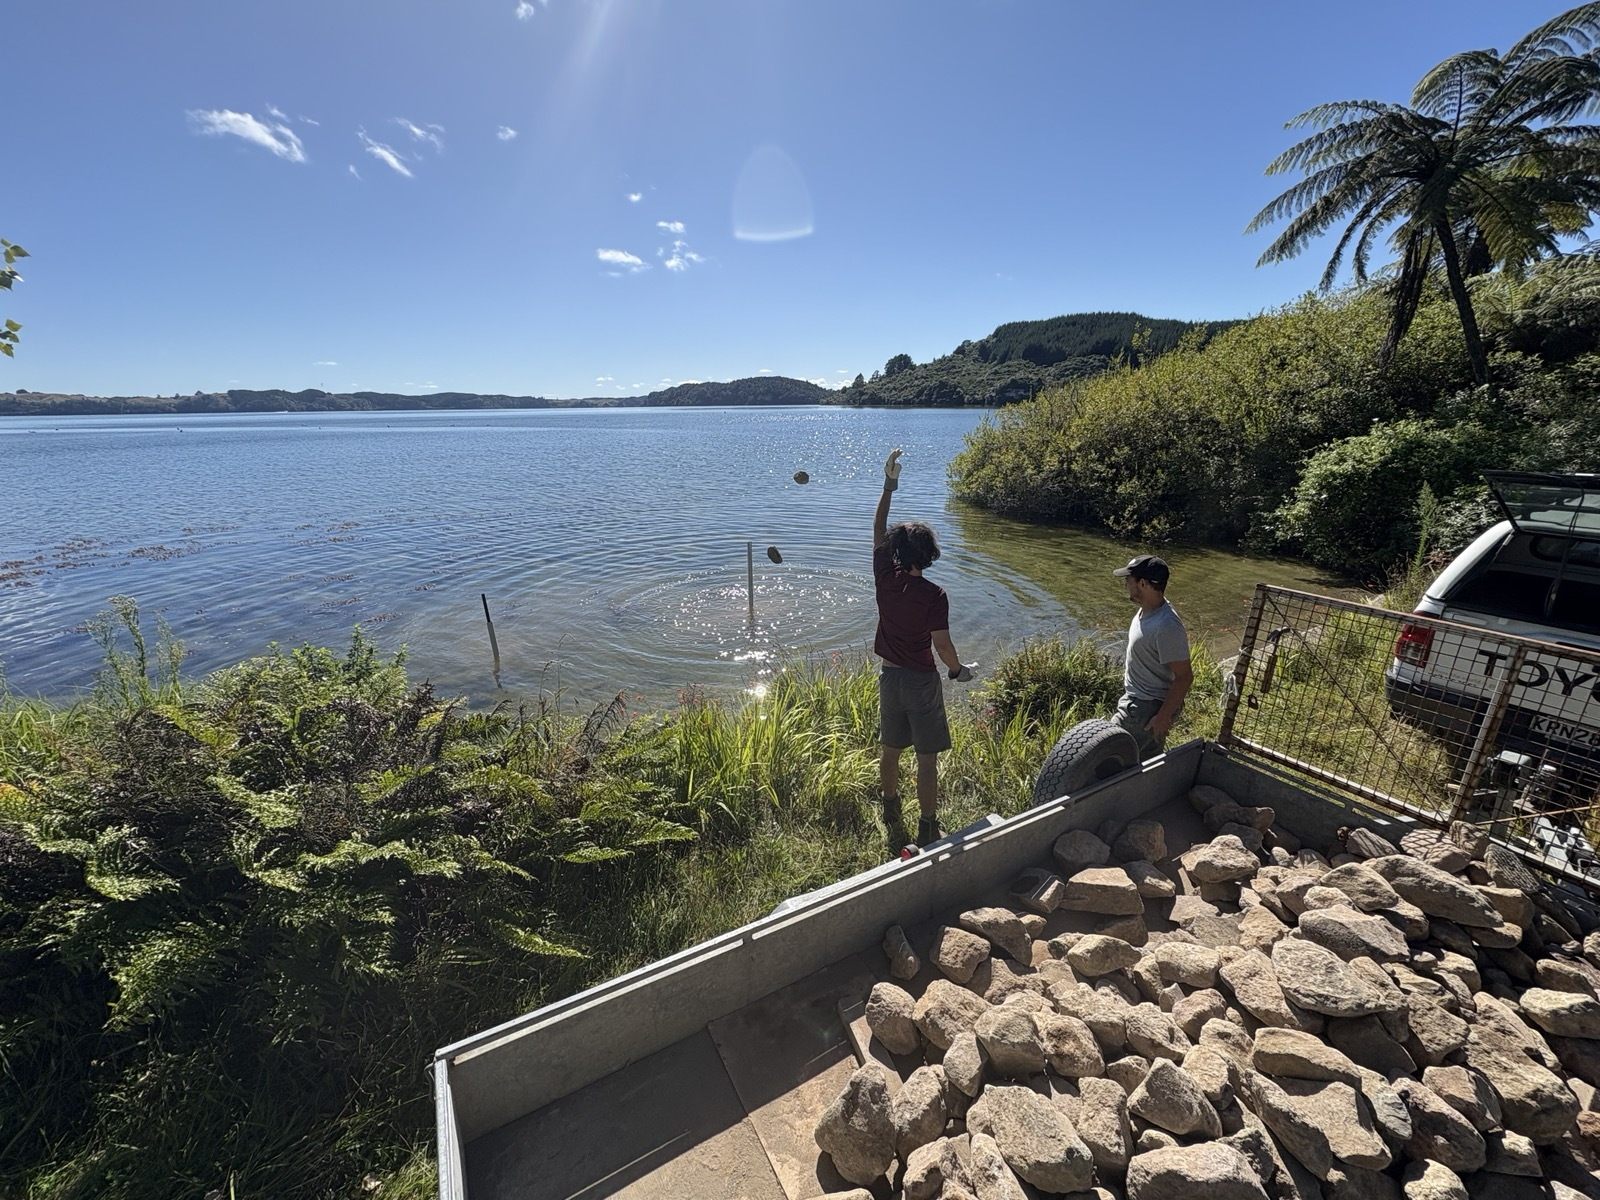
\includegraphics[height=18.2cm]{images/ch5_cover.jpg}};
  \end{scope}
  \fill[black]
    (current page.north west) rectangle ([yshift=-7cm]current page.north east);
  \node[color=thesissand, align=left,
        font=\fontsize{13}{16}\selectfont\sffamily, anchor=west]
    at ([xshift=1.5cm, yshift=-1.5cm]current page.north west)
    {Chapter \thechapter};
  \node[color=white, text width=0.85\paperwidth, align=left,
        font=\fontsize{22}{28}\selectfont\bfseries\sffamily, anchor=west]
    at ([xshift=1.5cm, yshift=-4cm]current page.north west)
    {Rock Piles as K\={o}ura Habitat};
  \node[color=white, text width=0.85\paperwidth, align=left,
        font=\fontsize{10}{13}\selectfont\itshape\sffamily, anchor=north west]
    at ([xshift=1.5cm, yshift=-5.0cm]current page.north west)
    {Habitat enhancement for a native freshwater crayfish threatened by an invasive predator: a field trial of stone pile structures in an Aotearoa New Zealand lake};
  \fill[black]
    (current page.south west) rectangle ([yshift=4.5cm]current page.south east);
  \node[color=white, text width=0.85\paperwidth, align=left,
        font=\fontsize{9}{13}\selectfont\sffamily, anchor=west]
    at ([xshift=1.5cm, yshift=3.2cm]current page.south west)
    {Olivier V.\ Raven, Ian A.\ K.\ Kusabs, Robin Holmes, Francis J.\ Burdon \& Deniz Özkundakci};
  \node[color=thesissand, text width=0.85\paperwidth, align=left,
        font=\fontsize{9}{13}\selectfont\itshape\sffamily, anchor=west]
    at ([xshift=1.5cm, yshift=1.5cm]current page.south west)
    {Journal of Applied Ecology--- In preparation};
\end{tikzpicture}
\null
\clearpage

\section*{Abstract}\label{abstract-4}
\addcontentsline{toc}{section}{Abstract}

\begin{enumerate}
\def\labelenumi{\arabic{enumi}.}
\tightlist
\item
  Kōura (\emph{Paranephrops planifrons}), Aotearoa New Zealand's endemic
  freshwater crayfish, have declined by up to 96 \% in Lake Rotoiti (Te
  Arawa Lakes, Rotorua), driven by predation from the invasive brown
  bullhead catfish and by thermal stratification and invasive
  macrophytes that compress suitable habitat into the shallow littoral
  zone. Because these stressors cannot be removed at the lake scale,
  adding structural refuge may be one of few practical management
  options.
\item
  We tested whether stone pile structures deployed in the littoral zone
  of Lake Rotoiti could provide structural refuge for kōura from
  predation. Kōura and catfish were monitored at five stone piles, five
  control, and five paired natural rocky reference sites for 18 months
  using a quasi before-after control-impact (quasi-BACI) design, with
  kōura occupancy modelled using a Bayesian framework that incorporated
  detection probabilities from baited traps and fyke nets.
\item
  Stone pile construction produced no statistically significant change
  in kōura abundance, biomass, or occupancy relative to controls, but
  effects consistently trended positive across models; a
  simulation-based power analysis showed the study was underpowered to
  detect the observed effect size, given high pre-construction occupancy
  (81--89\%) at all site types and only five site pairs.
\item
  Kōura use of stone piles was strongly seasonal: catch rates at stone
  pile and control sites fell in winter as kōura withdrew to deeper
  water, while reference sites remained stable. Catfish showed no
  comparable attraction to stone piles in any season or model.
\item
  Synthesis and applications. Stone piles show early, consistent
  evidence of benefiting a threatened native crayfish without benefiting
  its invasive predator, and are most valuable when habitat compression
  and predation pressure peak together in summer and autumn ---
  conditions expected to intensify under climate warming. This study
  establishes a tested, scalable construction and consenting methodology
  that lake managers can deploy as an interim refuge-based tool while
  catfish eradication remains unachievable at the lake scale; we
  recommend continued monitoring beyond three years and trialling
  connected, corridor-style structures rather than isolated piles.
\end{enumerate}

\section{Introduction}\label{introduction-3}

Freshwater biodiversity is declining faster than any other biome, with
one quarter of freshwater fauna now threatened with extinction (Sayer et
al. 2025). Among the most endangered are freshwater crayfish, with 32\%
of species assessed as threatened globally due to habitat loss, invasive
species, and declining water quality (Richman et al. 2015). As keystone
species and ecosystem engineers, crayfish play crucial roles in nutrient
cycling, bioturbation, and food web dynamics, and their loss can have
cascading consequences for freshwater ecosystems (Momot 1995; Collier et
al. 1997; Parkyn et al. 2001). In Aotearoa New Zealand, these pressures
converge on kōura (\emph{Paranephrops planifrons} White, 1842), an
endemic freshwater crayfish now facing rapid population decline in lakes
that have long supported some of the largest customary kōura fisheries
in the country (Hiroa 1921; Kusabs and Quinn 2009).

Kōura populations in Lake Rotoiti, located in the Rotorua Te Arawa Lakes
region of the North Island of Aotearoa New Zealand (hereafter Aotearoa),
have declined by up to 96 \% over the past two decades (Kusabs et al.
2026). This collapse has virtually ended customary harvest practices for
Te Arawa iwi (Māori tribal group) who are hunga tiaki (traditional
custodians) of the lake (Kusabs et al. 2015a). The decline in kōura
numbers is driven by multiple interacting stressors that compound over
time in different parts of the lake (Lee et al. 2025; Kusabs et al.
2026). The invasive brown bullhead catfish (\emph{Ameiurus nebulosus}
Lesueur, 1819, hereafter catfish), confirmed in Lake Rotoiti in 2016
(Francis 2019; Grayling 2020), preys directly on kōura and suppresses
their foraging through non-consumptive `fear' effects (Raven et al.
2026a). Predation pressure from catfish is compounded by additional
stressors that constrain where in the lake kōura can seek refuge from
this invasive predator (Kusabs et al. 2026).

During the day, kōura shelter in complex rocky habitat and in deeper
water to avoid predation (Jowett et al. 2008; Kusabs et al. 2015b),
moving out of both at night to forage in the productive littoral zone
(Devcich 1979). The importance of deep-water refuge is shown in Lake
Taupō, where kōura persist at a depth even in the presence of catfish
because the lake remains oxygenated below the thermocline (Kusabs and
Taiaroa 2015; Verburg and Albert 2019). In Lake Rotoiti, this deep
refuge becomes anoxic during summer stratification and unavailable for
kōura, compressing the zone of liveable habitat into the shallow
littoral margins (Kusabs et al. 2026), precisely where catfish are most
active (Dedual 2002; Blanchfield et al. 2026). Dense beds of invasive
macrophytes further restrict kōura movement through this compressed zone
and intensify oxygen depletion during die-off events (Vincent et al.
1984; Hamilton et al. 2005; Kusabs and Quinn 2009). Catfish pressure and
thermal stratification are expected to only strengthen with predicted
climate scenarios (Woolway et al. 2021; Lee et al. 2025), making kōura
habitat compression and predation pressure progressively more severe.

The compression of suitable habitat and subsequent concentration of
kōura into the littoral zone makes the quality of nearshore lacustrine
habitats increasingly important for remaining populations. In stream
environments, kōura are positively associated with structurally complex
habitats including bank undercuts, woody debris, leaf litter, and coarse
substrates (Usio and Townsend 2000; Parkyn and Collier 2004; Jowett et
al. 2008; Parkyn et al. 2009). In lake environments, benthic substrate
characteristics are a stronger predictor of kōura distribution than
nutrient enrichment or predator abundance (Kusabs et al. 2015b), and
kōura are positively associated with coarse substrates and riparian
vegetation (Raven et al. 2026b). Coarse rocky substrate provides refugia
from predators and shelter during moulting (Streissl and Hödl 2002).
Experimental studies confirm that shelter availability directly reduces
catfish predation on crayfish (Adams 2007; Zhao et al. 2024), and kōura
increase refuge use in the presence of catfish compared to native
predators (Raven et al. 2026a), emphasising the importance of shelter
availability for kōura populations. Shelter availability is likely a
limiting factor for kōura in Lake Rotoiti, where the majority of the
shoreline is sandy with dense beds of introduced macrophytes and little
rocky structure. Adding rocky substrate to soft-bottomed lake areas has
been shown to significantly increase crayfish abundance (Johnsen and
Taugbøl 2008), and increasing structural complexity in streams improves
crayfish restocking success (Huolila et al. 1997). Deploying habitat
enhancement structures that add structural complexity in the littoral
zone could potentially be a practical way to restore kōura populations
in Lake Rotoiti.

In this study habitat enhancement structures in the shape of stone piles
were deployed along the shoreline of Lake Rotoiti to investigate the
ability of the structures in providing additional habitat for kōura to
live and hide from predators. Kōura presence, abundance, and biomass
were monitored at stone pile, control, and reference sites over 18
months. We predicted that kōura occupancy, abundance and biomass would
increase more rapidly at the stone pile sites than at control sites, as
intense catfish predation pressure in the littoral zone was expected to
compel kōura actively toward available refuge structures. We further
predicted that kōura abundance would continue to increase progressively
after construction, at least within the first 18 months, and that
catfish would instead show seasonal patterns of shoreline use rather
than a construction-driven trend (Barnes 1996; Dedual 2002; Blanchfield
et al. 2026). Finally, we predicted that stone pile sites would
progressively converge toward kōura densities observed at natural rocky
reference sites, and that catfish would not exhibit a similar pattern.

\section{Materials and Methods}\label{materials-and-methods-3}

\subsection{Study location and
construction}\label{study-location-and-construction}

Lake Rotoiti (-38.03, 176.42) is a warm monomictic mesotrophic lake
located in the Rotorua Te Arawa Lakes region of the North Island of
Aotearoa (34 km², maximum depth 128 m). The lake stratifies for
approximately nine months a year ({Figure~\ref{fig-lake-conditions}}),
with pronounced thermal stratification compressing oxygenated habitat
into the shallow littoral zone during summer and autumn. Since 2008,
nutrient-rich inflows from Lake Rotorua have been diverted toward the
Kaituna River via the Ōhau Channel diversion wall to improve water
quality in Lake Rotoiti (Hamilton et al. 2005; Prentice et al. 2026).
Lake level is regulated by a weir at the outlet of the Kaituna River,
providing a stable and controlled water level throughout the year.
Catfish are present throughout the lake but occur in particularly high
concentrations in Te Weta Bay on the Northwest side of the lake (Francis
2019). Five stone pile sites were selected alongside the lake shoreline
based on accessibility and landowner approval (Figure~\ref{fig-sites}).
At each stone pile site, a paired control site was established 50 m
along the shoreline, matched for habitat characteristics e.g., water
depth, substrate type and vegetation cover. Five naturally occurring
rocky shoreline locations, with each two monitoring sites 50 m apart
were selected as reference. In total, 20 sites of each 150 m² (15 × 10
m) were monitored seasonally over 18 months. Physical characteristics of
all sites are summarised in Table~\ref{tbl-site-overview}. Baseline
monitoring was conducted in February 2025 prior to stone pile
deployment, which occurred the following week. Stone piles were
constructed from locally sourced quarry rock (Manawahe Stone and Quarry,
\textasciitilde25 km from the lake) with a diameter ranging from 85 -
315 mm (mean = 173 mm). At each of the five stone pile sites, three
stone piles were arranged horizontally along the shoreline by hand from
the shore. Stone pile design was informed by mesocosm experiments
demonstrating kōura preference for enclosed stone structures
(unpublished data). Stone piles were positioned approximately 4.3 m from
shore at a mean depth of 0.49 m and with a mean area of 4.1 m².

\subsection{Monitoring}\label{monitoring}

Physical, chemical, and biological parameters were recorded at each site
during each monitoring round. Static site characteristics including
substrate composition, slope to depth contour, riparian vegetation,
overhanging tree cover, and wood cover were visually estimated during
baseline monitoring only, as these were not expected to change
substantially over the monitoring period. Substrate composition was
visually estimated by a single observer walking around each site and
using an underwater viewing chamber, categorising bedrock, boulders
(\textgreater256 mm), cobble (64--256 mm), gravel (2--64 mm), sand
(0.063--2 mm), mud (\textless0.063 mm), and organic matter (Wentworth
1922). A substrate index, that indicates suitability for koura, was
calculated from these estimates (Jowett and Richardson 1990; Jowett et
al. 2008):

\[
\begin{aligned}
\text{Substrate index} &= 0.08 \times \text{bedrock} + 0.07 \times \text{boulders} \\
&\quad + 0.06 \times \text{cobble} + 0.04 \times \text{gravel} + 0.03 \times \text{sand} \\
&\quad + 0.02 \times \text{organic matter} + 0.01 \times \text{mud}
\end{aligned}
\] Coarser substrates were assigned higher weights as they provide
greater interstitial pore space and stable structures used by kōura
(Usio and Townsend 2000; Nyström et al. 2006).

After stone pile construction, measurements of the size and dimensions
of each structure were taken. The post-construction substrate index for
stone pile sites was recalculated using each site's combined stone-pile
footprint area, expressed as a percentage of the 150 m² site area and
treated as 80 \% cobble and 20 \% boulders displacing an equivalent area
of sand, to reflect their contribution to substrate complexity. Slope
was assessed as the horizontal distance from the shoreline to the 20 m
depth contour, derived from bathymetric maps and measured in a projected
coordinate system (NZTM2000; EPSG:2193).

Seasonal variable parameters were recorded at every monitoring round and
included aquatic vegetation cover (emergent and submerged macrophytes).
Chemical parameters included water temperature (°C), dissolved oxygen
(mg L\(^{-1}\)), and conductivity (\(\mu\)S cm\(^{-1}\)) were measured
using a YSI ProSolo meter (Pro2030, YSI Inc., Yellow Springs, OH, USA).
pH was measured using a handheld pH meter (EC-PCTestr35, Eutech
Instruments).

Kōura and fish were sampled every monitoring round using two
single-winged, double-throated fyke nets (600 mm high D-shaped entrance
hoop) and two collapsible bait traps (480 × 250 mm; two 50 mm entrance
openings) baited with catfish flesh (Joy et al. 2013; MacNeil et al.
2025). Fyke nets were placed perpendicular to the shoreline outside of
the stone pile structures or at 10 m intervals, with bait traps
positioned between them. All equipment was deployed simultaneously at
each site for a 24-h period. Captured kōura were measured for orbital
carapace length (OCL) using a digital calliper (0.01 mm precision; 150
mm) and for wet mass using a digital scale (± 1 g; 5 kg capacity, Anko
Brand, Kmart Group, Mulgrave, VIC, Australia). Catfish and other fish
species, were recorded for abundance, measured for total length, and
weighed for wet mass. Catch per unit effort (CPUE) and biomass per unit
effort (BPUE) were calculated for all kōura and fish based on the number
of nets and traps deployed at each site per monitoring round,
standardised by soak time (Kusabs et al. 2015b). Kōura weights were
unavailable for 36 individuals because of scale failure and were
therefore estimated from a log₁₀--log₁₀ length--weight regression fitted
to individuals with both measurements (n = 840), following standard
approaches for weight length relationships in aquatic organisms
{Figure~\ref{fig-length-weight-ch5}} (Froese 2006). Predicted values
were back-transformed with a lognormal bias correction factor
\(10^{0.5 \sigma^2}\) (Quinn and Keough 2002).

\[
\log_{10}(\text{Weight [g]}) = -2.67 + 2.684 \times \log_{10}(\text{OCL length [mm]})
\]

\subsection{Data analysis}\label{data-analysis-2}

Data analysis was a three-part process, the first assessed baseline
equivalence between stone pile, control, and reference sites before
construction, the second assessed the impact of stone pile construction
and after-construction trajectory on kōura and catfish occupancy,
abundance, and biomass, and the third assessed whether stone pile sites
converged toward reference sites and if reference sites remained stable
over time. All analyses were conducted in R (version 4.6.1; R Core Team
(2026)) using the glmmTMB and emmeans packages (Brooks et al. 2017;
Lenth and Piaskowski 2017).

Covariate selection for all models followed a consistent procedure.
Corrected Akaike Information Criterion (AICc) values for each base model
were compared against models with additional covariates (temperature,
season, substrate index, maximum effective fetch, or wave energy proxy)
added at a time, and a covariate was retained only when it reduced AICc
by more than two units relative to base model (Burnham and Anderson
2002). Robustness and sensitivity for all models were assessed by
evaluating uniform distribution, dispersion and outlier rate using the
DHARMa package (Hartig 2016). Across the full set of models, the
Benjamini--Hochberg correction method was applied to control the false
discovery rate within each of the three analysis components.

Site variation before stone pile construction was assessed using paired
Wilcoxon signed-rank tests to compare stone pile sites with their paired
control sites, and unpaired Wilcoxon rank-sum tests to compare stone
pile sites with reference sites. This was done for response variables
(water quality, substrate, and kōura and catfish CPUE and BPUE) to
confirm that the stone pile and control sites were equivalent before
construction, and to characterise the difference between stone pile and
reference sites. To further assess baseline equivalence, generalised
linear models (GLMs) were fitted to test whether kōura and catfish CPUE
and BPUE differed between site type (stone pile / control) and between
the two reference sites (reference 1 / reference 2) using a Tweedie
family with a log link. Following the covariate selection procedure,
temperature was included in the catfish models comparing reference
sites, as the base model failed to converge and temperature was required
for numerical stability.

The second component of the analysis tested construction impact relative
to control sites using a quasi-before-after, control-impact (quasi-BACI)
design (Underwood 1994), and separately tested after-construction
trajectory of kōura and catfish populations. The quasi-BACI design
compared one pre-construction monitoring round with six
post-construction monitoring rounds using generalised linear mixed
effects models (GLMMs) to test the effect of stone pile construction on
kōura and catfish occupancy, abundance, and biomass. Time period (before
/ after) and site type (stone pile / control) were included as an
interaction term, monitoring round as a covariate and site nested within
control-impact pair as a random effect. Occupancy was modelled using a
binomial GLMM, and abundance and biomass using a Tweedie GLMM with a log
link; fetch was retained as a covariate in the catfish model. The
post-construction trajectory models used the same response variables,
families, covariate, and random effect structure, but with site type and
monitoring round included as an interaction term in place of the before
/ after comparison.

The third component of the analysis assessed whether stone pile sites
converged toward reference sites over time, and whether reference sites
themselves remained stable. Kōura and catfish abundance and biomass were
tested using GLMMs with site type (stone pile / reference) and
monitoring round included as an interaction term, and site number as a
random effect, using a Tweedie family with log link; temperature was
retained as a covariate in the catfish model. Reference site stability
was tested in GLMMs with site type (reference 1 / reference 2) and
monitoring round as an interaction term, and site nested within pair as
a random effect, again using Tweedie family with log link; season was
retained as a covariate in the kōura model and temperature was retained
as a covariate in the catfish model.

To complement the GLMM abundance analysis, kōura site-level occupancy
was estimated using a two-method occupancy model fitted within a
Bayesian framework. Because bait traps and fyke nets provide independent
and simultaneous detection opportunities at each site, true site
occupancy could be separated from imperfect and method-specific
detection probabilities. A custom Stan observation model was implemented
using the brms package (Bürkner 2017, 2018) using cmdstanr (Gabry et al.
2025) to estimate true occupancy and detection probabilities for baited
traps and fyke nets via logit links. Standardised water temperature was
included as the covariate for detection probability. Three occupancy
sub-models were fitted. A full model across all monitoring rounds served
as baseline comparison. A summer-only model and a warm-season model
(summer and autumn combined) were fitted to focus on the period of
highest thermal stratification, when kōura are known to
disproportionately occupy nearshore littoral habitats (Kusabs et al.
2026) and when catfish predation pressure is highest in the areas where
the stone piles are located (Blanchfield et al. 2026). The warm-season
model maximises ecological relevance, while retaining a tractable
formula with season as an additive covariate. All models were run with
four chains of 4000 iterations (1500 warmup) and convergence was
assessed using R̂ values (threshold \textless{} 1.01) and bulk effective
sample sizes (threshold \textgreater{} 400) (Vehtari et al. 2021).

A simulation-based power analysis was conducted to quantify the sample
size required for statistical detection of the BACI effect under the
observed effect size and variance structure, and to put the
non-significant results in perspective relative to study design rather
than true absence of effect. For each analysis the occupancy and
abundance, datasets were simulated across a grid of scenarios varying in
number of site pairs (3-30) and after-period monitoring rounds (2-12).
For the occupancy BACI, simulated binary detection data were generated
using values from the warm-season occupancy model posterior means, and
each simulated dataset was analysed using a logistic GLMM (lme4; Bates
et al. (2015)). For the CPUE BACI, simulated abundance data were
generated using fixed effects and variance components from the kōura
abundance BACI model, using a log-normal approximation to the Tweedie
distribution, and each dataset was analysed using a linear mixed model
fitted to a log-transformed CPUE. Statistical power was estimated as the
proportion of simulations (300 per scenario) in which the model's 95 \%
confidence interval for the BACI coefficient excluded zero in the
positive direction.

\section{Results}\label{results-3}

Kōura presence was detected at stone pile sites within three months of
construction, with occupancy and abundance trending consistently higher
at stone pile sites than paired control sites throughout the 18-month
post-construction period, though this difference did not reach
statistical significance. Results across all models and response
variables are summarised in Figure~\ref{fig-forest-plot} and
{Table~\ref{tbl-models-summary-full-supp}}.

\subsection{Baseline equivalence}\label{baseline-equivalence}

Pre-construction, kōura abundance and biomass did not differ
significantly between stone pile and paired control sites
({Table~\ref{tbl-baseline-combined-supp}}), confirming baseline
equivalences (\emph{p} = 0.783 and \emph{p} = 0.571). Kōura abundance
(\emph{p} = 0.968) and biomass (\emph{p} = 0.968) did not differ between
reference sites. Catfish abundance (\emph{p} = 0.004) and biomass
(\emph{p} = 0.002) likewise did not differ between stone pile and
control sites pre-construction. However, catfish abundance and biomass
were significantly higher at Reference 1 than Reference 2 (\emph{p} =
0.004 and \emph{p} = 0.002, respectively), despite both sites having
comparable rocky substrate. This suggests catfish distribution varies
considerably between nearby sites with similar habitat characteristics.

\subsection{Construction impact (BACI) and post-construction
trajectory}\label{construction-impact-baci-and-post-construction-trajectory}

Stone pile construction produced no detectable step-change in kōura
abundance, biomass, or occupancy relative to paired control sites over
the 18-month monitoring period following deployment (all
\emph{p}\textsubscript{adj} = 0.858) (Figure~\ref{fig-koura-effect}). A
matched-season comparison, comparing Summer 2025 (before construction)
with Summer 2026 (one year after construction), produced the same
conclusion (kōura abundance: \emph{p} = 0.582). Post-construction
trajectories did not diverge significantly between stone pile and
control sites (all \emph{p}\textsubscript{adj} = 0.215). Kōura abundance
declined significantly across post-construction rounds at control and
stone pile sites (\(\beta\) = -0.41, \emph{p} = 0.004), with the
sharpest decline observed in Winter 2026 (Figure~\ref{fig-cpue-trends}).
Stone pile construction produced no detectable step-change or trajectory
divergence in catfish abundance, biomass, or occupancy relative to
control sites across any model or time period
(Figure~\ref{fig-forest-plot}).

Kōura occupancy was high across all site types before construction,
81--89 \% in summer ({Table~\ref{tbl-psi-warm-supp}}). After
construction, occupancy increased marginally at all sites, 89--94 \% in
summer, thereby limiting our ability to detect a treatment effect. The
BACI contrast to compare how much stone pile sites changed relative to
control sites was slightly positive, but the credible intervals spanned
zero with wide uncertainty (Figure~\ref{fig-occ-warm-contrasts}),
indicating no detectable additional increase at stone pile sites.
However, this result likely reflects a measured ceiling rather than
biological response. After-treatment contrast showed no significant
difference between site types, but the direction of the effect was
consistent with early habitat use: stone pile sites showed a positive
contrast relative to control sites, while control sites showed a
negative contrast relative to reference sites, and stone pile sites were
near zero relative to reference sites
(Figure~\ref{fig-occ-warm-contrasts}).

The non-significant BACI results should be interpreted in the context of
statistical power. For occupancy, power was near zero across all
simulated scenarios (maximum 8\%), reflecting the ceiling effect leaving
no statistical room for a BACI signal
({Figure~\ref{fig-power-curves-combined}}). Post-construction power
analysis showed that achieving 80 \% power with the current five site
pairs would require an effect size of approximately 1.8 log-units,
almost 6 times the current observed effect
(Figure~\ref{fig-trajectory-projection}). If the estimated positive
trajectory of +0.24 log-units per seasonal round continues, the effect
size may reach this detection threshold within approximately 6
additional monitoring rounds (\textasciitilde1.5 years).

\subsection{Convergence toward reference sites and reference
stability}\label{convergence-toward-reference-sites-and-reference-stability}

Stone pile sites maintained a consistently lower kōura abundance than
reference sites throughout the post-construction period, with no
significant change in this gap over time (\(\beta\) = -0.09, \emph{p} =
0.429; {Figure~\ref{fig-convergence-plot}}). Kōura abundance declined
across monitoring rounds at both stone pile and reference sites
(\(\beta\) = -0.09, \emph{p} = 0.107). The Winter 2026 monitoring round
showed a pronounced decline at stone pile sites (CPUE ≈ 0.7) while
reference sites maintained substantially higher abundance (CPUE ≈ 1.7;
Figure~\ref{fig-cpue-trends}), a within-round contrast not captured by
the linear trajectory model. Water temperature at Winter 2026 was
approximately 1.5°C lower than Winter 2025 but consistent across site
types, ruling out temperature as a site-specific driver. Visual
inspection of stone pile surfaces during Winter 2026 monitoring revealed
substantially greater filamentous algal accumulation compared to earlier
rounds ({Figure~\ref{fig-stone-piles}}). Catfish abundance and biomass
showed no significant convergence or divergence between stone pile and
reference sites over time (Figure~\ref{fig-forest-plot}).

\section{Discussion}\label{discussion-3}

Stone pile structures were deployed in the littoral zone of Lake Rotoiti
to test whether physical refuge could reduce predation pressure on kōura
by invasive catfish. Thermal stratification and invasive macrophytes
already compress suitable kōura habitat into the shallow littoral zone,
and with catfish eradication probably unachievable at the lake scale,
habitat-based interventions represent one of the few management options
currently available to support this declining endemic crayfish.

\subsection{Short-term construction
effect}\label{short-term-construction-effect}

Kōura catch rates were highly variable across all site types throughout
the monitoring period, with wide confidence intervals, likely reflecting
genuine biological variability in kōura distribution. This variability
may reflect seasonal activity patterns, detection probability changes
across monitoring rounds, and natural heterogeneity in littoral zone
use, rather than stable site associations. Despite this variability, the
Bayesian occupancy model revealed a consistent positive directional
trend, with stone pile sites showing higher occupancy than control sites
after construction, and occupancy at stone pile sites was comparable to
that at natural rocky reference sites across both summer and autumn
post-deployment comparisons. The BACI posterior contrast was positive,
indicating that occupancy increased more at stone pile sites than
control sites following construction, consistent with the intended
purpose of the stone piles as refuge, though whether this reflects
active refuge-seeking driven by catfish predation pressure or gradual
colonisation and population expansion into newly available habitats
cannot be determined from the current data. However, no statistically
significant effect was detected indicating that while the predicted
directional response occurred, it did not reach detectable magnitude
within the 18-month monitoring period.

The absence of a significant effect is most likely explained by a
combination of monitoring duration, statistical power, and system
dynamics rather than ineffectiveness of the structures. Habitat
establishment for freshwater crayfish can be inherently slow. Johnsen
and Taugbøl (2008) reported that crayfish abundance at a stone addition
site took 13 years to reach reference levels, and monitoring periods
shorter than two years are often insufficient to detect significant
responses to habitat modification (Testa et al. 2011; Ruhí et al. 2012;
Pilotto et al. 2018). Following reconstruction of the Lake Rotorua
lakefront, which is located in close proximity to our study site, kōura
showed no meaningful recolonisation after 28 months (Kusabs 2023). They
attributed slow recolonisation to persistent catfish predation pressure
and distance from source population, consistent with time scales
observed here. The power analysis indicates that five site pairs are
insufficient to reliably detect effects of the magnitude observed here
within 18 months, establishing a minimum design threshold: future stone
pile monitoring programmes should plan for at least three years of
monitoring and expect potential of high pre-construction occupancy,
leaving little statistical room for a measurable treatment effect. The
simultaneous elevation of kōura CPUE across all site types in Autumn
2025 further complicated detection of an early treatment effect in the
BACI contrast.

Beyond study design, features of the system itself may also explain the
weak response. Kōura abundance is highest in lakes without catfish
(Raven et al. 2026b), suggesting predation pressure may suppress kōura
populations well below the carrying capacity of existing habitat. If so,
structural habitat availability may not currently be the primary
limiting factor, and a weak or delayed response to habitat addition
would be expected. Additionally, if kōura are already at carrying
capacity of existing rocky habitat, stone piles add new capacity that
will only be filled gradually as the population expands, which is
unlikely to be detectable within 18 months. In either case, a delayed
rather than absent population response would be expected. Isolated stone
pile structures may also be difficult for kōura to locate, as distance
between isolated habitat patches is a key determinant of colonisation
success (Hanski 1998).

\subsection{Winter 2026}\label{winter-2026}

Kōura CPUE at stone pile and control sites fell sharply in Winter 2026,
returning to levels close to the pre-deployment baseline from Summer
2025, while reference sites maintained substantially higher abundance.
This result at the control and stone pile sites is consistent with known
seasonal migration behaviour across lake depth profiles and kōura
activity rates during cooler water temperatures (Devcich 1979). When
lake thermal stratification breaks down in winter, the hypolimnion
re-oxygenates and deep-water habitat becomes accessible, allowing kōura
to redistribute along the depth gradient (Devcich 1979). Kōura activity
declines at low water temperatures (Devcich 1979), reducing the
probability of trap entry independently of true abundance. Water
temperature in Winter 2026 was 1.5 °C lower than Winter 2025, though
this difference was consistent across all site types and therefore
cannot explain why reference sites were substantially more resilient to
the winter decline than the stone pile sites.

Natural rocky reference sites in this study represent the ecological
target for stone pile deployment. Reference sites had established kōura
populations, connectivity to deeper waters, and extensive refuge
habitat, allowing kōura to maintain littoral presence through winter or
return rapidly from deeper refuges as conditions fluctuated. Stone pile
sites are isolated structures with less connectivity to deep and
extensive refuge habitat, meaning kōura that withdrew in winter had no
quick pathway back to the structures. This difference likely explains
why stone pile sites maintained consistently lower kōura abundance than
reference sites throughout the monitoring period, with no significant
convergence toward reference levels. However, kōura occupancy at stone
pile sites was comparable to that at reference sites after construction,
suggesting that kōura found and used the structures at similar frequency
to natural rocky habitat but at lower densities. This distinction
between occupancy and abundance likely reflects the early stage of
colonisation and the small structural footprint of stone piles relative
to the extensive natural rocky habitat at reference sites. These
differences are expected to narrow as biofilm succession matures and
kōura accumulate at the structures over time.

Extensive growth of filamentous algae was observed on the stone pile
structures in Winter 2026 ({Figure~\ref{fig-stone-piles}}) but did not
occur to the same degree in Winter 2025. Filamentous algal growth on
hard substrates is characteristic of winter conditions in thermally
stratified lakes, as seasonal mixing increases nutrient availability in
the water column (Wetzel 2001), while reduced water temperature
suppresses invertebrate grazing activity (Bonacina et al. 2023),
allowing algal mats to accumulate on available hard surfaces. The stone
pile surfaces, freshly quarried and free from biofilm at deployment,
provided clean substrate for early colonisers, and by Winter 2026 a
diverse assemblage had established, including cyanobacteria, green
algae, \emph{Sinelobus stanfordi} (Richardson, 1901), Tardigrada,
Oribatida, Chironomidae, Rhabdocoela, Oligochaeta, and ciliates
(\emph{Paramecium} spp. and \emph{Vorticella} spp.). Rather than
representing degradation of habitat quality, this succession is a
natural trajectory, as temperatures rise in spring and summer, grazer
activity increases, stratification reduces nutrient loading (Wetzel
2001; Bonacina et al. 2023), and algal mat cover is expected to decline,
making the stone piles more accessible for kōura refuge.

Despite the near-zero trap catches in Winter 2026, night spotlighting at
two stone pile sites in August 2026 recorded one large kōura inside the
structure at site 3 and three small individuals in and around the
structure at site 5, confirming that kōura had not abandoned the stone
piles. Non-detection by nets in winter may therefore reflect kōura
sheltering within internal crevices rather than true absence, as nets
require active kōura movement to be effective. Taken together, the
Winter 2026 data suggest that stone pile use by kōura is inherently
seasonal, as these structures are most valuable during summer and autumn
when thermal stratification compresses suitable habitat into the
littoral zone and catfish predation pressure peaks, while in winter
kōura redistribute to deeper water regardless of structure type. This
seasonality defines when stone pile structures are most needed.

\subsection{Catfish}\label{catfish}

Catfish showed their seasonal patterns in littoral zone use, but these
were unrelated to stone pile presence. Stone pile construction produced
no evidence of catfish attraction or accumulation. Even if catfish were
to use stone piles to some degree, the ecological significance of this
would likely be limited given the extensive availability of existing
suitable habitat for catfish in Lake Rotoiti, particularly invasive
macrophyte beds (Barnes and Hicks 2003). The single-site increase in
catfish CPUE during Summer 2026 was mirrored by an increase at reference
sites and was consistent with lake-wide seasonal redistribution into
warm littoral waters rather than any stone-pile-specific event
(Blanchfield et al. 2026). Overall catfish catches remained low
throughout the study relative to targeted removal netting in Te Weta
Bay, where highest catfish densities are concentrated (Francis 2019). In
autumn, catfish shift to mid-water movement across the lake basin
remaining above 15 m depth (Blanchfield et al. 2026), reducing predation
pressure on kōura in the littoral zone.

\subsection{Implications for restoration design and
monitoring}\label{implications-for-restoration-design-and-monitoring}

Predator-prey interactions are shaped by habitat, which offers refuge to
prey, influences how easily predators can find and catch prey, and
changes the costs and benefits of hunting for the predator (Lennox et
al. 2025). This framework is directly relevant to catfish-invaded lakes,
where habitat addition offers a way to influence this interaction. Rocky
environments have been identified as natural multi-threat refugia,
capable of simultaneously buffering predation, thermal extremes, and
invasive species pressure across a wide range of taxa and ecosystems
(Selwood and Zimmer 2020). In Lake Rotoiti, the two primary stressors
driving kōura decline cannot be managed at lake scale. Catfish
eradication from a lake of this size is probably not achievable with
currently available methods, and targeted removal in high-density areas
reduces local pressure but cannot eliminate the lake-wide population
(Dedual 2019). Emerging biotechnologies such as gene drives and
host-specific biological control agents may offer future options
(Thresher et al. 2014; Kopf et al. 2019; Teem et al. 2020), but these
remain experimental. Thermal stratification will intensify as the
climate continues to warm (Woolway et al. 2021), further compressing
kōura and expanding suitable conditions for catfish (Lee et al. 2025).
When the primary stressors cannot be removed, habitat addition becomes
one of the few available management tools, and refugia become most
valuable under these conditions (Selwood and Zimmer 2020). While
freshwater management increasingly recognises that multiple stressors
interact simultaneously (Spears et al. 2021; Orr et al. 2024), practical
responses still tend to focus on removing individual stressors. This
study therefore tested whether structural habitat addition can buffer
the combined effects of predation and thermal compression without
removing either stressor.

The stone piles in this study were placed along the shoreline as
isolated structures, separated from each other and from deeper water by
soft sandy substrate. Isolated habitat patches support fewer species and
are more vulnerable to local extinction than connected habitats (Hanski
1998). Placing stone pile structures perpendicular to the shoreline,
running through macrophyte beds and into deeper water, could create
corridors connecting the shallow littoral zone with deeper refugia and
potentially allow kōura to move more freely between depth ranges as
conditions change just like on reference sites. This design has not been
tested but represents a promising direction for future deployments and
could additionally suppress macrophyte growth along the corridor.

The dense filamentous algal growth observed on the stone pile surfaces
in Winter 2026 raises the question of where stone piles will be most
effective over time. In sheltered bays, stone piles are protected from
wave damage, but algal growth and sediment accumulation could
progressively reduce crevice accessibility and refugia value. In more
wave- or current-exposed locations, natural scouring could limit
fouling, but conditions may be too disturbed to provide effective
shelter for kōura (Parkyn and Collier 2004). This placement trade-off
warrants direct investigation in future deployments. Standardised
photography of consistent stone faces each monitoring visit would allow
fouling development to be tracked alongside changes in kōura use.

The five stone pile structures deployed in this study cannot be expected
to drive population-level recovery across a lake of this size. Even if
each structure functions as an effective refuge for kōura,
population-level recovery requires habitat enhancement at a spatial
scale well beyond the current deployment. The spatial and temporal
scales of ecosystem responses are typically greater than the scale of
the interventions used to produce them (Minns et al. 1996), and scaling
from individual stone pile deployment to habitat addition at
population-relevant extents is a central challenge in restoration
ecology (Ngwenya et al. 2025). The temporal dimension of this mismatch
is equally important as continued monitoring for at least three years is
recommended, as the minimum at which the current observed trajectory
would become statistically detectable, and to determine whether the
Winter 2026 decline was a one-time event. It is expected that kōura
abundance at stone pile sites will continue to build over subsequent
spring and summer seasons.

Beyond the ecological findings, this study established a practical
foundation for scaling habitat enhancement in these lakes. The necessary
approvals, consents, and construction methodology for deploying stone
piles or rocky structures have now been documented and tested, providing
a repeatable framework ready for wider application. This study also
provided evidence that the structures are unlikely to provide meaningful
additional benefit to catfish, addressing a key management concern
before any wider deployment. Together, these outcomes give lake managers
with a practical, tested option for future large-scale deployment.

As thermal stratification and catfish distribution expands under
continued warming (Woolway et al. 2021; Lee et al. 2025), the band of
suitable habitat available to kōura will likely continue to narrow. In
this context, the value of structural refugia is expected to increase
over time rather than diminish. Stone pile deployment alone cannot
reverse the trajectory of kōura decline in Lake Rotoiti, but it directly
addresses the current bottleneck, the shortage of structural refuge in a
lake where soft sediment is dominant on the shorelines and the two
primary stressors cannot be controlled at the lake scale. Establishing
refugia before populations decline further may be more effective than
waiting until the effect of the stressors becomes more severe and kōura
source populations fall below critical densities for recolonisation
(Morelli et al. 2016; Kusabs et al. 2026).

The consistent positive directional trend in occupancy, the rapid
seasonal use of the structures documented here, and the developing
community on the stone pile surfaces all suggest the foundations for a
population-level response by kōura are being established. Furthermore,
stone-pile construction provided no evidence of attracting or
concentrating catfish. Whether these responses ultimately translate into
detectable population-level effects will require continued long-term
monitoring.

\section{Acknowledgements}\label{acknowledgements-4}

We thank Te Arawa Lakes Trust and Te Komiti Whakahaere for the
opportunity to study kōura - a taonga (treasured) species. We are
grateful to Soweeta Fort-D'ath and William Anaru (Te Arawa Lakes Trust),
and Tihini Grant (Ngāti Pikiao). Tāheke Opatia Marae, Te Takinga Marae,
and landowners, Piripi Curtis, David McIlraith, Piki Thomas, Haddon
Lock, Barnett Vercoe, Richard Vercoe, and Caroline Newton, for granting
access to monitoring sites and facilitating fieldwork in Lake Rotoiti.
We thank Andy Bruere, Alex Simes, Cory O'Neill, Joe Butterworth, Martin
Sarkezi, Mael Marguet, Savio Dsouza, Ethan Morgan, Logan Kallam, Calum
MacNeil, and Matt Prentice for assisting with fieldwork and data
collection.

\section{Tables}\label{tables}

\begingroup\fontsize{8}{10}\selectfont

\begin{longtable}[t]{rllrrrrrr}

\caption{\label{tbl-site-overview}Physical characteristics of stone
pile, control, and reference monitoring sites at baseline. Sites 1--10
are stone pile (odd) and paired control (even) sites; sites 11--20 are
reference sites. Substrate index is a weighted composite of substrate
particle sizes (higher values indicate coarser substrate more suitable
for kōura). Slope is the gradient to the 20 m depth contour. Fetch is
maximum effective fetch. Vegetation values are visually estimated
percentage cover.}

\tabularnewline

\toprule
Site & Type & Habitat & Substrate index & Slope (m/m) & Fetch (km) & Riparian veg. (\%) & Overhang (\%) & Wood cover (\%)\\
\midrule
\cellcolor{gray!8}{1} & \cellcolor{gray!8}{Stone pile} & \cellcolor{gray!8}{Rocky} & \cellcolor{gray!8}{5.20} & \cellcolor{gray!8}{0.12} & \cellcolor{gray!8}{4.76} & \cellcolor{gray!8}{0} & \cellcolor{gray!8}{10} & \cellcolor{gray!8}{0}\\
2 & Control & Rocky & 4.40 & 0.11 & 4.79 & 70 & 0 & 0\\
\cellcolor{gray!8}{3} & \cellcolor{gray!8}{Stone pile} & \cellcolor{gray!8}{Sandy} & \cellcolor{gray!8}{3.00} & \cellcolor{gray!8}{0.01} & \cellcolor{gray!8}{1.71} & \cellcolor{gray!8}{100} & \cellcolor{gray!8}{0} & \cellcolor{gray!8}{0}\\
4 & Control & Sandy & 3.00 & 0.01 & 1.74 & 80 & 5 & 0\\
\cellcolor{gray!8}{5} & \cellcolor{gray!8}{Stone pile} & \cellcolor{gray!8}{Sandy} & \cellcolor{gray!8}{2.40} & \cellcolor{gray!8}{0.01} & \cellcolor{gray!8}{0.61} & \cellcolor{gray!8}{10} & \cellcolor{gray!8}{0} & \cellcolor{gray!8}{0}\\
\addlinespace
6 & Control & Sandy & 3.00 & 0.01 & 0.55 & 0 & 0 & 0\\
\cellcolor{gray!8}{7} & \cellcolor{gray!8}{Stone pile} & \cellcolor{gray!8}{Sandy} & \cellcolor{gray!8}{3.00} & \cellcolor{gray!8}{0.06} & \cellcolor{gray!8}{2.50} & \cellcolor{gray!8}{100} & \cellcolor{gray!8}{0} & \cellcolor{gray!8}{0}\\
8 & Control & Sandy & 3.00 & 0.05 & 2.22 & 30 & 0 & 0\\
\cellcolor{gray!8}{9} & \cellcolor{gray!8}{Stone pile} & \cellcolor{gray!8}{Sandy} & \cellcolor{gray!8}{3.35} & \cellcolor{gray!8}{0.08} & \cellcolor{gray!8}{3.59} & \cellcolor{gray!8}{0} & \cellcolor{gray!8}{0} & \cellcolor{gray!8}{3}\\
10 & Control & Rocky & 5.00 & 0.09 & 3.74 & 20 & 0 & 0\\
\addlinespace
\cellcolor{gray!8}{11} & \cellcolor{gray!8}{Reference} & \cellcolor{gray!8}{Rocky} & \cellcolor{gray!8}{6.60} & \cellcolor{gray!8}{0.16} & \cellcolor{gray!8}{4.47} & \cellcolor{gray!8}{0} & \cellcolor{gray!8}{0} & \cellcolor{gray!8}{0}\\
12 & Reference & Rocky & 6.20 & 0.12 & 4.17 & 100 & 100 & 0\\
\cellcolor{gray!8}{13} & \cellcolor{gray!8}{Reference} & \cellcolor{gray!8}{Sandy} & \cellcolor{gray!8}{3.60} & \cellcolor{gray!8}{0.09} & \cellcolor{gray!8}{1.71} & \cellcolor{gray!8}{100} & \cellcolor{gray!8}{100} & \cellcolor{gray!8}{0}\\
14 & Reference & Sandy & 3.50 & 0.11 & 1.65 & 100 & 100 & 0\\
\cellcolor{gray!8}{15} & \cellcolor{gray!8}{Reference} & \cellcolor{gray!8}{Rocky} & \cellcolor{gray!8}{5.20} & \cellcolor{gray!8}{0.03} & \cellcolor{gray!8}{1.44} & \cellcolor{gray!8}{100} & \cellcolor{gray!8}{100} & \cellcolor{gray!8}{6}\\
\addlinespace
16 & Reference & Rocky & 5.20 & 0.04 & 1.40 & 100 & 100 & 2\\
\cellcolor{gray!8}{17} & \cellcolor{gray!8}{Reference} & \cellcolor{gray!8}{Rocky} & \cellcolor{gray!8}{5.00} & \cellcolor{gray!8}{0.05} & \cellcolor{gray!8}{3.47} & \cellcolor{gray!8}{100} & \cellcolor{gray!8}{100} & \cellcolor{gray!8}{30}\\
18 & Reference & Rocky & 6.20 & 0.05 & 3.46 & 100 & 100 & 7\\
\cellcolor{gray!8}{19} & \cellcolor{gray!8}{Reference} & \cellcolor{gray!8}{Rocky} & \cellcolor{gray!8}{5.70} & \cellcolor{gray!8}{0.11} & \cellcolor{gray!8}{2.63} & \cellcolor{gray!8}{100} & \cellcolor{gray!8}{100} & \cellcolor{gray!8}{4}\\
20 & Reference & Rocky & 5.70 & 0.13 & 2.87 & 100 & 100 & 0\\
\bottomrule

\end{longtable}

\endgroup{}

\section{Figures}\label{figures}

\begin{figure}

\centering{

\includegraphics[width=1\linewidth,height=\textheight,keepaspectratio]{images/Rotoiti_monitoring_sites.png}

}

\caption{\label{fig-sites}Map of Lake Rotoiti in Bay of Plenty region of
New Zealand. The monitoring sites are coloured by site type: stone pile
sites red, control site yellow, and reference sites blue. Ten close-up
maps show the placement of each of the sites.}

\end{figure}%

\begin{figure}

\centering{

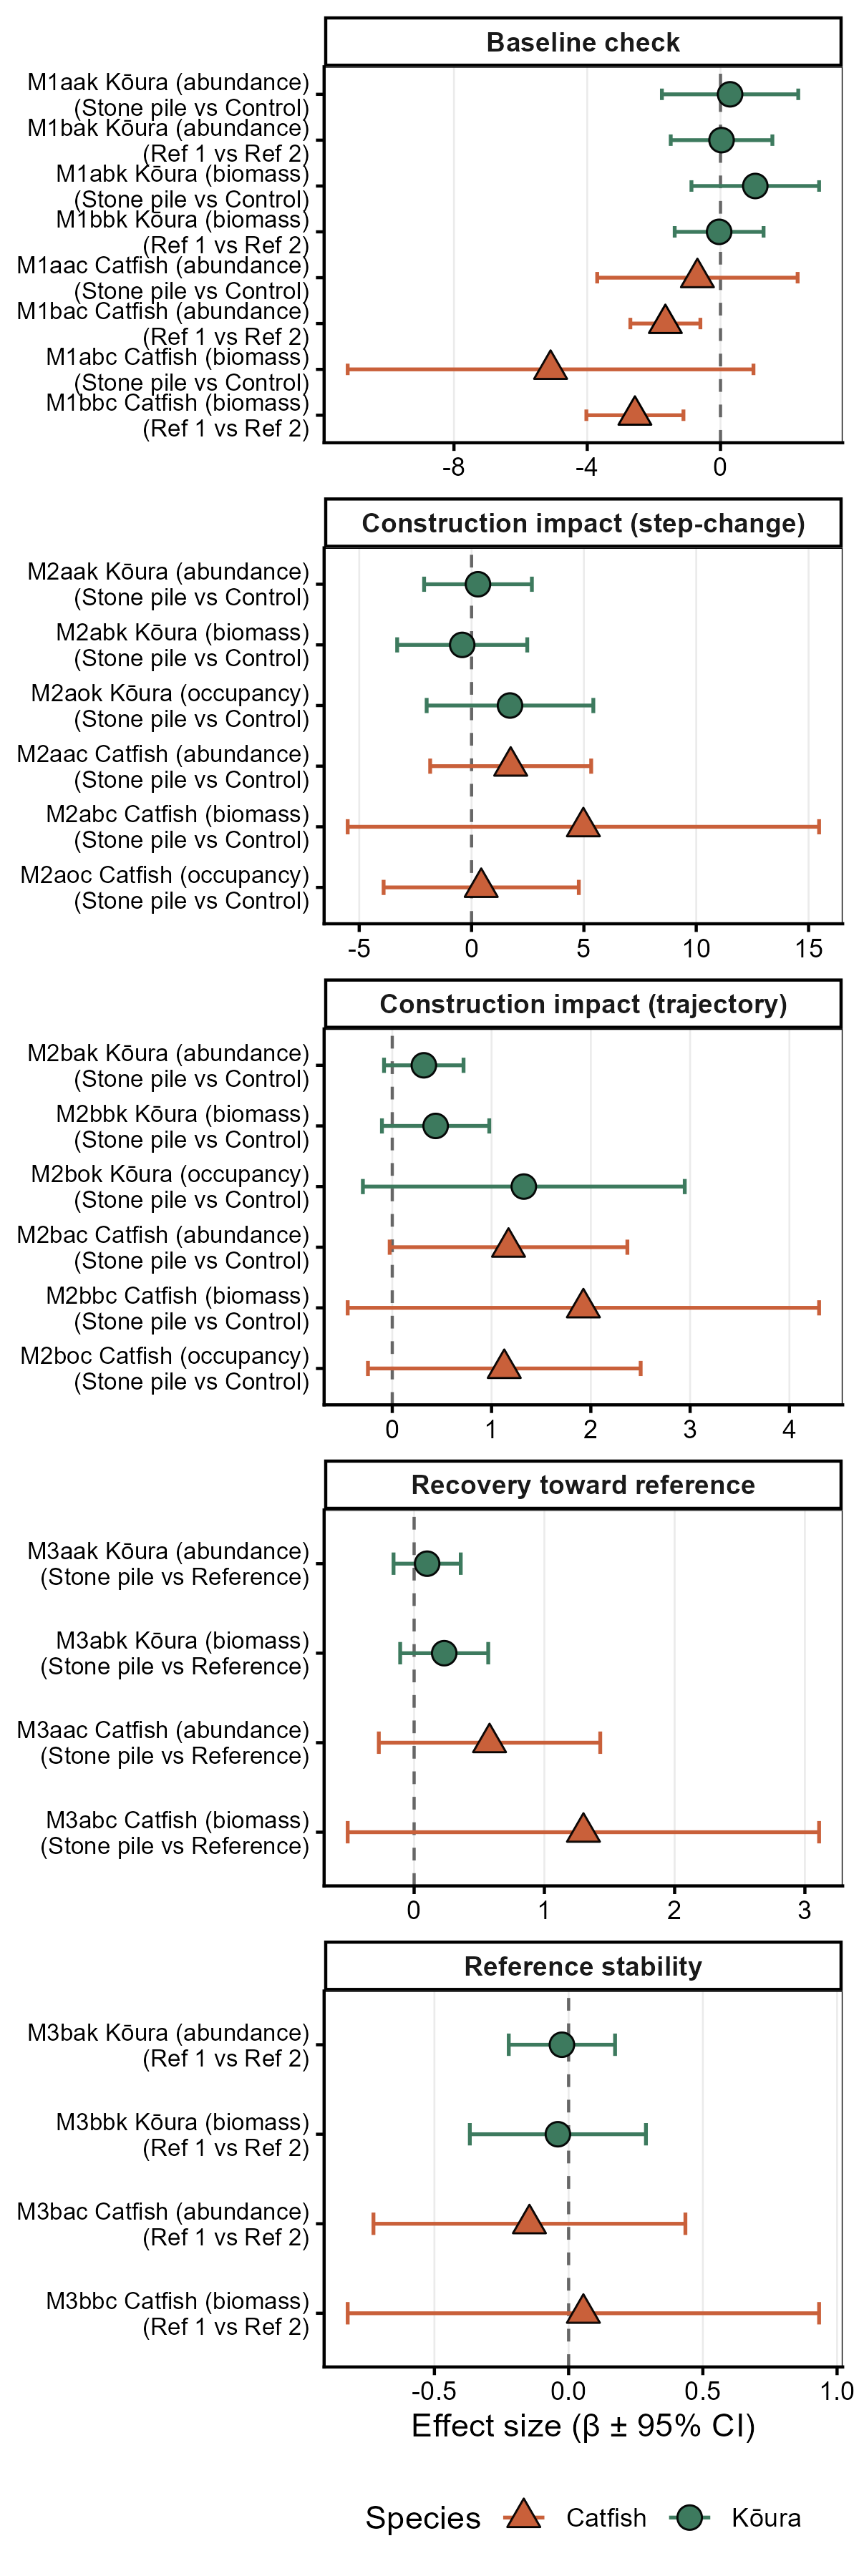
\includegraphics[width=1\linewidth,height=\textheight,keepaspectratio]{outputs/fig-forest-plot.png}

}

\caption{\label{fig-forest-plot}Effect sizes (\(\beta\) ± 95\% CI) for
the key term of interest across all models, separated by species
(columns) and comparison type (rows). Filled points indicate significant
effects (\emph{p} \textless{} 0.05); open points are non-significant.
Each row has its own x-axis scale --- effect magnitudes are not directly
comparable across rows because each comparison tests a different
contrast (step-change, per-round slope, or simple group difference), and
occupancy is on the log-odds scale while abundance and biomass models
use the Tweedie log link. Models with degenerate confidence intervals
are excluded.}

\end{figure}%

\begin{figure}

\centering{

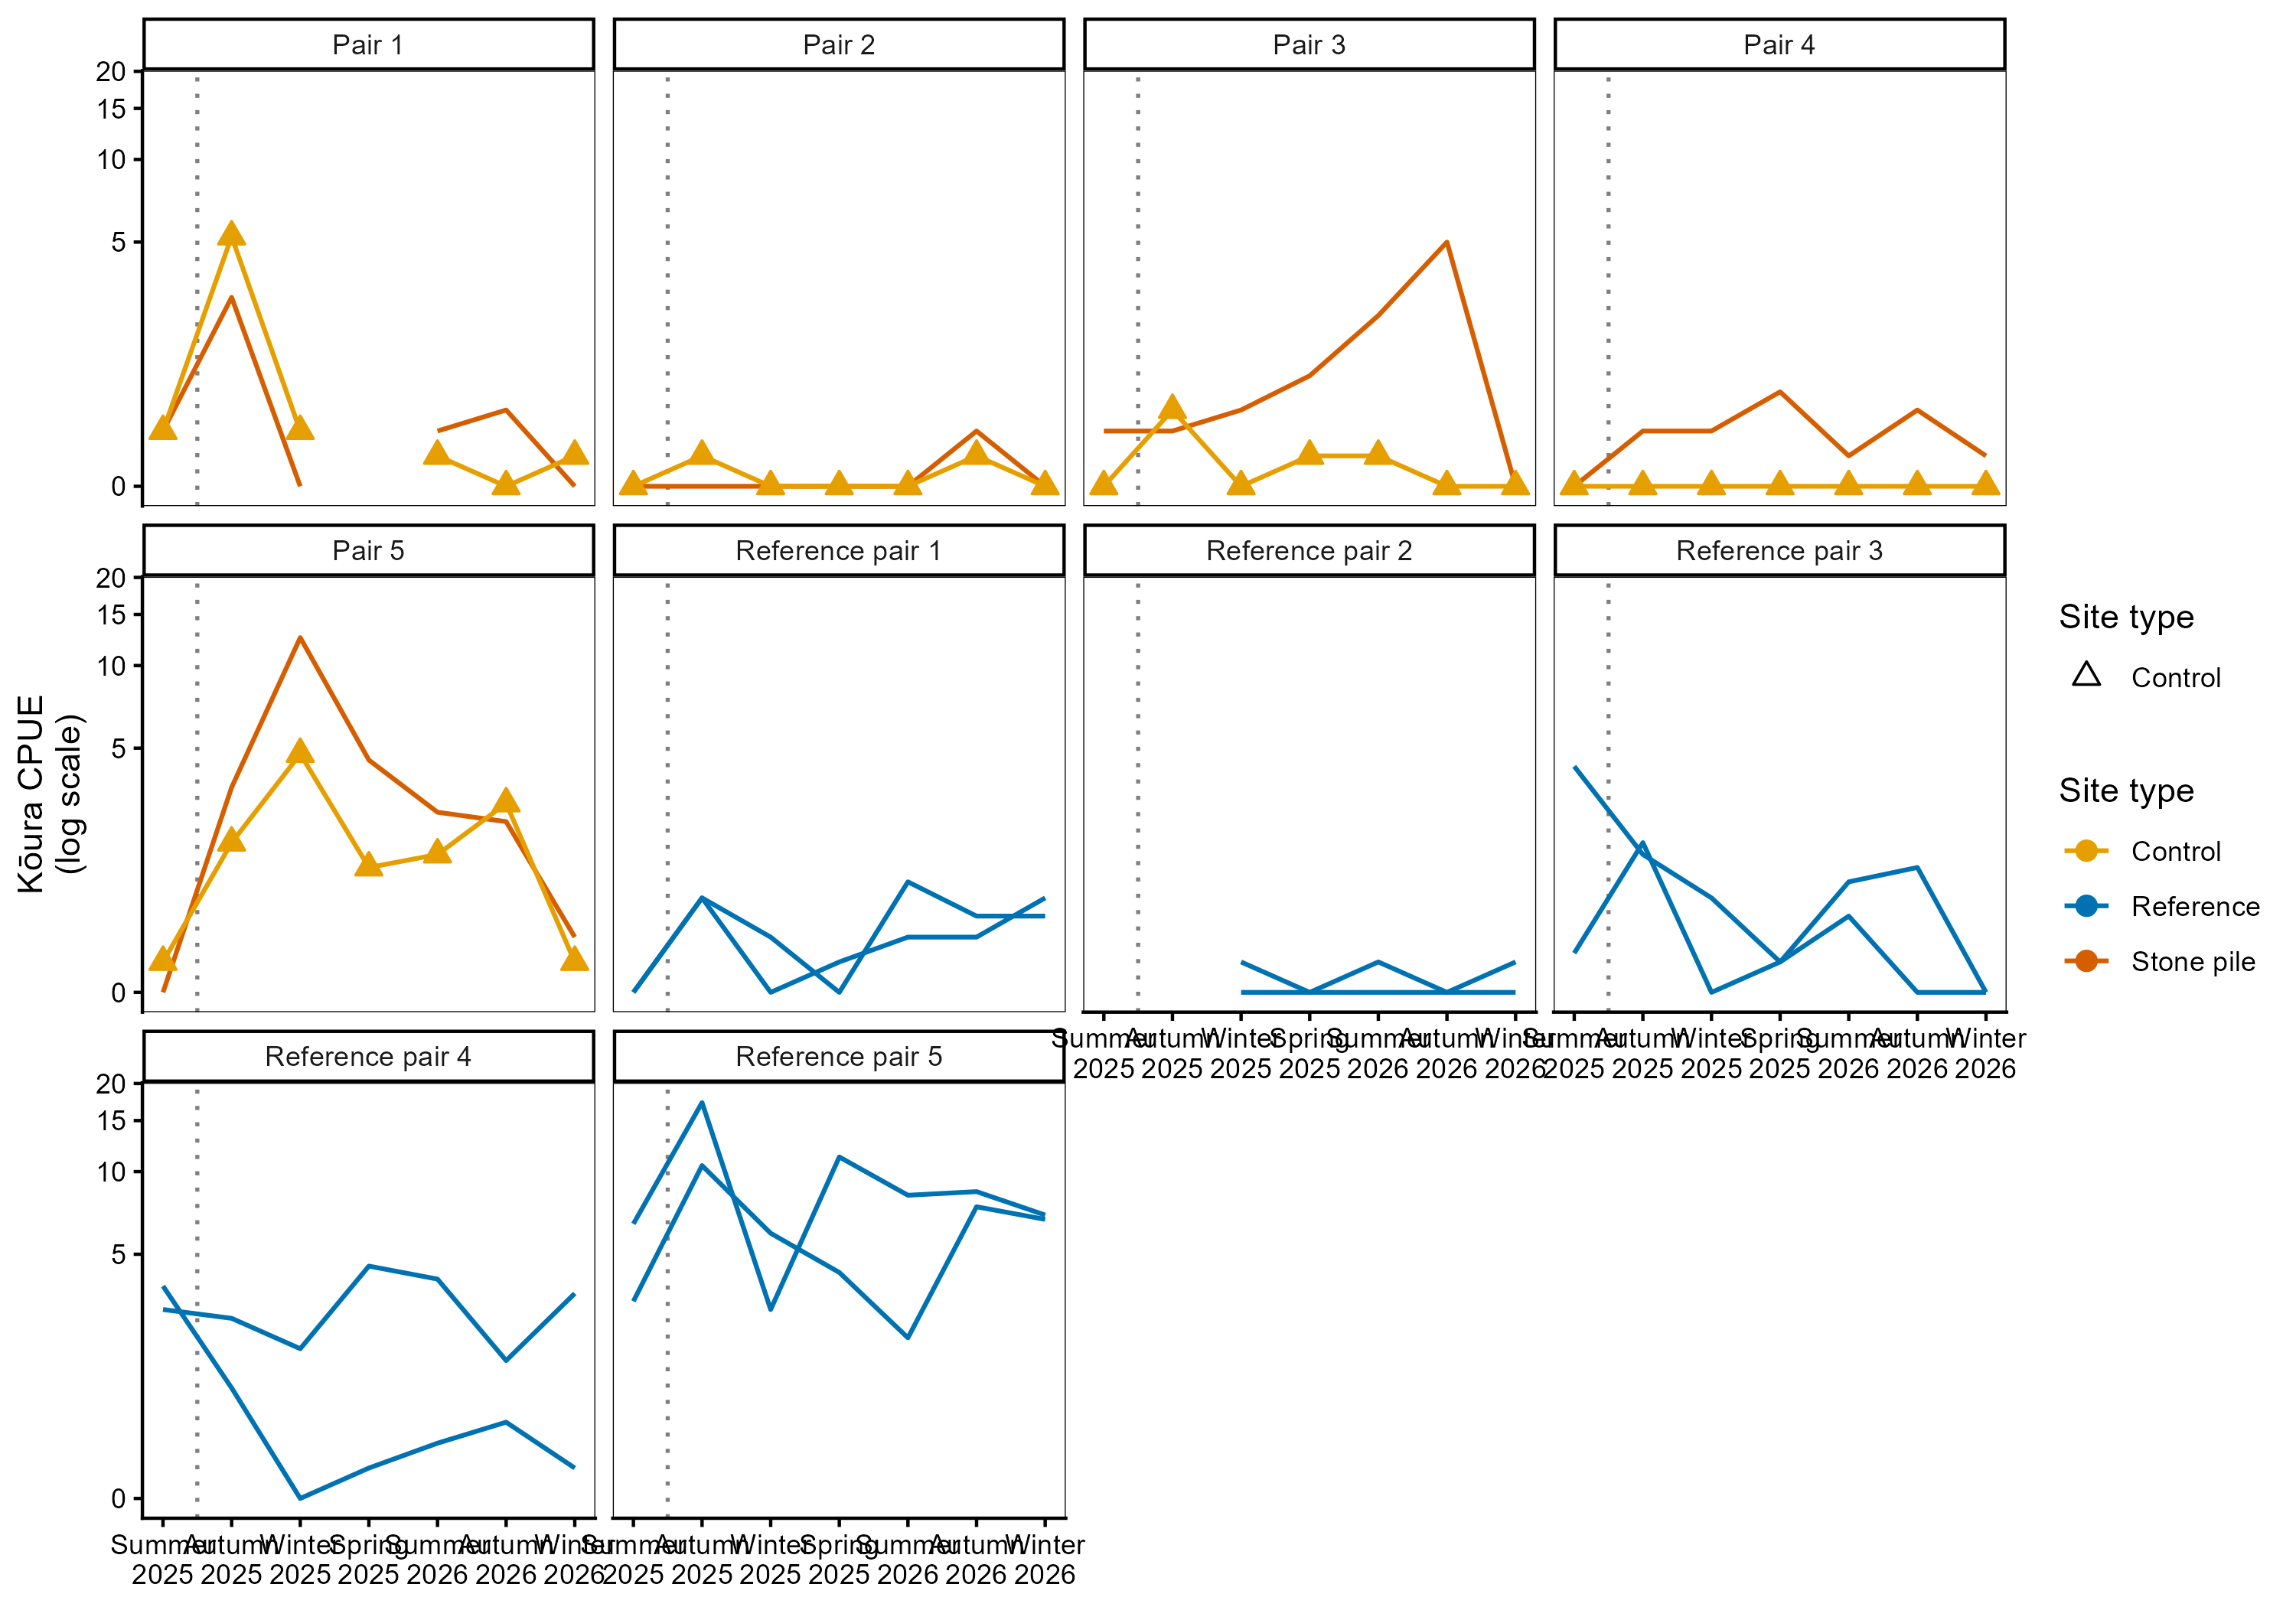
\includegraphics[width=1\linewidth,height=\textheight,keepaspectratio]{outputs/fig-koura-effect.png}

}

\caption{\label{fig-koura-effect}Kōura CPUE at individual site pairs
across all monitoring rounds. Each panel shows one stone pile / control
pair (sites 1--10) or reference pair (sites 11--20). Colour and shape
indicate site type. Vertical dotted line marks stone pile construction.
y-axis on log(1+x) scale.}

\end{figure}%

\begin{figure}

\centering{

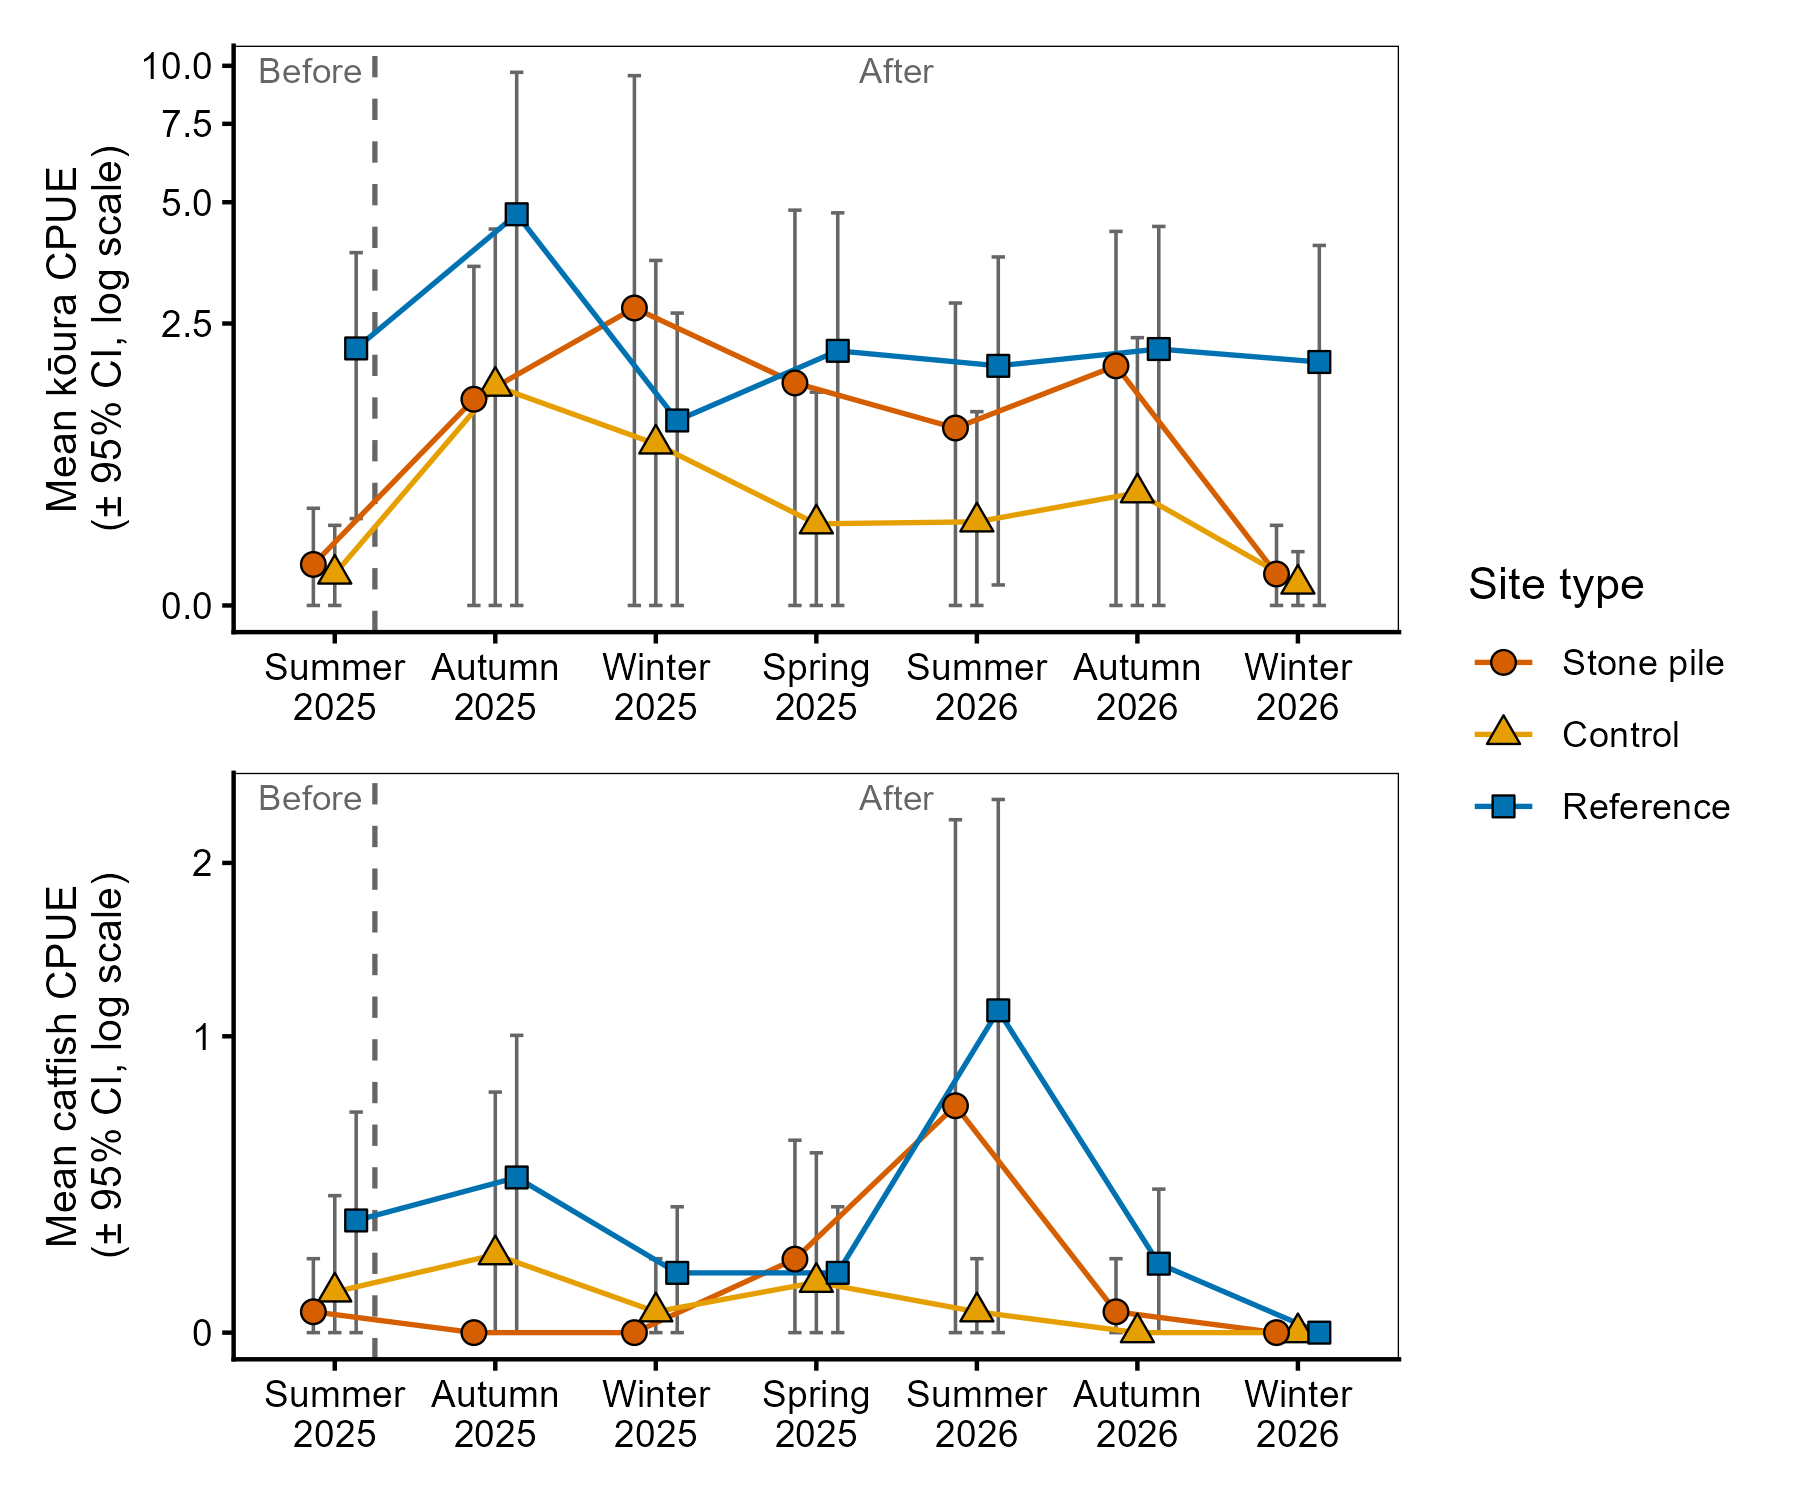
\includegraphics[width=1\linewidth,height=\textheight,keepaspectratio]{outputs/fig-cpue-trends.png}

}

\caption{\label{fig-cpue-trends}Mean CPUE per monitoring round (± 95 \%
CI, log scale) by site type for kōura (top) and catfish (bottom).
Vertical dashed line distinguishes the pre-construction period (Before)
from post-construction monitoring (After).}

\end{figure}%

\begin{figure}

\centering{

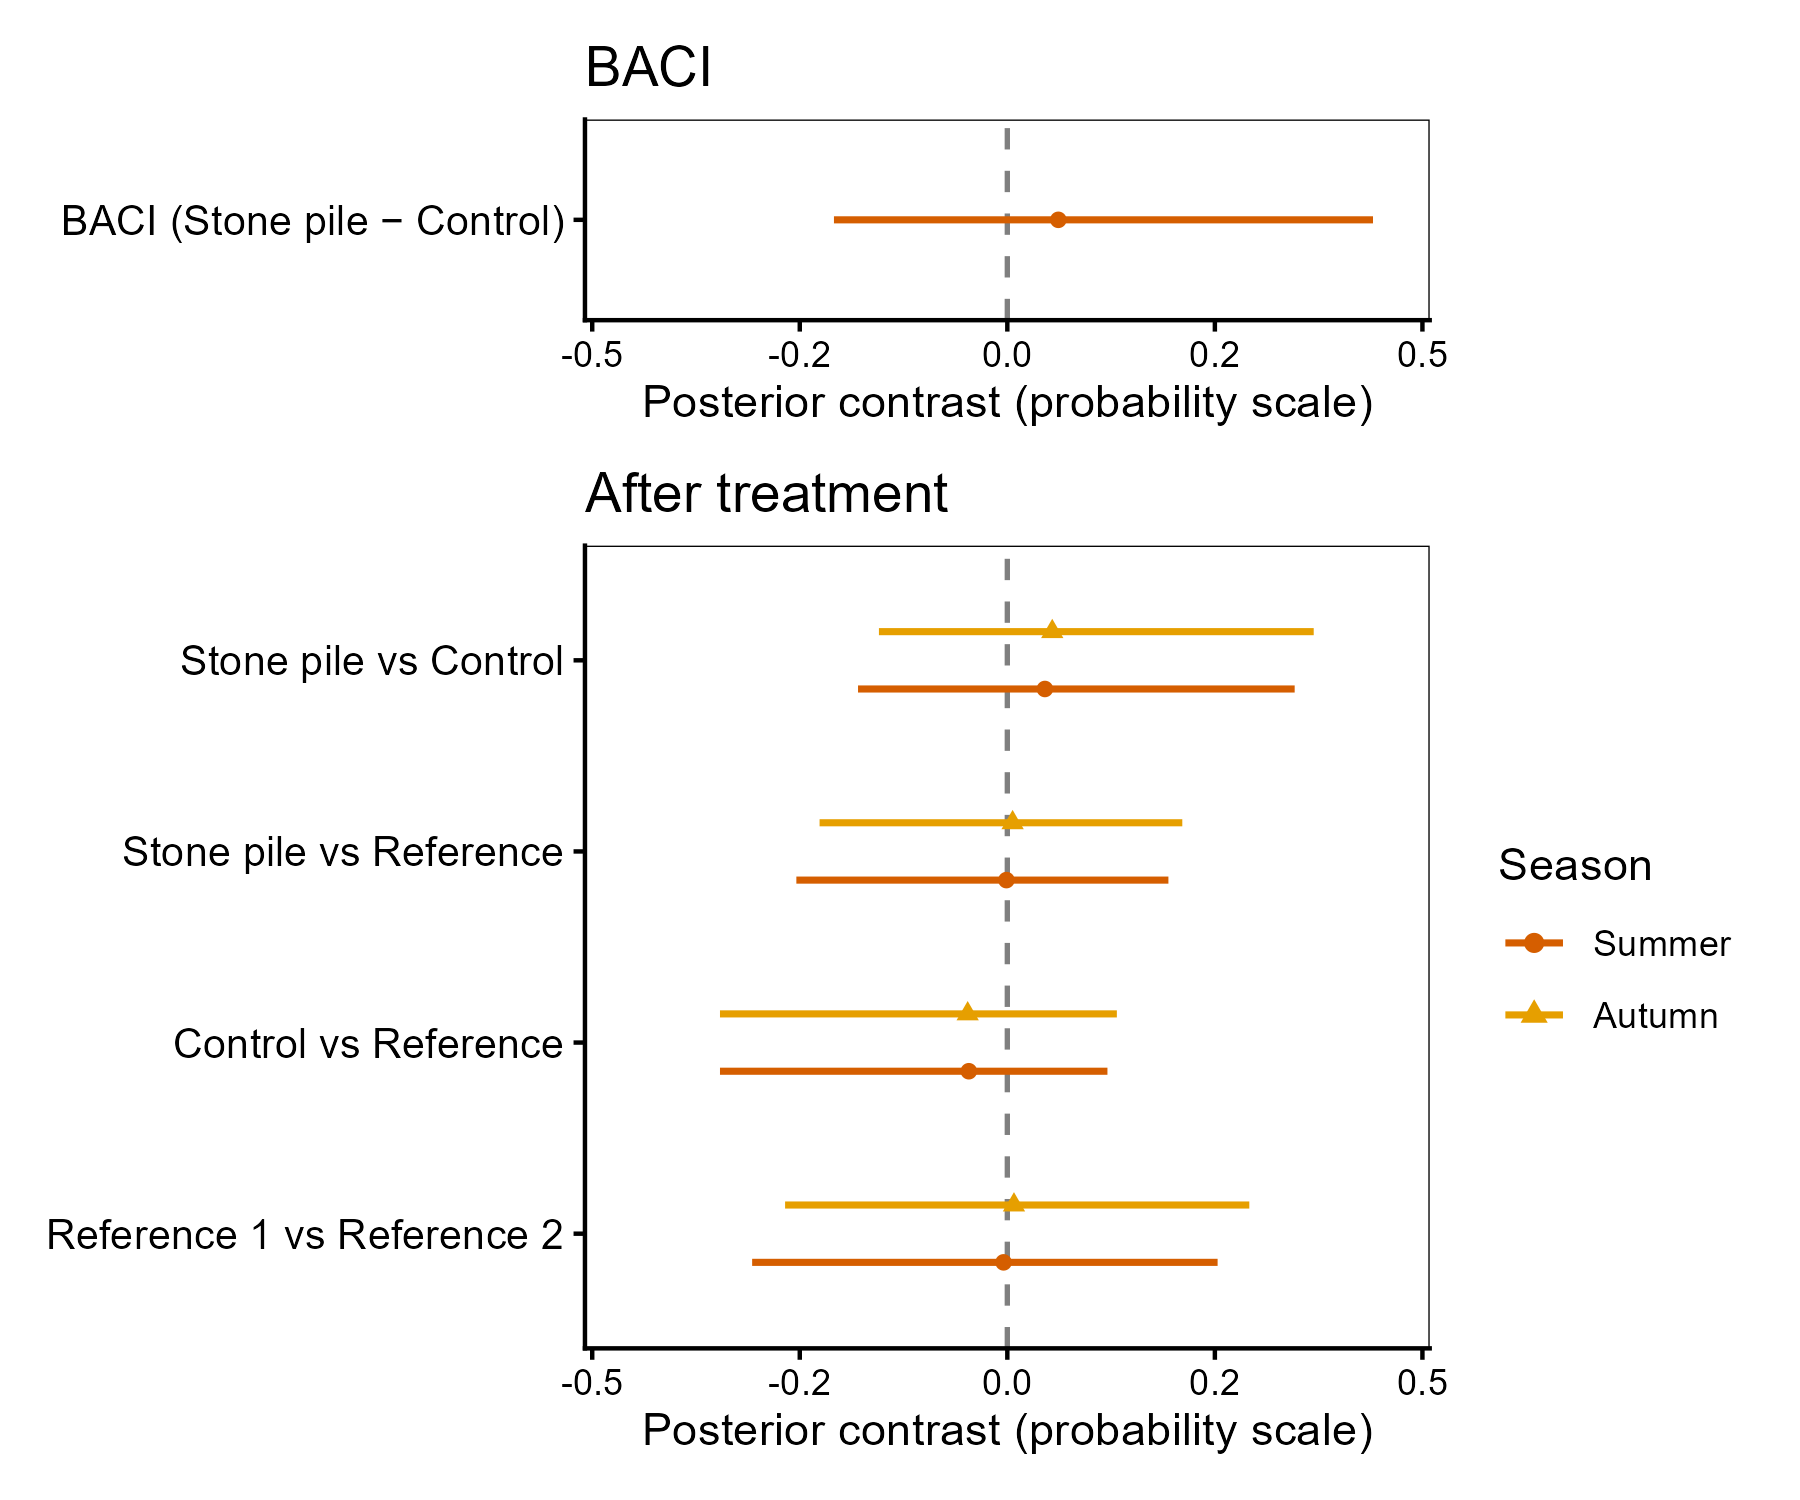
\includegraphics[width=0.8\linewidth,height=\textheight,keepaspectratio]{outputs/fig-occ-warm-contrasts.png}

}

\caption{\label{fig-occ-warm-contrasts}Posterior contrasts in kōura
occupancy from the warm-season model. BACI contrast (stone pile minus
control, before vs after construction). After-treatment contrasts
between all site-type pairs. Points show posterior means with 95 \%
credible intervals; contrasts overlapping zero indicate no detectable
difference.}

\end{figure}%

\begin{figure}

\centering{

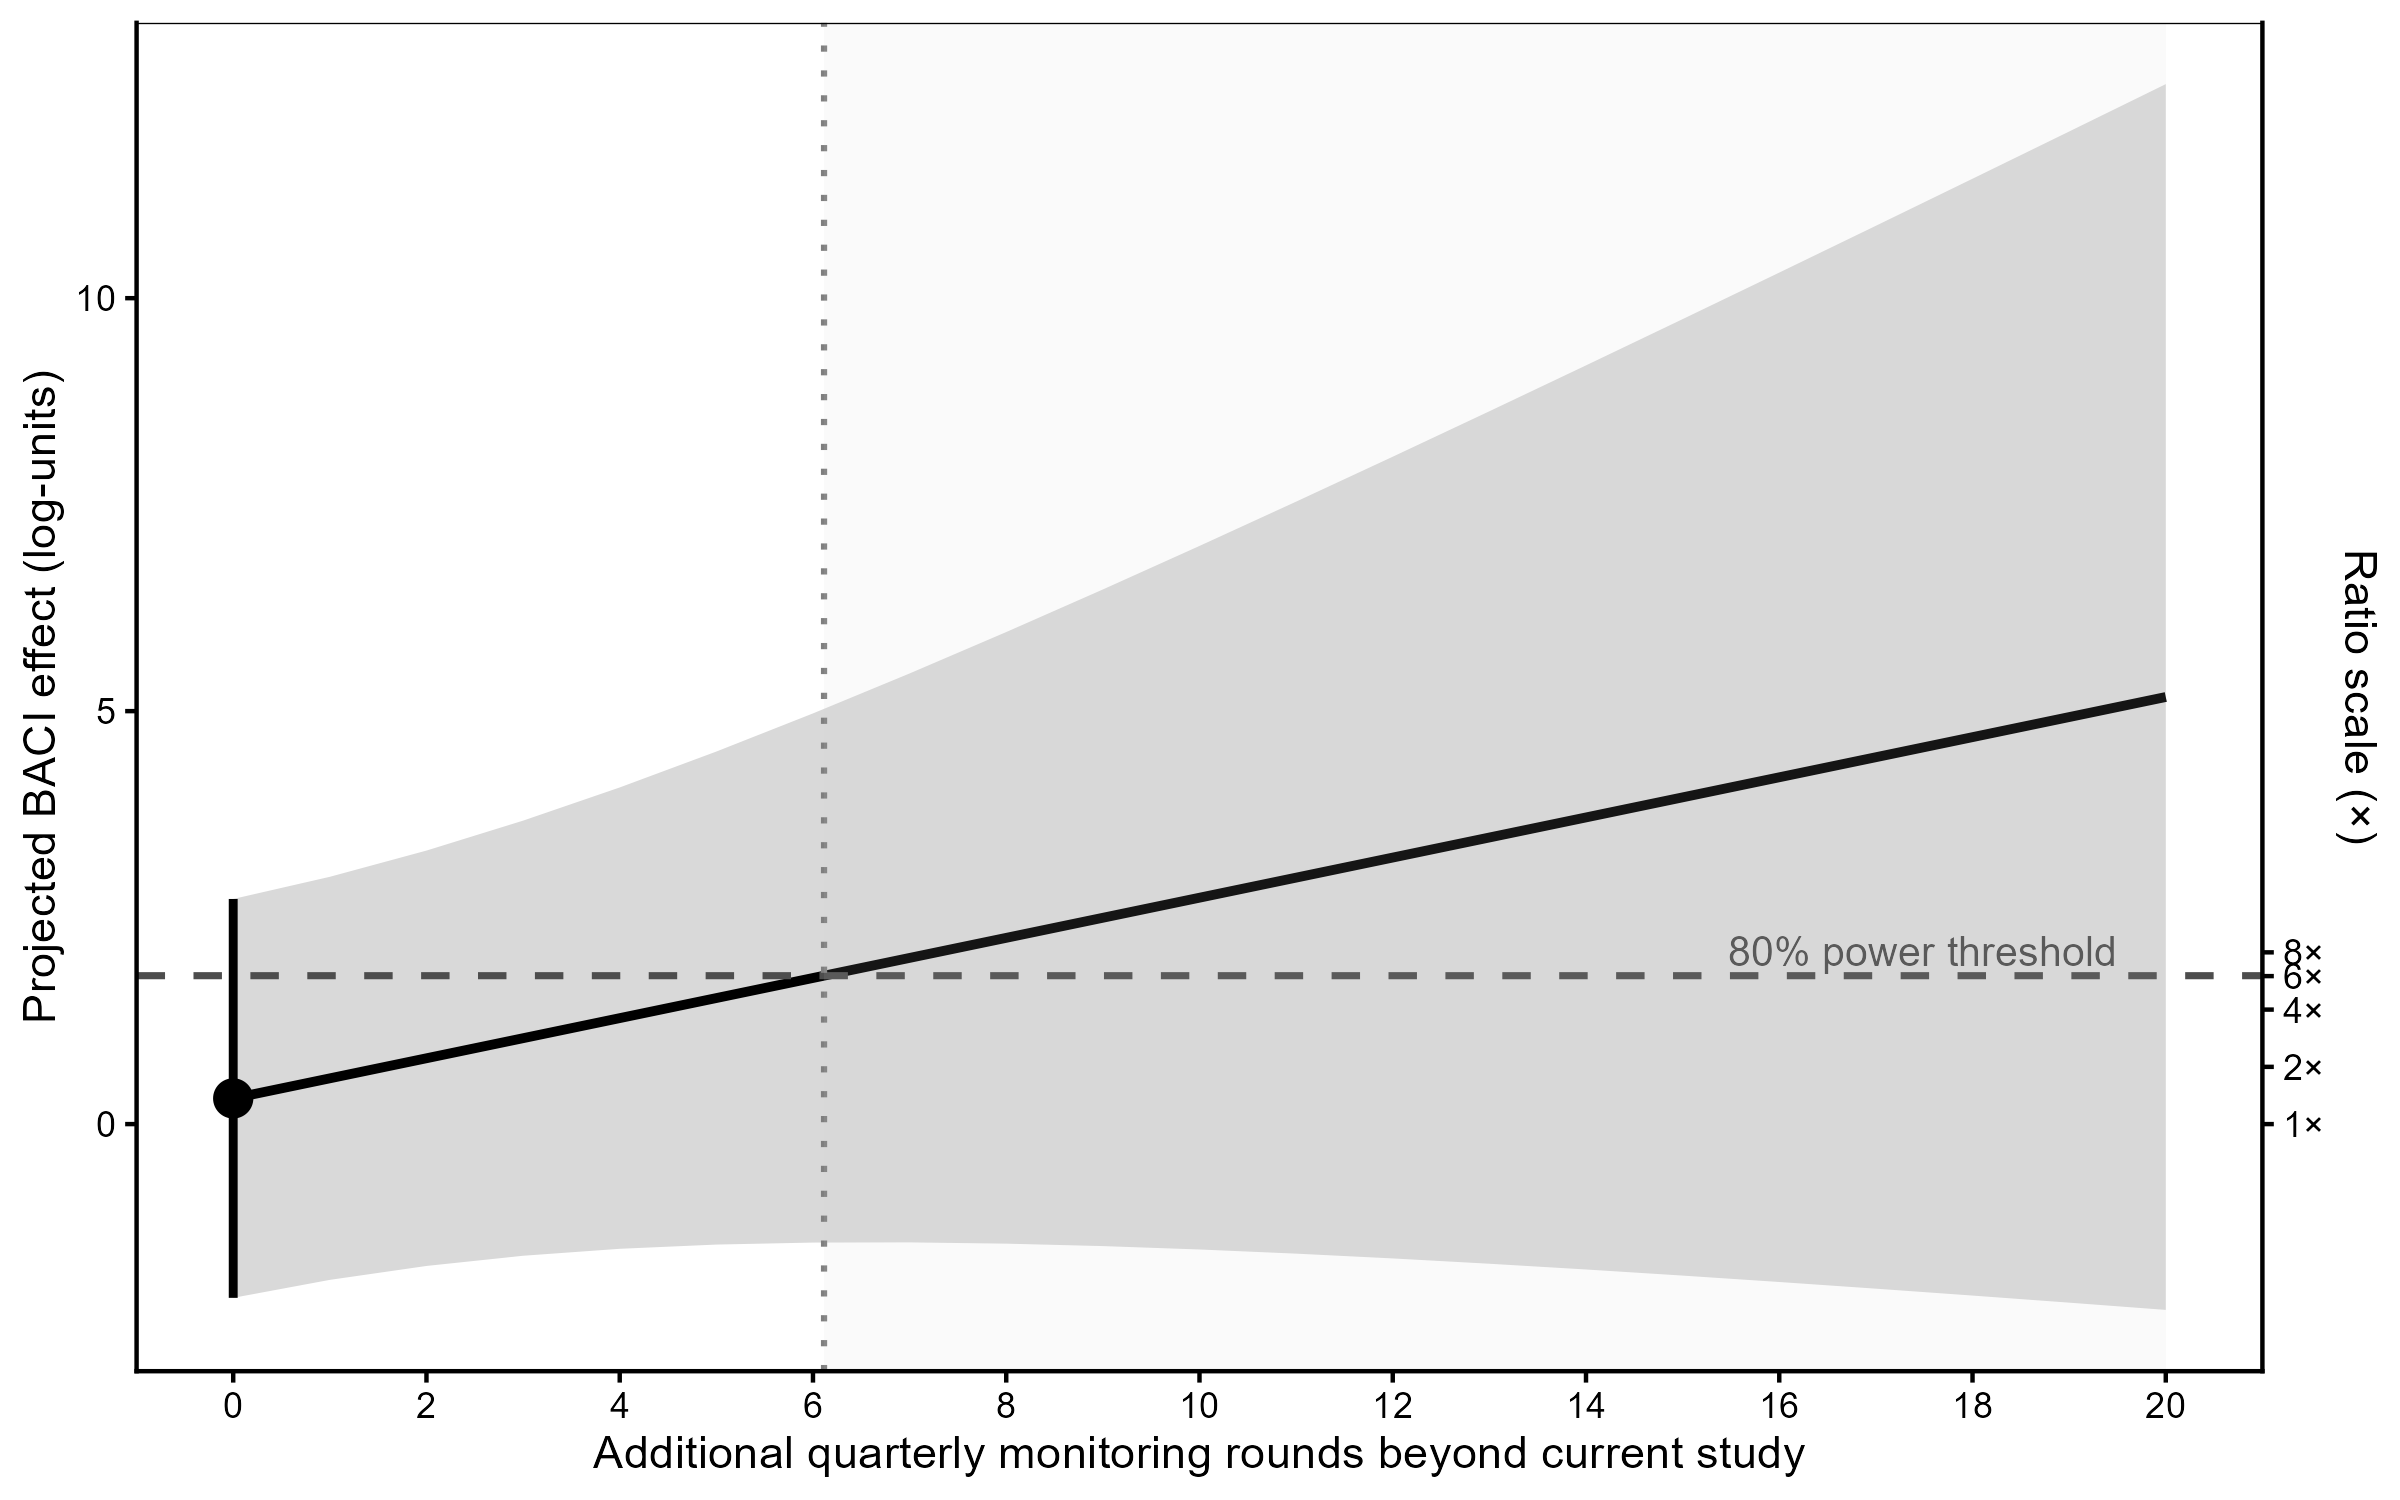
\includegraphics[width=0.8\linewidth,height=\textheight,keepaspectratio]{outputs/fig-trajectory-projection.png}

}

\caption{\label{fig-trajectory-projection}Projected kōura CPUE BACI
effect size over additional monitoring rounds. The solid line shows the
linear projection based on the estimated post-construction trajectory;
shaded ribbon shows 95\% uncertainty interval. Dashed horizontal line
marks the detection threshold for 80 \% power with five site pairs.}

\end{figure}%

\clearpage
\providecommand{\chaptermark}[1]{}
\ifcsname c@chapter\endcsname
\setcounter{chapter}{6}
\setcounter{figure}{0}
\setcounter{table}{0}
\setcounter{section}{0}
\addcontentsline{toc}{chapter}{\protect\numberline{6}Synthesis}
\chaptermark{Synthesis}
\fi
\providecommand{\thechapter}{6}
\thispagestyle{empty}
\begin{tikzpicture}[remember picture, overlay]
  \node[inner sep=0pt] at ([yshift=-1cm]current page.center)
    {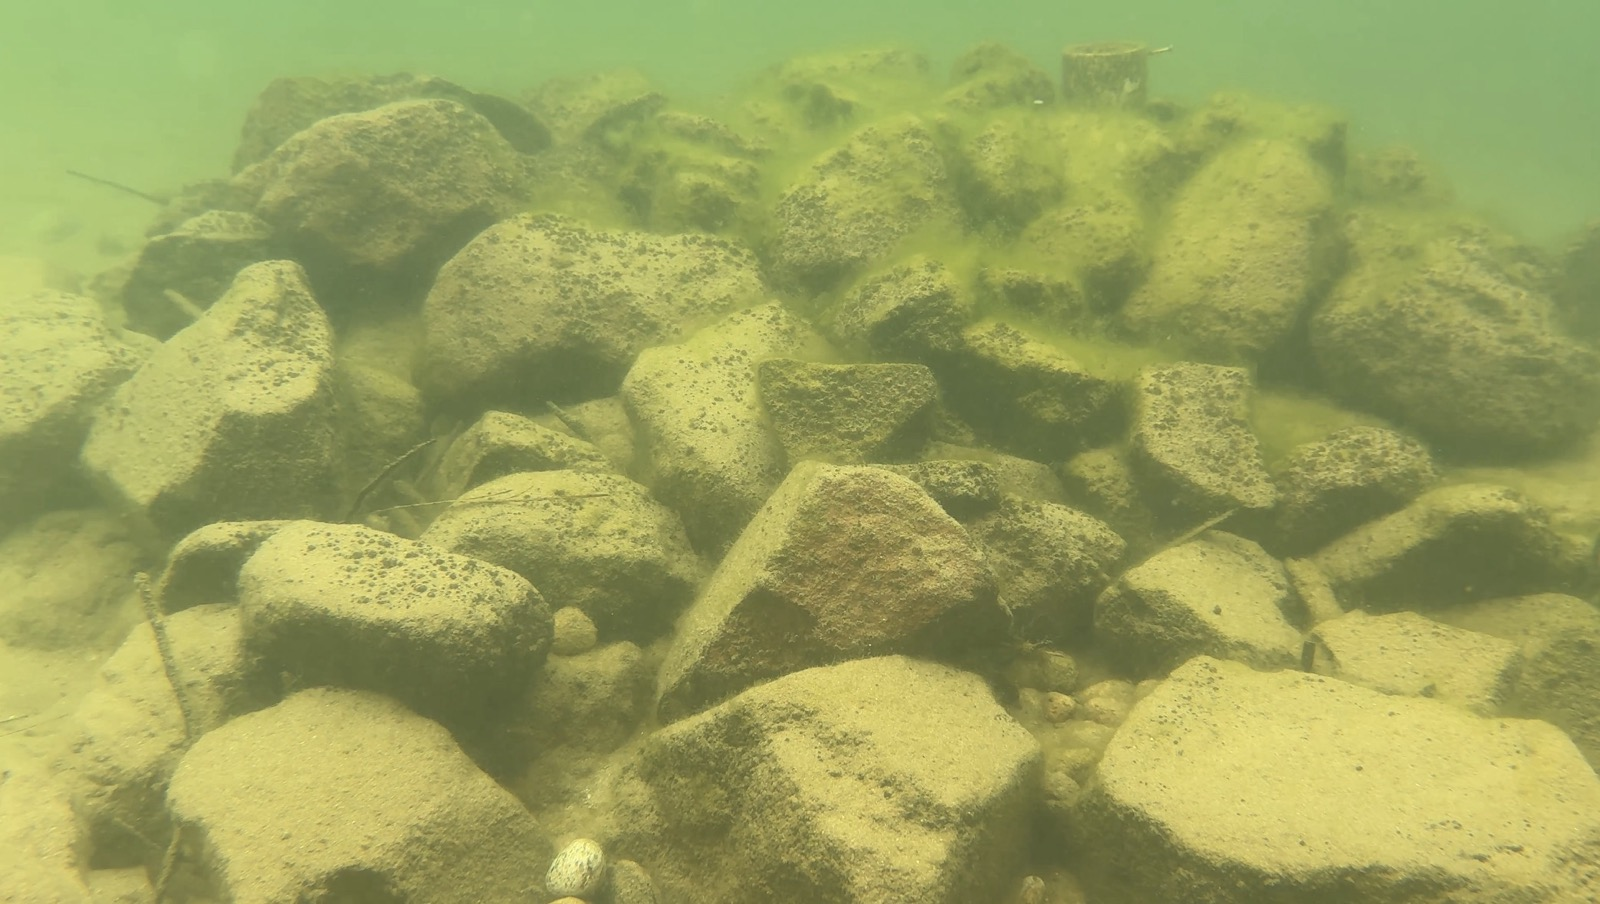
\includegraphics[width=\paperwidth,height=\paperheight]{images/ch6_cover.jpg}};
  \fill[black]
    (current page.north west) rectangle ([yshift=-5.5cm]current page.north east);
  \node[color=thesissand, align=left,
        font=\fontsize{13}{16}\selectfont\sffamily, anchor=west]
    at ([xshift=1.5cm, yshift=-1.3cm]current page.north west)
    {Chapter \thechapter};
  \node[color=white, text width=0.85\paperwidth, align=left,
        font=\fontsize{22}{28}\selectfont\bfseries\sffamily, anchor=west]
    at ([xshift=1.5cm, yshift=-3.5cm]current page.north west)
    {Synthesis};
\end{tikzpicture}
\null
\clearpage

\section{Introduction}\label{introduction-4}

The chapters preceding this synthesis established the ecological and
practical basis for using stone piles as a kōura habitat enhancement
tool. Behavioural experiments (Chapter 2) confirmed that kōura respond
with heightened refuge use to novel predators than native ones. Field
observations (Chapter 3) identified the habitat features that support
kōura along lake shorelines, and mesocosm trials (Chapter 4) showed that
structure stability and complexity matter more than material when kōura
select shelter. Chapter 5 deployed stone piles along the shoreline of
Lake Rotoiti and monitored kōura response over 18 months in a BACI
design. Kōura colonised the structures rapidly, with occupancy and
abundance consistently trending positive at stone pile sites relative to
controls, though this effect did not reach statistical significance.
Catfish showed no evidence of being attracted to the stone piles. This
chapter (Chapter 6) synthesises the findings across all four chapters
and presents two pilot studies that extend the work in early and future
directions. The first trialled the construction logistics and kōura
reintroduction in Lake Ōkaro where it was found that water quality needs
to meet kōura demands before reintroduction is feasible. The second
extended stone pile deployment up to nine meters deep and found that
kōura use stone piles across the littoral zone and that stone piles are
able to suppress invasive macrophytes. Together with the main chapters,
these case studies broaden the application of the kōura restoration
approach developed in this thesis for future deployment and monitoring.

\section{Three stressors working
together}\label{three-stressors-working-together}

Kōura decline in the Rotorua Te Arawa Lakes is driven by multiple
compounding stressors, most prominently catfish predation, thermal
stratification, and invasive macrophytes, which togeheter operate at
both the local habitat scale and the broader lake scale.

Chapter 2 supported the generalised fear hypothesis: koura resond with
heightened refuge use to catfish compared to the native eel, meaning
fear-induced behavioural suppression operates even in the absence of
direct predation. An animal spending more time in refuge is an animal
spending less time foraging, leading to slower growth and reduced
reproductive output. This is the core mechanism behind the landscape of
fear (Laundré et al. 2001), where predators do not need to eat every
prey individual to suppress a population, but their presence alone is
sufficient to reshape how prey use space and time, and those behavioural
changes carry demographic consequences. In the context of the Rotorua Te
Arawa Lakes, this means that catfish suppress kōura populations through
two channels simultaneously. Direct predation removes individuals and
fear-induced behavioural change reduces the reproductive capacity of
those that survive. Population recovery under these conditions is likely
to be slow even if predation rates are reduced, because the behaviour
suppression persists as long as catfish are present.

Chapter 3 showed a comparison between five lakes, where oligotrophic
lakes with no catfish had the highest overall kōura catches, while
eutrophic lakes with catfish, and anoxic stratification yielded
substantially lower kōura numbers. On the habitat scale structurally
complex rocky shorelines were associated with more kōura abundance while
excessive macrophyte cover revealed lower kōura densities, confirming
that some stressors operate at lake scale while others matter at the
habitat scale.

Habitat enhancement represents an important intervention under these
conditions. The mesocosm trials (Chapter 4) showed that kōura
preferentially select stable, crevice-rich structures, exactly the
properties that stone piles provide in the field, suggesting that the
positive trend in Chapter 5 reflects genuine preference rather than
incidental use. Chapter 5 showed that stone piles in Lake Rotoiti
attracted kōura densities approaching those on natural rocky substrates,
despite the ongoing presence of catfish. High-quality refuge does not
eliminate the fear response, but it provides kōura with locations where
they can shelter effectively, emerge to forage in relative safety, and
maintain sufficient activity levels to reproduce. In catfish-invaded
lakes where predator eradication is ongoing, habitat provision may
therefore be what allows a remnant population to persist and slowly
recover rather than declining to local extinction. Stone piles are not
solving fear responses but they could be helpful in managing its
consequences.

Kōura use of stone pile refuges in the littoral zone was strongly
seasonal (Chapter 5), as during summer and autumn when stratification
and catfish shoreline use simultaneously peaks, kōura are compressed in
this small zone full of danger. Until winter comes, stratification
breaks down and kōura can redistribute to deeper habitats. Climate
projections suggest this dynamic will intensify as surface waters get
warmer, stratification strengthens, and anoxic events become more
frequent and prolonged, making conditions more favourable for catfish
({Jane et al.} 2021; Woolway et al. 2021; Lee et al. 2025). Chapter 1
documents the decline in liveable habitat for kōura over the last 20
years across eleven of the lakes, with for example, a statistically
significant annual trend of −0.4\%/yr in Lake Ōkāreka, confirming that
the thermal compression window is narrowing under current conditions,
not just future ones.

\section{Case study - field trial stones piles Lake
Ōkaro}\label{case-study---field-trial-stones-piles-lake-ux14dkaro}

A trial in Lake Ōkaro tested stone pile construction logistics and kōura
reintroduction feasibility, revealing that habitat enhancement alone
cannot support population recovery when water quality remains below
kōura tolerance thresholds. Lake Ōkaro is one of the smaller Rotorua Te
Arawa volcanic lakes with an area of 30 ha, a max depth of 18 m and a
mean depth of 12 m. Water quality in the lake has been very poor with
trophic state flipping between hypereutrophic and eutrophic and frequent
algal blooms (Paul et al. 2008; LAWA 2024). To improve water quality in
the lake, in 2007 a wetland has been constructed to remove nitrogen and
sediments from the main inflows into the lake (Hudson et al. 2009) and
alum dosings (aluminium sulfate) are carried out as in lake phosphorous
treatment (Paul et al. 2008). Kōura have not been observed in Lake Ōkaro
in monitoring surveys from 1981 to 2007 (Parkyn and Kusabs 2007) and
monitoring in 2016 and 2017 still were not able to observe kōura in the
lake even as water quality had improved (Kusabs 2017). Water quality has
now improved sufficiently that kōura is considered feasible but natural
recolonisation has not happened yet, therefore reintroduction might be
possible. Lake Ōkaro is stocked with trout for angling and as a predator
of kōura, stone piles would provide additional refuge to trial habitat
enhancement alongside the existing trout stocking. The lake has no stone
or rocky substrates therefore the construction of two stone piles would
provide initial refuge for the introduced kōura in the lake.

Stone pile construction was carried out collaboratively with Te Arawa
Lakes Trust, Tūhourangi, Ngāti Tahu-Ngāti Whaoa, Te Mana o Ngāti
Rangitihi Trust, and Bay of Plenty Regional Council. Two stone piles
(each 5 m × 2 m, depth 1 m; stones 70--210 mm, mean 120 mm; total 5
m\(^{3}\)) were placed 3 and 6 m from the northeast shore, with stones
sourced from local Rainbow Quarry on Rainbow Mountain. Dissolved oxygen
and temperature were monitored using three HOBO U26-001 loggers (± 0.2
mg/L DO, ± 0.2 °C; Onset Computer Corporation, Bourne, MA, USA), with
two loggers buried within the stone piles and one at the control site,
over six months from September 2024. Prior to kōura release, trapping
and spotlighting surveys confirmed the lake held no kōura. In October
2024, twenty kōura sourced from Lake Rerewhakaaitu were released onto
the stone piles to initiate recolonisation.

In the early summer of 2024 the lake stratified rapidly with oxygen
levels dropping quickly and at December 10th oxygen levels reached less
than 3 mg/L at surface level for multiple days
(Figure~\ref{fig-okaro-combined}). The HOBO loggers in the stone piles
and the control next to the structures showed that inside the structures
the dissolved oxygen levels dropped slightly faster than compared to the
control site, and that the daily average of dissolved oxygen was lower
than outside of the stone piles (Figure~\ref{fig-okaro-combined}). This
is expected as the sensors inside the stone pile received less water
mixing and were in close proximity to periphyton, which draws down
dissolved oxygen through respiration during the night. During anoxic
events, kōura are expected to move to the outer margins of the stone
piles or emerge entirely, as DO levels inside the structure would fall
below tolerance. Despite this anoxic event one kōura was repeatedly
observed at the stone piles from January 2025 till June 2025 (pers.
comm. Ian Kusabs). Expected is that the other kōura have spread out
through the lake. The last spotlight session (July 2026) found no kōura,
but revealed that the previous sandy shoreline around the stone piles
had been colonised by milfoil (\emph{Myriophyllum propinquum}) (pers.
comm. Ian Kusabs).

\begin{figure}

\centering{

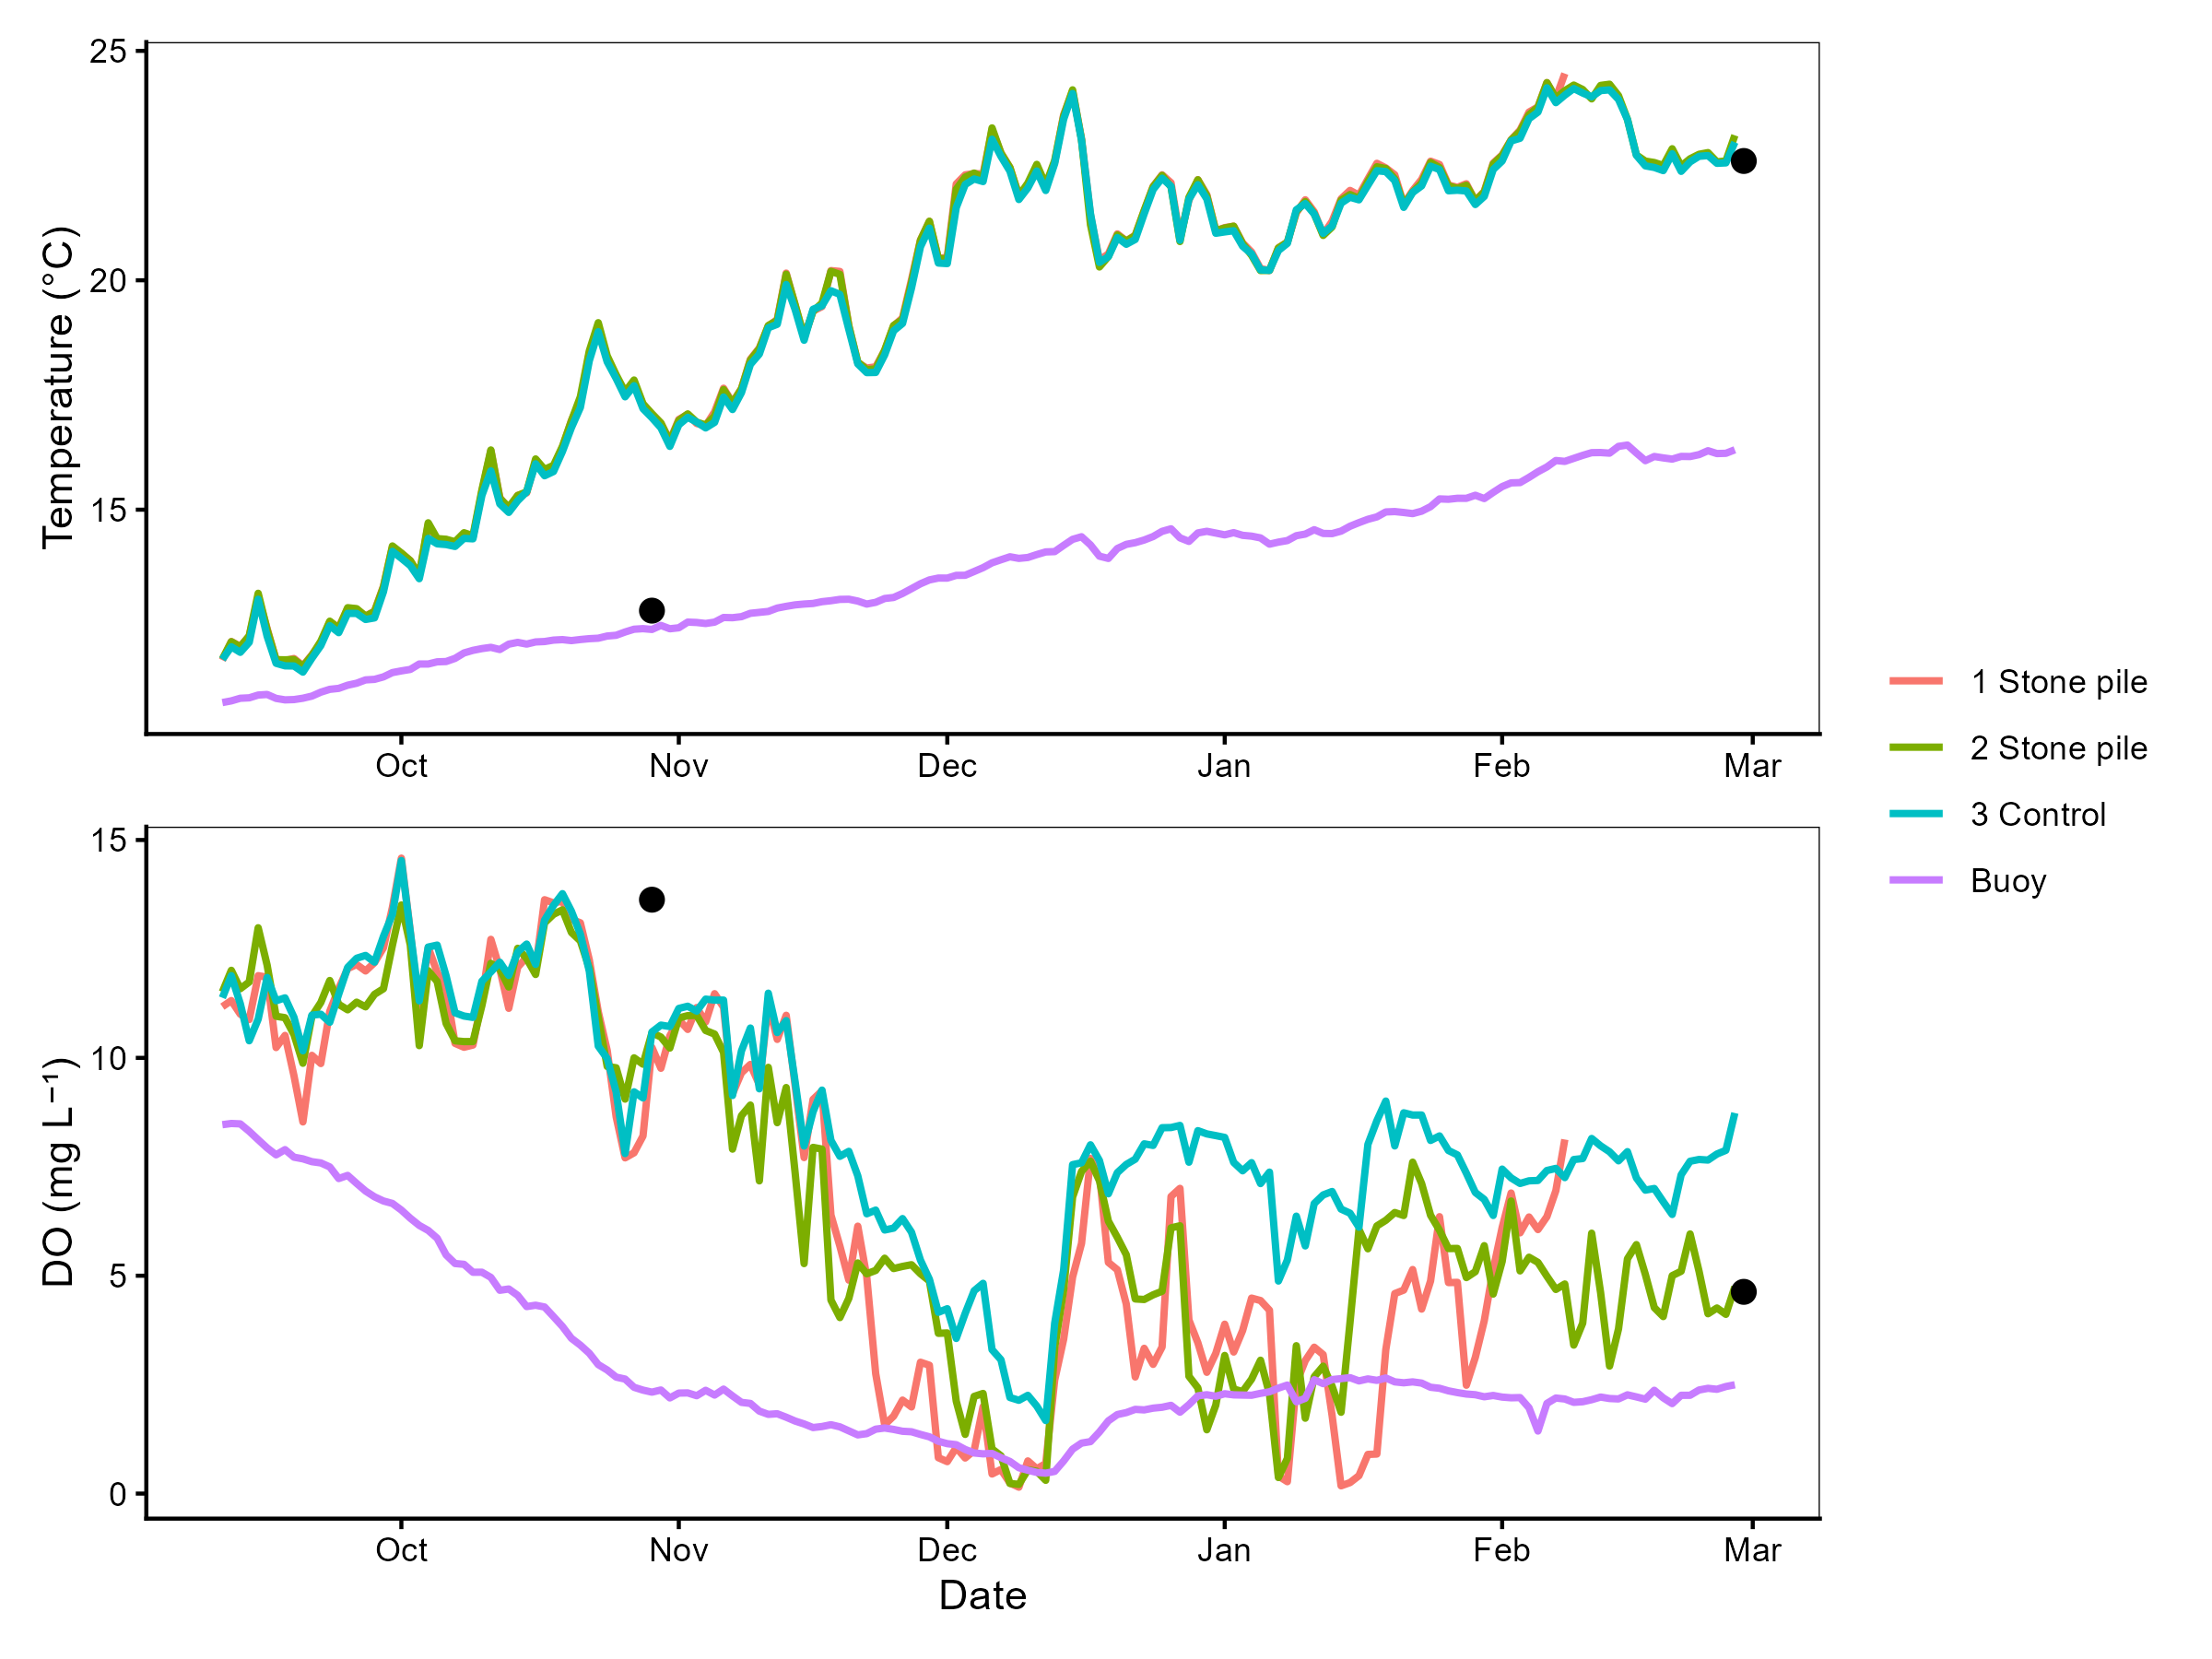
\includegraphics[width=0.8\linewidth,height=\textheight,keepaspectratio]{outputs/fig-okaro-combined.png}

}

\caption{\label{fig-okaro-combined}Daily mean water temperature (top)
and dissolved oxygen (bottom) at Ōkaro stone pile, control sites, and
the lake monitoring buoy \textless{} 1m. Period: 2024-09-11 to
2025-02-27. Buoy data derived from CTD cast collected by LimnoTrack
(Moore2026).}

\end{figure}%

Construction by hand proved to be a simple and low-cost method for
building shallow shorelines structures. The smaller stone size used in
Ōkaro (range 70-210 mm; mean 120 mm) required more handling effort and
provided limited crevice space for larger kōura. For the Rotoiti
deployment, slightly larger stones (85-315 mm; mean 173 mm) were
selected, a size that could be thrown from the trailer edge directly
into the lake and repositioned by hand if needed.

The Ōkaro trial demonstrated that habitat enhancement cannot succeed
ahead of water quality recovery. The anoxic event that followed stone
pile deployment confirmed that structural complexity provides no benefit
when dissolved oxygen drops below kōura tolerance, kōura cannot use a
refuge they cannot survive in.

\section{Case study - deep stone piles Lake
Rotoiti}\label{case-study---deep-stone-piles-lake-rotoiti}

Extending stone pile deployment across a depth gradient in Lake Rotoiti
showed that kōura use structures beyond the shallow littoral zone and
that stone coverage suppresses invasive macrophyte growth, providing
additional insights to the findings of Chapter 5. Stone piles deployed
in the preceding chapters, and in the Ōkaro trial, were built by hand
from the shore and therefore limited to shallow, nearshore depths.
Extending deployment across a depth gradient required working from a
boat, which opened two additional possibilities: placing structures at
depths beyond wading distance, and positioning them within invasive
macrophyte beds to test whether stone coverage could suppress growth.
Monitoring at greater depths is not well suited to standard netting, so
spotlighting, remotely operated vehicle (ROV) surveys, and human diving
were used before and after construction at this deep Lake Rotoiti site.
Spotlighting was executed after sunset along the shoreline and the area
around the jetty, by observing for kōura using a torch. Each kōura was
counted and their size estimated. The stone piles in the macrophyte bed
and deeper were monitored using a FIFISH V-EVO (4K 60 fps camera; 166°
field of view; QYSEA Technology, Shenzhen, China). The ROV was used to
swim transects at the location of the stone piles and kōura observed
were counted. Spotlight and ROV monitoring was executed two times before
stone pile construction, and day-time diving was executed once before
construction.

Four stone piles were constructed in November 2025 using a boat and
winch system. Three stone piles were positioned perpendicular to shore,
beneath a jetty (\textasciitilde1 m), within an invasive macrophyte bed
(\textasciitilde4 m), and at the macrophyte edge (\textasciitilde8 m),
with wooden slabs placed first to prevent sinking into the sandy
sediment. A fourth pile was placed on bedrock 120 m away.

Pre-construction surveys detected low kōura numbers at the site, two by
spotlighting and two by ROV in June 2025 (water temp 13 °C), and zero by
spotlighting but seven by ROV in August 2025 (water temp 11 °C). Daytime
diving in November 2025 (water temp 19 °C), before construction, found
no kōura. Following construction kōura numbers increased noticeably. The
May 2026 survey (water temp 16 °C) found seven kōura by spotlighting
around the jetty and eleven on the deeper stone pile by ROV. The August
2026 survey (water temp 10 °C) found six by spotlighting and two by ROV,
one on the stone pile in the macrophyte bed and one at the deeper stone
pile. Most kōura were observed at the margins of the stone piles rather
than within them, as internal crevices were visually inaccessible to
both spotlighting and ROV surveys. Kōura were only detected when they
emerged to forage, and ROV footage confirmed they did so despite
thruster noise. The stone pile placed within the macrophyte bed showed
complete suppression of macrophyte growth, though dense macrophyte
growth at the margins complicated kōura detection in that area. Daytime
diving surveys (January 2026, water temp 21 °C; July 2026, water temp 11
°C) detected no kōura on either occasion. As kōura are nocturnal,
daytime diving surveys were expected to yield lower counts as kōura are
likely sheltering within the structures. Dissolved oxygen, measured with
HOBO U26-001 loggers at the stone piles, remained above the 5 mg/L kōura
tolerance threshold throughout the monitoring period, confirming that
the stone piles maintained habitable conditions, in contrast to the
anoxic conditions that compromised the Ōkaro deployment
(Figure~\ref{fig-deep-combined}).

\begin{figure}

\centering{

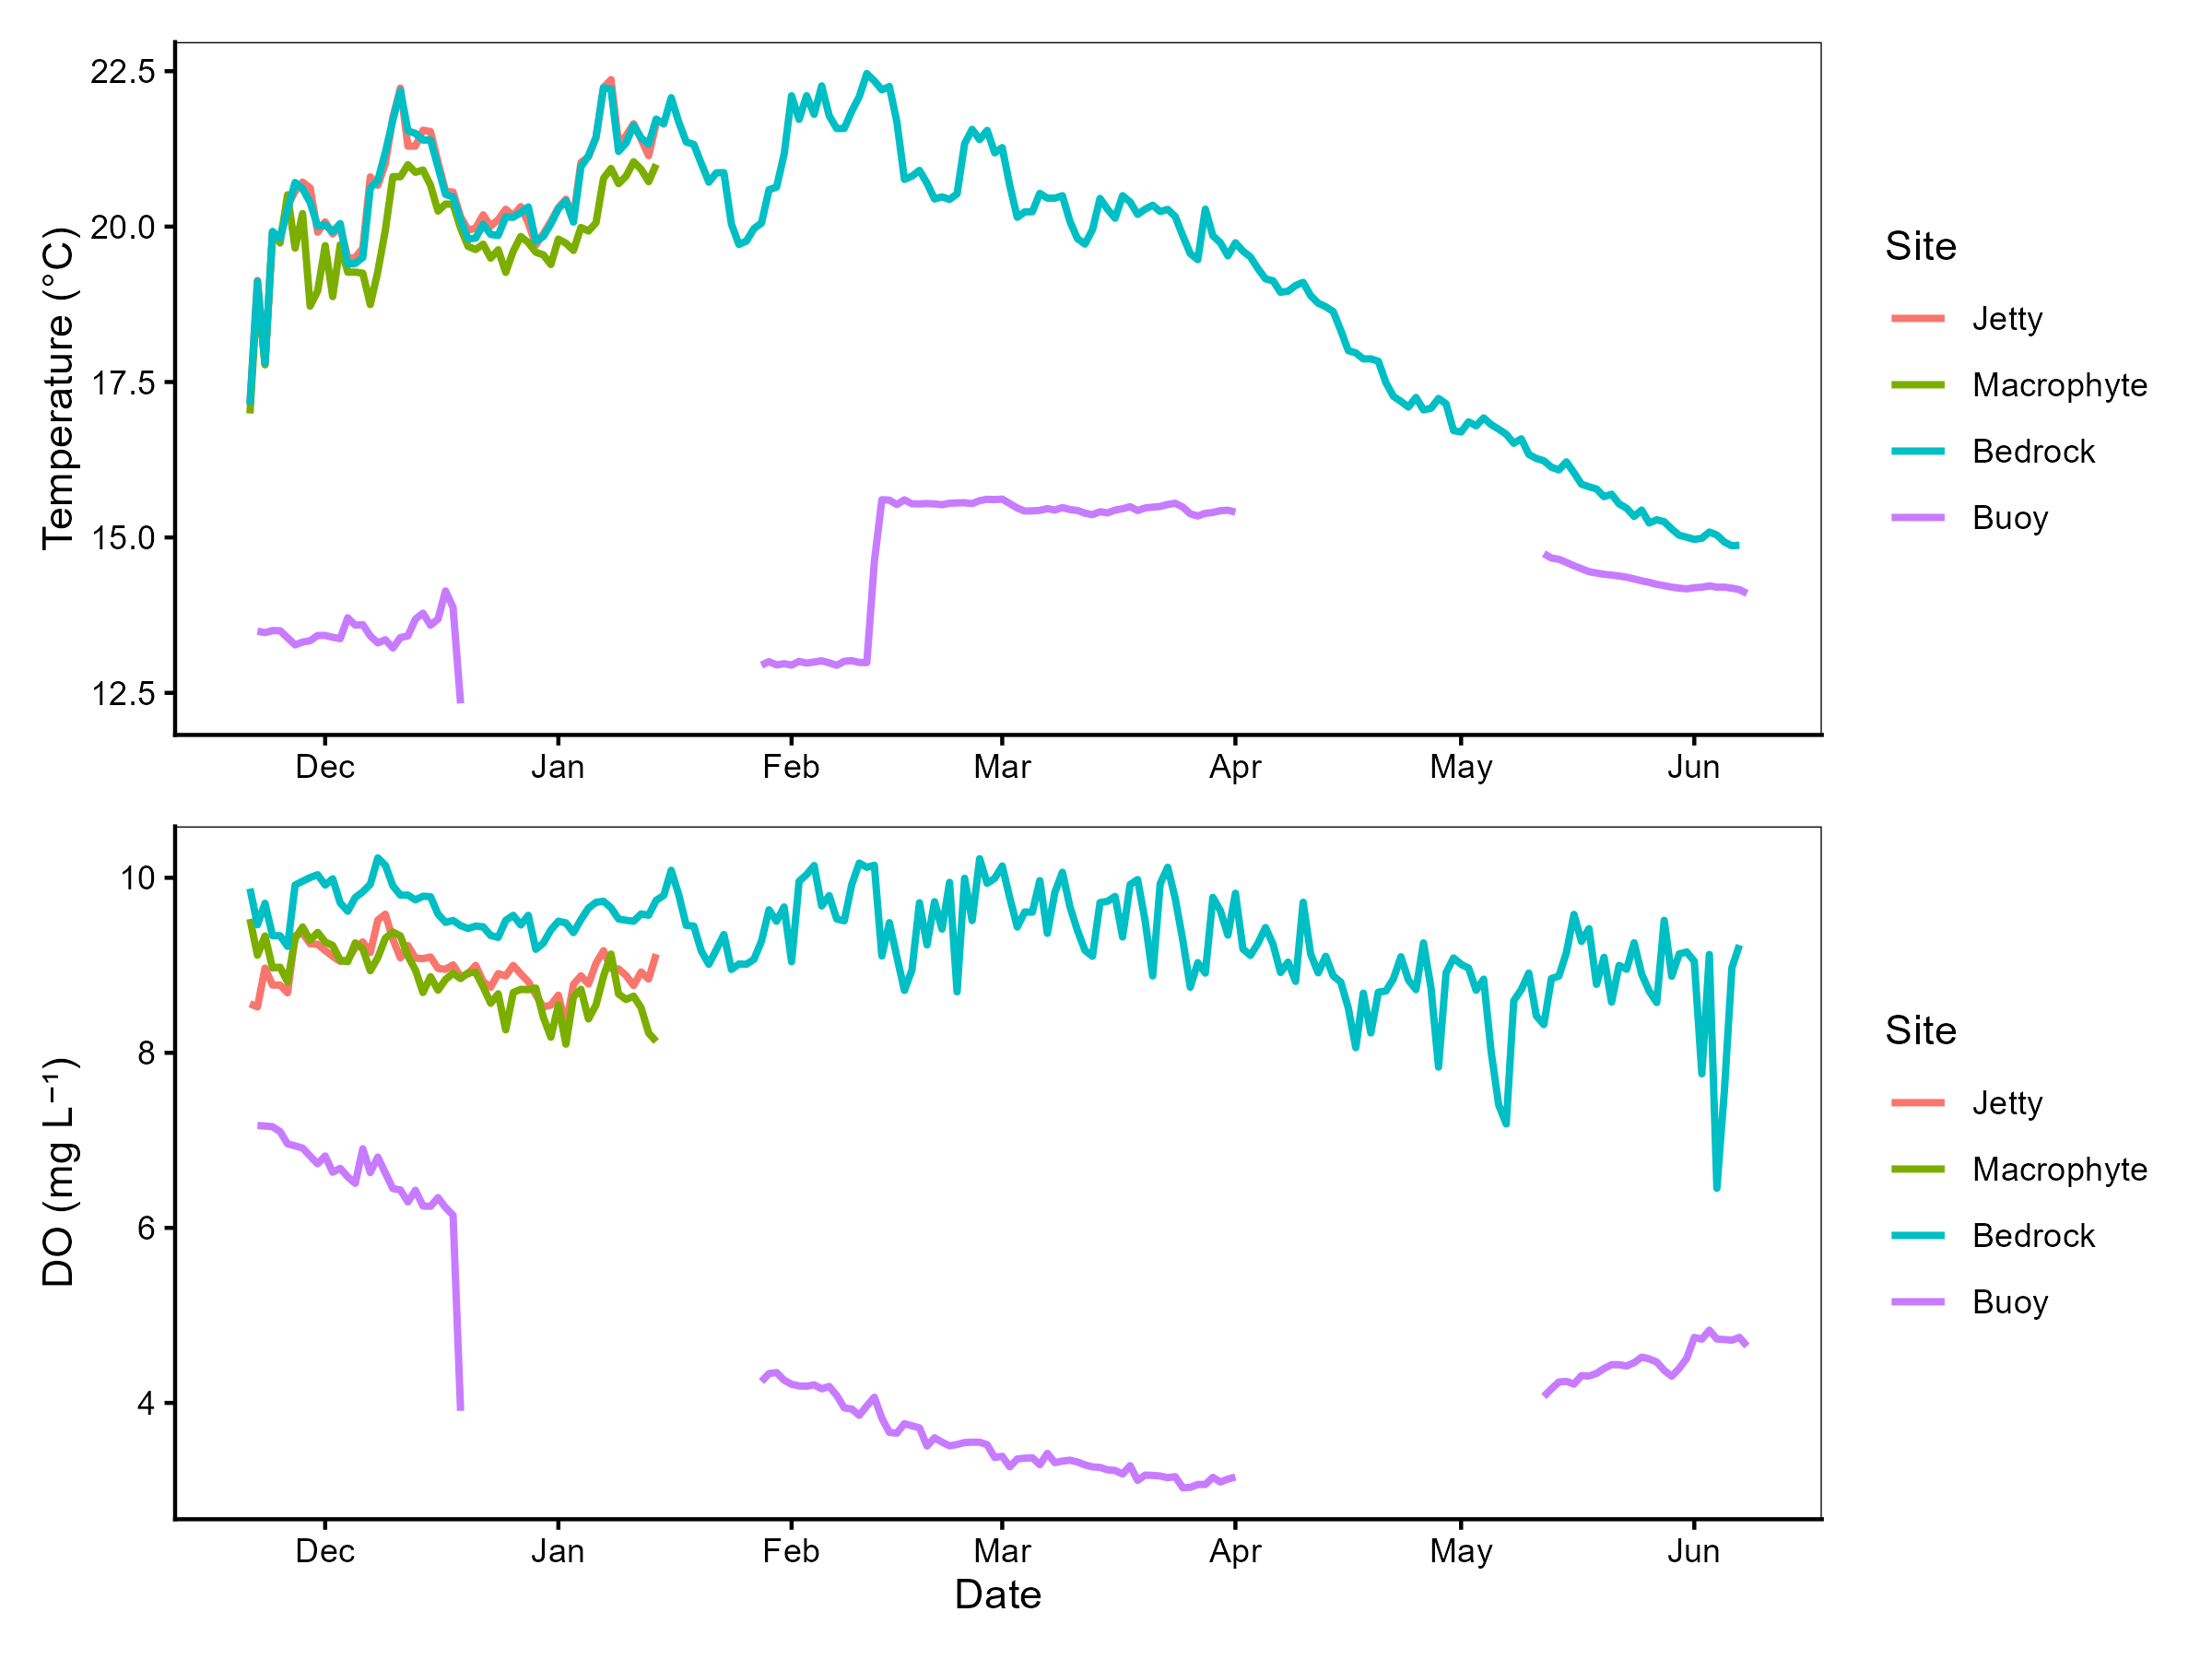
\includegraphics[width=0.8\linewidth,height=\textheight,keepaspectratio]{outputs/fig-deep-combined.png}

}

\caption{\label{fig-deep-combined}Daily mean water temperature (top) and
dissolved oxygen (bottom) at deep stone piles, control sites, and the
lake monitoring buoy \textless{} 1m. Period: 2025-11-22 to 2026-06-8.
Buoy data derived from CTD cast collected by LimnoTrack (Moore and
McBride 2026).}

\end{figure}%

Extending deployment across a depth gradient adds an important dimension
absent from the shallow shoreline work of Chapter 5. Kōura used stone
piles across the full depth gradient from the shallow nearshore to 9 m
depth. As surface waters warm in summer, shallow refuges may exceed
kōura thermal tolerance while deeper structures remain within the
habitable temperature range, and stay above the anoxic hypolimnion.
Structures spanning this gradient therefore allow kōura to track the
habitable depth window as it shifts seasonally between thermal and
oxygen constraints. Stone piles at depth therefore address not only
structural habitat availability but also the habitat compression dynamic
identified as a key stressor in the Rotorua Te Arawa Lakes. The observed
suppression of macrophytes suggests an additional co-benefit: by
preventing macrophyte growth, stone piles also prevent the buildup of
organic matter that would otherwise die off, sink to depth, and
intensify deep-water deoxygenation through a pathway distinct from
thermal stratification. Stone piles could also potentially create
connectivity between shallow and deep refuges in overgrown littoral
zones, though this warrants further investigation.

\section{Kōura monitoring approaches}\label{koura-monitoring-approaches}

The choice of monitoring method depends on what question is being asked.
Methods that sample a general area answer ``how many kōura are present
in this location?'' while active, site specific methods answer ``are
kōura using this structure?''. These are distinct questions, and
selecting the right monitoring method for each is relevant. Traditional
Māori harvesting methods using tau kōura with whakaweku (bundles of
bracken fern \emph{Pteridium esculentum}) have proven effective for
kōura monitoring in lakes and stream habitats (Kusabs and Quinn 2009;
Kusabs et al. 2018). In the shallow wave-exposed zone of a lake, however
whakaweku is less suitable as wave action destabilises the bundles,
reducing their effectiveness as a consistent shelter substrate. A
further limitation in the context of this thesis is that whakaweku
creates habitat. Using it to assess whether stone piles attract kōura
would confound the monitoring tool with the intervention, making it
impossible to determine whether kōura are responding to the stone pile
or the whakaweku itself. Passive netting with single-winged fyke nets
and baited box traps was therefore used throughout Chapters 3 and 5. Box
traps were baited with trout flesh in Chapter 3 and catfish flesh in
Chapter 5. When comparing catches at Lake Rotoiti sites, no difference
was found between bait types. This was expected as kōura scavenge
carcasses of dead predator fish without bias towards native or
non-native species (MacNeil et al. 2025). Trout as bait yielded a CPUE
of 0.682 kōura per trap per night and catfish bait 0.638 kōura per trap
per night. Unbaited fyke nets had a notably higher CPUE of 2.71 kōura
per trap per night in the same lake, consistent with their larger net
opening and longer fishing lead. However, 24-hour passive netting
provides an approximation of local abundance rather than direct evidence
of habitat use. Trap catches alone cannot determine whether kōura are
actively using stone piles or are simply present in the surrounding
area. For Chapter 5, higher catches near stone piles were therefore
interpreted as indicating greater habitat use of the structures. In
structurally complex habitats, fyke nets must be placed flat on the
sediment to fish effectively; on rocky substrates this is often not
possible, and kōura may pass beneath the net opening entirely. At the
deep structures built in Lake Rotoiti, more active monitoring approaches
were applied including spotlighting, ROV surveys and human dive surveys.
These methods allow direct observation of kōura using the structures and
are easier to execute over depth than netting.

Looking forward, it would be valuable to develop and trial additional
monitoring techniques including environmental DNA (eDNA), remote
underwater video (RUV), baited remote underwater video (BRUV), and
passive acoustic monitoring. Comparative studies suggest that trapping,
RUV, BRUV perform similarly for crayfish detection while eDNA has failed
to detect crayfish in similar stream systems (Harwood et al. 2025,
2026). Conversely, eDNA has detected invasive crayfish in lakes where
trapping alone could not (Dougherty et al. 2016), suggesting it may be
better suited to lake-scale presence-absence assessments than to
evaluate kōura use of specific structures. Passive acoustics offer a
complementary approach as crayfish produce distinctive sounds during
movement and feeding, and acoustic methods have shown potential for
identifying crayfish behaviour in field and laboratory settings
(Buscaino et al. 2012; De Vita et al. 2023). Application in marine
systems has advanced further, including detection of spiny lobsters over
great distances (Jézéquel et al. 2020, 2023); whether passive acoustic
monitoring is sensitive enough to detect kōura activity in the complex
acoustic environment of a lake littoral zone remains untested.

\section{What habitat enhancement can and cannot
fix}\label{what-habitat-enhancement-can-and-cannot-fix}

Chapter 3 showed that kōura were most consistently associated with
complex rocky habitats and riparian vegetation. Locations where this
substrate has been lost or never existed are therefore logical
candidates for stone pile deployment. Chapter 4 confirmed that stability
and structural complexity are the decisive factors in kōura shelter
selection, and stone piles deliver both. In lakes where populations are
declining, stone piles can help a remnant population persist and create
habitat stepping stones that lower the cost of dispersal between
patches, keeping populations more connected while broader lake
conditions improve. Stone piles can also physically suppress invasive
macrophytes at the placement site as demonstrated in the deep Rotoiti
case study. Chapter 5 demonstrates that stone piles represent a specific
type of intervention that operates differently from stressor removal.
Unlike water quality improvement or catfish management, structural
habitat addition does not require the stressors to be controlled before
it delivers benefits for kōura. Stone piles function as a buffer against
stressors that cannot be eliminated at lake scale. Catfish eradication
from lakes Rotoiti and Rotorua is not feasible without measures that
would be catastrophic for native fish communities, and thermal
stratification will intensify under continued climate warming (Woolway
et al. 2021; Lee et al. 2025). When these stressors cannot be removed
habitat enhancement can become a practical management tool whose value
increases when conditions worsen.

Whether habitat enhancement delivers population-level benefits depends
on whether habitat availability is genuinely limiting. In a Norwegian
lake where muddy substrates limited noble crayfish (\emph{Astacus
astacus}) distribution, adding rocky substrate to previously
unproductive areas resulted in colonisation and improved harvest
(Johnsen and Taugbøl 2008). In that system, habitat was the constraint,
and removing it produced a clear response. Similarly, structure
additions to streams have been shown to improve success of crayfish
restocking efforts (Huolila et al. 1997). In both cases, suitable
habitat was the limiting factor that limited the crayfish population.
The situation in the Rotorua Te Arawa Lakes is more complex, habitat
availability is not independently limiting but becomes limiting in
combination with other stressors. Thermal stratification and invasive
macrophytes compress kōura into a narrow littoral zone, and catfish
predation within that zone forces kōura into refuges, which are scarce
in the predominant sandy littoral zone of Lake Rotoiti.

The lack of suitable habitat is one of the compounding stressors, and
addressing it alone will not produce the same clear population response.
If dissolved oxygen drops below kōura tolerance, structure is
irrelevant, as demonstrated by the anoxic event in Lake Ōkaro. If
catfish pressure remains high, stone piles improve survival odds but
cannot prevent the continuous suppression from the impacts of fear and
predation.

Habitat enhancement therefore sets a ceiling defined by the other
stressors. Chapter 3 showed that the lakes with the best habitat and the
best water quality, most complex habitat, and no catfish support the
highest kōura abundance. As catfish can probably not be eradicated at
lake scale and thermal stratification will intensify under continued
climate warming, habitat enhancement must therefore be pursued not as
final step in a linear recovery sequence, but as a parallel intervention
whose benefit grows as the other stressore intensify.

\section{Future direction}\label{future-direction}

The findings of this thesis open several direction for future research
and management, ranging from individual deployments to lake-wide kōura
restoration strategies.

\subsection{Scaling deployment}\label{scaling-deployment}

The five stone pile sites monitored in Chapter 5 represent a
proof-of-concept deployment rather than a management-scale intervention.
The positive but non-significant trend in kōura abundance suggest that
the 18-month monitoring period was insufficient to detect
population-level responses. Continued monitoring of the existing Rotoiti
stone piles would determine whether the positive trends continue and
what the long term effect is without requiring new deployments.

Beyond continued monitoring, scaling deployment to additional sites and
lakes would test whether the Rotoiti results are generalised across the
Te Arawa system. Lake Rotorua, which has also declining kōura
populations and limited natural rocky habitats would be logical next
deployment location. The deep stone pile case study in this chapter
demonstrated that deployment across a depth gradient extends the range
of conditions under which kōura can use the structures and further
deployment should incorporate this principle. Standardised monitoring
protocols across sites, including spotlighting, fyke netting, and ROV
surveys, would allow for across-lake comparison of the habitat
enhancement as a management tool.

\subsection{Community contributions}\label{community-contributions}

One of the practical strengths of stone pile deployment is that
construction does not require specialist equipment or expertise. Both
the Rotoiti and Ōkaro deployments in this thesis were built by hand
using locally sourced materials, demonstrating that this kind of
restoration work is accessible to a wide range of participants.

Residents living along the lakes could contribute directly, for example
by replacing unproductive hard structures, like retaining walls that
provide no habitat value, with stones and rocks or by placing stones
under jetties where they are out of the way of boating and swimming yet
provide effective shelter for kōura. Some residents around the Rotorua
Te Arawa Lakes have already independently built kōura habitat structures
using similar principles (Figure~\ref{fig-koura-structures-diy}),
demonstrating both the appeal and feasibility of community-led habitat
enhancement. Future community contributions would benefit from using
natural materials that will not degrade over time, and from maximising
crevice diversity, as the more hiding places the structures creates, the
wider the range of kōura life stages it can support. Stones in the 100-
300 mm range, as used in this study, provide abundant shelter space when
stacked together, are simple to deploy and persist in the lake without
introducing pollutants.

\begin{figure}

\centering{

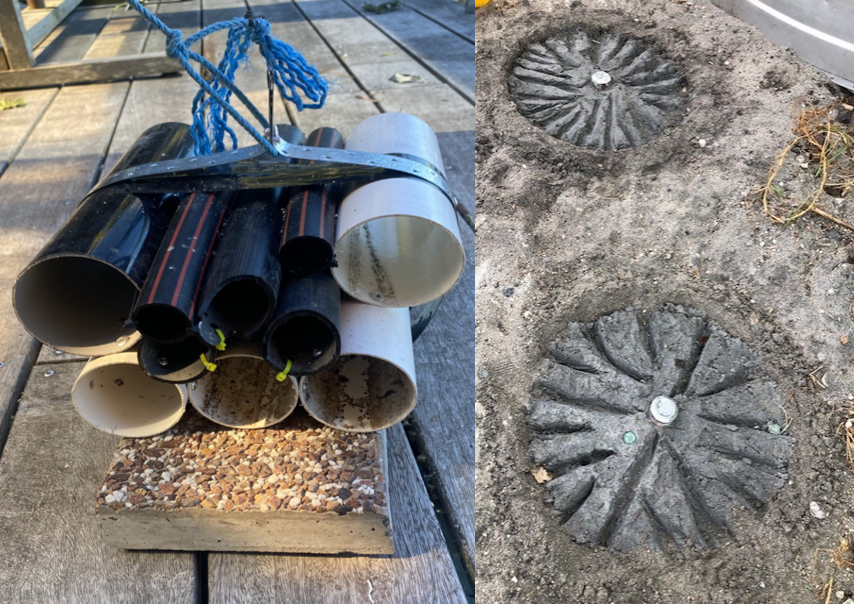
\includegraphics[width=0.65\linewidth,height=\textheight,keepaspectratio]{images/Koura_structures_diy.png}

}

\caption{\label{fig-koura-structures-diy}Home made kōura habitats by
local residents. Left: Kōura pipes by Mark Thomson Lake Rotoiti. Right:
Kōura weels by Mark Robinson Lake Tarawera.}

\end{figure}%

\subsection{Te Arawa and cultural
dimension}\label{te-arawa-and-cultural-dimension}

Kōura are taonga, a treasured species with deep cultural significance
for Te Arawa iwi. The decline documented in this thesis is not only an
ecological loss but a cultural one. Increasing shelter availability may
attract kōura and support population recovery, with potential benefits
for cultural practices. Little tau kōura harvesting currently occurs at
Cherry Bay (Ōkahuroroa Bay) in Lake Rotoiti where regular monitoring
using whakaweku has potentially already created a degree of structural
complexity in the bay. Whether increased habitat provision at scale
could support renewed harvest activity in areas like this is a question
for future research and management to consider together with Te Arawa.

A hard but honest assessment is warrented regarding the restoration of
cultural kōura harvest in Lake Rotoiti. Given the compounding effects of
multiple stressore, and the expectation that both climate change and the
threat of invasive species will persist, the honest conclusion of this
thesis is that kōura will likely persist in the these lakes but that
lake-wide populations are unlikely to reach the abundance historically
required for cultural harvest while catfish predation remains
persistent. Catfish and kōura may eventually reach a new predator-prey
equaribium, particularly if active catfish control efforts cannot be
sustained indefinitely. In this context, management priorities may be
better directed toward protecting kōura populations that remain strong
in lakes without catfish, like Rotomā, Ōkāreka, and Tarawera, by
preventing the spread of catfish and invasive macrophytes into these
systems, rather than solely focusing on recovery in already
catfish-invaded lakes.

\section{Conclusion}\label{conclusion-1}

Kōura populations in the Rotorua Te Arawa Lakes have declined by up to
76-91 \% since 2003, and this thesis set out to determine whether
habitat enhancement could offer a practical mean of supporting them.

The findings confirm that kōura decline is driven by multiple stressors
acting together rather than in isolation. Non-consumptive, fear induced
behavioural suppression from catfish predation compounds with thermal
stratification that compresses suitable habitat into the shallow
littoral zone, precisely where catfish predation pressure is greatest.
This leaves kōura needing for refuge, and it is this compounding dynamic
that structural habitat enhancement directly addresses.

Stone piles will not remove catfish from the lakes or reverse thermal
stratification. The evidence presented here shows that kōura
consistently and rapidly find and use these structures, that stone piles
provide refuge without attracting the predator, and their value is
seasonal, with greatest need in summer and autumn. Whether this
translates into a detectable population-level recovery will take longer
than 18 months, but the direction of the evidence is consistent and
encouriging.

On its own stone pile deployment will likely never restore lake-wide
populations to the abundance needed for cultural harvest, while catfish
predation persists. This is a hard conclusion, but an honest one. What
structural habitat enhancement can do is buffer the worst effects of
compounding stressors and help keep local populations in a condition
from which recovery remains possible, when broader conditions improve in
the future. In a system where the primary drivers of decline can not be
removed, giving kōura somewhere to hide is not a complete solution, but
it is a meaningful and actionable one.

\chapter*{References}\label{references}
\addcontentsline{toc}{chapter}{References}

\markboth{References}{References}
\begingroup
\small
\setlength{\parskip}{2pt}
\setlength{\itemsep}{0pt}

\protect\phantomsection\label{refs}
\begin{CSLReferences}{1}{1}
\bibitem[\citeproctext]{ref-Abrams2000}
Abrams PA (2000) The evolution of predator-prey interactions: Theory and
evidence. Annual Review of Ecology and Systematics 31:79--105.
\url{https://doi.org/10.1146/annurev.ecolsys.31.1.79}

\bibitem[\citeproctext]{ref-Achtymichuk2025}
Achtymichuk GH, Fish KM, Ferrari MCO (2025) The power of concentration:
Antipredator responses to diluted frozen crayfish alarm cues provide
insights on ecologically relevant concentrations and updates to
methodology. PLOS One 20:e0340001.
\url{https://doi.org/10.1371/journal.pone.0340001}

\bibitem[\citeproctext]{ref-Adams2007}
Adams SB (2007) Direct and indirect effects of channel catfish
({\emph{Ictalurus punctatus}}) on native crayfishes ({Cambaridae}) in
experimental tanks. The American Midland Naturalist 158:85--96.
\url{https://doi.org/10.1674/0003-0031(2007)158\%5B85:daieoc\%5D2.0.co;2}

\bibitem[\citeproctext]{ref-Adams2014}
Adams SB (2014) Crayfish use of trash versus natural cover in incised,
sand-bed streams. Environmental Management 53:382--392.
\url{https://doi.org/10.1007/s00267-013-0197-3}

\bibitem[\citeproctext]{ref-Albertson2018}
Albertson LK, Daniels MD (2018) Crayfish ecosystem engineering effects
on riverbed disturbance and topography are mediated by size and
behavior. Freshwater Science 37:836--844.
\url{https://doi.org/10.1086/700884}

\bibitem[\citeproctext]{ref-Angilletta2004}
Angilletta MJ, Steury TD, Sears MW (2004) Temperature, growth rate, and
body size in ectotherms: Fitting pieces of a life-history puzzle.
Integrative and Comparative Biology 44:498--509.
\url{https://doi.org/10.1093/icb/44.6.498}

\bibitem[\citeproctext]{ref-Appelberg1993}
Appelberg M, Soederbaeck B, Odelstroem T (1993) Predator detection and
perception of predation risk in the crayfish {\emph{Astacus astacus}} l.
Nordic journal of freshwater research 68:55--62

\bibitem[\citeproctext]{ref-Baine2001}
Baine M (2001) Artificial reefs: A review of their design, application,
management and performance. Ocean \& Coastal Management 44:241--259.
\url{https://doi.org/10.1016/s0964-5691(01)00048-5}

\bibitem[\citeproctext]{ref-BanksLeite2020}
Banks-Leite C, Ewers RM, Folkard-Tapp H, Fraser A (2020) Countering the
effects of habitat loss, fragmentation, and degradation through habitat
restoration. One Earth 3:672--676.
\url{https://doi.org/10.1016/j.oneear.2020.11.016}

\bibitem[\citeproctext]{ref-Barnes1996}
Barnes GE (1996) The biology and general ecology of the brown bullhead
catfish (\emph{ameiurus nebulosus}) in {Lake Taupo}. Master's thesis,
University of Waikato

\bibitem[\citeproctext]{ref-Barnes2003}
Barnes GE, Hicks BJ (2003) Brown bullhead catfish ({\emph{Ameiurus
nebulosus}}) in {Lake Taupo}. In: Managing invasive freshwater fish in
{New Zealand}: Proceedings of a workshop hosted by {Department of
Conservation}, 10-12 may 2001, {Hamilton}. Department of Conservation

\bibitem[\citeproctext]{ref-Bates2015}
Bates D, Mächler M, Bolker B, Walker S (2015) Fitting linear
mixed-effects models using {lme4}. Journal of Statistical Software
67:1--48. \url{https://doi.org/10.18637/jss.v067.i01}

\bibitem[\citeproctext]{ref-Beattie2018}
Beattie MC, Moore PA (2018) Predator recognition of chemical cues in
crayfish: Diet~and experience influence the ability
to~detect~predation~threats. Behaviour 155:505--530.
\url{https://doi.org/10.1163/1568539x-00003501}

\bibitem[\citeproctext]{ref-Beck1995}
Beck MW (1995) Size-specific shelter limitation in stone crabs: A test
of the demographic bottleneck hypothesis. Ecology 76:968--980.
\url{https://doi.org/10.2307/1939360}

\bibitem[\citeproctext]{ref-Bhateria2016}
Bhateria R, Jain D (2016) Water quality assessment of lake water: A
review. Sustainable Water Resources Management 2:161--173.
\url{https://doi.org/10.1007/s40899-015-0014-7}

\bibitem[\citeproctext]{ref-Blair2009}
Blair JM, Hicks BJ (2009) An investigation to determine origin: Age and
otolith chemistry of a brown bullhead catfish (\emph{ameiurus
nebulosus}) found at {Okawa Bay, Lake Rotoiti}. Centre for Biodiversity;
Ecology Research, University of Waikato, Hamilton, New Zealand

\bibitem[\citeproctext]{ref-Blake1993}
Blake MA, Hart PJB (1993) The behavioural responses of juvenile signal
crayfish {\emph{Pacifastacus leniusculus}} to stimuli from perch and
eels. Freshwater Biology 29:89--97.
\url{https://doi.org/10.1111/j.1365-2427.1993.tb00747.x}

\bibitem[\citeproctext]{ref-Blanchfield2026}
Blanchfield PJ, Rodrigues TH, MacNeil C, et al (2026) Invadingbrown
bullhead catfish (ameiurus nebulosus) show thermal niche rigidity and
benthic niche plasticity: Implications for management. Biological
Invasions. \url{https://doi.org/10.1007/s10530-026-03877-5}

\bibitem[\citeproctext]{ref-Bolker2009}
Bolker BM, Brooks ME, Clark CJ, et al (2009) Generalized linear mixed
models: A practical guide for ecology and evolution. Trends in Ecology
\& Evolution 24:127--135.
\url{https://doi.org/10.1016/j.tree.2008.10.008}

\bibitem[\citeproctext]{ref-Bonacina2023}
Bonacina L, Fasano F, Mezzanotte V, Fornaroli R (2023) Effects of water
temperature on freshwater macroinvertebrates: A systematic review.
Biological Reviews 98:191--221. \url{https://doi.org/10.1111/brv.12903}

\bibitem[\citeproctext]{ref-Bronmark2012}
Brönmark C, Hansson L-A (2012) Chemical ecology in aquatic systems.
Oxford University Press

\bibitem[\citeproctext]{ref-Brooks2017}
Brooks M, Bolker B, Kristensen K, et al (2017)
\href{https://doi.org/10.32614/cran.package.glmmtmb}{glmmTMB:
Generalized linear mixed models using template model builder}. CRAN:
Contributed Packages

\bibitem[\citeproctext]{ref-Broughton2017}
Broughton RJ, Marsden ID, Hill JV, Glover CN (2017) Behavioural,
physiological and biochemical responses to aquatic hypoxia in the
freshwater crayfish, {\emph{Paranephrops zealandicus}}. Comparative
Biochemistry and Physiology Part A: Molecular \& Integrative Physiology
212:72--80. \url{https://doi.org/10.1016/j.cbpa.2017.07.013}

\bibitem[\citeproctext]{ref-Brown2004}
Brown GE, Poirier J-F, Adrian JC (2004) Assessment of local predation
risk: The role of subthreshold concentrations of chemical alarm cues.
Behavioral Ecology 15:810--815.
\url{https://doi.org/10.1093/beheco/arh084}

\bibitem[\citeproctext]{ref-Brown2009}
Brown LA (2009) \href{http://hdl.handle.net/10179/1168}{Habitat
determinants and predatory interactions of the endemic freshwater
crayfish (koura, {\emph{Paranephrops planifrons}}) in the lower {North
Island}, {New Zealand}}. Master's thesis, Massey University

\bibitem[\citeproctext]{ref-Bunch2010}
Bunch AJ, Allen MS, Gwinn DC (2010) Spatial and temporal hypoxia
dynamics in dense emergent macrophytes in a {Florida} lake. Wetlands
30:429--435. \url{https://doi.org/10.1007/s13157-010-0051-9}

\bibitem[\citeproctext]{ref-Burkner2017}
Bürkner P-C (2017) {brms}: An {R} package for {B}ayesian multilevel
models using {Stan}. Journal of Statistical Software 80:
\url{https://doi.org/10.18637/jss.v080.i01}

\bibitem[\citeproctext]{ref-Burkner2018}
Bürkner P-C (2018) Advanced {B}ayesian multilevel modeling with the {R}
package brms. The R Journal 10:395.
\url{https://doi.org/10.32614/rj-2018-017}

\bibitem[\citeproctext]{ref-Burnham2002}
Burnham KP, Anderson DR (2002)
\href{https://doi.org/10.1007/978-0-387-22456-5_6}{Advanced issues and
deeper insights}. In: Model selection and multimodel inference: A
practical information-theoretic approach. Springer, New York, NY, pp
267--351

\bibitem[\citeproctext]{ref-Burton2017}
Burton T (2017)
\href{https://researchcommons.waikato.ac.nz/server/api/core/bitstreams/ff0cbe45-8f02-4ea7-9118-4343a7869980/content}{Lake
weed and the {Rotorua Te Arawa Lakes} then and now}

\bibitem[\citeproctext]{ref-Buscaino2012}
Buscaino G, Filiciotto F, Buffa G, et al (2012) The underwater acoustic
activities of the red swamp crayfish \textless i\textgreater procambarus
clarkii\textless/i\textgreater. The Journal of the Acoustical Society of
America 132:1792--1798. \url{https://doi.org/10.1121/1.4742744}

\bibitem[\citeproctext]{ref-Butler1999}
Butler M, MacDiarmid A, Booth J (1999) The cause and consequence of
ontogenetic changes in social aggregation in {New Zealand} spiny
lobsters. Marine Ecology Progress Series 188:179--191.
\url{https://doi.org/10.3354/meps188179}

\bibitem[\citeproctext]{ref-Capinha2013}
Capinha C, Larson ER, Tricarico E, et al (2013) Effects of climate
change, invasive species, and disease on the distribution of native
{European} crayfishes. Conservation Biology 27:731--740.
\url{https://doi.org/10.1111/cobi.12043}

\bibitem[\citeproctext]{ref-Carthey2014}
Carthey AJR, Banks PB (2014) Naïveté in novel ecological interactions:
Lessons from theory and experimental evidence. Biological Reviews
89:932--949. \url{https://doi.org/10.1111/brv.12087}

\bibitem[\citeproctext]{ref-Chambers1987}
Chambers PA (1987) Nearshore occurrence of submersed aquatic macrophytes
in relation to wave action. Canadian Journal of Fisheries and Aquatic
Sciences 44:1666--1669. \url{https://doi.org/10.1139/f87-204}

\bibitem[\citeproctext]{ref-Childress2001}
Childress MJ, Herrnkind WF (2001) The guide effect influence on the
gregariousness of juvenile caribbean spiny lobsters. Animal Behaviour
62:465--472. \url{https://doi.org/10.1006/anbe.2001.1760}

\bibitem[\citeproctext]{ref-Clapcott2018}
Clapcott J, Ataria J, Hepburn C, et al (2018) {Mātauranga Māori}:
Shaping marine and freshwater futures. New Zealand Journal of Marine and
Freshwater Research 52:457--466.
\url{https://doi.org/10.1080/00288330.2018.1539404}

\bibitem[\citeproctext]{ref-Clay2017}
Clay M, Stoeckel J, Helms B (2017) The role of abiotic and biotic cues
in burrow habitat selection by juvenile crayfish. Behaviour
154:1177--1196. \url{https://doi.org/10.1163/1568539x-00003463}

\bibitem[\citeproctext]{ref-Clinchy2013}
Clinchy M, Sheriff MJ, Zanette LY (2012) Predator‐induced stress and the
ecology of fear. Functional Ecology 27:56--65.
\url{https://doi.org/10.1111/1365-2435.12007}

\bibitem[\citeproctext]{ref-Coffey1988}
Coffey BT, Clayton JS (1988) Contrasting deep-water macrophyte
communities in two highly transparent {New Zealand} lakes and their
possible association with freshwater crayfish, {\emph{Paranephrops}}
spp. New Zealand Journal of Marine and Freshwater Research 22:225--230.
\url{https://doi.org/10.1080/00288330.1988.9516294}

\bibitem[\citeproctext]{ref-Cole2014}
Cole JW, Deering CD, Burt RM, et al (2014) {Okataina Volcanic Centre,
Taupo Volcanic Zone, New Zealand}: A review of volcanism and synchronous
pluton development in an active, dominantly silicic caldera system.
Earth-Science Reviews 128:1--17.
\url{https://doi.org/10.1016/j.earscirev.2013.10.008}

\bibitem[\citeproctext]{ref-Collier1997}
Collier KJ, Parkyn SM, Rabeni CF (1997) Koura: A keystone species. Water
and Atmosphere 5:18--20

\bibitem[\citeproctext]{ref-Cooke2022}
Cooke SJ, Frempong-Manso A, Piczak ML, et al (2022) A freshwater
perspective on the {United Nations} decade for ecosystem restoration.
Conservation Science and Practice 4:e12787.
\url{https://doi.org/10.1111/csp2.12787}

\bibitem[\citeproctext]{ref-Cooke2023}
Cooke SJ, Piczak ML, Vermaire JC, Kirkwood AE (2023) On the troubling
use of plastic 'habitat' structures for fish in freshwater ecosystems
--- or --- when restoration is just littering. FACETS 8:1--19.
\url{https://doi.org/10.1139/facets-2022-0210}

\bibitem[\citeproctext]{ref-Crandall2008}
Crandall KA, Buhay JE (2008) Global diversity of crayfish ({Astacidae,
Cambaridae}, and {Parastacidae} --- {Decapoda}) in freshwater.
Hydrobiologia 595:295--301.
\url{https://doi.org/10.1007/s10750-007-9120-3}

\bibitem[\citeproctext]{ref-Crandall2017}
Crandall KA, De Grave S (2017) An updated classification of the
freshwater crayfishes (decapoda: Astacidea) of the world, with a
complete species list. Journal of Crustacean Biology 37:615--653.
\url{https://doi.org/10.1093/jcbiol/rux070}

\bibitem[\citeproctext]{ref-Creed2004}
Creed RP, Reed JM (2004) Ecosystem engineering by crayfish in a
headwater stream community. Journal of the North American Benthological
Society 23:224--236.
\url{https://doi.org/10.1899/0887-3593(2004)023\%3C0224:EEBCIA\%3E2.0.CO;2}

\bibitem[\citeproctext]{ref-Danilovic2022}
Danilović M, Maguire I, Füreder L (2022) Overlooked keystone species in
conservation plans of fluvial ecosystems in {Southeast Europe}: A review
of native freshwater crayfish species. Knowledge \& Management of
Aquatic Ecosystems 21. \url{https://doi.org/10.1051/kmae/2022016}

\bibitem[\citeproctext]{ref-Dawkins1979}
Dawkins R, Krebs JR (1979) Arms races between and within species.
Proceedings of the Royal Society of London B Biological Sciences
205:489--511. \url{https://doi.org/10.1098/rspb.1979.0081}

\bibitem[\citeproctext]{ref-DeVita2023}
De Vita C, Mauro M, Vazzana M, et al (2023) Acoustic signals and
behavior of the invasive freshwater crayfish cherax destructor (clark,
1936). Journal of Marine Science and Engineering 11:1147.
\url{https://doi.org/10.3390/jmse11061147}

\bibitem[\citeproctext]{ref-Dedual2002}
Dedual M (2002) Vertical distribution and movements of brown bullhead
(\emph{ameiurus nebulosus} {Lesueur} 1819) in {Motuoapa Bay, southern
Lake Taupo, New Zealand}. Hydrobiologia 483:129--135.
\url{https://doi.org/10.1007/978-94-017-0771-8_15}

\bibitem[\citeproctext]{ref-Dedual2019}
Dedual M (2019) Summary of the impacts and control methods of {Brown
Bullhead} catfish (\emph{ameiurus nebulosus} {Lesueur} 1815) in {New
Zealand} and overseas. Bay of Plenty Regional Council

\bibitem[\citeproctext]{ref-Devcich1979}
Devcich AA (1979) An ecological study of \emph{paranephrops planifrons}
{White} ({Decapoda: Parastacidae}) in {Lake Rotoiti, North Island}. PhD
thesis, University of Waikato

\bibitem[\citeproctext]{ref-Dickson2023}
Dickson J, Franken O, Watson MS, et al (2023) Who lives in a pear tree
under the sea? A first look at tree reefs as a complex natural
biodegradable structure to enhance biodiversity in marine systems.
Frontiers in Marine Science 10:1213790.
\url{https://doi.org/10.3389/fmars.2023.1213790}

\bibitem[\citeproctext]{ref-Doherty2016}
Doherty TS, Glen AS, Nimmo DG, et al (2016) Invasive predators and
global biodiversity loss. Proceedings of the National Academy of
Sciences 113:11261--11265. \url{https://doi.org/10.1073/pnas.1602480113}

\bibitem[\citeproctext]{ref-Dougherty2016}
Dougherty MM, Larson ER, Renshaw MA, et al (2016)
Environmental\textless scp\textgreater DNA\textless/scp\textgreater(\textless scp\textgreater eDNA\textless/scp\textgreater)
detects the invasive rusty crayfish\textless i\textgreater orconectes
rusticus\textless/i\textgreater at low abundances. Journal of Applied
Ecology 53:722--732. \url{https://doi.org/10.1111/1365-2664.12621}

\bibitem[\citeproctext]{ref-Driscoll2020}
Driscoll J, Kola M, Mathews L (2020) Perception of alarm cues influences
the outcome of shelter competition in crayfish20. Ethology 126:584--592.
\url{https://doi.org/10.1111/eth.13011}

\bibitem[\citeproctext]{ref-Dudgeon2006}
Dudgeon D, Arthington AH, Gessner MO, et al (2006) Freshwater
biodiversity: Importance, threats, status and conservation challenges.
Biological Reviews 81:163--182.
\url{https://doi.org/10.1017/S1464793105006950}

\bibitem[\citeproctext]{ref-Dumelle2023}
Dumelle M, Kincaid T, Olsen AR, Weber M (2023) Spsurvey: Spatial
sampling design and analysis in {R}. Journal of Statistical Software
105: \url{https://doi.org/10.18637/jss.v105.i03}

\bibitem[\citeproctext]{ref-Ehlman2019}
Ehlman SM, Trimmer PC, Sih A (2019) Prey responses to exotic predators:
Effects of old risks and new cues. The American Naturalist 193:575--587.
\url{https://doi.org/10.1086/702252}

\bibitem[\citeproctext]{ref-Engels2014}
Engels B (2014)
\href{https://doi.org/10.32614/cran.package.xnomial}{{XNomial}: Exact
goodness-of-fit test for multinomial data with fixed probabilities}.
CRAN: Contributed Packages

\bibitem[\citeproctext]{ref-EsquivelMuelbert2026}
Esquivel-Muelbert JR, Fontoura L, Zawada K, et al (2026) The natural
architecture of oyster reefs maximizes recruit survival. Nature
652:393--397. \url{https://doi.org/10.1038/s41586-026-10103-8}

\bibitem[\citeproctext]{ref-Feldmann1994}
Feldmann RM, Pole M (1994) A new species of {\emph{Paranephrops}}
{White}, 1842: A fossil freshwater crayfish ({Decapoda}: {Parastacidae})
from the {Manuherikia Group} ({Miocene}), {Central Otago}, {New
Zealand}. New Zealand Journal of Geology and Geophysics 37:163--167.
\url{https://doi.org/10.1080/00288306.1994.9514611}

\bibitem[\citeproctext]{ref-Fetzner2019}
Fetzner JW (2019)
\href{https://www.invertebratezoology.org/NewAstacidea/infraorder.asp?io=Astacidea}{Crayfish
{Taxon Browser :: Infraorder Page}}

\bibitem[\citeproctext]{ref-Fielding1997}
Fielding AH, Bell JF (1997) A review of methods for the assessment of
prediction errors in conservation presence/absence models. Environmental
Conservation 24:38--49. \url{https://doi.org/10.1017/S0376892997000088}

\bibitem[\citeproctext]{ref-Figler2005}
Figler MH, Blank GS, Peeke HVS (2005) Shelter competition between
resident male red swamp crayfish {\emph{Procambarus clarkii}} ({Girard})
and conspecific intruders varying by sex and reproductive status. Marine
and Freshwater Behaviour and Physiology 38:237--248.
\url{https://doi.org/10.1080/10236240500376477}

\bibitem[\citeproctext]{ref-Figler1999}
Figler MH, Cheverton HM, Blank GS (1999) Shelter competition in juvenile
red swamp crayfish ({\emph{Procambarus clarkii}}): The influences of sex
differences, relative size, and prior residence. Aquaculture 178:63--75.
\url{https://doi.org/10.1016/s0044-8486(99)00114-3}

\bibitem[\citeproctext]{ref-Ford2005}
Ford T, Beitinger TL (2005) Temperature tolerance in the goldfish,
{\emph{Carassius auratus}}. Journal of Thermal Biology 30:147--152.
\url{https://doi.org/10.1016/j.jtherbio.2004.09.004}

\bibitem[\citeproctext]{ref-Francis2019}
Francis LB (2019)
\href{https://researchcommons.waikato.ac.nz/handle/10289/12746}{Evaluating
the effects of invasive brown bullhead catfish ({\emph{Ameiurus
nebulosus}}) on k{ō}ura (freshwater crayfish, {\emph{Paranephrops
planifrons}}) in {Lake Rotoiti}}. Master's thesis, University of Waikato

\bibitem[\citeproctext]{ref-Frehse2025}
Frehse F de A, Derviche P, Pereira FW, et al (2025) Artificial aquatic
habitats: A systematic literature review and new perspectives.
Hydrobiologia 852:1997--2012.
\url{https://doi.org/10.1007/s10750-024-05589-0}

\bibitem[\citeproctext]{ref-Froese2006}
Froese R (2006) Cube law, condition factor and weight-length
relationships: History, meta-analysis and recommendations. Journal of
Applied Ichthyology 22:241--253.
\url{https://doi.org/10.1111/j.1439-0426.2006.00805.x}

\bibitem[\citeproctext]{ref-Fry1948}
Fry FEJ, Hart JS (1948) Cruising speed of goldfish in relation to water
temperature. Journal of the Fisheries Research Board of Canada
7b:169--175. \url{https://doi.org/10.1139/f47-018}

\bibitem[\citeproctext]{ref-Gabry2025}
Gabry J, Češnovar R, Johnson A, Bronder S (2025)
\href{https://mc-stan.org/cmdstanr/}{Cmdstanr: R interface to 'CmdStan'}

\bibitem[\citeproctext]{ref-Gann2019}
Gann GD, McDonald T, Walder B, et al (2019) International principles and
standards for the practice of ecological restoration. {Second edition}.
Restoration Ecology 27: \url{https://doi.org/10.1111/rec.13035}

\bibitem[\citeproctext]{ref-Garron2024}
Garron C, Pangaud A, Taubaty M, et al (2024) Towards the development of
a standardized method to monitor lakeshore hydromorphological
restoration measures. Aquatic Conservation: Marine and Freshwater
Ecosystems 34: \url{https://doi.org/10.1002/aqc.4152}

\bibitem[\citeproctext]{ref-Geist2016}
Geist J, Hawkins SJ (2016) Habitat recovery and restoration in aquatic
ecosystems: Current progress and future challenges. Aquatic
Conservation: Marine and Freshwater Ecosystems 26:942--962.
\url{https://doi.org/10.1002/aqc.2702}

\bibitem[\citeproctext]{ref-Gelman1992}
Gelman A, Rubin DB (1992) Inference from iterative simulation using
multiple sequences. Statistical Science 7:457--472.
\url{https://doi.org/10.1214/ss/1177011136}

\bibitem[\citeproctext]{ref-Gherardi2011}
Gherardi F, Mavuti KM, Pacini N, et al (2011) The smell of danger:
Chemical recognition of fish predators by the invasive crayfish
{\emph{Procambarus clarkii}}. Freshwater Biology 56:1567--1578.
\url{https://doi.org/10.1111/j.1365-2427.2011.02595.x}

\bibitem[\citeproctext]{ref-Grayling2020}
Grayling S (2020) {Bay of Plenty Regional Pest Management Plan}
2011--2016 {Annual Report} for 2019/2020. Bay of Plenty Regional
Council, Whakatāne, New Zealand

\bibitem[\citeproctext]{ref-Greenaway1985}
Greenaway P (1985) Calcium balance and moulting in the {Crustacea}.
Biological Reviews 60:425--454

\bibitem[\citeproctext]{ref-Hamilton2005}
Hamilton D, McBride C, Uraoka T (2005) {Lake Rotoiti} fieldwork and
modeling to support considerations of {Ohau} channel diversion from
{Lake Rotoiti}. NIWA \& University of Waikato, Hamilton, New Zealand

\bibitem[\citeproctext]{ref-Hammond2006}
Hammond KS, Hollows JW, Townsend CR, Lokman PM (2006) Effects of
temperature and water calcium concentration on growth, survival and
moulting of freshwater crayfish, {\emph{Paranephrops zealandicus}}.
Aquaculture 251:271--279.
\url{https://doi.org/10.1016/j.aquaculture.2005.05.032}

\bibitem[\citeproctext]{ref-Hanski1998}
Hanski I (1998) Metapopulation dynamics. Nature 396:41--49.
\url{https://doi.org/10.1038/23876}

\bibitem[\citeproctext]{ref-Harding2009}
Harding JS, Clapcott JE, Quinn JM, et al (2009) Stream habitat
assessment protocols for wadeable rivers and streams of {New Zealand}.
School of Biological Sciences, University of Canterbury

\bibitem[\citeproctext]{ref-Harrison2018}
Harrison I, Abell R, Darwall W, et al (2018) The freshwater biodiversity
crisis. Science 362:1369. \url{https://doi.org/10.1126/science.aav9242}

\bibitem[\citeproctext]{ref-Hartig2016}
Hartig F (2016)
\href{https://doi.org/10.32614/cran.package.dharma}{{DHARMa}: Residual
diagnostics for hierarchical (multi-level / mixed) regression models}.
CRAN: Contributed Packages

\bibitem[\citeproctext]{ref-Hartig2024}
{Hartig F, Lohse L, leite M de S} (2024)
\href{https://cran.r-project.org/web/packages/DHARMa/index.html}{DHARMa:
Residual diagnostics for hierarchical (multi-level / mixed) regression
models}

\bibitem[\citeproctext]{ref-Harwood2026}
Harwood M, Bray AW, Woolfenden KA, et al (2026) A multi‐method approach
to assessing barrier effectiveness in preventing the spread of invasive
signal crayfish (\textless i\textgreater pacifastacus
leniusculus\textless/i\textgreater). River Research and Applications.
\url{https://doi.org/10.1002/rra.70167}

\bibitem[\citeproctext]{ref-Harwood2025}
Harwood M, Stebbing PD, Dunn AM, et al (2025) Rapid assessment of
population dynamics and monitoring methods for invasive narrow clawed
crayfish \textless i\textgreater pontastacus
leptodactylus\textless/i\textgreater{} in a freshwater reservoir.
Knowledge \&amp; Management of Aquatic Ecosystems 22.
\url{https://doi.org/10.1051/kmae/2025017}

\bibitem[\citeproctext]{ref-Haschenburger2009}
Haschenburger JK, Roest P (2009) Substrate indices as indicators of
interstitial pore space in gravel-bed channels. River Research and
Applications 25:98--105. \url{https://doi.org/10.1002/rra.1168}

\bibitem[\citeproctext]{ref-Haubrock2026}
Haubrock PJ, Everts T, Abreo NAS, et al (2025) The impacts of biological
invasions. Biological Reviews 101:1255--1310.
\url{https://doi.org/10.1002/brv.70124}

\bibitem[\citeproctext]{ref-Hazlett2003}
Hazlett BA (2003) The effects of starvation on crayfish responses to
alarm odor. Ethology 109:587--592.
\url{https://doi.org/10.1046/j.1439-0310.2003.00902.x}

\bibitem[\citeproctext]{ref-Hazlett2007}
Hazlett BA, Lawler S, Edney G (2007) Agonistic behavior of the crayfish
{\emph{Euastacus armatus}} and {\emph{Cherax destructor}}. Marine and
Freshwater Behaviour and Physiology 40:257--266.
\url{https://doi.org/10.1080/10236240701562412}

\bibitem[\citeproctext]{ref-Heinrichs2016}
Heinrichs JA, Bender DJ, Schumaker NH (2016) Habitat degradation and
loss as key drivers of regional population extinction. Ecological
Modelling 335:64--73.
\url{https://doi.org/10.1016/j.ecolmodel.2016.05.009}

\bibitem[\citeproctext]{ref-ManukaHenare2008}
Henare M (2008)
\href{https://teara.govt.nz/en/interactive/20264/maori-harvesting-seasons}{Te
mahi kai --- food production economics: Calendar of work}. Te Ara ---
the Encyclopedia of {New Zealand}

\bibitem[\citeproctext]{ref-Hesni2009}
Hesni MA, Shabanipour N, Zahmatkesh A, Toutouni MM (2009) Effects of
temperature and salinity on survival and moulting of the narrow-clawed
crayfish, {\emph{Astacus leptodactylus}} {Eschscholtz}, 1823
({Decapoda}, {Astacidea}). Crustaceana 82:1495--1507.
\url{https://doi.org/10.1163/156854009X407191}

\bibitem[\citeproctext]{ref-Hessen2004}
Hessen DO, Skurdal J, Braathen JE (2004) Plant exclusion of a herbivore;
crayfish population decline caused by an invading waterweed. Biological
Invasions 6:133--140.
\url{https://doi.org/10.1023/B:BINV.0000022131.40783.f0}

\bibitem[\citeproctext]{ref-Hicks1997}
Hicks BJ (1997) Food webs in forest and pasture streams in the {Waikato}
region, {New Zealand}: A study based on analyses of stable isotopes of
carbon and nitrogen, and fish gut contents. New Zealand Journal of
Marine and Freshwater Research 31:651--664.
\url{https://doi.org/10.1080/00288330.1997.9516796}

\bibitem[\citeproctext]{ref-Hiroa1921}
Hiroa TR (1921) M{ā}ori food-supplies of {Lake Rotorua}, with methods of
obtaining them, and usages and customs appertaining thereto.
Transactions and Proceedings of the Royal Society of New Zealand
1868-1961 53:433--451

\bibitem[\citeproctext]{ref-Hogg2003}
Hogg AG, Higham TFG, Lowe DJ, et al (2003) A wiggle-match date for
{Polynesian} settlement of {New Zealand}. Antiquity 77:116--125.
\url{https://doi.org/10.1017/s0003598x00061408}

\bibitem[\citeproctext]{ref-Holdich2009}
Holdich DM, Reynolds JD, Souty-Grosset C, Sibley PJ (2009) A review of
the ever increasing threat to {European} crayfish from non-indigenous
crayfish species. Knowledge and Management of Aquatic Ecosystems 11.
\url{https://doi.org/10.1051/kmae/2009025}

\bibitem[\citeproctext]{ref-Hopkins1970}
Hopkins CL (1970) Systematics of the {New Zealand} freshwater crayfish
{\emph{Paranephrops}} ({Crustacea}: {Decapoda}: {Parastacidae}). New
Zealand Journal of Marine and Freshwater Research 4:278--291.
\url{https://doi.org/10.1080/00288330.1970.9515347}

\bibitem[\citeproctext]{ref-Hudson2009}
Hudson N, Ballantine D, Nagels J, Rutherford J (2009) Assessing the
nutrient removal performance of the lake okaro constructed wetland.
NIWA, Hamilton, New Zealand

\bibitem[\citeproctext]{ref-Huolila1997}
Huolila M, Marjomäki TJ, Laukkanen E (1997) The success of crayfish
stocking in a dredged river with and without artificial shelter
increase. Fisheries Research 32:185--189.
\url{https://doi.org/10.1016/s0165-7836(97)00046-5}

\bibitem[\citeproctext]{ref-Hylkema2020}
Hylkema A, Debrot AO, Osinga R, et al (2020) Fish assemblages of three
common artificial reef designs during early colonization. Ecological
Engineering 157:105994.
\url{https://doi.org/10.1016/j.ecoleng.2020.105994}

\bibitem[\citeproctext]{ref-Jane2021}
{Jane SF, Hansen GJA, Kraemer BM, et al} (2021) Widespread deoxygenation
of temperate lakes. Nature 594:66--70.
\url{https://doi.org/10.1038/s41586-021-03550-y}

\bibitem[\citeproctext]{ref-Jezequel2023}
Jézéquel Y, Aoki N, Mooney TA (2023) Acoustic properties and shallow
water propagation distances of caribbean spiny lobster sounds
(\textless i\textgreater panulirus argus\textless/i\textgreater). The
Journal of the Acoustical Society of America 153:529--537.
\url{https://doi.org/10.1121/10.0016898}

\bibitem[\citeproctext]{ref-Jezequel2020}
Jézéquel Y, Chauvaud L, Bonnel J (2020) Spiny lobster sounds can be
detectable over kilometres underwater. Scientific Reports 10:
\url{https://doi.org/10.1038/s41598-020-64830-7}

\bibitem[\citeproctext]{ref-Johnsen2008}
Johnsen SI, Taugbøl T (2008) Add stones, get crayfish - is it that
simple? Freshwater Crayfish 16:47--50

\bibitem[\citeproctext]{ref-Johnson2014}
Johnson MF, Rice SP, Reid I (2014) The activity of signal crayfish
({\emph{Pacifastacus leniusculus}}) in relation to thermal and hydraulic
dynamics of an alluvial stream, {UK}. Hydrobiologia 724:41--54.
\url{https://doi.org/10.1007/s10750-013-1708-1}

\bibitem[\citeproctext]{ref-Jones2016}
Jones EW, Jackson MC, Gray J (2016)
\href{https://doi.org/10.1201/b20073-10}{Environmental drivers for
population success: Population biology, population and community
dynamics}. In: Biology and ecology of crayfish. CRC Press, pp 261--296

\bibitem[\citeproctext]{ref-Jowett2008}
Jowett IG, Parkyn SM, Richardson J (2008) Habitat characteristics of
crayfish (\emph{paranephrops planifrons}) in {New Zealand} streams using
generalised additive models ({GAMs}). Hydrobiologia 596:353--365.
\url{https://doi.org/10.1007/s10750-007-9108-z}

\bibitem[\citeproctext]{ref-Jowett1990}
Jowett IG, Richardson J (1990) Microhabitat preferences of benthic
invertebrates in a {New Zealand} river and the development of in-stream
flow-habitat models for {\emph{Deleatidium}} spp. New Zealand Journal of
Marine and Freshwater Research 24:19--30.
\url{https://doi.org/10.1080/00288330.1990.9516399}

\bibitem[\citeproctext]{ref-Joy2013}
Joy M, David B, Lake M (2013) New zealand freshwater fish sampling
protocols: Part 1 --- wadeable rivers and streams. Massey University,
Palmerston North

\bibitem[\citeproctext]{ref-Jurcak2016}
Jurcak AM, Lahman SE, Wofford SJ, Moore PA (2016) Behavior of crayfish.
In: Biology and ecology of crayfish. CRC Press

\bibitem[\citeproctext]{ref-Kasumyan2022}
Kasumyan AO (2022) Fish as sources of kairomones-chemical signals for
aquatic animals. Journal of Ichthyology 62:289--315.
\url{https://doi.org/10.1134/s0032945222020084}

\bibitem[\citeproctext]{ref-Kaulfuss2018}
Kaulfuss U, Lee DE, Wartho J-A, et al (2018) Geology and palaeontology
of the {Hindon Maar Complex}: A {Miocene} terrestrial fossil
{\emph{Lagerstätte}} in southern {New Zealand}. Palaeogeography,
Palaeoclimatology, Palaeoecology 500:52--68.
\url{https://doi.org/10.1016/j.palaeo.2018.03.022}

\bibitem[\citeproctext]{ref-Kindlinger2017}
Kindinger TL, Albins MA (2017) Consumptive and non-consumptive effects
of an invasive marine predator on native coral-reef herbivores.
Biological Invasions 19:131--146.
\url{https://doi.org/10.1007/s10530-016-1268-1}

\bibitem[\citeproctext]{ref-Kopf2019}
Kopf RK, Boutier M, Finlayson CM, et al (2019) Biocontrol in australia:
Can a carp herpesvirus (CyHV-3) deliver safe and effective ecological
restoration? Biological Invasions 21:1857--1870.
\url{https://doi.org/10.1007/s10530-019-01967-1}

\bibitem[\citeproctext]{ref-Kusabs2023}
Kusabs IA (2023) {Lake Rotorua} alum dosing monitoring programme 2023
koura and kakahi. Kusabs \& Associates Ltd, Rotorua, New Zealand

\bibitem[\citeproctext]{ref-Kusabs2017}
Kusabs IA (2017) {Te Arawa Lakes} kōura monitoring programme -
rerewhakaaitu \& ōkaro. 2016 - 2017. Bay of Plenty Regional Council

\bibitem[\citeproctext]{ref-Kusabs2018}
Kusabs IA, Hicks BJ, Quinn JM, et al (2018) Evaluation of a traditional
{Māori} harvesting method for sampling kōura (freshwater crayfish,
\emph{paranephrops planifrons}) and toi toi (bully, \emph{gobiomorphus}
spp.) populations in two {New Zealand} streams. New Zealand Journal of
Marine and Freshwater Research 52:603--625.
\url{https://doi.org/10.1080/00288330.2018.1481437}

\bibitem[\citeproctext]{ref-Kusabs2015a}
Kusabs IA, Hicks BJ, Quinn JM, Hamilton DP (2015a) Sustainable
management of freshwater crayfish (kōura, paranephrops planifrons) in te
arawa (rotorua) lakes, north island, new zealand. Fisheries Research
168:35--46. \url{https://doi.org/10.1016/j.fishres.2015.03.015}

\bibitem[\citeproctext]{ref-Kusabs2026}
Kusabs IAK, Duggan IC, Bruere AC, et al (2026) Invasive catfish linked
to the decline of freshwater crayfish in two {Aotearoa New Zealand}
lakes. Biological Invasions 28:143.
\url{https://doi.org/10.1007/s10530-026-03852-0}

\bibitem[\citeproctext]{ref-Kusabs2009}
Kusabs IA, Quinn JM (2009) Use of a traditional {Māori} harvesting
method, the tau kōura, for monitoring kōura (freshwater crayfish,
\emph{paranephrops planifrons}) in {Lake Rotoiti, North Island, New
Zealand}. New Zealand Journal of Marine and Freshwater Research
43:713--722. \url{https://doi.org/10.1080/00288330909510036}

\bibitem[\citeproctext]{ref-Kusabs2015b}
Kusabs IA, Quinn JM, Hamilton DP (2015b) Effects of benthic substrate,
nutrient enrichment and predatory fish on freshwater crayfish (kōura,
\emph{paranephrops planifrons}) population characteristics in seven {Te
Arawa (Rotorua)} lakes, {North Island, New Zealand}. Marine and
Freshwater Research 66:631. \url{https://doi.org/10.1071/MF14148}

\bibitem[\citeproctext]{ref-Kusabs2015c}
Kusabs I, Taiaroa R (2015)
\href{https://doi.org/10.13140/RG.2.2.12471.89761}{K{ō}ura populations
in {Lake Taup{ō}} and comments on the effects of catfish}. Ngāti
Tūwharetoa Māori Trust Board

\bibitem[\citeproctext]{ref-Kutner2005}
Kutner MH, Nachtsheim CJ, Neter J, Li W (2005) Applied linear
statistical models, 5th edn. McGraw-Hill Irwin

\bibitem[\citeproctext]{ref-Laundre2001}
Laundré JW, Hernández L, Altendorf KB (2001) Wolves, elk, and bison:
Reestablishing the {``landscape of fear''} in {Yellowstone National
Park}, {U.S.A.} Canadian Journal of Zoology 79:1401--1409.
\url{https://doi.org/10.1139/z01-094}

\bibitem[\citeproctext]{ref-LAWA2025}
LAWA (2025) Lakes data for the {Bay of Plenty} region

\bibitem[\citeproctext]{ref-LAWA2024}
LAWA (2024) Lake okaro

\bibitem[\citeproctext]{ref-Lee2025}
Lee F, Kusabs IAK, Perry GLW, MacNeil C (2025) Identifying refugia from
the synergistic threats of climate change and invasive species. Web
Ecology 25:221--239. \url{https://doi.org/10.5194/we-25-221-2025}

\bibitem[\citeproctext]{ref-Lennox2025}
Lennox RJ, Kambestad M, Berhe S, et al (2025) The role of habitat in
predator--prey dynamics with applications to restoration. Restoration
Ecology 33: \url{https://doi.org/10.1111/rec.14354}

\bibitem[\citeproctext]{ref-Lenth2017}
Lenth RV, Piaskowski J (2017)
\href{https://doi.org/10.32614/cran.package.emmeans}{Emmeans: Estimated
marginal means, aka least-squares means}. CRAN: Contributed Packages

\bibitem[\citeproctext]{ref-Lenth2026}
Lenth RV, Piaskowski J, Banfai B, et al (2026)
\href{https://cran.r-project.org/web/packages/emmeans/index.html}{{emmeans}:
Estimated marginal means, aka least-squares means}

\bibitem[\citeproctext]{ref-Levin1992}
Levin SA (1992) The problem of pattern and scale in ecology: The {Robert
H. MacArthur} award lecture. Ecology 73:1943--1967.
\url{https://doi.org/10.2307/1941447}

\bibitem[\citeproctext]{ref-Lima1990}
Lima SL, Dill LM (1990) Behavioral decisions made under the risk of
predation: A review and prospectus. Canadian Journal of Zoology
68:619--640. \url{https://doi.org/10.1139/z90-092}

\bibitem[\citeproctext]{ref-Lishawa2023}
Lishawa SC, Schrank AJ, Lawrence BA, et al (2023) Aquatic connectivity
treatments increase fish and macroinvertebrate use of
{\emph{Typha}}-invaded {Great Lakes} coastal wetlands. Freshwater
Biology 68:1462--1477. \url{https://doi.org/10.1111/fwb.14141}

\bibitem[\citeproctext]{ref-Loch2020}
Loch JMH, Walters LJ, Cook GS (2020) Recovering trophic structure
through habitat restoration: A review. Food Webs 25:e00162.
\url{https://doi.org/10.1016/j.fooweb.2020.e00162}

\bibitem[\citeproctext]{ref-MacNeil2025}
MacNeil C, Lee F, Kusabs I, Holmes R (2025) The biter bit; scavenging
behaviour of native freshwater crayfish on the carrion of native and
introduced fish predators in {Aotearoa-New Zealand}. Knowledge \&
Management of Aquatic Ecosystems 29.
\url{https://doi.org/10.1051/kmae/2025022}

\bibitem[\citeproctext]{ref-Magnelia2008}
Magnelia SJ, Jesus MJD, Schlechte JW, et al (2008) Comparison of plastic
pipe and juniper tree fish attractors in a central texas reservoir.
62:183--188

\bibitem[\citeproctext]{ref-Martin2014}
Martin CW (2014) Naïve prey exhibit reduced antipredator behavior and
survivorship. PeerJ 2:e665. \url{https://doi.org/10.7717/peerj.665}

\bibitem[\citeproctext]{ref-Martin2007}
Martin M, Boubée J, Kusabs I (2007)
\href{https://niwa.co.nz/sites/default/files/2025-04/te_arawa_species_report_tuna_0.pdf}{Taonga
and mahinga kai of the {Te Arawa} lakes: A review of current knowledge -
tuna}. {National Institute of Water} \& {Atmospheric Research Ltd},
{Hamilton}, {New Zealand}

\bibitem[\citeproctext]{ref-Mazlum2017}
Mazlum Y, Guner Gurlek O, Sirin S (2017) Effect of different substrates
on survival and growth of juveniles of the freshwater narrow-clawed
crayfish {\emph{Astacus leptodactylus}} eschscholtz, 1823 ({Decapoda,
Astacidae}). Crustaceana 90:1289--1302.
\url{https://doi.org/10.1163/15685403-00003724}

\bibitem[\citeproctext]{ref-McDowall1990}
McDowall RM (1990)
\href{https://agris.fao.org/search/en/providers/122621/records/6473966cce9437aa76003d0e}{{New
Zealand} freshwater fishes: A natural history and guide}

\bibitem[\citeproctext]{ref-McLean2015}
McLean M, Roseman EF, Pritt JJ, et al (2015) Artificial reefs and reef
restoration in the {Laurentian Great Lakes}. Journal of Great Lakes
Research 41:1--8. \url{https://doi.org/10.1016/j.jglr.2014.11.021}

\bibitem[\citeproctext]{ref-Meerhoff2022b}
Meerhoff M, Audet J, Davidson TA, et al (2022) Feedback between climate
change and eutrophication: Revisiting the allied attack concept and how
to strike back. Inland Waters 12:187--204.
\url{https://doi.org/10.1080/20442041.2022.2029317}

\bibitem[\citeproctext]{ref-Meerhoff2022a}
Meerhoff M, González-Sagrario M de los Ángeles (2022) Habitat complexity
in shallow lakes and ponds: Importance, threats, and potential for
restoration. Hydrobiologia 849:3737--3760.
\url{https://doi.org/10.1007/s10750-021-04771-y}

\bibitem[\citeproctext]{ref-Miller2007}
Miller JR, Hobbs RJ (2007) Habitat restoration---do we know what we're
doing? Restoration Ecology 15:382--390.
\url{https://doi.org/10.1111/j.1526-100x.2007.00234.x}

\bibitem[\citeproctext]{ref-Minns1996}
Minns CK, Kelso JR, Randall RG (1996) Detecting the response of fish to
habitat alterations in freshwater ecosystems. Canadian Journal of
Fisheries and Aquatic Sciences 53:403--414.
\url{https://doi.org/10.1139/f95-262}

\bibitem[\citeproctext]{ref-Momot1995}
Momot WT (1995) Redefining the role of crayfish in aquatic ecosystems.
Reviews in Fisheries Science 3:33--63.
\url{https://doi.org/10.1080/10641269509388566}

\bibitem[\citeproctext]{ref-Moore2026}
Moore T, McBride C (2026)
\href{https://limnotrack.com/aemetools/}{Aemetools: {Tools} to expand
the {Aquatic Ecosystem Model Ensemble Package}}

\bibitem[\citeproctext]{ref-Morelli2016}
Morelli TL, Daly C, Dobrowski SZ, et al (2016) Managing climate change
refugia for climate adaptation. PLOS ONE 11:e0159909.
\url{https://doi.org/10.1371/journal.pone.0159909}

\bibitem[\citeproctext]{ref-Morris2024}
Morris B (2024)
\href{https://www.nzgeo.com/stories/world-building-the-story-of-koura/}{World
building: The story of kōura}. New Zealand Geographic 189:

\bibitem[\citeproctext]{ref-Ngwenya2025}
Ngwenya DK, Geerts S, Holmes PM, Esler KJ (2025) Conceptualizing and
contextualizing {``large‐scale''} and {``scaling‐up''} ecological
restoration. Restoration Ecology 34:
\url{https://doi.org/10.1111/rec.70266}

\bibitem[\citeproctext]{ref-Nystrom2005}
Nyström P (2005) Non‐lethal predator effects on the performance of a
native and an exotic crayfish species. Freshwater Biology 50:1938--1949.
\url{https://doi.org/10.1111/j.1365-2427.2005.01438.x}

\bibitem[\citeproctext]{ref-Nystrom1996}
Nyström P, Brönmark C, Granéli W (1996) Patterns in benthic food webs: A
role for omnivorous crayfish? Freshwater Biology 36:631--646.
\url{https://doi.org/10.1046/j.1365-2427.1996.d01-528.x}

\bibitem[\citeproctext]{ref-Nystrom2006}
Nyström P, Stenroth P, Holmqvist N, et al (2006) Crayfish in lakes and
streams: Individual and population responses to predation, productivity
and substratum availability. Freshwater Biology 51:2096--2113.
\url{https://doi.org/10.1111/j.1365-2427.2006.01641.x}

\bibitem[\citeproctext]{ref-Olsson2008}
Olsson K (2008) Dynamics of omnivorous crayfish in freshwater
ecosystems. PhD thesis, Department of Ecology, Limnology, Lund
University

\bibitem[\citeproctext]{ref-Olsson2009}
Olsson K, Nyström P (2009) Non-interactive effects of habitat complexity
and adult crayfish on survival and growth of juvenile crayfish
({\emph{Pacifastacus leniusculus}}). Freshwater Biology 54:35--46.
\url{https://doi.org/10.1111/j.1365-2427.2008.02089.x}

\bibitem[\citeproctext]{ref-Olsson2006}
Olsson K, Stenroth P, Nyström P, et al (2006) Does natural acidity
mediate interactions between introduced brown trout, native fish,
crayfish and other invertebrates in {West Coast New Zealand} streams?
Biological Conservation 130:255--267.
\url{https://doi.org/10.1016/j.biocon.2005.12.019}

\bibitem[\citeproctext]{ref-Orr2024}
Orr JA, Macaulay SJ, Mordente A, et al (2024) Studying interactions
among anthropogenic stressors in freshwater ecosystems: A systematic
review of 2396 multiple‐stressor experiments. Ecology Letters 27:
\url{https://doi.org/10.1111/ele.14463}

\bibitem[\citeproctext]{ref-Palmer2005}
Palmer MA, Bernhardt ES, Allan JD, et al (2005) Standards for
ecologically successful river restoration. Journal of Applied Ecology
42:208--217. \url{https://doi.org/10.1111/j.1365-2664.2005.01004.x}

\bibitem[\citeproctext]{ref-Palmer2015}
Palmer MA, Ruhl J (2015) Aligning restoration science and the law to
sustain ecological infrastructure for the future. Frontiers in Ecology
and the Environment 13:512--519. \url{https://doi.org/10.1890/150053}

\bibitem[\citeproctext]{ref-Parkyn2000}
Parkyn SM (2000) Effects of native forest and pastoral land use on the
population dynamics and trophic role of the {New Zealand} freshwater
crayfish \emph{paranephrops planifrons} ({Parastacidae}). PhD thesis,
University of Waikato

\bibitem[\citeproctext]{ref-Parkyn2002}
Parkyn SM, Collier KJ (2002) Differentiating the effects of diet and
temperature on juvenile crayfish ({\emph{Paranephrops planifrons}})
growth: Leaf detritus versus invertebrate food sources at two diurnally
varying temperatures. Freshwater Crayfish 13:371--382

\bibitem[\citeproctext]{ref-Parkyn2004}
Parkyn SM, Collier KJ (2004) Interaction of press and pulse disturbance
on crayfish populations: Flood impacts in pasture and forest streams.
Hydrobiologia 527:113--124.
\url{https://doi.org/10.1023/B:HYDR.0000043189.91134.94}

\bibitem[\citeproctext]{ref-Parkyn2001}
Parkyn SM, Collier KJ, Hicks BJ (2001) {New Zealand} stream crayfish:
Functional omnivores but trophic predators? Freshwater Biology
46:641--652. \url{https://doi.org/10.1046/j.1365-2427.2001.00702.x}

\bibitem[\citeproctext]{ref-Parkyn2007}
Parkyn SM, Kusabs IA (2007) Taonga and mahinga kai species of the {Te
Arawa} lakes: A review of current knowledge --- kōura. NIWA, Hamilton,
New Zealand

\bibitem[\citeproctext]{ref-Parkyn2009}
Parkyn SM, Meleason MA, Davies-Colley RJ (2009) Wood enhances crayfish
({\emph{Paranephrops planifrons}}) habitat in a forested stream. New
Zealand Journal of Marine and Freshwater Research 43:689--700.
\url{https://doi.org/10.1080/00288330909510034}

\bibitem[\citeproctext]{ref-Paul2008}
Paul WJ, Hamilton DP, Gibbs MM (2008) Low‐dose alum application trialled
as a management tool for internal nutrient loads in lake okaro, new
zealand. New Zealand Journal of Marine and Freshwater Research
42:207--217. \url{https://doi.org/10.1080/00288330809509949}

\bibitem[\citeproctext]{ref-Peacor2001}
Peacor SD, Werner EE (2001) The contribution of trait-mediated indirect
effects to the net effects of a predator. Proceedings of the National
Academy of Sciences 98:3904--3908.
\url{https://doi.org/10.1073/pnas.071061998}

\bibitem[\citeproctext]{ref-Percival2010}
Percival D, Moore P (2010) Shelter size influences self-assessment of
size in crayfish, {\emph{Orconectes rusticus}}: Consequences for
agonistic fights. Behaviour 147:103--119.
\url{https://doi.org/10.1163/000579509x12512685881053}

\bibitem[\citeproctext]{ref-Pilotto2018}
Pilotto F, Nilsson C, Polvi LE, McKie BG (2018) First signs of
macroinvertebrate recovery following enhanced restoration of boreal
streams used for timber floating. Ecological Applications 28:587--597.
\url{https://doi.org/10.1002/eap.1672}

\bibitem[\citeproctext]{ref-Pirtle2012}
Pirtle JL, Eckert GL, Stoner AW (2012) Habitat structure influences the
survival and predator-prey interactions of early juvenile red king crab
{\emph{Paralithodes camtschaticus}}. Marine Ecology Progress Series
465:169--184. \url{https://doi.org/10.3354/meps09883}

\bibitem[\citeproctext]{ref-Porst2019}
Porst G, Brauns M, Irvine K, et al (2019) Effects of shoreline
alteration and habitat heterogeneity on macroinvertebrate community
composition across {European} lakes. Ecological Indicators 98:285--296.
\url{https://doi.org/10.1016/j.ecolind.2018.10.062}

\bibitem[\citeproctext]{ref-Preisser2008}
Preisser EL, Bolnick DI (2008) The many faces of fear: Comparing the
pathways and impacts of nonconsumptive predator effects on prey
populations. PLoS ONE 3:e2465.
\url{https://doi.org/10.1371/journal.pone.0002465}

\bibitem[\citeproctext]{ref-Preisser2005}
Preisser EL, Bolnick DI, Benard MF (2005) Scared to death? The effects
of intimidation and consumption in predator-prey interactions. Ecology
86:501--509. \url{https://doi.org/10.1890/04-0719}

\bibitem[\citeproctext]{ref-Prentice2026}
Prentice MJ, Allan MG, Bruere A, Özkundakci D (2026) Efficacy of an
inflow diversion wall for managing eutrophication in two hydrologically
connected lakes: A modelling study. Ecological Engineering 223:107862.
\url{https://doi.org/10.1016/j.ecoleng.2025.107862}

\bibitem[\citeproctext]{ref-Quinn2002}
Quinn GP, Keough MJ (2002) Experimental design and data analysis for
biologists. Cambridge University Press

\bibitem[\citeproctext]{ref-Quinn1990}
Quinn JM, Hickey CW (1990) Magnitude of effects of substrate particle
size, recent flooding, and catchment development on benthic
invertebrates in 88 {New Zealand} rivers. New Zealand Journal of Marine
and Freshwater Research 24:411--427.
\url{https://doi.org/10.1080/00288330.1990.9516433}

\bibitem[\citeproctext]{ref-RCoreTeam2025}
R Core Team (2025) \href{https://www.R-project.org/}{{R}: A language and
environment for statistical computing}. R Foundation for Statistical
Computing, Vienna, Austria

\bibitem[\citeproctext]{ref-RCoreTeam2026}
R Core Team (2026) \href{https://www.R-project.org/}{{R}: A language and
environment for statistical computing}. R Foundation for Statistical
Computing, Vienna, Austria

\bibitem[\citeproctext]{ref-Ramalho2010}
Ramalho RO, McClain WR, Anastacio PM (2010) An effective and simple
method of temporarily marking crayfish. Freshwater Crayfish 17:57--60

\bibitem[\citeproctext]{ref-RambergPihl2020}
Ramberg-Pihl NC, Yurewicz KL (2020) Behavioral responses of northern
crayfish ({\emph{Faxonius virilis}}) to conspecific alarm cues and
predator cues from smallmouth bass ({\emph{Micropterus dolomieu}}).
Marine and Freshwater Behaviour and Physiology 53:1--16.
\url{https://doi.org/10.1080/10236244.2020.1717338}

\bibitem[\citeproctext]{ref-Ranta1993}
Ranta E, Lindström K (1993) Body size and shelter possession in mature
signal crayfish, {\emph{Pacifastacus leniusculus}}. Annales Zoologici
Fennici 30:125--132

\bibitem[\citeproctext]{ref-Raven2026b}
Raven OV, Burdon FJ, Kusabs IAK, et al (2026b) Littoral habitat
structure influences freshwater crayfish populations in five volcanic
lakes of {Aotearoa New Zealand}. Hydrobiologia.
\url{https://doi.org/10.1007/s10750-026-06302-z}

\bibitem[\citeproctext]{ref-Raven2026a}
Raven OV, MacNeil C, Lee F, et al (2026a) Fear of the new: A predatory
invader provokes stronger non-consumptive effects on a keystone native
prey than a native predator.
\url{https://doi.org/10.21203/rs.3.rs-9891519/v1}

\bibitem[\citeproctext]{ref-Reynolds2013}
Reynolds J, Souty-Grosset C, Richardson A (2013) Ecological roles of
crayfish in freshwater and terrestrial habitats. Freshwater Crayfish
19:197--218. \url{https://doi.org/10.5869/fc.2013.v19-2.197}

\bibitem[\citeproctext]{ref-Richman2015}
Richman NI, Böhm M, Adams SB, et al (2015) Multiple drivers of decline
in the global status of freshwater crayfish ({Decapoda: Astacidea}).
Philosophical Transactions of the Royal Society B: Biological Sciences
370:20140060. \url{https://doi.org/10.1098/rstb.2014.0060}

\bibitem[\citeproctext]{ref-Roni2008}
Roni P, Hanson K, Beechie T (2008) Global review of the physical and
biological effectiveness of stream habitat rehabilitation techniques.
North American Journal of Fisheries Management 28:856--890.
\url{https://doi.org/10.1577/M06-169.1}

\bibitem[\citeproctext]{ref-Rosewarne2013}
Rosewarne P, Piper A, Wright R, Dunn A (2013) Do low-head riverine
structures hinder the spread of invasive crayfish? Case study of signal
crayfish ({\emph{Pacifastacus leniusculus}}) movements at a flow gauging
weir. Management of Biological Invasions 4:273--282.
\url{https://doi.org/10.3391/mbi.2013.4.4.02}

\bibitem[\citeproctext]{ref-Rowe1993}
Rowe DK (1993) Identification of fish responsible for five layers of
echoes recorded by high-frequency (200 kHz) echosounding in {Lake
Rotoiti}, {North Island, New Zealand}. New Zealand Journal of Marine and
Freshwater Research 27:87--100.
\url{https://doi.org/10.1080/00288330.1993.9516548}

\bibitem[\citeproctext]{ref-Ruh2012}
Ruhí A, Herrmann J, Gascón S, et al (2012) Change in biological traits
and community structure of macroinvertebrates through primary succession
in a man-made {Swedish wetland}. Freshwater Science 31:22--37.
\url{https://doi.org/10.1899/11-018.1}

\bibitem[\citeproctext]{ref-Ryan2009}
Ryan P (2009) \href{https://teara.govt.nz/en/eels}{Eels \textbar{} {Te
Ara Encyclopedia of New Zealand}}

\bibitem[\citeproctext]{ref-Santos2011}
Santos LN, García-Berthou E, Agostinho AA, Latini JD (2011) Fish
colonization of artificial reefs in a large {Neotropical} reservoir:
Material type and successional changes. Ecological Applications
21:251--262. \url{https://doi.org/10.1890/09-1283.1}

\bibitem[\citeproctext]{ref-Sayer2025}
Sayer CA, Fernando E, Jimenez RR, et al (2025) One-quarter of freshwater
fauna threatened with extinction. Nature 638:138--145.
\url{https://doi.org/10.1038/s41586-024-08375-z}

\bibitem[\citeproctext]{ref-Schmitz1997}
Schmitz OJ, Beckerman AP, O'Brien KM (1997) Behaviorally mediated
trophic cascades: Effects of predation risk on food web interactions.
Ecology 78:1388--1399.
\url{https://doi.org/10.1890/0012-9658(1997)078\%5B1388:bmtceo\%5D2.0.co;2}

\bibitem[\citeproctext]{ref-Schoen2015}
Schoen ER, Beauchamp DA, Buettner AR, Overman NC (2015) Temperature and
depth mediate resource competition and apparent competition between
{\emph{Mysis diluviana}} and kokanee. Ecological Applications
25:1962--1975. \url{https://doi.org/10.1890/14-1822.1}

\bibitem[\citeproctext]{ref-Schrank2019}
Schrank AJ, Lishawa SC (2019) Invasive cattail reduces fish diversity
and abundance in the emergent marsh of a {Great Lakes} coastal wetland.
Journal of Great Lakes Research 45:1251--1259.
\url{https://doi.org/10.1016/j.jglr.2019.09.013}

\bibitem[\citeproctext]{ref-Scott1973}
Scott WB, Crossman EJ (1973) Freshwater fishes of {Canada}. Fisheries
Research Board of Canada, Ottawa, Canada

\bibitem[\citeproctext]{ref-Selwood2020}
Selwood KE, Zimmer HC (2020) Refuges for biodiversity conservation: A
review of the evidence. Biological Conservation 245:108502.
\url{https://doi.org/10.1016/j.biocon.2020.108502}

\bibitem[\citeproctext]{ref-Shave1994}
Shave CathyR, Townsend CR, Crowl TA (1994) Anti-predator behaviours of a
freshwater crayfish ({\emph{Paranephrops zealandicus}}) to a native and
an introduced predator. New Zealand Journal of Ecology 18:1--10

\bibitem[\citeproctext]{ref-Sheriff2020}
Sheriff MJ, Peacor SD, Hawlena D, Thaker M (2020) Non-consumptive
predator effects on prey population size: A dearth of evidence. Journal
of Animal Ecology 89:1302--1316.
\url{https://doi.org/10.1111/1365-2656.13213}

\bibitem[\citeproctext]{ref-Shono2008}
Shono H (2008) Application of the {Tweedie} distribution to zero-catch
data in {CPUE} analysis. Fisheries Research 93:154--162.
\url{https://doi.org/10.1016/j.fishres.2008.03.006}

\bibitem[\citeproctext]{ref-Sih2010}
Sih A, Bolnick DI, Luttbeg B, et al (2010) Predator--prey naïveté,
antipredator behavior, and the ecology of predator invasions. Oikos
119:610--621. \url{https://doi.org/10.1111/j.1600-0706.2009.18039.x}

\bibitem[\citeproctext]{ref-Sih2023}
Sih A, Chung HJ, Neylan I, et al (2023) Fear generalization and
behavioral responses to multiple dangers. Trends in Ecology \& Evolution
38:369--380. \url{https://doi.org/10.1016/j.tree.2022.11.001}

\bibitem[\citeproctext]{ref-Sih2011}
Sih A, Ferrari MCO, Harris DJ (2011) Evolution and behavioural responses
to human‐induced rapid environmental change. Evolutionary Applications
4:367--387. \url{https://doi.org/10.1111/j.1752-4571.2010.00166.x}

\bibitem[\citeproctext]{ref-Smee2006}
Smee DL, Weissburg MJ (2006) Hard clams ({\emph{Mercenaria mercenaria}})
evaluate predation risk using chemical signals from predators and
injured conspecifics. Journal of Chemical Ecology 32:605--619.
\url{https://doi.org/10.1007/s10886-005-9021-8}

\bibitem[\citeproctext]{ref-Smith1996}
Smith GRT, Learner MA, Slater FM, Foster J (1996) Habitat features
important for the conservation of the native crayfish
{\emph{Austropotamobius pallipes}} in {Britain}. Biological Conservation
75:239--246. \url{https://doi.org/10.1016/0006-3207(95)00073-9}

\bibitem[\citeproctext]{ref-Smokorowski2007}
Smokorowski KE, Pratt TC (2007) Effect of a change in physical structure
and cover on fish and fish habitat in freshwater ecosystems --- a review
and meta-analysis. Environmental Reviews 15:15--41.
\url{https://doi.org/10.1139/a06-007}

\bibitem[\citeproctext]{ref-Sniegula2025}
Sniegula S, Konczarek D, Bonk M, et al (2025) Non-consumptive effects of
native, alien and invasive alien crayfish on damselfly egg life history
and carry-over effects on larval physiology. NeoBiota 97:215--235.
\url{https://doi.org/10.3897/neobiota.97.139760}

\bibitem[\citeproctext]{ref-Spanier1994}
Spanier E (1994) What are the characteristics of a good artificial reef
for lobsters? Crustaceana 67:173--186

\bibitem[\citeproctext]{ref-Spears2021}
Spears BM, Chapman DS, Carvalho L, et al (2021) Making waves. Bridging
theory and practice towards multiple stressor management in freshwater
ecosystems. Water Research 196:116981.
\url{https://doi.org/10.1016/j.watres.2021.116981}

\bibitem[\citeproctext]{ref-Statzner2003}
Statzner B, Peltret O, Tomanova S (2003) Crayfish as geomorphic agents
and ecosystem engineers: Effect of a biomass gradient on baseflow and
flood-induced transport of gravel and sand in experimental streams.
Freshwater Biology 48:147--163.
\url{https://doi.org/10.1046/j.1365-2427.2003.00984.x}

\bibitem[\citeproctext]{ref-Stebbing2010}
Stebbing PD, Watson GJ, Bentley MG (2010) The response to disturbance
chemicals and predator odours of juvenile and adult signal crayfish
{\emph{Pacifastacus leniusculus}} ({Dana}). Marine and Freshwater
Behaviour and Physiology 43:183--195.
\url{https://doi.org/10.1080/10236244.2010.487301}

\bibitem[\citeproctext]{ref-Stein1976}
Stein RA, Magnuson JJ (1976) Behavioral response of crayfish to a fish
predator. Ecology 57:751--761. \url{https://doi.org/10.2307/1936188}

\bibitem[\citeproctext]{ref-Stevens2004}
Stevens DL, Olsen AR (2004) Spatially balanced sampling of natural
resources. Journal of the American Statistical Association 99:262--278.
\url{https://doi.org/10.1198/016214504000000250}

\bibitem[\citeproctext]{ref-Stewart2011}
Stewart C, Tabak J (2011) Size‐based dominance hierarchies in the {New
Zealand} freshwater crayfish (koura) {\emph{Paranephrops zealandicus}}.
New Zealand Journal of Marine and Freshwater Research 45:281--285.
\url{https://doi.org/10.1080/00288330.2011.559661}

\bibitem[\citeproctext]{ref-Stoffels2024}
Stoffels R (2024) \href{https://doi.org/10.15468/jbpw92}{{New Zealand
Freshwater Fish Database} (extended)}

\bibitem[\citeproctext]{ref-Strayer2010}
Strayer DL, Findlay SEG (2010) Ecology of freshwater shore zones.
Aquatic Sciences 72:127--163.
\url{https://doi.org/10.1007/s00027-010-0128-9}

\bibitem[\citeproctext]{ref-Streissl2002}
Streissl F, Hödl W (2002) Habitat and shelter requirements of the stone
crayfish, {\emph{Austropotamobius torrentium}} schrank. Hydrobiologia
477:195--199. \url{https://doi.org/10.1023/A:1021094309738}

\bibitem[\citeproctext]{ref-Takahashi2019}
Takahashi K, Yamaguchi E, Fujiyama N, Nagayama T (2019) The effects of
quality of shelters and prior residence on marmorkrebs (marbled
crayfish). Journal of Experimental Biology.
\url{https://doi.org/10.1242/jeb.197301}

\bibitem[\citeproctext]{ref-Tank1996}
Tank JL, Winterbourn MJ (1996) Microbial activity and invertebrate
colonisation of wood in a {New Zealand} forest stream. New Zealand
Journal of Marine and Freshwater Research 30:271--280.
\url{https://doi.org/10.1080/00288330.1996.9516714}

\bibitem[\citeproctext]{ref-Taylor2019}
Taylor CA, DiStefano RJ, Larson ER, Stoeckel J (2019) Towards a cohesive
strategy for the conservation of the {United States}' diverse and highly
endemic crayfish fauna. Hydrobiologia 846:39--58.
\url{https://doi.org/10.1007/s10750-019-04066-3}

\bibitem[\citeproctext]{ref-TALT2015}
Te Arawa Lakes Trust (2015)
\href{https://tearawa.io/wp-content/uploads/2021/07/Mahere-Whakahaere-Fisheries-Management-Plan-Te-Arawa-Lakes-Trust.pdf}{Mahere
whakahaere {Te Arawa} lakes fisheries management plan}. Te Arawa Lakes
Trust, Rotorua, New Zealand

\bibitem[\citeproctext]{ref-Teem2020}
Teem JL, Alphey L, Descamps S, et al (2020) Genetic biocontrol for
invasive species. Frontiers in Bioengineering and Biotechnology 8:
\url{https://doi.org/10.3389/fbioe.2020.00452}

\bibitem[\citeproctext]{ref-Testa2011}
Testa S, Collier KJ, Death RG (2011) Macroinvertebrate response to
stream restoration by large wood addition. Ecohydrology 4:800--810.
\url{https://doi.org/10.1002/eco.146}

\bibitem[\citeproctext]{ref-Thresher2014}
Thresher RE, Hayes K, Bax NJ, et al (2014) Genetic control of invasive
fish: Technological options and its role in integrated pest management.
Biological Invasions 16:1201--1216.
\url{https://doi.org/10.1007/s10530-013-0477-0}

\bibitem[\citeproctext]{ref-UNGeneralAssembly2019}
UN. General Assembly (2019) {United Nations Decade} on {Ecosystem
Restoration} (2021--2030): Resolution adopted by the {General Assembly}

\bibitem[\citeproctext]{ref-Underwood1994}
Underwood AJ (1994) On beyond {BACI}: Sampling designs that might
reliably detect environmental disturbances. Ecological Applications
4:3--15. \url{https://doi.org/10.2307/1942110}

\bibitem[\citeproctext]{ref-UNEP2022}
United Nations Environment Programme (2022)
\href{https://www.unep.org/news-and-stories/story/what-you-need-know-about-global-resolution-sustainable-lake-management}{What
you need to know about the global resolution on sustainable lake
management}

\bibitem[\citeproctext]{ref-Usio2004}
Usio N, Townsend CR (2004) Roles of crayfish: Consequences of predation
and bioturbation for stream invertebrates. Ecology 85:807--822.
\url{https://doi.org/10.1890/02-0618}

\bibitem[\citeproctext]{ref-Usio2000}
Usio N, Townsend CR (2000) Distribution of the {New Zealand} crayfish
({\emph{Paranephrops zealandicus}}) in relation to stream
physico-chemistry, predatory fish, and invertebrate prey. New Zealand
Journal of Marine and Freshwater Research 34:557--567.
\url{https://doi.org/10.1080/00288330.2000.9516957}

\bibitem[\citeproctext]{ref-Vadeboncoeur2011}
Vadeboncoeur Y, McIntyre PB, Vander Zanden MJ (2011) Borders of
biodiversity: Life at the edge of the world's large lakes. BioScience
61:526--537. \url{https://doi.org/10.1525/bio.2011.61.7.7}

\bibitem[\citeproctext]{ref-Vadeboncoeur2002}
Vadeboncoeur Y, Vander Zanden MJ, Lodge DM (2002) Putting the lake back
together: Reintegrating benthic pathways into lake food web models.
BioScience 52:44--54.
\url{https://doi.org/10.1641/0006-3568(2002)052\%5B0044:PTLBTR\%5D2.0.CO;2}

\bibitem[\citeproctext]{ref-VanderZanden2020}
Vander Zanden MJ, Vadeboncoeur Y (2020) Putting the lake back together
20 years later: What in the benthos have we learned about habitat
linkages in lakes? Inland Waters 10:305--321.
\url{https://doi.org/10.1080/20442041.2020.1712953}

\bibitem[\citeproctext]{ref-Vedia2017}
Vedia I, Galicia D, Baquero E, et al (2017) Environmental factors
influencing the distribution and abundance of the introduced signal
crayfish in the north of {Iberian Peninsula}. Marine and Freshwater
Research 68:900--908. \url{https://doi.org/10.1071/MF16020}

\bibitem[\citeproctext]{ref-Vehtari2021}
Vehtari A, Gelman A, Simpson D, et al (2021) Rank-normalization,
folding, and localization: An improved Rˆ for assessing convergence of
MCMC (with discussion). Bayesian Analysis 16:
\url{https://doi.org/10.1214/20-ba1221}

\bibitem[\citeproctext]{ref-Verburg2019}
Verburg P, Albert A (2019) {Lake Taupo} long-term monitoring programme
2017--2018. National Institute of Water \& Atmospheric Research Ltd,
Hamilton, New Zealand

\bibitem[\citeproctext]{ref-Vincent1984}
Vincent WF, Gibbs MM, Dryden SJ (1984) Accelerated eutrophication in a
{New Zealand} lake: {Lake Rotoiti, central North Island}. New Zealand
Journal of Marine and Freshwater Research 18:431--440.
\url{https://doi.org/10.1080/00288330.1984.9516064}

\bibitem[\citeproctext]{ref-Wallis2009}
Wallis GP, Trewick SA (2009) {New Zealand} phylogeography: Evolution on
a small continent. Molecular Ecology 18:3548--3580.
\url{https://doi.org/10.1111/j.1365-294X.2009.04294.x}

\bibitem[\citeproctext]{ref-Wehi2017}
Wehi PM, Lord JM (2017) Importance of including cultural practices in
ecological restoration. Conservation Biology 31:1109--1118.
\url{https://doi.org/10.1111/cobi.12915}

\bibitem[\citeproctext]{ref-Wentworth1922}
Wentworth CK (1922) A scale of grade and class terms for clastic
sediments. The Journal of Geology 30:377--392.
\url{https://doi.org/10.1086/622910}

\bibitem[\citeproctext]{ref-vonWesternhagen2010}
Westernhagen N von, Hamilton DP, Pilditch CA (2010) Temporal and spatial
variations in phytoplankton productivity in surface waters of a
warm-temperate, monomictic lake in {New Zealand}. Hydrobiologia
652:57--70. \url{https://doi.org/10.1007/s10750-010-0318-4}

\bibitem[\citeproctext]{ref-Wetzel2001}
Wetzel RG (2001) Limnology: Lake and river ecosystems. Gulf Professional
Publishing

\bibitem[\citeproctext]{ref-White2003}
White J, Irvine K (2003) The use of littoral mesohabitats and their
macroinvertebrate assemblages in the ecological assessment of lakes.
Aquatic Conservation: Marine and Freshwater Ecosystems 13:331--351.
\url{https://doi.org/10.1002/aqc.586}

\bibitem[\citeproctext]{ref-Wood2004}
Wood SN (2004) Stable and efficient multiple smoothing parameter
estimation for generalized additive models. Journal of the American
Statistical Association 99:673--686.
\url{https://doi.org/10.1198/016214504000000980}

\bibitem[\citeproctext]{ref-Wood2017}
Wood SN (2017) \href{https://doi.org/10.1201/9781315370279}{Generalized
additive models: An introduction with {R}}, 2nd edn. Chapman; Hall/CRC

\bibitem[\citeproctext]{ref-Wood2020a}
Wood TC, Moore PA (2020b) Big and bad: How relative predator size and
dietary information influence rusty crayfish ({\emph{Faxonius
rusticus}}) behavior and resource-use decisions. Canadian Journal of
Zoology 98:62--72. \url{https://doi.org/10.1139/cjz-2019-0089}

\bibitem[\citeproctext]{ref-Wood2020b}
Wood TC, Moore PA (2020a) Fine-tuned responses to chemical landscapes:
Crayfish use predator odors to assess threats based on relative size
ratios. Ecosphere 11:e03188. \url{https://doi.org/10.1002/ecs2.3188}

\bibitem[\citeproctext]{ref-Woolway2021}
Woolway RI, Sharma S, Weyhenmeyer GA, et al (2021) Phenological shifts
in lake stratification under climate change. Nature Communications
12:2318. \url{https://doi.org/10.1038/s41467-021-22657-4}

\bibitem[\citeproctext]{ref-Wright2010}
Wright TF, Eberhard JR, Hobson EA, et al (2010) Behavioral flexibility
and species invasions: The adaptive flexibility hypothesis. Ethology
Ecology \& Evolution 22:393--404.
\url{https://doi.org/10.1080/03949370.2010.505580}

\bibitem[\citeproctext]{ref-Yanovski2019}
Yanovski R, Abelson A (2019) Structural complexity enhancement as a
potential coral-reef restoration tool. Ecological Engineering
132:87--93. \url{https://doi.org/10.1016/j.ecoleng.2019.04.007}

\bibitem[\citeproctext]{ref-Zhang2024}
Zhang Y, Shen J, He L, et al (2024) Challenge to lake ecosystems:
Changes in thermal structure triggered by climate change. Water 16:888.
\url{https://doi.org/10.3390/w16060888}

\bibitem[\citeproctext]{ref-Zhao2024}
Zhao M, Feng G, Wang H, et al (2024) The influence of shelter type and
coverage on crayfish ({\emph{Procambarus clarkii}}) predation by catfish
({\emph{Silurus asotus}}): A controlled environment study. Animals
14:1147. \url{https://doi.org/10.3390/ani14081147}

\bibitem[\citeproctext]{ref-Zhu2021}
Zhu H, Liu X, Cheng S, Wang J (2021) Effects of artificial reefs on
phytoplankton community structure in {Baiyangdian Lake, China}. Water
13:1802. \url{https://doi.org/10.3390/w13131802}

\bibitem[\citeproctext]{ref-ZimmerFaust1987}
Zimmer-Faust RK, Spanier E (1987) Gregariousness and sociality in spiny
lobsters: Implications for den habitation. Journal of Experimental
Marine Biology and Ecology 105:57--71.
\url{https://doi.org/10.1016/s0022-0981(87)80029-1}

\bibitem[\citeproctext]{ref-Zuur2009}
Zuur AF, Ieno EN, Walker N, et al (2009)
\href{https://doi.org/10.1007/978-0-387-87458-6}{Mixed effects models
and extensions in ecology with {R}}. Springer

\end{CSLReferences}

\endgroup

\chapter*{Appendices}\label{appendices}
\addcontentsline{toc}{chapter}{Appendices}

\markboth{Appendices}{Appendices}
% Supplementary numbering: S1, S2, … reset per chapter
\renewcommand{\thetable}{S\arabic{table}}
\renewcommand{\thefigure}{S\arabic{figure}}
\setcounter{table}{0}
\setcounter{figure}{0}

\section*{Chapter 2 --- Supplementary
information}\label{chapter-2-supplementary-information}
\addcontentsline{toc}{section}{Chapter 2 --- Supplementary information}

\begingroup\fontsize{9}{11}\selectfont

\begin{longtable}[t]{lllrrr}

\caption{\label{tbl-refuge-prop}Proportion of kōura observations
recorded in refuge across experimental treatments (catfish, eel,
control), light conditions (light, dark), and periods (before, during,
and after predator exposure). Combined rows summarise across all levels
of a given factor. Values represent the proportion of total observations
where kōura were located in the refuge.}

\tabularnewline

\toprule
Light & Treatment & Period & N total & N refuge & Proportion in refuge\\
\midrule
\cellcolor{gray!8}{light} & \cellcolor{gray!8}{catfish} & \cellcolor{gray!8}{before} & \cellcolor{gray!8}{66} & \cellcolor{gray!8}{34} & \cellcolor{gray!8}{0.52}\\
light & catfish & during & 99 & 71 & 0.72\\
\cellcolor{gray!8}{light} & \cellcolor{gray!8}{catfish} & \cellcolor{gray!8}{after} & \cellcolor{gray!8}{66} & \cellcolor{gray!8}{48} & \cellcolor{gray!8}{0.73}\\
light & eel & before & 66 & 23 & 0.35\\
\cellcolor{gray!8}{light} & \cellcolor{gray!8}{eel} & \cellcolor{gray!8}{during} & \cellcolor{gray!8}{99} & \cellcolor{gray!8}{49} & \cellcolor{gray!8}{0.49}\\
\addlinespace
light & eel & after & 66 & 35 & 0.53\\
\cellcolor{gray!8}{light} & \cellcolor{gray!8}{control} & \cellcolor{gray!8}{before} & \cellcolor{gray!8}{60} & \cellcolor{gray!8}{24} & \cellcolor{gray!8}{0.40}\\
light & control & during & 90 & 48 & 0.53\\
\cellcolor{gray!8}{light} & \cellcolor{gray!8}{control} & \cellcolor{gray!8}{after} & \cellcolor{gray!8}{60} & \cellcolor{gray!8}{49} & \cellcolor{gray!8}{0.82}\\
dark & catfish & before & 66 & 26 & 0.39\\
\addlinespace
\cellcolor{gray!8}{dark} & \cellcolor{gray!8}{catfish} & \cellcolor{gray!8}{during} & \cellcolor{gray!8}{99} & \cellcolor{gray!8}{47} & \cellcolor{gray!8}{0.47}\\
dark & catfish & after & 66 & 46 & 0.70\\
\cellcolor{gray!8}{dark} & \cellcolor{gray!8}{eel} & \cellcolor{gray!8}{before} & \cellcolor{gray!8}{66} & \cellcolor{gray!8}{18} & \cellcolor{gray!8}{0.27}\\
dark & eel & during & 99 & 41 & 0.41\\
\cellcolor{gray!8}{dark} & \cellcolor{gray!8}{eel} & \cellcolor{gray!8}{after} & \cellcolor{gray!8}{66} & \cellcolor{gray!8}{24} & \cellcolor{gray!8}{0.36}\\
\addlinespace
dark & control & before & 60 & 22 & 0.37\\
\cellcolor{gray!8}{dark} & \cellcolor{gray!8}{control} & \cellcolor{gray!8}{during} & \cellcolor{gray!8}{90} & \cellcolor{gray!8}{38} & \cellcolor{gray!8}{0.42}\\
dark & control & after & 60 & 28 & 0.47\\
\cellcolor{gray!8}{combined} & \cellcolor{gray!8}{catfish} & \cellcolor{gray!8}{before} & \cellcolor{gray!8}{132} & \cellcolor{gray!8}{60} & \cellcolor{gray!8}{0.45}\\
combined & catfish & during & 198 & 118 & 0.60\\
\addlinespace
\cellcolor{gray!8}{combined} & \cellcolor{gray!8}{catfish} & \cellcolor{gray!8}{after} & \cellcolor{gray!8}{132} & \cellcolor{gray!8}{94} & \cellcolor{gray!8}{0.71}\\
combined & control & before & 120 & 46 & 0.38\\
\cellcolor{gray!8}{combined} & \cellcolor{gray!8}{control} & \cellcolor{gray!8}{during} & \cellcolor{gray!8}{180} & \cellcolor{gray!8}{86} & \cellcolor{gray!8}{0.48}\\
combined & control & after & 120 & 77 & 0.64\\
\cellcolor{gray!8}{combined} & \cellcolor{gray!8}{eel} & \cellcolor{gray!8}{before} & \cellcolor{gray!8}{132} & \cellcolor{gray!8}{41} & \cellcolor{gray!8}{0.31}\\
\addlinespace
combined & eel & during & 198 & 90 & 0.45\\
\cellcolor{gray!8}{combined} & \cellcolor{gray!8}{eel} & \cellcolor{gray!8}{after} & \cellcolor{gray!8}{132} & \cellcolor{gray!8}{59} & \cellcolor{gray!8}{0.45}\\
light & combined & before & 192 & 81 & 0.42\\
\cellcolor{gray!8}{light} & \cellcolor{gray!8}{combined} & \cellcolor{gray!8}{during} & \cellcolor{gray!8}{288} & \cellcolor{gray!8}{168} & \cellcolor{gray!8}{0.58}\\
light & combined & after & 192 & 132 & 0.69\\
\addlinespace
\cellcolor{gray!8}{dark} & \cellcolor{gray!8}{combined} & \cellcolor{gray!8}{before} & \cellcolor{gray!8}{192} & \cellcolor{gray!8}{66} & \cellcolor{gray!8}{0.34}\\
dark & combined & during & 288 & 126 & 0.44\\
\cellcolor{gray!8}{dark} & \cellcolor{gray!8}{combined} & \cellcolor{gray!8}{after} & \cellcolor{gray!8}{192} & \cellcolor{gray!8}{98} & \cellcolor{gray!8}{0.51}\\
combined & combined & before & 384 & 147 & 0.38\\
\cellcolor{gray!8}{combined} & \cellcolor{gray!8}{combined} & \cellcolor{gray!8}{during} & \cellcolor{gray!8}{576} & \cellcolor{gray!8}{294} & \cellcolor{gray!8}{0.51}\\
\addlinespace
combined & combined & after & 384 & 230 & 0.60\\
\cellcolor{gray!8}{combined} & \cellcolor{gray!8}{combined} & \cellcolor{gray!8}{combined} & \cellcolor{gray!8}{1344} & \cellcolor{gray!8}{671} & \cellcolor{gray!8}{0.50}\\
\bottomrule

\end{longtable}

\endgroup{}

\begingroup\fontsize{9}{11}\selectfont

\begin{longtable}[t]{lrrrrr}

\caption{\label{tbl-feeding-summary}Fixed effects from the linear mixed
model of kōura feeding rate (pellets consumed per gram body weight).
Starvation period included as fixed effect with tank as random
intercept.}

\tabularnewline

\toprule
Term & Estimate & Std. Error & df & t value & p value\\
\midrule
\cellcolor{gray!8}{Intercept} & \cellcolor{gray!8}{0.023} & \cellcolor{gray!8}{0.024} & \cellcolor{gray!8}{43} & \cellcolor{gray!8}{0.951} & \cellcolor{gray!8}{0.347}\\
Day 3 & 0.132 & 0.033 & 43 & 4.033 & 0.000\\
\cellcolor{gray!8}{Day 4} & \cellcolor{gray!8}{0.067} & \cellcolor{gray!8}{0.033} & \cellcolor{gray!8}{43} & \cellcolor{gray!8}{2.056} & \cellcolor{gray!8}{0.046}\\
\bottomrule

\end{longtable}

\endgroup{}

\clearpage
\setcounter{table}{0}
\setcounter{figure}{0}

\section*{Chapter 3 --- Supplementary
information}\label{chapter-3-supplementary-information}
\addcontentsline{toc}{section}{Chapter 3 --- Supplementary information}

\begin{figure}

\centering{

\includegraphics[width=0.65\linewidth,height=\textheight,keepaspectratio]{outputs/fig-length-weight-ch3.png}

}

\caption{\label{fig-length-weight-ch3}Length--weight relationship used
to estimate missing kōura weights. Observed (measured) and
model-predicted body weights are shown in relation to orbital carapace
length (OCL). The log₁₀--log₁₀ regression was fitted to individuals with
both length and weight measurements (n = 240) and used to estimate
missing weights (n = 81). Predicted values were back-transformed using a
lognormal bias correction factor. The fitted regression equation is
shown on the plot.}

\end{figure}%

\begin{figure}

\centering{

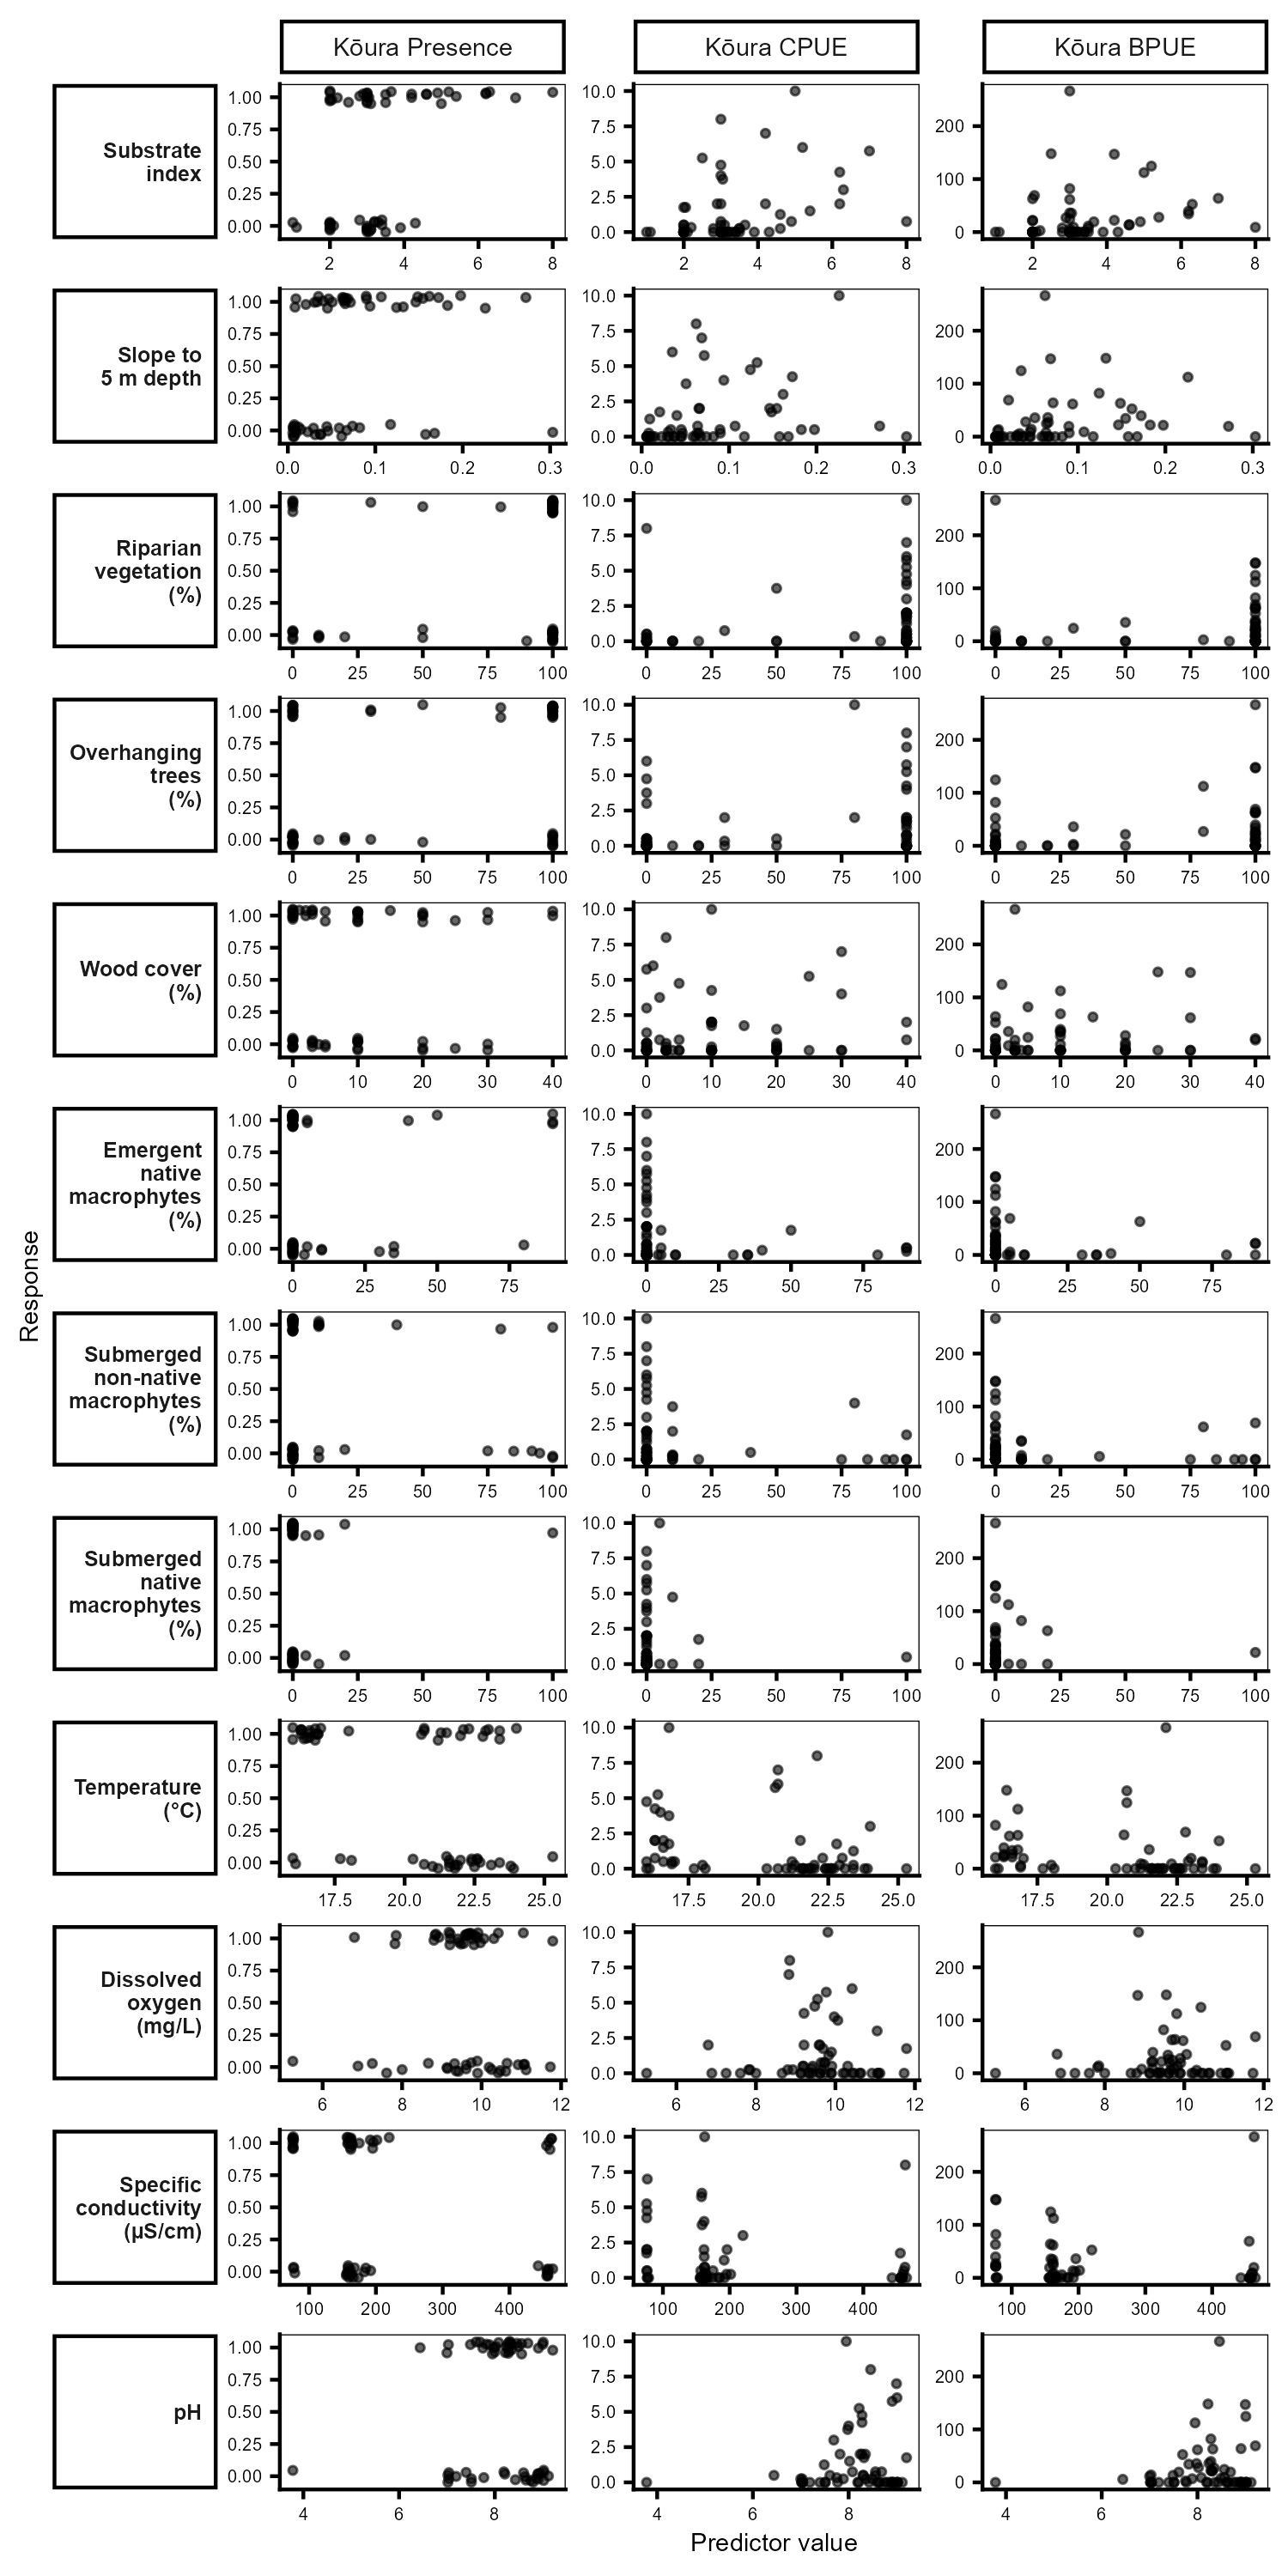
\includegraphics[width=0.65\linewidth,height=\textheight,keepaspectratio]{outputs/fig-raw-data-all-predictors.png}

}

\caption{\label{fig-raw-data-all-predictors}Raw relationships between
all environmental predictors examined and kōura occurrence, CPUE, and
BPUE across all 60 surveyed littoral sites. Each panel shows observed
values at individual sites (n = 60 for occurrence; n = 33 for CPUE and
BPUE). Points are jittered slightly for occurrence data to reduce
overplotting. Predictors highlighted in bold were retained in final GAM
models.}

\end{figure}%

\begingroup\fontsize{8}{10}\selectfont

\begin{longtable}[t]{lllrrrrrrr}

\caption{\label{tbl-an-env-fish-summary}Distribution of environmental
and biotic variables measured at littoral sampling sites across five Te
Arawa lakes in the Rotorua region of Aotearoa New Zealand.}

\tabularnewline

\toprule
Lake & Variable & Unit & n & Mean & Median & Min & Max & CI low & CI high\\
\midrule
\endfirsthead
\multicolumn{10}{@{}l}{\textit{(continued)}}\\
\toprule
Lake & Variable & Unit & n & Mean & Median & Min & Max & CI low & CI high\\
\midrule
\endhead

\endfoot
\bottomrule
\endlastfoot
\cellcolor{gray!8}{Rotorua} & \cellcolor{gray!8}{Substrate index} & \cellcolor{gray!8}{} & \cellcolor{gray!8}{12} & \cellcolor{gray!8}{3.66} & \cellcolor{gray!8}{3.30} & \cellcolor{gray!8}{2.80} & \cellcolor{gray!8}{6.30} & \cellcolor{gray!8}{3.01} & \cellcolor{gray!8}{4.31}\\
Rotoiti & Substrate index &  & 12 & 3.92 & 3.20 & 2.00 & 8.00 & 2.73 & 5.11\\
\cellcolor{gray!8}{Rotoehu} & \cellcolor{gray!8}{Substrate index} & \cellcolor{gray!8}{} & \cellcolor{gray!8}{12} & \cellcolor{gray!8}{2.77} & \cellcolor{gray!8}{2.45} & \cellcolor{gray!8}{2.00} & \cellcolor{gray!8}{4.90} & \cellcolor{gray!8}{2.15} & \cellcolor{gray!8}{3.39}\\
Rotomā & Substrate index &  & 12 & 3.50 & 3.02 & 2.00 & 6.20 & 2.64 & 4.36\\
\cellcolor{gray!8}{Ōkāreka} & \cellcolor{gray!8}{Substrate index} & \cellcolor{gray!8}{} & \cellcolor{gray!8}{12} & \cellcolor{gray!8}{2.86} & \cellcolor{gray!8}{2.70} & \cellcolor{gray!8}{1.00} & \cellcolor{gray!8}{6.20} & \cellcolor{gray!8}{1.92} & \cellcolor{gray!8}{3.79}\\
\addlinespace
All lakes & Substrate index &  & 60 & 3.34 & 3.00 & 1.00 & 8.00 & 2.98 & 3.71\\
\cellcolor{gray!8}{Rotorua} & \cellcolor{gray!8}{Slope 5m} & \cellcolor{gray!8}{} & \cellcolor{gray!8}{12} & \cellcolor{gray!8}{0.02} & \cellcolor{gray!8}{0.01} & \cellcolor{gray!8}{0.01} & \cellcolor{gray!8}{0.16} & \cellcolor{gray!8}{0.00} & \cellcolor{gray!8}{0.05}\\
Rotoiti & Slope 5m &  & 12 & 0.09 & 0.07 & 0.04 & 0.30 & 0.04 & 0.14\\
\cellcolor{gray!8}{Rotoehu} & \cellcolor{gray!8}{Slope 5m} & \cellcolor{gray!8}{} & \cellcolor{gray!8}{12} & \cellcolor{gray!8}{0.08} & \cellcolor{gray!8}{0.06} & \cellcolor{gray!8}{0.02} & \cellcolor{gray!8}{0.27} & \cellcolor{gray!8}{0.03} & \cellcolor{gray!8}{0.12}\\
Rotomā & Slope 5m &  & 12 & 0.07 & 0.06 & 0.01 & 0.23 & 0.03 & 0.11\\
\addlinespace
\cellcolor{gray!8}{Ōkāreka} & \cellcolor{gray!8}{Slope 5m} & \cellcolor{gray!8}{} & \cellcolor{gray!8}{12} & \cellcolor{gray!8}{0.11} & \cellcolor{gray!8}{0.13} & \cellcolor{gray!8}{0.01} & \cellcolor{gray!8}{0.20} & \cellcolor{gray!8}{0.07} & \cellcolor{gray!8}{0.15}\\
All lakes & Slope 5m &  & 60 & 0.08 & 0.06 & 0.01 & 0.30 & 0.06 & 0.09\\
\cellcolor{gray!8}{Rotorua} & \cellcolor{gray!8}{Riparian vegetation} & \cellcolor{gray!8}{\%} & \cellcolor{gray!8}{12} & \cellcolor{gray!8}{67.50} & \cellcolor{gray!8}{100.00} & \cellcolor{gray!8}{0.00} & \cellcolor{gray!8}{100.00} & \cellcolor{gray!8}{40.12} & \cellcolor{gray!8}{94.88}\\
Rotoiti & Riparian vegetation & \% & 12 & 92.50 & 100.00 & 20.00 & 100.00 & 77.88 & 107.12\\
\cellcolor{gray!8}{Rotoehu} & \cellcolor{gray!8}{Riparian vegetation} & \cellcolor{gray!8}{\%} & \cellcolor{gray!8}{12} & \cellcolor{gray!8}{67.50} & \cellcolor{gray!8}{100.00} & \cellcolor{gray!8}{0.00} & \cellcolor{gray!8}{100.00} & \cellcolor{gray!8}{36.95} & \cellcolor{gray!8}{98.05}\\
\addlinespace
Rotomā & Riparian vegetation & \% & 12 & 63.33 & 90.00 & 0.00 & 100.00 & 35.13 & 91.53\\
\cellcolor{gray!8}{Ōkāreka} & \cellcolor{gray!8}{Riparian vegetation} & \cellcolor{gray!8}{\%} & \cellcolor{gray!8}{12} & \cellcolor{gray!8}{75.83} & \cellcolor{gray!8}{100.00} & \cellcolor{gray!8}{0.00} & \cellcolor{gray!8}{100.00} & \cellcolor{gray!8}{48.01} & \cellcolor{gray!8}{103.66}\\
All lakes & Riparian vegetation & \% & 60 & 73.33 & 100.00 & 0.00 & 100.00 & 62.65 & 84.02\\
\cellcolor{gray!8}{Rotorua} & \cellcolor{gray!8}{Overhanging trees} & \cellcolor{gray!8}{\%} & \cellcolor{gray!8}{12} & \cellcolor{gray!8}{46.67} & \cellcolor{gray!8}{30.00} & \cellcolor{gray!8}{0.00} & \cellcolor{gray!8}{100.00} & \cellcolor{gray!8}{15.50} & \cellcolor{gray!8}{77.83}\\
Rotoiti & Overhanging trees & \% & 12 & 54.17 & 65.00 & 0.00 & 100.00 & 23.22 & 85.11\\
\addlinespace
\cellcolor{gray!8}{Rotoehu} & \cellcolor{gray!8}{Overhanging trees} & \cellcolor{gray!8}{\%} & \cellcolor{gray!8}{12} & \cellcolor{gray!8}{35.83} & \cellcolor{gray!8}{0.00} & \cellcolor{gray!8}{0.00} & \cellcolor{gray!8}{100.00} & \cellcolor{gray!8}{5.25} & \cellcolor{gray!8}{66.42}\\
Rotomā & Overhanging trees & \% & 12 & 52.50 & 55.00 & 0.00 & 100.00 & 22.44 & 82.56\\
\cellcolor{gray!8}{Ōkāreka} & \cellcolor{gray!8}{Overhanging trees} & \cellcolor{gray!8}{\%} & \cellcolor{gray!8}{12} & \cellcolor{gray!8}{52.50} & \cellcolor{gray!8}{65.00} & \cellcolor{gray!8}{0.00} & \cellcolor{gray!8}{100.00} & \cellcolor{gray!8}{21.71} & \cellcolor{gray!8}{83.29}\\
All lakes & Overhanging trees & \% & 60 & 48.33 & 30.00 & 0.00 & 100.00 & 36.15 & 60.52\\
\cellcolor{gray!8}{Rotorua} & \cellcolor{gray!8}{Wood cover} & \cellcolor{gray!8}{\%} & \cellcolor{gray!8}{12} & \cellcolor{gray!8}{8.33} & \cellcolor{gray!8}{3.50} & \cellcolor{gray!8}{0.00} & \cellcolor{gray!8}{30.00} & \cellcolor{gray!8}{1.98} & \cellcolor{gray!8}{14.69}\\
\addlinespace
Rotoiti & Wood cover & \% & 12 & 4.25 & 1.50 & 0.00 & 20.00 & 0.31 & 8.19\\
\cellcolor{gray!8}{Rotoehu} & \cellcolor{gray!8}{Wood cover} & \cellcolor{gray!8}{\%} & \cellcolor{gray!8}{12} & \cellcolor{gray!8}{14.92} & \cellcolor{gray!8}{10.00} & \cellcolor{gray!8}{3.00} & \cellcolor{gray!8}{40.00} & \cellcolor{gray!8}{7.24} & \cellcolor{gray!8}{22.60}\\
Rotomā & Wood cover & \% & 12 & 10.00 & 10.00 & 0.00 & 30.00 & 4.13 & 15.87\\
\cellcolor{gray!8}{Ōkāreka} & \cellcolor{gray!8}{Wood cover} & \cellcolor{gray!8}{\%} & \cellcolor{gray!8}{12} & \cellcolor{gray!8}{11.25} & \cellcolor{gray!8}{7.50} & \cellcolor{gray!8}{0.00} & \cellcolor{gray!8}{40.00} & \cellcolor{gray!8}{2.56} & \cellcolor{gray!8}{19.94}\\
All lakes & Wood cover & \% & 60 & 9.75 & 5.00 & 0.00 & 40.00 & 6.96 & 12.54\\
\addlinespace
\cellcolor{gray!8}{Rotorua} & \cellcolor{gray!8}{Emergent macrophytes} & \cellcolor{gray!8}{\%} & \cellcolor{gray!8}{12} & \cellcolor{gray!8}{0.00} & \cellcolor{gray!8}{0.00} & \cellcolor{gray!8}{0.00} & \cellcolor{gray!8}{0.00} & \cellcolor{gray!8}{0.00} & \cellcolor{gray!8}{0.00}\\
Rotoiti & Emergent macrophytes & \% & 12 & 9.50 & 0.00 & 0.00 & 100.00 & -8.71 & 27.71\\
\cellcolor{gray!8}{Rotoehu} & \cellcolor{gray!8}{Emergent macrophytes} & \cellcolor{gray!8}{\%} & \cellcolor{gray!8}{12} & \cellcolor{gray!8}{8.75} & \cellcolor{gray!8}{0.00} & \cellcolor{gray!8}{0.00} & \cellcolor{gray!8}{35.00} & \cellcolor{gray!8}{-0.74} & \cellcolor{gray!8}{18.24}\\
Rotomā & Emergent macrophytes & \% & 12 & 10.83 & 0.00 & 0.00 & 80.00 & -4.78 & 26.45\\
\cellcolor{gray!8}{Ōkāreka} & \cellcolor{gray!8}{Emergent macrophytes} & \cellcolor{gray!8}{\%} & \cellcolor{gray!8}{12} & \cellcolor{gray!8}{22.50} & \cellcolor{gray!8}{0.00} & \cellcolor{gray!8}{0.00} & \cellcolor{gray!8}{90.00} & \cellcolor{gray!8}{-0.35} & \cellcolor{gray!8}{45.35}\\
\addlinespace
All lakes & Emergent macrophytes & \% & 60 & 10.32 & 0.00 & 0.00 & 100.00 & 3.98 & 16.65\\
\cellcolor{gray!8}{Rotorua} & \cellcolor{gray!8}{Submerged macrophytes} & \cellcolor{gray!8}{\%} & \cellcolor{gray!8}{12} & \cellcolor{gray!8}{0.83} & \cellcolor{gray!8}{0.00} & \cellcolor{gray!8}{0.00} & \cellcolor{gray!8}{10.00} & \cellcolor{gray!8}{-1.00} & \cellcolor{gray!8}{2.67}\\
Rotoiti & Submerged macrophytes & \% & 12 & 0.83 & 0.00 & 0.00 & 10.00 & -1.00 & 2.67\\
\cellcolor{gray!8}{Rotoehu} & \cellcolor{gray!8}{Submerged macrophytes} & \cellcolor{gray!8}{\%} & \cellcolor{gray!8}{12} & \cellcolor{gray!8}{51.42} & \cellcolor{gray!8}{52.50} & \cellcolor{gray!8}{0.00} & \cellcolor{gray!8}{100.00} & \cellcolor{gray!8}{20.51} & \cellcolor{gray!8}{82.33}\\
Rotomā & Submerged macrophytes & \% & 12 & 21.67 & 10.00 & 0.00 & 85.00 & 2.21 & 41.12\\
\addlinespace
\cellcolor{gray!8}{Ōkāreka} & \cellcolor{gray!8}{Submerged macrophytes} & \cellcolor{gray!8}{\%} & \cellcolor{gray!8}{12} & \cellcolor{gray!8}{10.83} & \cellcolor{gray!8}{0.00} & \cellcolor{gray!8}{0.00} & \cellcolor{gray!8}{100.00} & \cellcolor{gray!8}{-7.43} & \cellcolor{gray!8}{29.10}\\
All lakes & Submerged macrophytes & \% & 60 & 17.12 & 0.00 & 0.00 & 100.00 & 8.42 & 25.81\\
\cellcolor{gray!8}{Rotorua} & \cellcolor{gray!8}{Temperature} & \cellcolor{gray!8}{Degree C} & \cellcolor{gray!8}{12} & \cellcolor{gray!8}{23.15} & \cellcolor{gray!8}{23.25} & \cellcolor{gray!8}{21.80} & \cellcolor{gray!8}{25.30} & \cellcolor{gray!8}{22.52} & \cellcolor{gray!8}{23.78}\\
Rotoiti & Temperature & Degree C & 12 & 21.62 & 21.50 & 20.60 & 23.80 & 21.03 & 22.22\\
\cellcolor{gray!8}{Rotoehu} & \cellcolor{gray!8}{Temperature} & \cellcolor{gray!8}{Degree C} & \cellcolor{gray!8}{12} & \cellcolor{gray!8}{22.11} & \cellcolor{gray!8}{22.05} & \cellcolor{gray!8}{21.20} & \cellcolor{gray!8}{23.00} & \cellcolor{gray!8}{21.72} & \cellcolor{gray!8}{22.49}\\
\addlinespace
Rotomā & Temperature & Degree C & 12 & 17.02 & 16.85 & 16.30 & 18.10 & 16.64 & 17.39\\
\cellcolor{gray!8}{Ōkāreka} & \cellcolor{gray!8}{Temperature} & \cellcolor{gray!8}{Degree C} & \cellcolor{gray!8}{12} & \cellcolor{gray!8}{16.98} & \cellcolor{gray!8}{16.30} & \cellcolor{gray!8}{16.00} & \cellcolor{gray!8}{20.70} & \cellcolor{gray!8}{15.93} & \cellcolor{gray!8}{18.04}\\
All lakes & Temperature & Degree C & 60 & 20.18 & 21.25 & 16.00 & 25.30 & 19.44 & 20.91\\
\cellcolor{gray!8}{Rotorua} & \cellcolor{gray!8}{Dissolved oxygen} & \cellcolor{gray!8}{mg/l} & \cellcolor{gray!8}{12} & \cellcolor{gray!8}{8.49} & \cellcolor{gray!8}{7.92} & \cellcolor{gray!8}{5.25} & \cellcolor{gray!8}{11.05} & \cellcolor{gray!8}{7.39} & \cellcolor{gray!8}{9.59}\\
Rotoiti & Dissolved oxygen & mg/l & 12 & 9.59 & 9.76 & 6.80 & 10.64 & 8.92 & 10.25\\
\addlinespace
\cellcolor{gray!8}{Rotoehu} & \cellcolor{gray!8}{Dissolved oxygen} & \cellcolor{gray!8}{mg/l} & \cellcolor{gray!8}{12} & \cellcolor{gray!8}{10.36} & \cellcolor{gray!8}{10.77} & \cellcolor{gray!8}{8.85} & \cellcolor{gray!8}{11.79} & \cellcolor{gray!8}{9.67} & \cellcolor{gray!8}{11.05}\\
Rotomā & Dissolved oxygen & mg/l & 12 & 9.72 & 9.76 & 8.66 & 10.31 & 9.45 & 9.98\\
\cellcolor{gray!8}{Ōkāreka} & \cellcolor{gray!8}{Dissolved oxygen} & \cellcolor{gray!8}{mg/l} & \cellcolor{gray!8}{12} & \cellcolor{gray!8}{9.37} & \cellcolor{gray!8}{9.38} & \cellcolor{gray!8}{8.83} & \cellcolor{gray!8}{9.74} & \cellcolor{gray!8}{9.20} & \cellcolor{gray!8}{9.53}\\
All lakes & Dissolved oxygen & mg/l & 60 & 9.50 & 9.62 & 5.25 & 11.79 & 9.20 & 9.81\\
\cellcolor{gray!8}{Rotorua} & \cellcolor{gray!8}{Specific conductivity} & \cellcolor{gray!8}{µS/cm} & \cellcolor{gray!8}{12} & \cellcolor{gray!8}{205.36} & \cellcolor{gray!8}{188.27} & \cellcolor{gray!8}{156.20} & \cellcolor{gray!8}{443.01} & \cellcolor{gray!8}{156.39} & \cellcolor{gray!8}{254.33}\\
\addlinespace
Rotoiti & Specific conductivity & µS/cm & 12 & 163.11 & 158.70 & 155.79 & 196.01 & 156.22 & 170.00\\
\cellcolor{gray!8}{Rotoehu} & \cellcolor{gray!8}{Specific conductivity} & \cellcolor{gray!8}{µS/cm} & \cellcolor{gray!8}{12} & \cellcolor{gray!8}{458.89} & \cellcolor{gray!8}{458.22} & \cellcolor{gray!8}{455.44} & \cellcolor{gray!8}{464.72} & \cellcolor{gray!8}{456.91} & \cellcolor{gray!8}{460.87}\\
Rotomā & Specific conductivity & µS/cm & 12 & 162.90 & 161.79 & 156.73 & 174.96 & 159.94 & 165.85\\
\cellcolor{gray!8}{Ōkāreka} & \cellcolor{gray!8}{Specific conductivity} & \cellcolor{gray!8}{µS/cm} & \cellcolor{gray!8}{12} & \cellcolor{gray!8}{76.34} & \cellcolor{gray!8}{76.15} & \cellcolor{gray!8}{75.62} & \cellcolor{gray!8}{78.59} & \cellcolor{gray!8}{75.82} & \cellcolor{gray!8}{76.86}\\
All lakes & Specific conductivity & µS/cm & 60 & 213.32 & 162.55 & 75.62 & 464.72 & 178.41 & 248.23\\
\addlinespace
\cellcolor{gray!8}{Rotorua} & \cellcolor{gray!8}{pH} & \cellcolor{gray!8}{} & \cellcolor{gray!8}{12} & \cellcolor{gray!8}{6.94} & \cellcolor{gray!8}{7.04} & \cellcolor{gray!8}{3.78} & \cellcolor{gray!8}{7.69} & \cellcolor{gray!8}{6.29} & \cellcolor{gray!8}{7.60}\\
Rotoiti & pH &  & 12 & 8.67 & 8.72 & 8.08 & 9.02 & 8.46 & 8.87\\
\cellcolor{gray!8}{Rotoehu} & \cellcolor{gray!8}{pH} & \cellcolor{gray!8}{} & \cellcolor{gray!8}{12} & \cellcolor{gray!8}{8.83} & \cellcolor{gray!8}{8.90} & \cellcolor{gray!8}{8.46} & \cellcolor{gray!8}{9.21} & \cellcolor{gray!8}{8.68} & \cellcolor{gray!8}{8.99}\\
Rotomā & pH &  & 12 & 7.80 & 7.92 & 6.44 & 8.56 & 7.47 & 8.13\\
\cellcolor{gray!8}{Ōkāreka} & \cellcolor{gray!8}{pH} & \cellcolor{gray!8}{} & \cellcolor{gray!8}{12} & \cellcolor{gray!8}{8.32} & \cellcolor{gray!8}{8.29} & \cellcolor{gray!8}{7.77} & \cellcolor{gray!8}{9.00} & \cellcolor{gray!8}{8.15} & \cellcolor{gray!8}{8.50}\\
\addlinespace
All lakes & pH &  & 60 & 8.11 & 8.28 & 3.78 & 9.21 & 7.89 & 8.34\\
\cellcolor{gray!8}{Rotorua} & \cellcolor{gray!8}{Presence Catfish} & \cellcolor{gray!8}{} & \cellcolor{gray!8}{12} & \cellcolor{gray!8}{0.08} & \cellcolor{gray!8}{0.00} & \cellcolor{gray!8}{0.00} & \cellcolor{gray!8}{1.00} & \cellcolor{gray!8}{0.00} & \cellcolor{gray!8}{0.38}\\
Rotoiti & Presence Catfish &  & 12 & 0.42 & 0.00 & 0.00 & 1.00 & 0.15 & 0.72\\
\cellcolor{gray!8}{Rotoehu} & \cellcolor{gray!8}{Presence Catfish} & \cellcolor{gray!8}{} & \cellcolor{gray!8}{12} & \cellcolor{gray!8}{0.00} & \cellcolor{gray!8}{0.00} & \cellcolor{gray!8}{0.00} & \cellcolor{gray!8}{0.00} & \cellcolor{gray!8}{0.00} & \cellcolor{gray!8}{0.26}\\
Rotomā & Presence Catfish &  & 12 & 0.00 & 0.00 & 0.00 & 0.00 & 0.00 & 0.26\\
\addlinespace
\cellcolor{gray!8}{Ōkāreka} & \cellcolor{gray!8}{Presence Catfish} & \cellcolor{gray!8}{} & \cellcolor{gray!8}{12} & \cellcolor{gray!8}{0.00} & \cellcolor{gray!8}{0.00} & \cellcolor{gray!8}{0.00} & \cellcolor{gray!8}{0.00} & \cellcolor{gray!8}{0.00} & \cellcolor{gray!8}{0.26}\\
All lakes & Presence Catfish &  & 60 & 0.10 & 0.00 & 0.00 & 1.00 & 0.04 & 0.21\\
\cellcolor{gray!8}{Rotorua} & \cellcolor{gray!8}{Presence Eel} & \cellcolor{gray!8}{} & \cellcolor{gray!8}{12} & \cellcolor{gray!8}{0.33} & \cellcolor{gray!8}{0.00} & \cellcolor{gray!8}{0.00} & \cellcolor{gray!8}{1.00} & \cellcolor{gray!8}{0.10} & \cellcolor{gray!8}{0.65}\\
Rotoiti & Presence Eel &  & 12 & 0.08 & 0.00 & 0.00 & 1.00 & 0.00 & 0.38\\
\cellcolor{gray!8}{Rotoehu} & \cellcolor{gray!8}{Presence Eel} & \cellcolor{gray!8}{} & \cellcolor{gray!8}{12} & \cellcolor{gray!8}{0.00} & \cellcolor{gray!8}{0.00} & \cellcolor{gray!8}{0.00} & \cellcolor{gray!8}{0.00} & \cellcolor{gray!8}{0.00} & \cellcolor{gray!8}{0.26}\\
\addlinespace
Rotomā & Presence Eel &  & 12 & 0.25 & 0.00 & 0.00 & 1.00 & 0.05 & 0.57\\
\cellcolor{gray!8}{Ōkāreka} & \cellcolor{gray!8}{Presence Eel} & \cellcolor{gray!8}{} & \cellcolor{gray!8}{12} & \cellcolor{gray!8}{0.00} & \cellcolor{gray!8}{0.00} & \cellcolor{gray!8}{0.00} & \cellcolor{gray!8}{0.00} & \cellcolor{gray!8}{0.00} & \cellcolor{gray!8}{0.26}\\
All lakes & Presence Eel &  & 60 & 0.13 & 0.00 & 0.00 & 1.00 & 0.06 & 0.25\\
\cellcolor{gray!8}{Rotorua} & \cellcolor{gray!8}{Presence Goldfish} & \cellcolor{gray!8}{} & \cellcolor{gray!8}{12} & \cellcolor{gray!8}{0.08} & \cellcolor{gray!8}{0.00} & \cellcolor{gray!8}{0.00} & \cellcolor{gray!8}{1.00} & \cellcolor{gray!8}{0.00} & \cellcolor{gray!8}{0.38}\\
Rotoiti & Presence Goldfish &  & 12 & 0.67 & 1.00 & 0.00 & 1.00 & 0.35 & 0.90\\
\addlinespace
\cellcolor{gray!8}{Rotoehu} & \cellcolor{gray!8}{Presence Goldfish} & \cellcolor{gray!8}{} & \cellcolor{gray!8}{12} & \cellcolor{gray!8}{1.00} & \cellcolor{gray!8}{1.00} & \cellcolor{gray!8}{1.00} & \cellcolor{gray!8}{1.00} & \cellcolor{gray!8}{0.74} & \cellcolor{gray!8}{1.00}\\
Rotomā & Presence Goldfish &  & 12 & 0.50 & 0.50 & 0.00 & 1.00 & 0.21 & 0.79\\
\cellcolor{gray!8}{Ōkāreka} & \cellcolor{gray!8}{Presence Goldfish} & \cellcolor{gray!8}{} & \cellcolor{gray!8}{12} & \cellcolor{gray!8}{0.25} & \cellcolor{gray!8}{0.00} & \cellcolor{gray!8}{0.00} & \cellcolor{gray!8}{1.00} & \cellcolor{gray!8}{0.05} & \cellcolor{gray!8}{0.57}\\
All lakes & Presence Goldfish &  & 60 & 0.50 & 0.50 & 0.00 & 1.00 & 0.37 & 0.63\\
\cellcolor{gray!8}{Rotorua} & \cellcolor{gray!8}{Presence Common smelt} & \cellcolor{gray!8}{} & \cellcolor{gray!8}{12} & \cellcolor{gray!8}{0.25} & \cellcolor{gray!8}{0.00} & \cellcolor{gray!8}{0.00} & \cellcolor{gray!8}{1.00} & \cellcolor{gray!8}{0.05} & \cellcolor{gray!8}{0.57}\\
\addlinespace
Rotoiti & Presence Common smelt &  & 12 & 0.67 & 1.00 & 0.00 & 1.00 & 0.35 & 0.90\\
\cellcolor{gray!8}{Rotoehu} & \cellcolor{gray!8}{Presence Common smelt} & \cellcolor{gray!8}{} & \cellcolor{gray!8}{12} & \cellcolor{gray!8}{0.50} & \cellcolor{gray!8}{0.50} & \cellcolor{gray!8}{0.00} & \cellcolor{gray!8}{1.00} & \cellcolor{gray!8}{0.21} & \cellcolor{gray!8}{0.79}\\
Rotomā & Presence Common smelt &  & 12 & 0.42 & 0.00 & 0.00 & 1.00 & 0.15 & 0.72\\
\cellcolor{gray!8}{Ōkāreka} & \cellcolor{gray!8}{Presence Common smelt} & \cellcolor{gray!8}{} & \cellcolor{gray!8}{12} & \cellcolor{gray!8}{0.58} & \cellcolor{gray!8}{1.00} & \cellcolor{gray!8}{0.00} & \cellcolor{gray!8}{1.00} & \cellcolor{gray!8}{0.28} & \cellcolor{gray!8}{0.85}\\
All lakes & Presence Common smelt &  & 60 & 0.48 & 0.00 & 0.00 & 1.00 & 0.35 & 0.62\\
\addlinespace
\cellcolor{gray!8}{Rotorua} & \cellcolor{gray!8}{Presence Kōaro} & \cellcolor{gray!8}{} & \cellcolor{gray!8}{12} & \cellcolor{gray!8}{0.00} & \cellcolor{gray!8}{0.00} & \cellcolor{gray!8}{0.00} & \cellcolor{gray!8}{0.00} & \cellcolor{gray!8}{0.00} & \cellcolor{gray!8}{0.26}\\
Rotoiti & Presence Kōaro &  & 12 & 0.00 & 0.00 & 0.00 & 0.00 & 0.00 & 0.26\\
\cellcolor{gray!8}{Rotoehu} & \cellcolor{gray!8}{Presence Kōaro} & \cellcolor{gray!8}{} & \cellcolor{gray!8}{12} & \cellcolor{gray!8}{0.00} & \cellcolor{gray!8}{0.00} & \cellcolor{gray!8}{0.00} & \cellcolor{gray!8}{0.00} & \cellcolor{gray!8}{0.00} & \cellcolor{gray!8}{0.26}\\
Rotomā & Presence Kōaro &  & 12 & 0.00 & 0.00 & 0.00 & 0.00 & 0.00 & 0.26\\
\cellcolor{gray!8}{Ōkāreka} & \cellcolor{gray!8}{Presence Kōaro} & \cellcolor{gray!8}{} & \cellcolor{gray!8}{12} & \cellcolor{gray!8}{0.67} & \cellcolor{gray!8}{1.00} & \cellcolor{gray!8}{0.00} & \cellcolor{gray!8}{1.00} & \cellcolor{gray!8}{0.35} & \cellcolor{gray!8}{0.90}\\
\addlinespace
All lakes & Presence Kōaro &  & 60 & 0.13 & 0.00 & 0.00 & 1.00 & 0.06 & 0.25\\
\cellcolor{gray!8}{Rotorua} & \cellcolor{gray!8}{Presence Trout} & \cellcolor{gray!8}{} & \cellcolor{gray!8}{12} & \cellcolor{gray!8}{0.17} & \cellcolor{gray!8}{0.00} & \cellcolor{gray!8}{0.00} & \cellcolor{gray!8}{1.00} & \cellcolor{gray!8}{0.02} & \cellcolor{gray!8}{0.48}\\
Rotoiti & Presence Trout &  & 12 & 0.17 & 0.00 & 0.00 & 1.00 & 0.02 & 0.48\\
\cellcolor{gray!8}{Rotoehu} & \cellcolor{gray!8}{Presence Trout} & \cellcolor{gray!8}{} & \cellcolor{gray!8}{12} & \cellcolor{gray!8}{0.00} & \cellcolor{gray!8}{0.00} & \cellcolor{gray!8}{0.00} & \cellcolor{gray!8}{0.00} & \cellcolor{gray!8}{0.00} & \cellcolor{gray!8}{0.26}\\
Rotomā & Presence Trout &  & 12 & 0.00 & 0.00 & 0.00 & 0.00 & 0.00 & 0.26\\
\addlinespace
\cellcolor{gray!8}{Ōkāreka} & \cellcolor{gray!8}{Presence Trout} & \cellcolor{gray!8}{} & \cellcolor{gray!8}{12} & \cellcolor{gray!8}{0.17} & \cellcolor{gray!8}{0.00} & \cellcolor{gray!8}{0.00} & \cellcolor{gray!8}{1.00} & \cellcolor{gray!8}{0.02} & \cellcolor{gray!8}{0.48}\\
All lakes & Presence Trout &  & 60 & 0.10 & 0.00 & 0.00 & 1.00 & 0.04 & 0.21\\*

\end{longtable}

\endgroup{}

\clearpage
\setcounter{table}{0}
\setcounter{figure}{0}

\section*{Chapter 5 --- Supplementary
information}\label{chapter-5-supplementary-information}
\addcontentsline{toc}{section}{Chapter 5 --- Supplementary information}

\begin{figure}

\centering{

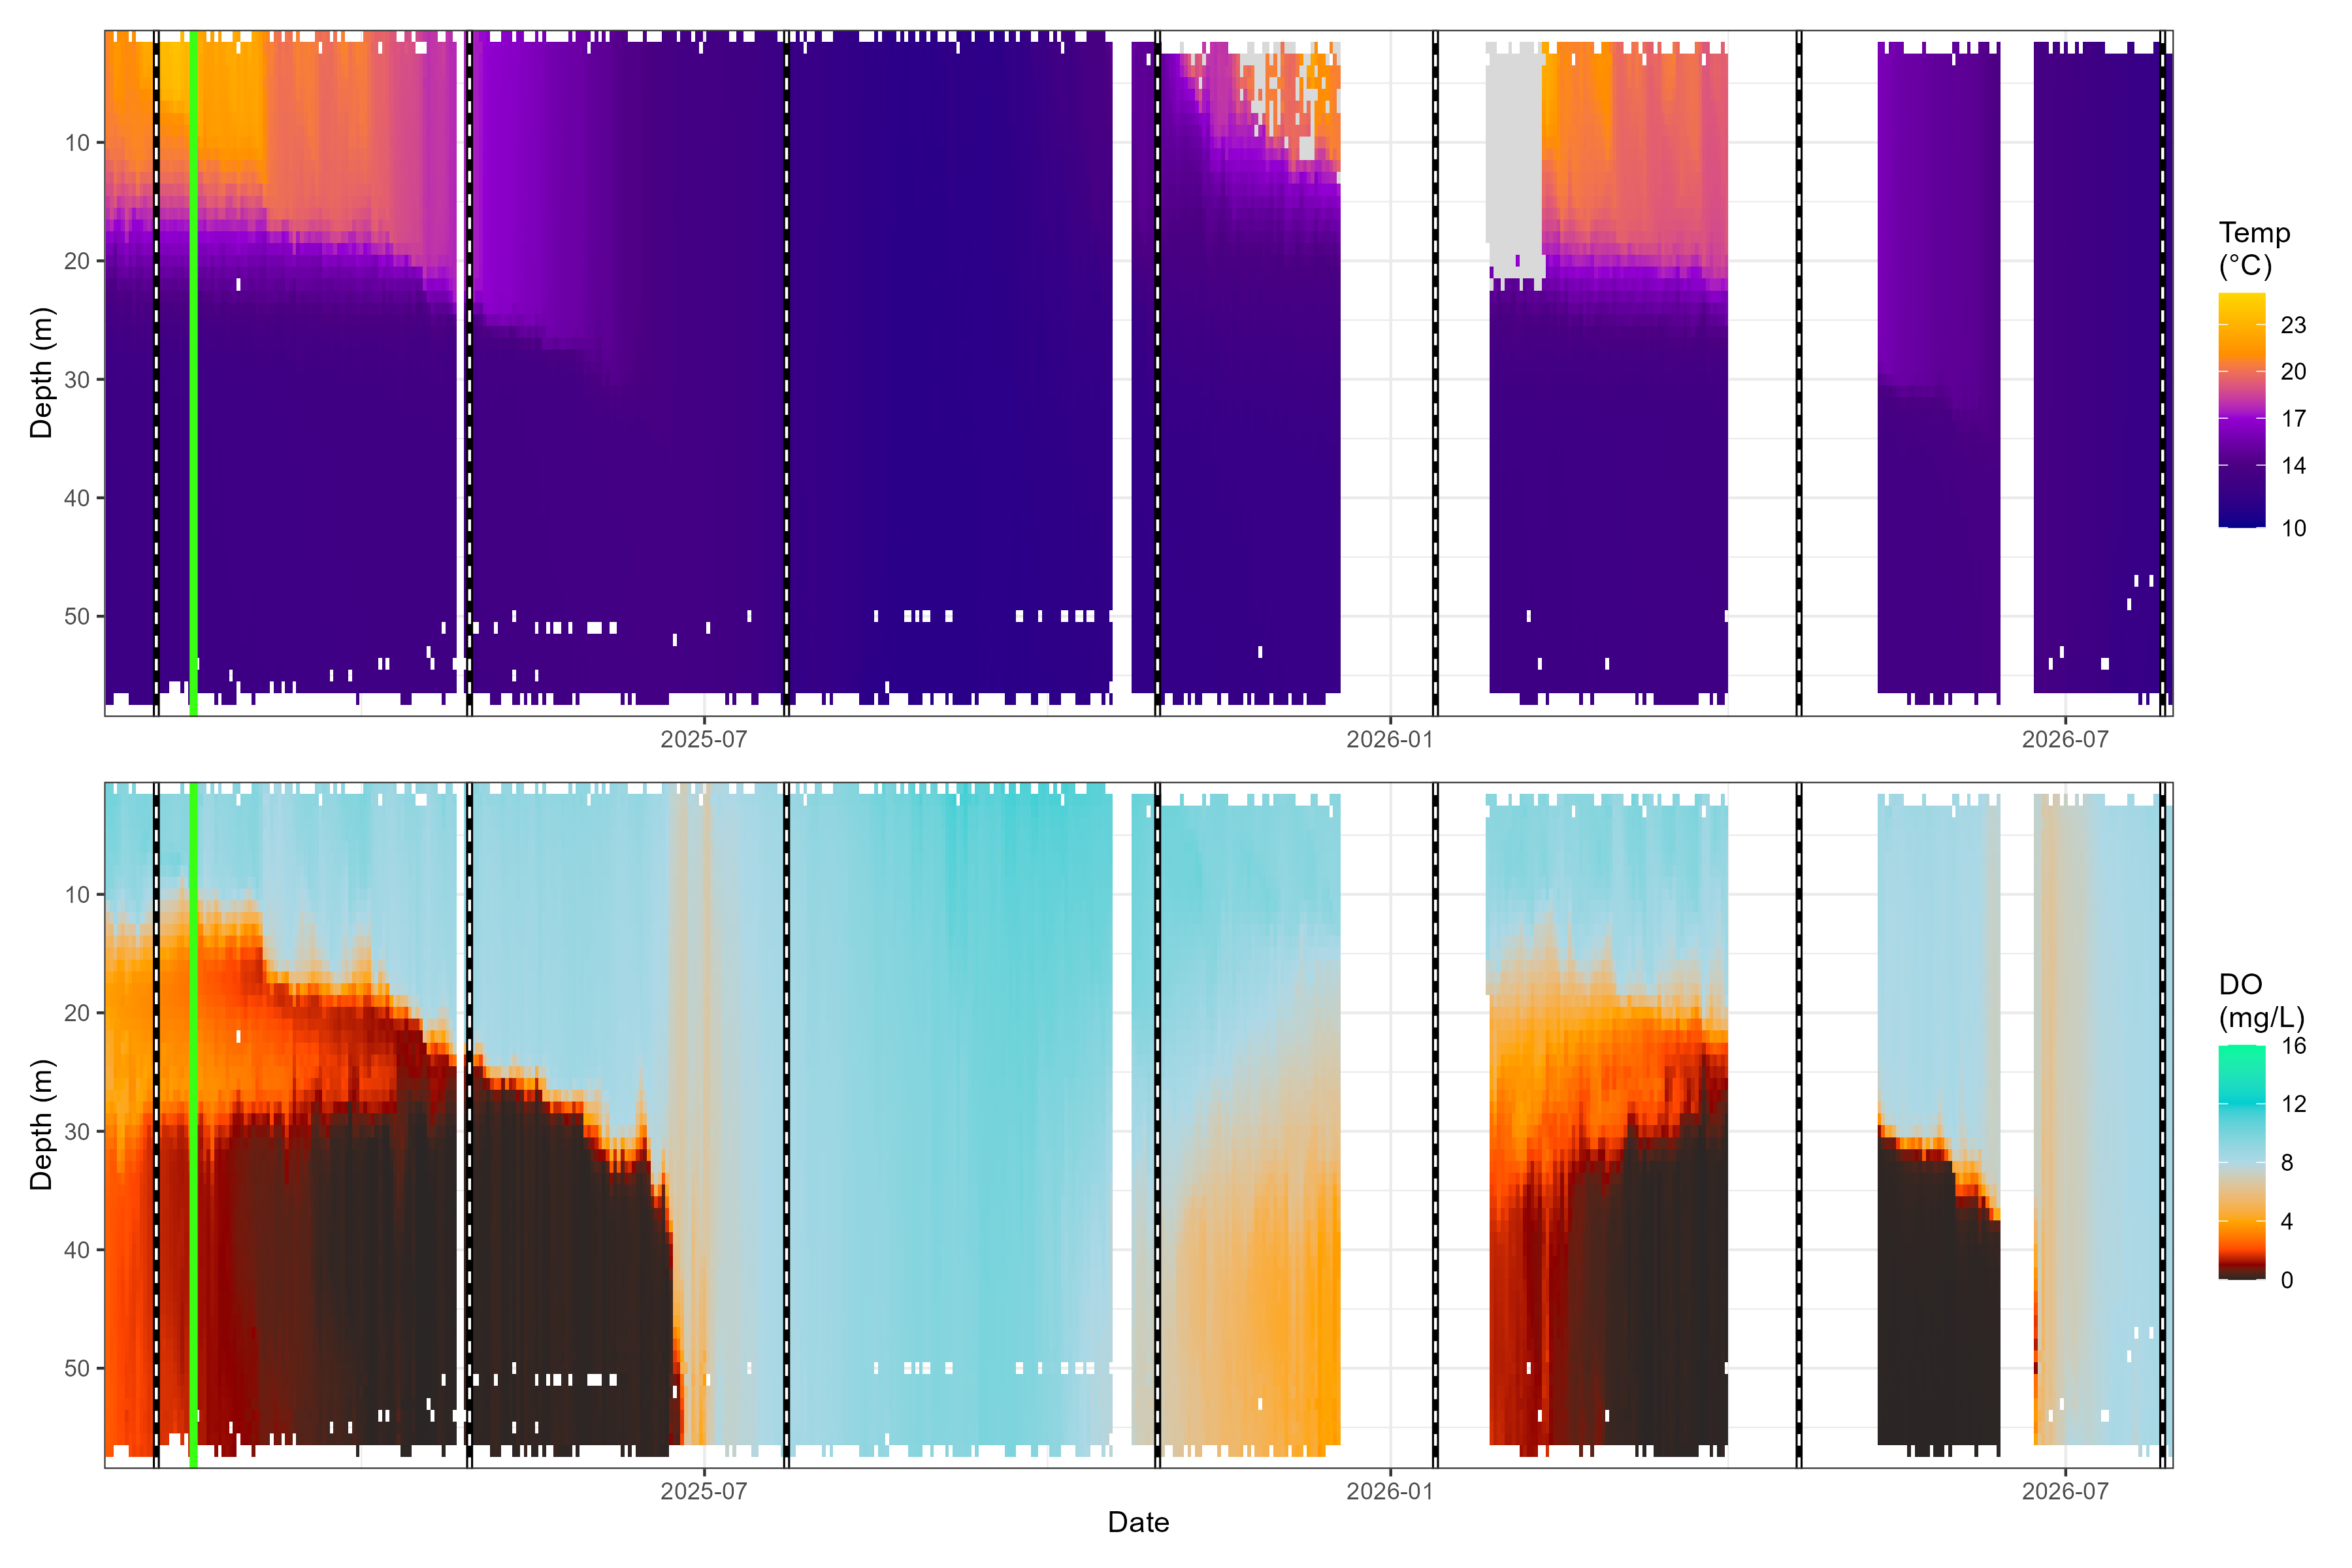
\includegraphics[width=0.8\linewidth,height=\textheight,keepaspectratio]{outputs/fig-lake-conditions.png}

}

\caption{\label{fig-lake-conditions}Depth-resolved water temperature
(°C, top) and dissolved oxygen (mg/L, bottom) in Lake Rotoiti throughout
the study period (February 2025 -- July 2026). Data derived from the
LimnoTrack continuous monitoring buoy (Moore and McBride 2026). Vertical
green line marks stone pile deployment; dashed vertical lines mark
seasonal monitoring rounds. Warm colours in the DO panel (orange--black)
indicate hypoxic and anoxic conditions (\textless{} 5 mg/L),
demonstrating the pronounced summer stratification that compresses
oxygenated habitat into the shallow littoral zone.}

\end{figure}%

\begin{figure}

\centering{

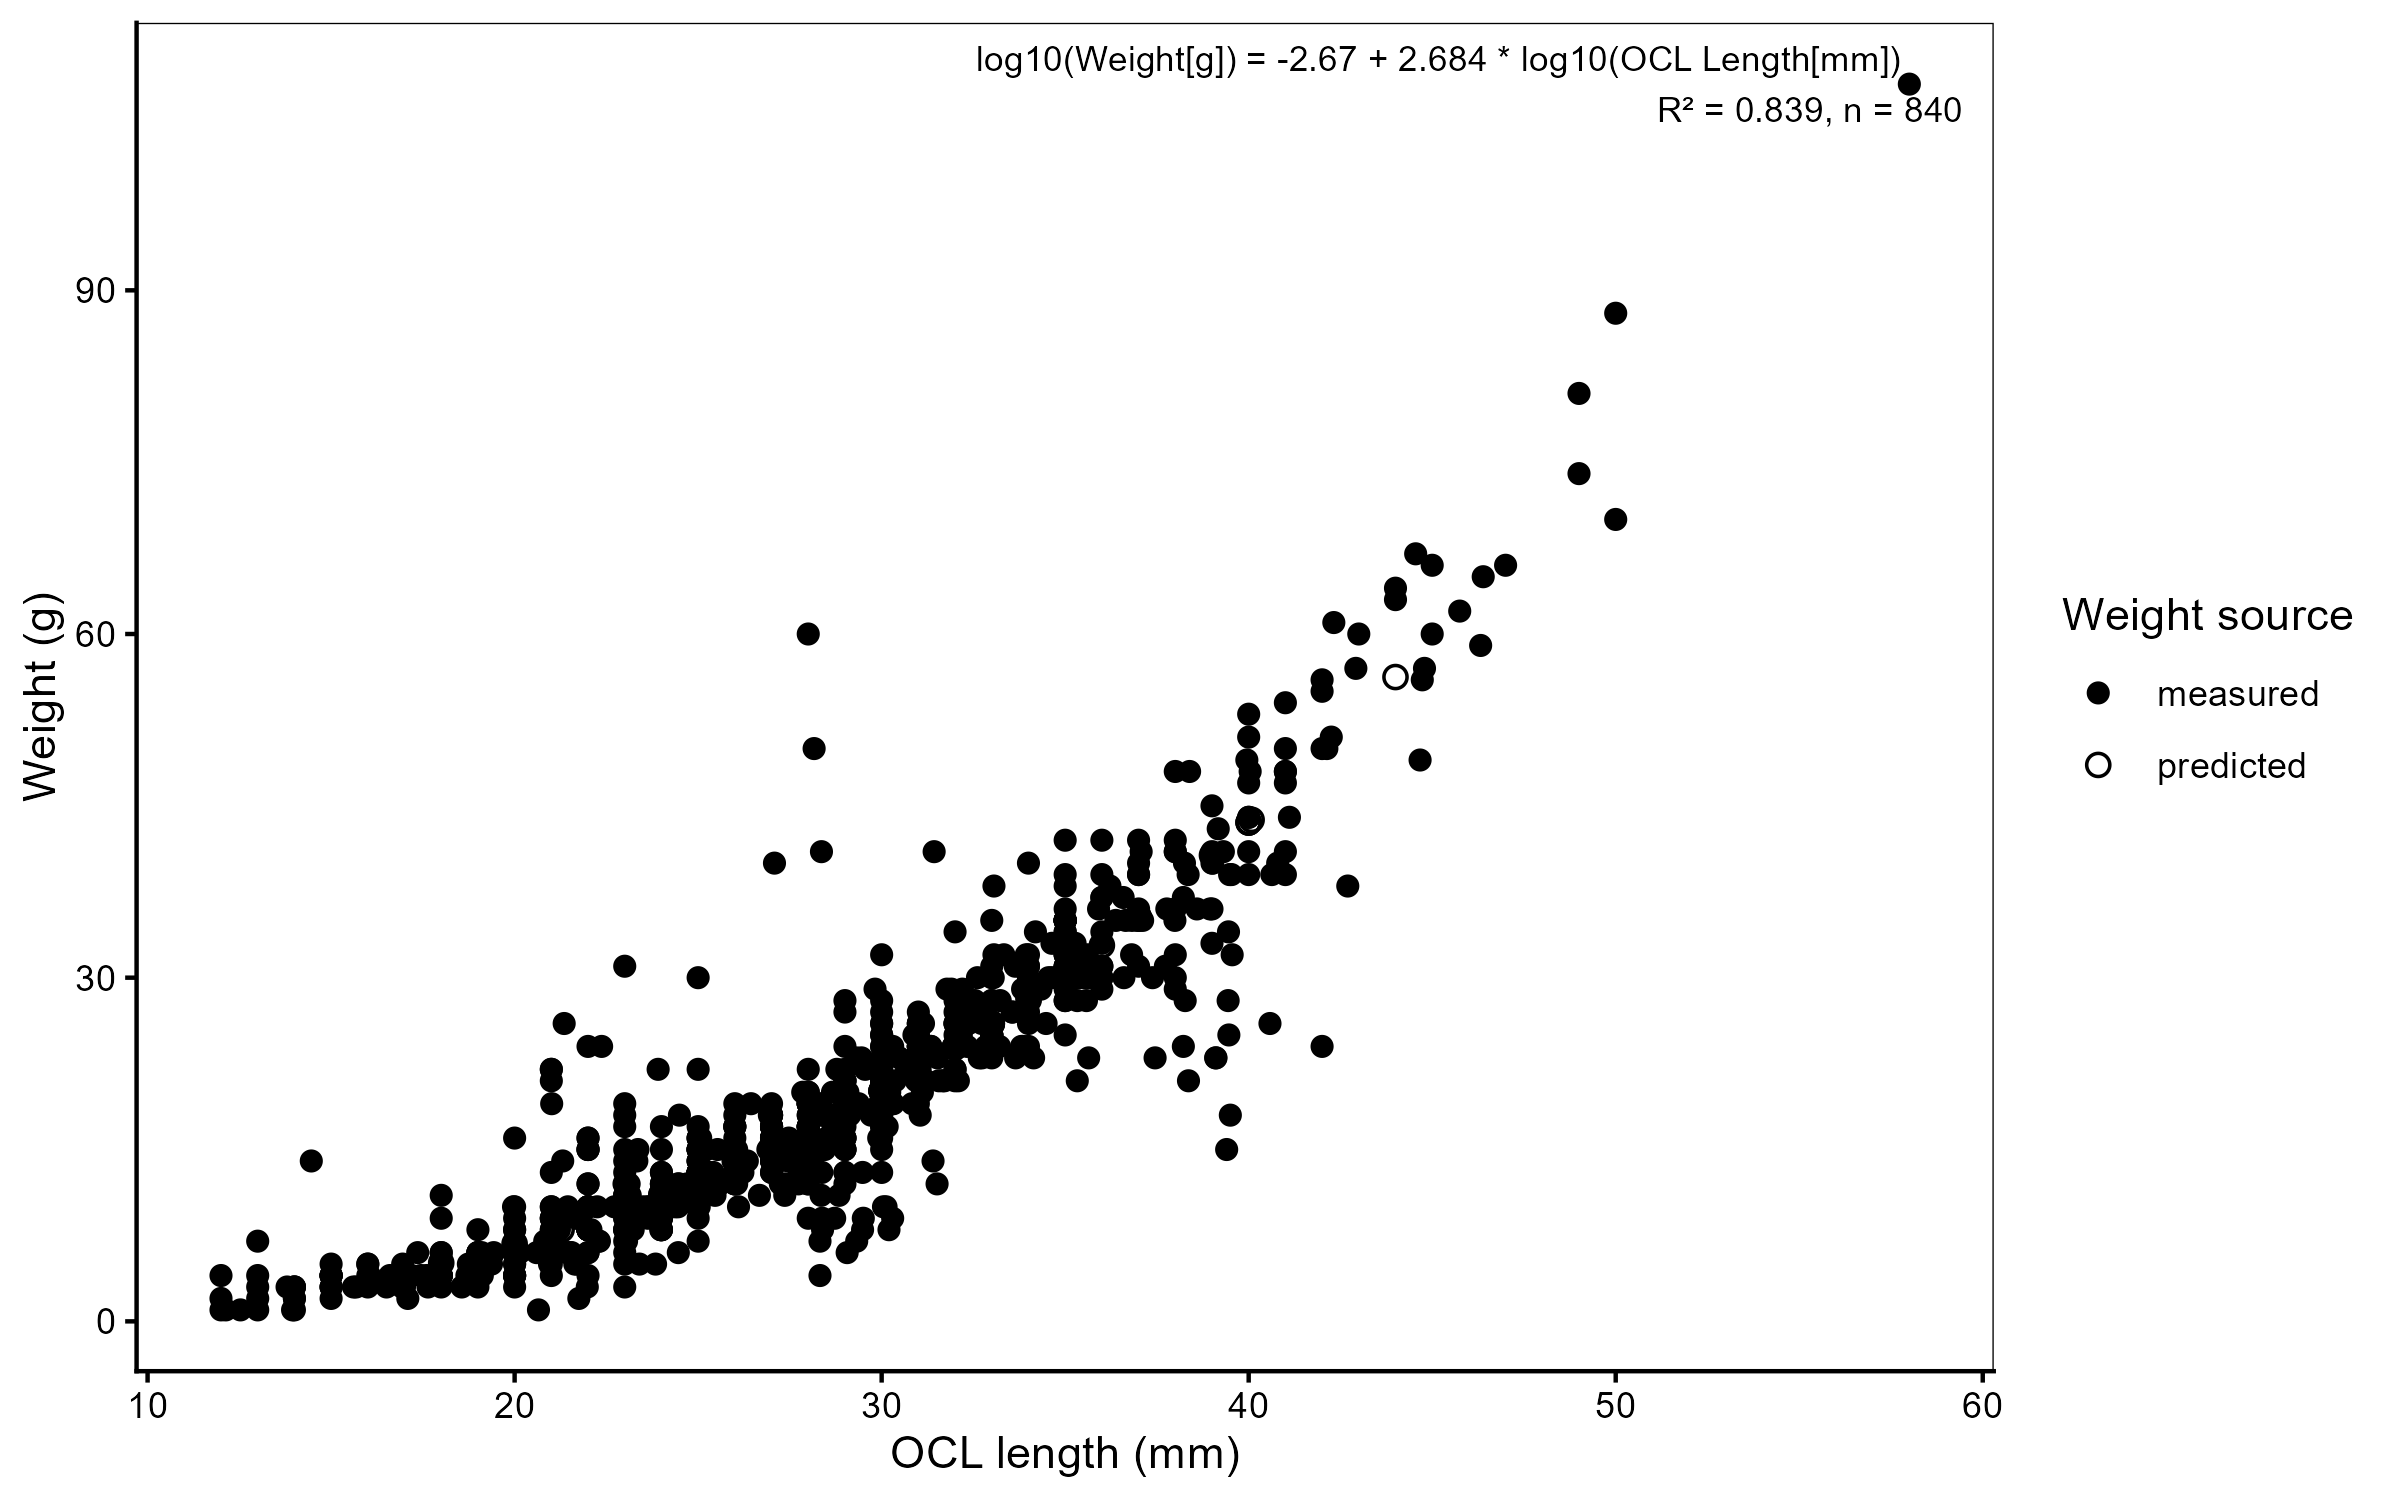
\includegraphics[width=0.8\linewidth,height=\textheight,keepaspectratio]{outputs/fig-length-weight-ch5.png}

}

\caption{\label{fig-length-weight-ch5}Length--weight relationship for
kōura, fitted on log₁₀--log₁₀ scale. Open points are weights predicted
from the length--weight regression (used to fill missing scale
measurements); filled points are directly measured weights.}

\end{figure}%

\begin{figure}

\centering{

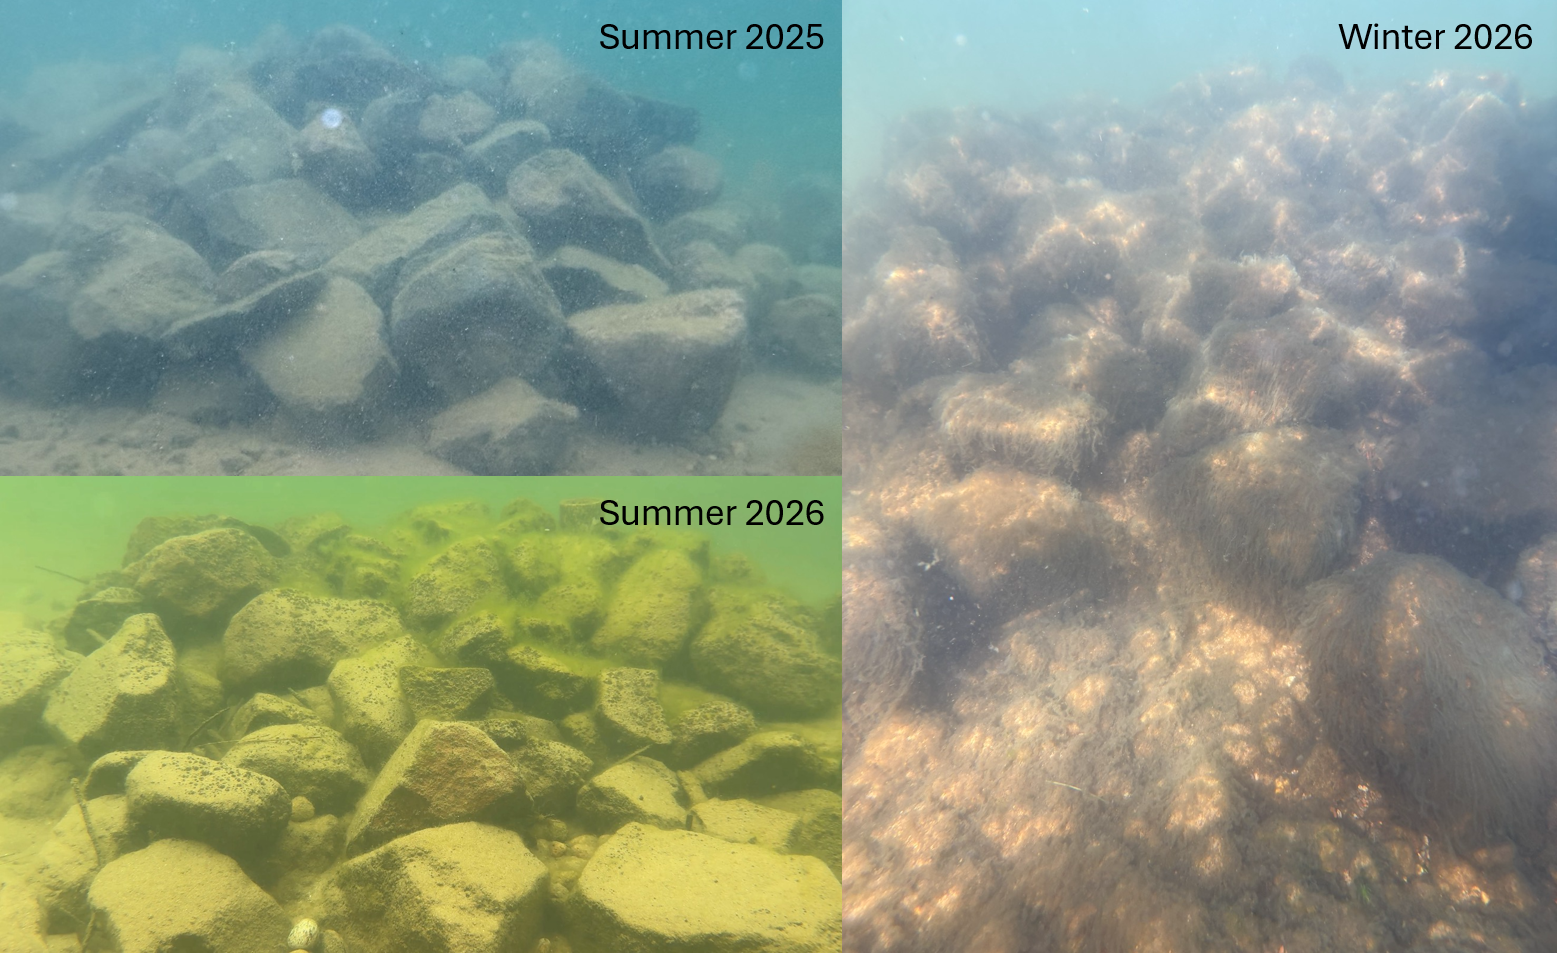
\includegraphics[width=0.8\linewidth,height=\textheight,keepaspectratio]{images/Stone_pile_development.png}

}

\caption{\label{fig-stone-piles}Progressive algal biofouling at stone
pile site 9 in Lake Rotoiti across three monitoring periods. Summer 2025
(top left, shortly after construction) shows clean stone surfaces.
Summer 2026 (bottom left) shows moderate biofilm accumulation. Winter
2026 (right) shows extensive cover of stone surfaces by filamentous
algae.}

\end{figure}%

\begin{landscape}\begingroup\fontsize{7}{9}\selectfont

\begin{longtable}[t]{lllllllrrrrrrr}

\caption{\label{tbl-models-summary-full-supp}Full fixed-effect estimates
(\(\beta\), SE, 95\% CI, p-value) for every term in every model.}

\tabularnewline

\toprule
model\_id & RQ & species & response\_type & comparison & time\_frame & term & estimate & std.error & statistic & p.value & p\_adj\_BH & conf.low & conf.high\\
\midrule
\endfirsthead
\multicolumn{14}{@{}l}{\textit{(continued)}}\\
\toprule
model\_id & RQ & species & response\_type & comparison & time\_frame & term & estimate & std.error & statistic & p.value & p\_adj\_BH & conf.low & conf.high\\
\midrule
\endhead

\endfoot
\bottomrule
\endlastfoot
\cellcolor{gray!8}{M1aac} & \cellcolor{gray!8}{RQ1} & \cellcolor{gray!8}{Catfish} & \cellcolor{gray!8}{abundance} & \cellcolor{gray!8}{treatment} & \cellcolor{gray!8}{before} & \cellcolor{gray!8}{(Intercept)} & \cellcolor{gray!8}{-2.303} & \cellcolor{gray!8}{0.908} & \cellcolor{gray!8}{-2.535} & \cellcolor{gray!8}{0.011} & \cellcolor{gray!8}{NA} & \cellcolor{gray!8}{-4.083} & \cellcolor{gray!8}{-0.522}\\
M1aac & RQ1 & Catfish & abundance & treatment & before & Site\_type\_detailStone\_pile & -0.693 & 1.535 & -0.452 & 0.652 & 0.783 & -3.701 & 2.315\\
\cellcolor{gray!8}{M1abc} & \cellcolor{gray!8}{RQ1} & \cellcolor{gray!8}{Catfish} & \cellcolor{gray!8}{biomass} & \cellcolor{gray!8}{treatment} & \cellcolor{gray!8}{before} & \cellcolor{gray!8}{(Intercept)} & \cellcolor{gray!8}{3.203} & \cellcolor{gray!8}{1.279} & \cellcolor{gray!8}{2.504} & \cellcolor{gray!8}{0.012} & \cellcolor{gray!8}{NA} & \cellcolor{gray!8}{0.696} & \cellcolor{gray!8}{5.709}\\
M1abc & RQ1 & Catfish & biomass & treatment & before & Site\_type\_detailStone\_pile & -5.100 & 3.107 & -1.641 & 0.101 & 0.403 & -11.190 & 0.990\\
\cellcolor{gray!8}{M1aak} & \cellcolor{gray!8}{RQ1} & \cellcolor{gray!8}{Kōura} & \cellcolor{gray!8}{abundance} & \cellcolor{gray!8}{treatment} & \cellcolor{gray!8}{before} & \cellcolor{gray!8}{(Intercept)} & \cellcolor{gray!8}{-1.897} & \cellcolor{gray!8}{0.785} & \cellcolor{gray!8}{-2.415} & \cellcolor{gray!8}{0.016} & \cellcolor{gray!8}{NA} & \cellcolor{gray!8}{-3.437} & \cellcolor{gray!8}{-0.358}\\
\addlinespace
M1aak & RQ1 & Kōura & abundance & treatment & before & Site\_type\_detailStone\_pile & 0.288 & 1.044 & 0.276 & 0.783 & 0.783 & -1.759 & 2.334\\
\cellcolor{gray!8}{M1abk} & \cellcolor{gray!8}{RQ1} & \cellcolor{gray!8}{Kōura} & \cellcolor{gray!8}{biomass} & \cellcolor{gray!8}{treatment} & \cellcolor{gray!8}{before} & \cellcolor{gray!8}{(Intercept)} & \cellcolor{gray!8}{1.030} & \cellcolor{gray!8}{0.830} & \cellcolor{gray!8}{1.241} & \cellcolor{gray!8}{0.215} & \cellcolor{gray!8}{NA} & \cellcolor{gray!8}{-0.597} & \cellcolor{gray!8}{2.656}\\
M1abk & RQ1 & Kōura & biomass & treatment & before & Site\_type\_detailStone\_pile & 1.044 & 0.977 & 1.068 & 0.286 & 0.571 & -0.872 & 2.959\\
\cellcolor{gray!8}{M1bac} & \cellcolor{gray!8}{RQ1} & \cellcolor{gray!8}{Catfish} & \cellcolor{gray!8}{abundance} & \cellcolor{gray!8}{reference} & \cellcolor{gray!8}{before} & \cellcolor{gray!8}{(Intercept)} & \cellcolor{gray!8}{-102.299} & \cellcolor{gray!8}{32.656} & \cellcolor{gray!8}{-3.133} & \cellcolor{gray!8}{0.002} & \cellcolor{gray!8}{NA} & \cellcolor{gray!8}{-166.303} & \cellcolor{gray!8}{-38.295}\\
M1bac & RQ1 & Catfish & abundance & reference & before & Site\_type\_detailReference\_2 & -1.655 & 0.536 & -3.087 & 0.002 & 0.004 & -2.706 & -0.604\\
\addlinespace
\cellcolor{gray!8}{M1bac} & \cellcolor{gray!8}{RQ1} & \cellcolor{gray!8}{Catfish} & \cellcolor{gray!8}{abundance} & \cellcolor{gray!8}{reference} & \cellcolor{gray!8}{before} & \cellcolor{gray!8}{Temperature} & \cellcolor{gray!8}{4.079} & \cellcolor{gray!8}{1.293} & \cellcolor{gray!8}{3.154} & \cellcolor{gray!8}{0.002} & \cellcolor{gray!8}{NA} & \cellcolor{gray!8}{1.544} & \cellcolor{gray!8}{6.613}\\
M1bbc & RQ1 & Catfish & biomass & reference & before & (Intercept) & -153.136 & 37.363 & -4.099 & 0.000 & NA & -226.366 & -79.906\\
\cellcolor{gray!8}{M1bbc} & \cellcolor{gray!8}{RQ1} & \cellcolor{gray!8}{Catfish} & \cellcolor{gray!8}{biomass} & \cellcolor{gray!8}{reference} & \cellcolor{gray!8}{before} & \cellcolor{gray!8}{Site\_type\_detailReference\_2} & \cellcolor{gray!8}{-2.569} & \cellcolor{gray!8}{0.743} & \cellcolor{gray!8}{-3.457} & \cellcolor{gray!8}{0.001} & \cellcolor{gray!8}{0.002} & \cellcolor{gray!8}{-4.026} & \cellcolor{gray!8}{-1.112}\\
M1bbc & RQ1 & Catfish & biomass & reference & before & Temperature & 6.315 & 1.482 & 4.261 & 0.000 & NA & 3.410 & 9.220\\
\cellcolor{gray!8}{M1bak} & \cellcolor{gray!8}{RQ1} & \cellcolor{gray!8}{Kōura} & \cellcolor{gray!8}{abundance} & \cellcolor{gray!8}{reference} & \cellcolor{gray!8}{before} & \cellcolor{gray!8}{(Intercept)} & \cellcolor{gray!8}{0.742} & \cellcolor{gray!8}{0.553} & \cellcolor{gray!8}{1.343} & \cellcolor{gray!8}{0.179} & \cellcolor{gray!8}{NA} & \cellcolor{gray!8}{-0.341} & \cellcolor{gray!8}{1.825}\\
\addlinespace
M1bak & RQ1 & Kōura & abundance & reference & before & Site\_type\_detailReference\_2 & 0.031 & 0.778 & 0.040 & 0.968 & 0.968 & -1.494 & 1.557\\
\cellcolor{gray!8}{M1bbk} & \cellcolor{gray!8}{RQ1} & \cellcolor{gray!8}{Kōura} & \cellcolor{gray!8}{biomass} & \cellcolor{gray!8}{reference} & \cellcolor{gray!8}{before} & \cellcolor{gray!8}{(Intercept)} & \cellcolor{gray!8}{3.623} & \cellcolor{gray!8}{0.478} & \cellcolor{gray!8}{7.580} & \cellcolor{gray!8}{0.000} & \cellcolor{gray!8}{NA} & \cellcolor{gray!8}{2.686} & \cellcolor{gray!8}{4.560}\\
M1bbk & RQ1 & Kōura & biomass & reference & before & Site\_type\_detailReference\_2 & -0.041 & 0.681 & -0.061 & 0.952 & 0.968 & -1.375 & 1.293\\
\cellcolor{gray!8}{M2aac} & \cellcolor{gray!8}{RQ2a} & \cellcolor{gray!8}{Catfish} & \cellcolor{gray!8}{abundance} & \cellcolor{gray!8}{vs\_control} & \cellcolor{gray!8}{full} & \cellcolor{gray!8}{(Intercept)} & \cellcolor{gray!8}{-3.976} & \cellcolor{gray!8}{1.631} & \cellcolor{gray!8}{-2.438} & \cellcolor{gray!8}{0.015} & \cellcolor{gray!8}{NA} & \cellcolor{gray!8}{-7.173} & \cellcolor{gray!8}{-0.780}\\
M2aac & RQ2a & Catfish & abundance & vs\_control & full & PeriodAfter & 0.673 & 1.521 & 0.442 & 0.658 & NA & -2.308 & 3.654\\
\addlinespace
\cellcolor{gray!8}{M2aac} & \cellcolor{gray!8}{RQ2a} & \cellcolor{gray!8}{Catfish} & \cellcolor{gray!8}{abundance} & \cellcolor{gray!8}{vs\_control} & \cellcolor{gray!8}{full} & \cellcolor{gray!8}{siteStone\_pile} & \cellcolor{gray!8}{-0.639} & \cellcolor{gray!8}{1.762} & \cellcolor{gray!8}{-0.362} & \cellcolor{gray!8}{0.717} & \cellcolor{gray!8}{NA} & \cellcolor{gray!8}{-4.093} & \cellcolor{gray!8}{2.816}\\
M2aac & RQ2a & Catfish & abundance & vs\_control & full & monitoring\_int & -0.294 & 0.344 & -0.853 & 0.394 & NA & -0.968 & 0.381\\
\cellcolor{gray!8}{M2aac} & \cellcolor{gray!8}{RQ2a} & \cellcolor{gray!8}{Catfish} & \cellcolor{gray!8}{abundance} & \cellcolor{gray!8}{vs\_control} & \cellcolor{gray!8}{full} & \cellcolor{gray!8}{fetch\_z} & \cellcolor{gray!8}{-1.194} & \cellcolor{gray!8}{1.077} & \cellcolor{gray!8}{-1.109} & \cellcolor{gray!8}{0.267} & \cellcolor{gray!8}{NA} & \cellcolor{gray!8}{-3.305} & \cellcolor{gray!8}{0.916}\\
M2aac & RQ2a & Catfish & abundance & vs\_control & full & PeriodAfter:siteStone\_pile & 2.002 & 1.973 & 1.015 & 0.310 & 0.858 & -1.864 & 5.869\\
\cellcolor{gray!8}{M2abc} & \cellcolor{gray!8}{RQ2a} & \cellcolor{gray!8}{Catfish} & \cellcolor{gray!8}{biomass} & \cellcolor{gray!8}{vs\_control} & \cellcolor{gray!8}{full} & \cellcolor{gray!8}{(Intercept)} & \cellcolor{gray!8}{0.202} & \cellcolor{gray!8}{4.319} & \cellcolor{gray!8}{0.047} & \cellcolor{gray!8}{0.963} & \cellcolor{gray!8}{NA} & \cellcolor{gray!8}{-8.262} & \cellcolor{gray!8}{8.667}\\
\addlinespace
M2abc & RQ2a & Catfish & biomass & vs\_control & full & PeriodAfter & -0.340 & 2.404 & -0.141 & 0.888 & NA & -5.052 & 4.372\\
\cellcolor{gray!8}{M2abc} & \cellcolor{gray!8}{RQ2a} & \cellcolor{gray!8}{Catfish} & \cellcolor{gray!8}{biomass} & \cellcolor{gray!8}{vs\_control} & \cellcolor{gray!8}{full} & \cellcolor{gray!8}{siteStone\_pile} & \cellcolor{gray!8}{-5.574} & \cellcolor{gray!8}{7.158} & \cellcolor{gray!8}{-0.779} & \cellcolor{gray!8}{0.436} & \cellcolor{gray!8}{NA} & \cellcolor{gray!8}{-19.604} & \cellcolor{gray!8}{8.456}\\
M2abc & RQ2a & Catfish & biomass & vs\_control & full & monitoring\_int & -0.381 & 0.523 & -0.728 & 0.466 & NA & -1.406 & 0.644\\
\cellcolor{gray!8}{M2abc} & \cellcolor{gray!8}{RQ2a} & \cellcolor{gray!8}{Catfish} & \cellcolor{gray!8}{biomass} & \cellcolor{gray!8}{vs\_control} & \cellcolor{gray!8}{full} & \cellcolor{gray!8}{fetch\_z} & \cellcolor{gray!8}{-1.675} & \cellcolor{gray!8}{2.438} & \cellcolor{gray!8}{-0.687} & \cellcolor{gray!8}{0.492} & \cellcolor{gray!8}{NA} & \cellcolor{gray!8}{-6.454} & \cellcolor{gray!8}{3.103}\\
M2abc & RQ2a & Catfish & biomass & vs\_control & full & PeriodAfter:siteStone\_pile & 5.436 & 5.592 & 0.972 & 0.331 & 0.858 & -5.524 & 16.396\\
\addlinespace
\cellcolor{gray!8}{M2aoc} & \cellcolor{gray!8}{RQ2a} & \cellcolor{gray!8}{Catfish} & \cellcolor{gray!8}{occupancy} & \cellcolor{gray!8}{vs\_control} & \cellcolor{gray!8}{full} & \cellcolor{gray!8}{(Intercept)} & \cellcolor{gray!8}{-2.185} & \cellcolor{gray!8}{1.887} & \cellcolor{gray!8}{-1.158} & \cellcolor{gray!8}{0.247} & \cellcolor{gray!8}{NA} & \cellcolor{gray!8}{-5.883} & \cellcolor{gray!8}{1.513}\\
M2aoc & RQ2a & Catfish & occupancy & vs\_control & full & PeriodAfter & -0.161 & 1.765 & -0.091 & 0.927 & NA & -3.621 & 3.299\\
\cellcolor{gray!8}{M2aoc} & \cellcolor{gray!8}{RQ2a} & \cellcolor{gray!8}{Catfish} & \cellcolor{gray!8}{occupancy} & \cellcolor{gray!8}{vs\_control} & \cellcolor{gray!8}{full} & \cellcolor{gray!8}{siteStone\_pile} & \cellcolor{gray!8}{0.024} & \cellcolor{gray!8}{1.982} & \cellcolor{gray!8}{0.012} & \cellcolor{gray!8}{0.990} & \cellcolor{gray!8}{NA} & \cellcolor{gray!8}{-3.860} & \cellcolor{gray!8}{3.909}\\
M2aoc & RQ2a & Catfish & occupancy & vs\_control & full & monitoring\_int & -0.165 & 0.259 & -0.635 & 0.525 & NA & -0.673 & 0.343\\
\cellcolor{gray!8}{M2aoc} & \cellcolor{gray!8}{RQ2a} & \cellcolor{gray!8}{Catfish} & \cellcolor{gray!8}{occupancy} & \cellcolor{gray!8}{vs\_control} & \cellcolor{gray!8}{full} & \cellcolor{gray!8}{fetch\_z} & \cellcolor{gray!8}{-0.960} & \cellcolor{gray!8}{1.197} & \cellcolor{gray!8}{-0.802} & \cellcolor{gray!8}{0.423} & \cellcolor{gray!8}{NA} & \cellcolor{gray!8}{-3.306} & \cellcolor{gray!8}{1.387}\\
\addlinespace
M2aoc & RQ2a & Catfish & occupancy & vs\_control & full & PeriodAfter:siteStone\_pile & 0.387 & 2.168 & 0.179 & 0.858 & 0.858 & -3.863 & 4.637\\
\cellcolor{gray!8}{M2aak} & \cellcolor{gray!8}{RQ2a} & \cellcolor{gray!8}{Kōura} & \cellcolor{gray!8}{abundance} & \cellcolor{gray!8}{vs\_control} & \cellcolor{gray!8}{full} & \cellcolor{gray!8}{(Intercept)} & \cellcolor{gray!8}{-2.753} & \cellcolor{gray!8}{1.183} & \cellcolor{gray!8}{-2.327} & \cellcolor{gray!8}{0.020} & \cellcolor{gray!8}{NA} & \cellcolor{gray!8}{-5.072} & \cellcolor{gray!8}{-0.434}\\
M2aak & RQ2a & Kōura & abundance & vs\_control & full & PeriodAfter & 2.374 & 0.976 & 2.432 & 0.015 & NA & 0.461 & 4.286\\
\cellcolor{gray!8}{M2aak} & \cellcolor{gray!8}{RQ2a} & \cellcolor{gray!8}{Kōura} & \cellcolor{gray!8}{abundance} & \cellcolor{gray!8}{vs\_control} & \cellcolor{gray!8}{full} & \cellcolor{gray!8}{siteStone\_pile} & \cellcolor{gray!8}{0.751} & \cellcolor{gray!8}{1.335} & \cellcolor{gray!8}{0.563} & \cellcolor{gray!8}{0.574} & \cellcolor{gray!8}{NA} & \cellcolor{gray!8}{-1.865} & \cellcolor{gray!8}{3.368}\\
M2aak & RQ2a & Kōura & abundance & vs\_control & full & monitoring\_int & -0.253 & 0.082 & -3.094 & 0.002 & NA & -0.413 & -0.093\\
\addlinespace
\cellcolor{gray!8}{M2aak} & \cellcolor{gray!8}{RQ2a} & \cellcolor{gray!8}{Kōura} & \cellcolor{gray!8}{abundance} & \cellcolor{gray!8}{vs\_control} & \cellcolor{gray!8}{full} & \cellcolor{gray!8}{PeriodAfter:siteStone\_pile} & \cellcolor{gray!8}{0.311} & \cellcolor{gray!8}{1.232} & \cellcolor{gray!8}{0.253} & \cellcolor{gray!8}{0.800} & \cellcolor{gray!8}{0.858} & \cellcolor{gray!8}{-2.104} & \cellcolor{gray!8}{2.727}\\
M2abk & RQ2a & Kōura & biomass & vs\_control & full & (Intercept) & 0.315 & 1.335 & 0.236 & 0.813 & NA & -2.301 & 2.931\\
\cellcolor{gray!8}{M2abk} & \cellcolor{gray!8}{RQ2a} & \cellcolor{gray!8}{Kōura} & \cellcolor{gray!8}{biomass} & \cellcolor{gray!8}{vs\_control} & \cellcolor{gray!8}{full} & \cellcolor{gray!8}{PeriodAfter} & \cellcolor{gray!8}{2.248} & \cellcolor{gray!8}{1.246} & \cellcolor{gray!8}{1.805} & \cellcolor{gray!8}{0.071} & \cellcolor{gray!8}{NA} & \cellcolor{gray!8}{-0.193} & \cellcolor{gray!8}{4.689}\\
M2abk & RQ2a & Kōura & biomass & vs\_control & full & siteStone\_pile & 1.410 & 1.552 & 0.909 & 0.363 & NA & -1.631 & 4.451\\
\cellcolor{gray!8}{M2abk} & \cellcolor{gray!8}{RQ2a} & \cellcolor{gray!8}{Kōura} & \cellcolor{gray!8}{biomass} & \cellcolor{gray!8}{vs\_control} & \cellcolor{gray!8}{full} & \cellcolor{gray!8}{monitoring\_int} & \cellcolor{gray!8}{-0.196} & \cellcolor{gray!8}{0.110} & \cellcolor{gray!8}{-1.791} & \cellcolor{gray!8}{0.073} & \cellcolor{gray!8}{NA} & \cellcolor{gray!8}{-0.412} & \cellcolor{gray!8}{0.019}\\
\addlinespace
M2abk & RQ2a & Kōura & biomass & vs\_control & full & PeriodAfter:siteStone\_pile & -0.336 & 1.471 & -0.228 & 0.819 & 0.858 & -3.220 & 2.548\\
\cellcolor{gray!8}{M2aok} & \cellcolor{gray!8}{RQ2a} & \cellcolor{gray!8}{Kōura} & \cellcolor{gray!8}{occupancy} & \cellcolor{gray!8}{vs\_control} & \cellcolor{gray!8}{full} & \cellcolor{gray!8}{(Intercept)} & \cellcolor{gray!8}{-0.690} & \cellcolor{gray!8}{1.643} & \cellcolor{gray!8}{-0.420} & \cellcolor{gray!8}{0.674} & \cellcolor{gray!8}{NA} & \cellcolor{gray!8}{-3.911} & \cellcolor{gray!8}{2.530}\\
M2aok & RQ2a & Kōura & occupancy & vs\_control & full & PeriodAfter & 1.913 & 1.556 & 1.230 & 0.219 & NA & -1.136 & 4.963\\
\cellcolor{gray!8}{M2aok} & \cellcolor{gray!8}{RQ2a} & \cellcolor{gray!8}{Kōura} & \cellcolor{gray!8}{occupancy} & \cellcolor{gray!8}{vs\_control} & \cellcolor{gray!8}{full} & \cellcolor{gray!8}{siteStone\_pile} & \cellcolor{gray!8}{0.013} & \cellcolor{gray!8}{2.121} & \cellcolor{gray!8}{0.006} & \cellcolor{gray!8}{0.995} & \cellcolor{gray!8}{NA} & \cellcolor{gray!8}{-4.144} & \cellcolor{gray!8}{4.171}\\
M2aok & RQ2a & Kōura & occupancy & vs\_control & full & monitoring\_int & -0.286 & 0.215 & -1.333 & 0.183 & NA & -0.708 & 0.135\\
\addlinespace
\cellcolor{gray!8}{M2aok} & \cellcolor{gray!8}{RQ2a} & \cellcolor{gray!8}{Kōura} & \cellcolor{gray!8}{occupancy} & \cellcolor{gray!8}{vs\_control} & \cellcolor{gray!8}{full} & \cellcolor{gray!8}{PeriodAfter:siteStone\_pile} & \cellcolor{gray!8}{1.013} & \cellcolor{gray!8}{1.762} & \cellcolor{gray!8}{0.575} & \cellcolor{gray!8}{0.565} & \cellcolor{gray!8}{0.858} & \cellcolor{gray!8}{-2.440} & \cellcolor{gray!8}{4.466}\\
M2bac & RQ2b & Catfish & abundance & vs\_control & after & (Intercept) & -2.150 & 1.519 & -1.416 & 0.157 & NA & -5.127 & 0.826\\
\cellcolor{gray!8}{M2bac} & \cellcolor{gray!8}{RQ2b} & \cellcolor{gray!8}{Catfish} & \cellcolor{gray!8}{abundance} & \cellcolor{gray!8}{vs\_control} & \cellcolor{gray!8}{after} & \cellcolor{gray!8}{siteStone\_pile} & \cellcolor{gray!8}{-1.392} & \cellcolor{gray!8}{1.832} & \cellcolor{gray!8}{-0.760} & \cellcolor{gray!8}{0.447} & \cellcolor{gray!8}{NA} & \cellcolor{gray!8}{-4.983} & \cellcolor{gray!8}{2.199}\\
M2bac & RQ2b & Catfish & abundance & vs\_control & after & monitoring\_int & -0.634 & 0.406 & -1.562 & 0.118 & NA & -1.430 & 0.162\\
\cellcolor{gray!8}{M2bac} & \cellcolor{gray!8}{RQ2b} & \cellcolor{gray!8}{Catfish} & \cellcolor{gray!8}{abundance} & \cellcolor{gray!8}{vs\_control} & \cellcolor{gray!8}{after} & \cellcolor{gray!8}{fetch\_z} & \cellcolor{gray!8}{-1.097} & \cellcolor{gray!8}{0.976} & \cellcolor{gray!8}{-1.124} & \cellcolor{gray!8}{0.261} & \cellcolor{gray!8}{NA} & \cellcolor{gray!8}{-3.010} & \cellcolor{gray!8}{0.816}\\
\addlinespace
M2bac & RQ2b & Catfish & abundance & vs\_control & after & siteStone\_pile:monitoring\_int & 0.831 & 0.557 & 1.492 & 0.136 & 0.215 & -0.261 & 1.922\\
\cellcolor{gray!8}{M2bbc} & \cellcolor{gray!8}{RQ2b} & \cellcolor{gray!8}{Catfish} & \cellcolor{gray!8}{biomass} & \cellcolor{gray!8}{vs\_control} & \cellcolor{gray!8}{after} & \cellcolor{gray!8}{(Intercept)} & \cellcolor{gray!8}{2.964} & \cellcolor{gray!8}{2.725} & \cellcolor{gray!8}{1.088} & \cellcolor{gray!8}{0.277} & \cellcolor{gray!8}{NA} & \cellcolor{gray!8}{-2.377} & \cellcolor{gray!8}{8.304}\\
M2bbc & RQ2b & Catfish & biomass & vs\_control & after & siteStone\_pile & -4.522 & 4.240 & -1.066 & 0.286 & NA & -12.833 & 3.789\\
\cellcolor{gray!8}{M2bbc} & \cellcolor{gray!8}{RQ2b} & \cellcolor{gray!8}{Catfish} & \cellcolor{gray!8}{biomass} & \cellcolor{gray!8}{vs\_control} & \cellcolor{gray!8}{after} & \cellcolor{gray!8}{monitoring\_int} & \cellcolor{gray!8}{-0.974} & \cellcolor{gray!8}{0.688} & \cellcolor{gray!8}{-1.416} & \cellcolor{gray!8}{0.157} & \cellcolor{gray!8}{NA} & \cellcolor{gray!8}{-2.323} & \cellcolor{gray!8}{0.374}\\
M2bbc & RQ2b & Catfish & biomass & vs\_control & after & fetch\_z & -0.886 & 1.390 & -0.638 & 0.524 & NA & -3.610 & 1.837\\
\addlinespace
\cellcolor{gray!8}{M2bbc} & \cellcolor{gray!8}{RQ2b} & \cellcolor{gray!8}{Catfish} & \cellcolor{gray!8}{biomass} & \cellcolor{gray!8}{vs\_control} & \cellcolor{gray!8}{after} & \cellcolor{gray!8}{siteStone\_pile:monitoring\_int} & \cellcolor{gray!8}{1.357} & \cellcolor{gray!8}{0.974} & \cellcolor{gray!8}{1.393} & \cellcolor{gray!8}{0.164} & \cellcolor{gray!8}{0.215} & \cellcolor{gray!8}{-0.552} & \cellcolor{gray!8}{3.266}\\
M2boc & RQ2b & Catfish & occupancy & vs\_control & after & (Intercept) & -0.952 & 1.737 & -0.548 & 0.584 & NA & -4.357 & 2.453\\
\cellcolor{gray!8}{M2boc} & \cellcolor{gray!8}{RQ2b} & \cellcolor{gray!8}{Catfish} & \cellcolor{gray!8}{occupancy} & \cellcolor{gray!8}{vs\_control} & \cellcolor{gray!8}{after} & \cellcolor{gray!8}{siteStone\_pile} & \cellcolor{gray!8}{-2.013} & \cellcolor{gray!8}{1.936} & \cellcolor{gray!8}{-1.040} & \cellcolor{gray!8}{0.298} & \cellcolor{gray!8}{NA} & \cellcolor{gray!8}{-5.808} & \cellcolor{gray!8}{1.781}\\
M2boc & RQ2b & Catfish & occupancy & vs\_control & after & monitoring\_int & -0.565 & 0.420 & -1.345 & 0.179 & NA & -1.388 & 0.258\\
\cellcolor{gray!8}{M2boc} & \cellcolor{gray!8}{RQ2b} & \cellcolor{gray!8}{Catfish} & \cellcolor{gray!8}{occupancy} & \cellcolor{gray!8}{vs\_control} & \cellcolor{gray!8}{after} & \cellcolor{gray!8}{fetch\_z} & \cellcolor{gray!8}{-0.858} & \cellcolor{gray!8}{1.121} & \cellcolor{gray!8}{-0.766} & \cellcolor{gray!8}{0.444} & \cellcolor{gray!8}{NA} & \cellcolor{gray!8}{-3.055} & \cellcolor{gray!8}{1.339}\\
\addlinespace
M2boc & RQ2b & Catfish & occupancy & vs\_control & after & siteStone\_pile:monitoring\_int & 0.735 & 0.546 & 1.344 & 0.179 & 0.215 & -0.336 & 1.806\\
\cellcolor{gray!8}{M2bak} & \cellcolor{gray!8}{RQ2b} & \cellcolor{gray!8}{Kōura} & \cellcolor{gray!8}{abundance} & \cellcolor{gray!8}{vs\_control} & \cellcolor{gray!8}{after} & \cellcolor{gray!8}{(Intercept)} & \cellcolor{gray!8}{0.084} & \cellcolor{gray!8}{0.846} & \cellcolor{gray!8}{0.099} & \cellcolor{gray!8}{0.921} & \cellcolor{gray!8}{NA} & \cellcolor{gray!8}{-1.573} & \cellcolor{gray!8}{1.741}\\
M2bak & RQ2b & Kōura & abundance & vs\_control & after & siteStone\_pile & 0.323 & 0.808 & 0.400 & 0.689 & NA & -1.261 & 1.907\\
\cellcolor{gray!8}{M2bak} & \cellcolor{gray!8}{RQ2b} & \cellcolor{gray!8}{Kōura} & \cellcolor{gray!8}{abundance} & \cellcolor{gray!8}{vs\_control} & \cellcolor{gray!8}{after} & \cellcolor{gray!8}{monitoring\_int} & \cellcolor{gray!8}{-0.409} & \cellcolor{gray!8}{0.143} & \cellcolor{gray!8}{-2.861} & \cellcolor{gray!8}{0.004} & \cellcolor{gray!8}{NA} & \cellcolor{gray!8}{-0.690} & \cellcolor{gray!8}{-0.129}\\
M2bak & RQ2b & Kōura & abundance & vs\_control & after & siteStone\_pile:monitoring\_int & 0.243 & 0.179 & 1.359 & 0.174 & 0.215 & -0.107 & 0.593\\
\addlinespace
\cellcolor{gray!8}{M2bbk} & \cellcolor{gray!8}{RQ2b} & \cellcolor{gray!8}{Kōura} & \cellcolor{gray!8}{biomass} & \cellcolor{gray!8}{vs\_control} & \cellcolor{gray!8}{after} & \cellcolor{gray!8}{(Intercept)} & \cellcolor{gray!8}{3.270} & \cellcolor{gray!8}{0.856} & \cellcolor{gray!8}{3.821} & \cellcolor{gray!8}{0.000} & \cellcolor{gray!8}{NA} & \cellcolor{gray!8}{1.593} & \cellcolor{gray!8}{4.948}\\
M2bbk & RQ2b & Kōura & biomass & vs\_control & after & siteStone\_pile & -0.077 & 0.986 & -0.078 & 0.938 & NA & -2.010 & 1.856\\
\cellcolor{gray!8}{M2bbk} & \cellcolor{gray!8}{RQ2b} & \cellcolor{gray!8}{Kōura} & \cellcolor{gray!8}{biomass} & \cellcolor{gray!8}{vs\_control} & \cellcolor{gray!8}{after} & \cellcolor{gray!8}{monitoring\_int} & \cellcolor{gray!8}{-0.427} & \cellcolor{gray!8}{0.191} & \cellcolor{gray!8}{-2.240} & \cellcolor{gray!8}{0.025} & \cellcolor{gray!8}{NA} & \cellcolor{gray!8}{-0.800} & \cellcolor{gray!8}{-0.053}\\
M2bbk & RQ2b & Kōura & biomass & vs\_control & after & siteStone\_pile:monitoring\_int & 0.366 & 0.239 & 1.531 & 0.126 & 0.215 & -0.103 & 0.834\\
\cellcolor{gray!8}{M2bok} & \cellcolor{gray!8}{RQ2b} & \cellcolor{gray!8}{Kōura} & \cellcolor{gray!8}{occupancy} & \cellcolor{gray!8}{vs\_control} & \cellcolor{gray!8}{after} & \cellcolor{gray!8}{(Intercept)} & \cellcolor{gray!8}{1.585} & \cellcolor{gray!8}{1.885} & \cellcolor{gray!8}{0.841} & \cellcolor{gray!8}{0.400} & \cellcolor{gray!8}{NA} & \cellcolor{gray!8}{-2.109} & \cellcolor{gray!8}{5.280}\\
\addlinespace
M2bok & RQ2b & Kōura & occupancy & vs\_control & after & siteStone\_pile & 0.563 & 2.660 & 0.212 & 0.832 & NA & -4.651 & 5.776\\
\cellcolor{gray!8}{M2bok} & \cellcolor{gray!8}{RQ2b} & \cellcolor{gray!8}{Kōura} & \cellcolor{gray!8}{occupancy} & \cellcolor{gray!8}{vs\_control} & \cellcolor{gray!8}{after} & \cellcolor{gray!8}{monitoring\_int} & \cellcolor{gray!8}{-0.403} & \cellcolor{gray!8}{0.311} & \cellcolor{gray!8}{-1.296} & \cellcolor{gray!8}{0.195} & \cellcolor{gray!8}{NA} & \cellcolor{gray!8}{-1.014} & \cellcolor{gray!8}{0.207}\\
M2bok & RQ2b & Kōura & occupancy & vs\_control & after & siteStone\_pile:monitoring\_int & 0.229 & 0.441 & 0.519 & 0.604 & 0.604 & -0.636 & 1.094\\
\cellcolor{gray!8}{M3aac} & \cellcolor{gray!8}{RQ3a} & \cellcolor{gray!8}{Catfish} & \cellcolor{gray!8}{abundance} & \cellcolor{gray!8}{vs\_reference} & \cellcolor{gray!8}{after} & \cellcolor{gray!8}{(Intercept)} & \cellcolor{gray!8}{-7.151} & \cellcolor{gray!8}{1.282} & \cellcolor{gray!8}{-5.577} & \cellcolor{gray!8}{0.000} & \cellcolor{gray!8}{NA} & \cellcolor{gray!8}{-9.664} & \cellcolor{gray!8}{-4.638}\\
M3aac & RQ3a & Catfish & abundance & vs\_reference & after & siteStone\_pile & -2.471 & 1.940 & -1.274 & 0.203 & NA & -6.273 & 1.331\\
\addlinespace
\cellcolor{gray!8}{M3aac} & \cellcolor{gray!8}{RQ3a} & \cellcolor{gray!8}{Catfish} & \cellcolor{gray!8}{abundance} & \cellcolor{gray!8}{vs\_reference} & \cellcolor{gray!8}{after} & \cellcolor{gray!8}{monitoring\_int} & \cellcolor{gray!8}{-0.215} & \cellcolor{gray!8}{0.147} & \cellcolor{gray!8}{-1.462} & \cellcolor{gray!8}{0.144} & \cellcolor{gray!8}{NA} & \cellcolor{gray!8}{-0.504} & \cellcolor{gray!8}{0.073}\\
M3aac & RQ3a & Catfish & abundance & vs\_reference & after & Temperature & 0.315 & 0.058 & 5.414 & 0.000 & NA & 0.201 & 0.429\\
\cellcolor{gray!8}{M3aac} & \cellcolor{gray!8}{RQ3a} & \cellcolor{gray!8}{Catfish} & \cellcolor{gray!8}{abundance} & \cellcolor{gray!8}{vs\_reference} & \cellcolor{gray!8}{after} & \cellcolor{gray!8}{siteStone\_pile:monitoring\_int} & \cellcolor{gray!8}{0.510} & \cellcolor{gray!8}{0.398} & \cellcolor{gray!8}{1.283} & \cellcolor{gray!8}{0.199} & \cellcolor{gray!8}{0.559} & \cellcolor{gray!8}{-0.269} & \cellcolor{gray!8}{1.290}\\
M3abc & RQ3a & Catfish & biomass & vs\_reference & after & (Intercept) & 3.011 & 1.189 & 2.532 & 0.011 & NA & 0.681 & 5.342\\
\cellcolor{gray!8}{M3abc} & \cellcolor{gray!8}{RQ3a} & \cellcolor{gray!8}{Catfish} & \cellcolor{gray!8}{biomass} & \cellcolor{gray!8}{vs\_reference} & \cellcolor{gray!8}{after} & \cellcolor{gray!8}{siteStone\_pile} & \cellcolor{gray!8}{-4.370} & \cellcolor{gray!8}{3.059} & \cellcolor{gray!8}{-1.429} & \cellcolor{gray!8}{0.153} & \cellcolor{gray!8}{NA} & \cellcolor{gray!8}{-10.366} & \cellcolor{gray!8}{1.626}\\
\addlinespace
M3abc & RQ3a & Catfish & biomass & vs\_reference & after & monitoring\_int & -0.250 & 0.209 & -1.196 & 0.232 & NA & -0.660 & 0.160\\
\cellcolor{gray!8}{M3abc} & \cellcolor{gray!8}{RQ3a} & \cellcolor{gray!8}{Catfish} & \cellcolor{gray!8}{biomass} & \cellcolor{gray!8}{vs\_reference} & \cellcolor{gray!8}{after} & \cellcolor{gray!8}{siteStone\_pile:monitoring\_int} & \cellcolor{gray!8}{0.689} & \cellcolor{gray!8}{0.638} & \cellcolor{gray!8}{1.081} & \cellcolor{gray!8}{0.280} & \cellcolor{gray!8}{0.559} & \cellcolor{gray!8}{-0.560} & \cellcolor{gray!8}{1.939}\\
M3aak & RQ3a & Kōura & abundance & vs\_reference & after & (Intercept) & 0.229 & 0.519 & 0.440 & 0.660 & NA & -0.789 & 1.247\\
\cellcolor{gray!8}{M3aak} & \cellcolor{gray!8}{RQ3a} & \cellcolor{gray!8}{Kōura} & \cellcolor{gray!8}{abundance} & \cellcolor{gray!8}{vs\_reference} & \cellcolor{gray!8}{after} & \cellcolor{gray!8}{siteStone\_pile} & \cellcolor{gray!8}{0.217} & \cellcolor{gray!8}{0.901} & \cellcolor{gray!8}{0.240} & \cellcolor{gray!8}{0.810} & \cellcolor{gray!8}{NA} & \cellcolor{gray!8}{-1.550} & \cellcolor{gray!8}{1.984}\\
M3aak & RQ3a & Kōura & abundance & vs\_reference & after & monitoring\_int & -0.090 & 0.056 & -1.612 & 0.107 & NA & -0.199 & 0.019\\
\addlinespace
\cellcolor{gray!8}{M3aak} & \cellcolor{gray!8}{RQ3a} & \cellcolor{gray!8}{Kōura} & \cellcolor{gray!8}{abundance} & \cellcolor{gray!8}{vs\_reference} & \cellcolor{gray!8}{after} & \cellcolor{gray!8}{siteStone\_pile:monitoring\_int} & \cellcolor{gray!8}{-0.086} & \cellcolor{gray!8}{0.109} & \cellcolor{gray!8}{-0.791} & \cellcolor{gray!8}{0.429} & \cellcolor{gray!8}{0.572} & \cellcolor{gray!8}{-0.299} & \cellcolor{gray!8}{0.127}\\
M3abk & RQ3a & Kōura & biomass & vs\_reference & after & (Intercept) & 3.369 & 0.506 & 6.655 & 0.000 & NA & 2.377 & 4.361\\
\cellcolor{gray!8}{M3abk} & \cellcolor{gray!8}{RQ3a} & \cellcolor{gray!8}{Kōura} & \cellcolor{gray!8}{biomass} & \cellcolor{gray!8}{vs\_reference} & \cellcolor{gray!8}{after} & \cellcolor{gray!8}{siteStone\_pile} & \cellcolor{gray!8}{-0.149} & \cellcolor{gray!8}{0.885} & \cellcolor{gray!8}{-0.168} & \cellcolor{gray!8}{0.866} & \cellcolor{gray!8}{NA} & \cellcolor{gray!8}{-1.884} & \cellcolor{gray!8}{1.586}\\
M3abk & RQ3a & Kōura & biomass & vs\_reference & after & monitoring\_int & -0.088 & 0.074 & -1.177 & 0.239 & NA & -0.234 & 0.058\\
\cellcolor{gray!8}{M3abk} & \cellcolor{gray!8}{RQ3a} & \cellcolor{gray!8}{Kōura} & \cellcolor{gray!8}{biomass} & \cellcolor{gray!8}{vs\_reference} & \cellcolor{gray!8}{after} & \cellcolor{gray!8}{siteStone\_pile:monitoring\_int} & \cellcolor{gray!8}{0.016} & \cellcolor{gray!8}{0.142} & \cellcolor{gray!8}{0.112} & \cellcolor{gray!8}{0.911} & \cellcolor{gray!8}{0.911} & \cellcolor{gray!8}{-0.262} & \cellcolor{gray!8}{0.294}\\
\addlinespace
M3bac & RQ3b & Catfish & abundance & reference & after & (Intercept) & -7.372 & 1.705 & -4.324 & 0.000 & NA & -10.713 & -4.031\\
\cellcolor{gray!8}{M3bac} & \cellcolor{gray!8}{RQ3b} & \cellcolor{gray!8}{Catfish} & \cellcolor{gray!8}{abundance} & \cellcolor{gray!8}{reference} & \cellcolor{gray!8}{after} & \cellcolor{gray!8}{Site\_type\_detailReference\_2} & \cellcolor{gray!8}{0.753} & \cellcolor{gray!8}{1.007} & \cellcolor{gray!8}{0.747} & \cellcolor{gray!8}{0.455} & \cellcolor{gray!8}{NA} & \cellcolor{gray!8}{-1.221} & \cellcolor{gray!8}{2.726}\\
M3bac & RQ3b & Catfish & abundance & reference & after & monitoring\_int & -0.130 & 0.220 & -0.591 & 0.555 & NA & -0.562 & 0.301\\
\cellcolor{gray!8}{M3bac} & \cellcolor{gray!8}{RQ3b} & \cellcolor{gray!8}{Catfish} & \cellcolor{gray!8}{abundance} & \cellcolor{gray!8}{reference} & \cellcolor{gray!8}{after} & \cellcolor{gray!8}{Temperature} & \cellcolor{gray!8}{0.304} & \cellcolor{gray!8}{0.073} & \cellcolor{gray!8}{4.183} & \cellcolor{gray!8}{0.000} & \cellcolor{gray!8}{NA} & \cellcolor{gray!8}{0.161} & \cellcolor{gray!8}{0.446}\\
M3bac & RQ3b & Catfish & abundance & reference & after & Site\_type\_detailReference\_2:monitoring\_int & -0.151 & 0.287 & -0.527 & 0.598 & 0.797 & -0.714 & 0.411\\
\addlinespace
\cellcolor{gray!8}{M3bbc} & \cellcolor{gray!8}{RQ3b} & \cellcolor{gray!8}{Catfish} & \cellcolor{gray!8}{biomass} & \cellcolor{gray!8}{reference} & \cellcolor{gray!8}{after} & \cellcolor{gray!8}{(Intercept)} & \cellcolor{gray!8}{2.726} & \cellcolor{gray!8}{1.556} & \cellcolor{gray!8}{1.752} & \cellcolor{gray!8}{0.080} & \cellcolor{gray!8}{NA} & \cellcolor{gray!8}{-0.324} & \cellcolor{gray!8}{5.775}\\
M3bbc & RQ3b & Catfish & biomass & reference & after & Site\_type\_detailReference\_2 & 0.191 & 1.640 & 0.116 & 0.907 & NA & -3.024 & 3.406\\
\cellcolor{gray!8}{M3bbc} & \cellcolor{gray!8}{RQ3b} & \cellcolor{gray!8}{Catfish} & \cellcolor{gray!8}{biomass} & \cellcolor{gray!8}{reference} & \cellcolor{gray!8}{after} & \cellcolor{gray!8}{monitoring\_int} & \cellcolor{gray!8}{-0.227} & \cellcolor{gray!8}{0.301} & \cellcolor{gray!8}{-0.754} & \cellcolor{gray!8}{0.451} & \cellcolor{gray!8}{NA} & \cellcolor{gray!8}{-0.816} & \cellcolor{gray!8}{0.363}\\
M3bbc & RQ3b & Catfish & biomass & reference & after & Site\_type\_detailReference\_2:monitoring\_int & 0.022 & 0.419 & 0.052 & 0.959 & 0.959 & -0.800 & 0.843\\
\cellcolor{gray!8}{M3bak} & \cellcolor{gray!8}{RQ3b} & \cellcolor{gray!8}{Kōura} & \cellcolor{gray!8}{abundance} & \cellcolor{gray!8}{reference} & \cellcolor{gray!8}{after} & \cellcolor{gray!8}{(Intercept)} & \cellcolor{gray!8}{0.380} & \cellcolor{gray!8}{0.790} & \cellcolor{gray!8}{0.480} & \cellcolor{gray!8}{0.631} & \cellcolor{gray!8}{NA} & \cellcolor{gray!8}{-1.169} & \cellcolor{gray!8}{1.928}\\
\addlinespace
M3bak & RQ3b & Kōura & abundance & reference & after & Site\_type\_detailReference\_2 & -0.115 & 0.570 & -0.202 & 0.840 & NA & -1.232 & 1.002\\
\cellcolor{gray!8}{M3bak} & \cellcolor{gray!8}{RQ3b} & \cellcolor{gray!8}{Kōura} & \cellcolor{gray!8}{abundance} & \cellcolor{gray!8}{reference} & \cellcolor{gray!8}{after} & \cellcolor{gray!8}{monitoring\_int} & \cellcolor{gray!8}{-0.019} & \cellcolor{gray!8}{0.062} & \cellcolor{gray!8}{-0.302} & \cellcolor{gray!8}{0.763} & \cellcolor{gray!8}{NA} & \cellcolor{gray!8}{-0.141} & \cellcolor{gray!8}{0.103}\\
M3bak & RQ3b & Kōura & abundance & reference & after & SeasonSpring & -0.386 & 0.227 & -1.699 & 0.089 & NA & -0.831 & 0.059\\
\cellcolor{gray!8}{M3bak} & \cellcolor{gray!8}{RQ3b} & \cellcolor{gray!8}{Kōura} & \cellcolor{gray!8}{abundance} & \cellcolor{gray!8}{reference} & \cellcolor{gray!8}{after} & \cellcolor{gray!8}{SeasonSummer} & \cellcolor{gray!8}{-0.330} & \cellcolor{gray!8}{0.233} & \cellcolor{gray!8}{-1.416} & \cellcolor{gray!8}{0.157} & \cellcolor{gray!8}{NA} & \cellcolor{gray!8}{-0.787} & \cellcolor{gray!8}{0.127}\\
M3bak & RQ3b & Kōura & abundance & reference & after & SeasonWinter & -0.546 & 0.196 & -2.781 & 0.005 & NA & -0.932 & -0.161\\
\addlinespace
\cellcolor{gray!8}{M3bak} & \cellcolor{gray!8}{RQ3b} & \cellcolor{gray!8}{Kōura} & \cellcolor{gray!8}{abundance} & \cellcolor{gray!8}{reference} & \cellcolor{gray!8}{after} & \cellcolor{gray!8}{Site\_type\_detailReference\_2:monitoring\_int} & \cellcolor{gray!8}{-0.069} & \cellcolor{gray!8}{0.088} & \cellcolor{gray!8}{-0.787} & \cellcolor{gray!8}{0.431} & \cellcolor{gray!8}{0.797} & \cellcolor{gray!8}{-0.241} & \cellcolor{gray!8}{0.103}\\
M3bbk & RQ3b & Kōura & biomass & reference & after & (Intercept) & 3.275 & 0.800 & 4.095 & 0.000 & NA & 1.707 & 4.842\\
\cellcolor{gray!8}{M3bbk} & \cellcolor{gray!8}{RQ3b} & \cellcolor{gray!8}{Kōura} & \cellcolor{gray!8}{biomass} & \cellcolor{gray!8}{reference} & \cellcolor{gray!8}{after} & \cellcolor{gray!8}{Site\_type\_detailReference\_2} & \cellcolor{gray!8}{-0.067} & \cellcolor{gray!8}{0.670} & \cellcolor{gray!8}{-0.100} & \cellcolor{gray!8}{0.920} & \cellcolor{gray!8}{NA} & \cellcolor{gray!8}{-1.379} & \cellcolor{gray!8}{1.245}\\
M3bbk & RQ3b & Kōura & biomass & reference & after & monitoring\_int & -0.047 & 0.087 & -0.548 & 0.584 & NA & -0.217 & 0.122\\
\cellcolor{gray!8}{M3bbk} & \cellcolor{gray!8}{RQ3b} & \cellcolor{gray!8}{Kōura} & \cellcolor{gray!8}{biomass} & \cellcolor{gray!8}{reference} & \cellcolor{gray!8}{after} & \cellcolor{gray!8}{Site\_type\_detailReference\_2:monitoring\_int} & \cellcolor{gray!8}{-0.074} & \cellcolor{gray!8}{0.125} & \cellcolor{gray!8}{-0.591} & \cellcolor{gray!8}{0.554} & \cellcolor{gray!8}{0.797} & \cellcolor{gray!8}{-0.319} & \cellcolor{gray!8}{0.171}\\*

\end{longtable}

\endgroup{}
\end{landscape}

\begingroup\fontsize{8}{10}\selectfont

\begin{longtable}[t]{llllrr}

\caption{\label{tbl-baseline-combined-supp}Baseline (pre-construction)
comparability of stone pile, control, and reference sites. Values are
mean ± SD; p-values test Stone pile vs Control (paired Wilcoxon
signed-rank test) and Stone pile vs Reference (unpaired Wilcoxon
rank-sum test).}

\tabularnewline

\toprule
Variable & Stone pile & Control & Reference & *p* vs Control & *p* vs Reference\\
\midrule
\cellcolor{gray!8}{Kōura CPUE} & \cellcolor{gray!8}{0.2 ± 0.27} & \cellcolor{gray!8}{0.15 ± 0.22} & \cellcolor{gray!8}{2.13 ± 2.32} & \cellcolor{gray!8}{1.000} & \cellcolor{gray!8}{0.205}\\
Catfish CPUE & 0.05 ± 0.11 & 0.1 ± 0.22 & 0.3 ± 0.52 & 1.000 & 0.420\\
\cellcolor{gray!8}{Kōura BPUE} & \cellcolor{gray!8}{7.95 ± 12.15} & \cellcolor{gray!8}{2.8 ± 3.84} & \cellcolor{gray!8}{36.69 ± 36.82} & \cellcolor{gray!8}{0.789} & \cellcolor{gray!8}{0.206}\\
Catfish BPUE & 0.15 ± 0.34 & 24.6 ± 55.01 & 97.28 ± 232.15 & 1.000 & 0.343\\
\cellcolor{gray!8}{Substrate index (before)} & \cellcolor{gray!8}{3.39 ± 1.07} & \cellcolor{gray!8}{3.68 ± 0.95} & \cellcolor{gray!8}{5.29 ± 1.05} & \cellcolor{gray!8}{0.789} & \cellcolor{gray!8}{0.012}\\
\addlinespace
Substrate index (after) & 3.65 ± 1.12 & 3.68 ± 0.95 & 5.29 ± 1.05 & 1.000 & 0.032\\
\cellcolor{gray!8}{Slope (0–20 m)} & \cellcolor{gray!8}{0.06 ± 0.05} & \cellcolor{gray!8}{0.06 ± 0.04} & \cellcolor{gray!8}{0.09 ± 0.05} & \cellcolor{gray!8}{0.590} & \cellcolor{gray!8}{0.245}\\
Temperature (°C) & 24.74 ± 1.92 & 24.78 ± 1.47 & 24.48 ± 0.78 & 1.000 & 0.623\\
\cellcolor{gray!8}{Dissolved oxygen (mg/L)} & \cellcolor{gray!8}{9.85 ± 1.48} & \cellcolor{gray!8}{9.63 ± 1.29} & \cellcolor{gray!8}{10.03 ± 0.86} & \cellcolor{gray!8}{0.418} & \cellcolor{gray!8}{0.426}\\
Specific conductivity (µS/cm) & 195.44 ± 70.05 & 199.8 ± 78.52 & 165.45 ± 8.5 & 0.281 & 0.951\\
\addlinespace
\cellcolor{gray!8}{pH} & \cellcolor{gray!8}{7.5 ± 2.15} & \cellcolor{gray!8}{7.61 ± 2.2} & \cellcolor{gray!8}{8.53 ± 0.66} & \cellcolor{gray!8}{1.000} & \cellcolor{gray!8}{0.426}\\
\bottomrule

\end{longtable}

\endgroup{}

\begingroup\fontsize{9}{11}\selectfont

\begin{longtable}[t]{lllc}

\caption{\label{tbl-psi-warm-supp}Posterior kōura occupancy probability
(\(\psi\)) from the warm-season occupancy model (Summer and Autumn
rounds). Values are population-level estimates averaged over random site
effects, with 95 \% credible intervals. Autumn has no Before period as
baseline monitoring was conducted in summer only.}

\tabularnewline

\toprule
Season & Period & Site type & \$\textbackslash{}psi\$ (mean [95\% CrI])\\
\midrule
\cellcolor{gray!8}{Summer} & \cellcolor{gray!8}{Before} & \cellcolor{gray!8}{Stone pile} & \cellcolor{gray!8}{0.81 [0.26–1.00]}\\
Summer & Before & Control & 0.82 [0.34–1.00]\\
\cellcolor{gray!8}{Summer} & \cellcolor{gray!8}{Before} & \cellcolor{gray!8}{Reference 1} & \cellcolor{gray!8}{0.86 [0.36–1.00]}\\
Summer & Before & Reference 2 & 0.89 [0.49–1.00]\\
\cellcolor{gray!8}{Summer} & \cellcolor{gray!8}{After} & \cellcolor{gray!8}{Stone pile} & \cellcolor{gray!8}{0.93 [0.64–1.00]}\\
\addlinespace
Summer & After & Control & 0.89 [0.53–1.00]\\
\cellcolor{gray!8}{Summer} & \cellcolor{gray!8}{After} & \cellcolor{gray!8}{Reference 1} & \cellcolor{gray!8}{0.93 [0.62–1.00]}\\
Summer & After & Reference 2 & 0.94 [0.67–1.00]\\
\cellcolor{gray!8}{Autumn} & \cellcolor{gray!8}{After} & \cellcolor{gray!8}{Stone pile} & \cellcolor{gray!8}{0.93 [0.69–1.00]}\\
Autumn & After & Control & 0.88 [0.53–1.00]\\
\addlinespace
\cellcolor{gray!8}{Autumn} & \cellcolor{gray!8}{After} & \cellcolor{gray!8}{Reference 1} & \cellcolor{gray!8}{0.93 [0.65–1.00]}\\
Autumn & After & Reference 2 & 0.92 [0.63–1.00]\\
\bottomrule

\end{longtable}

\endgroup{}

\begin{figure}

\centering{

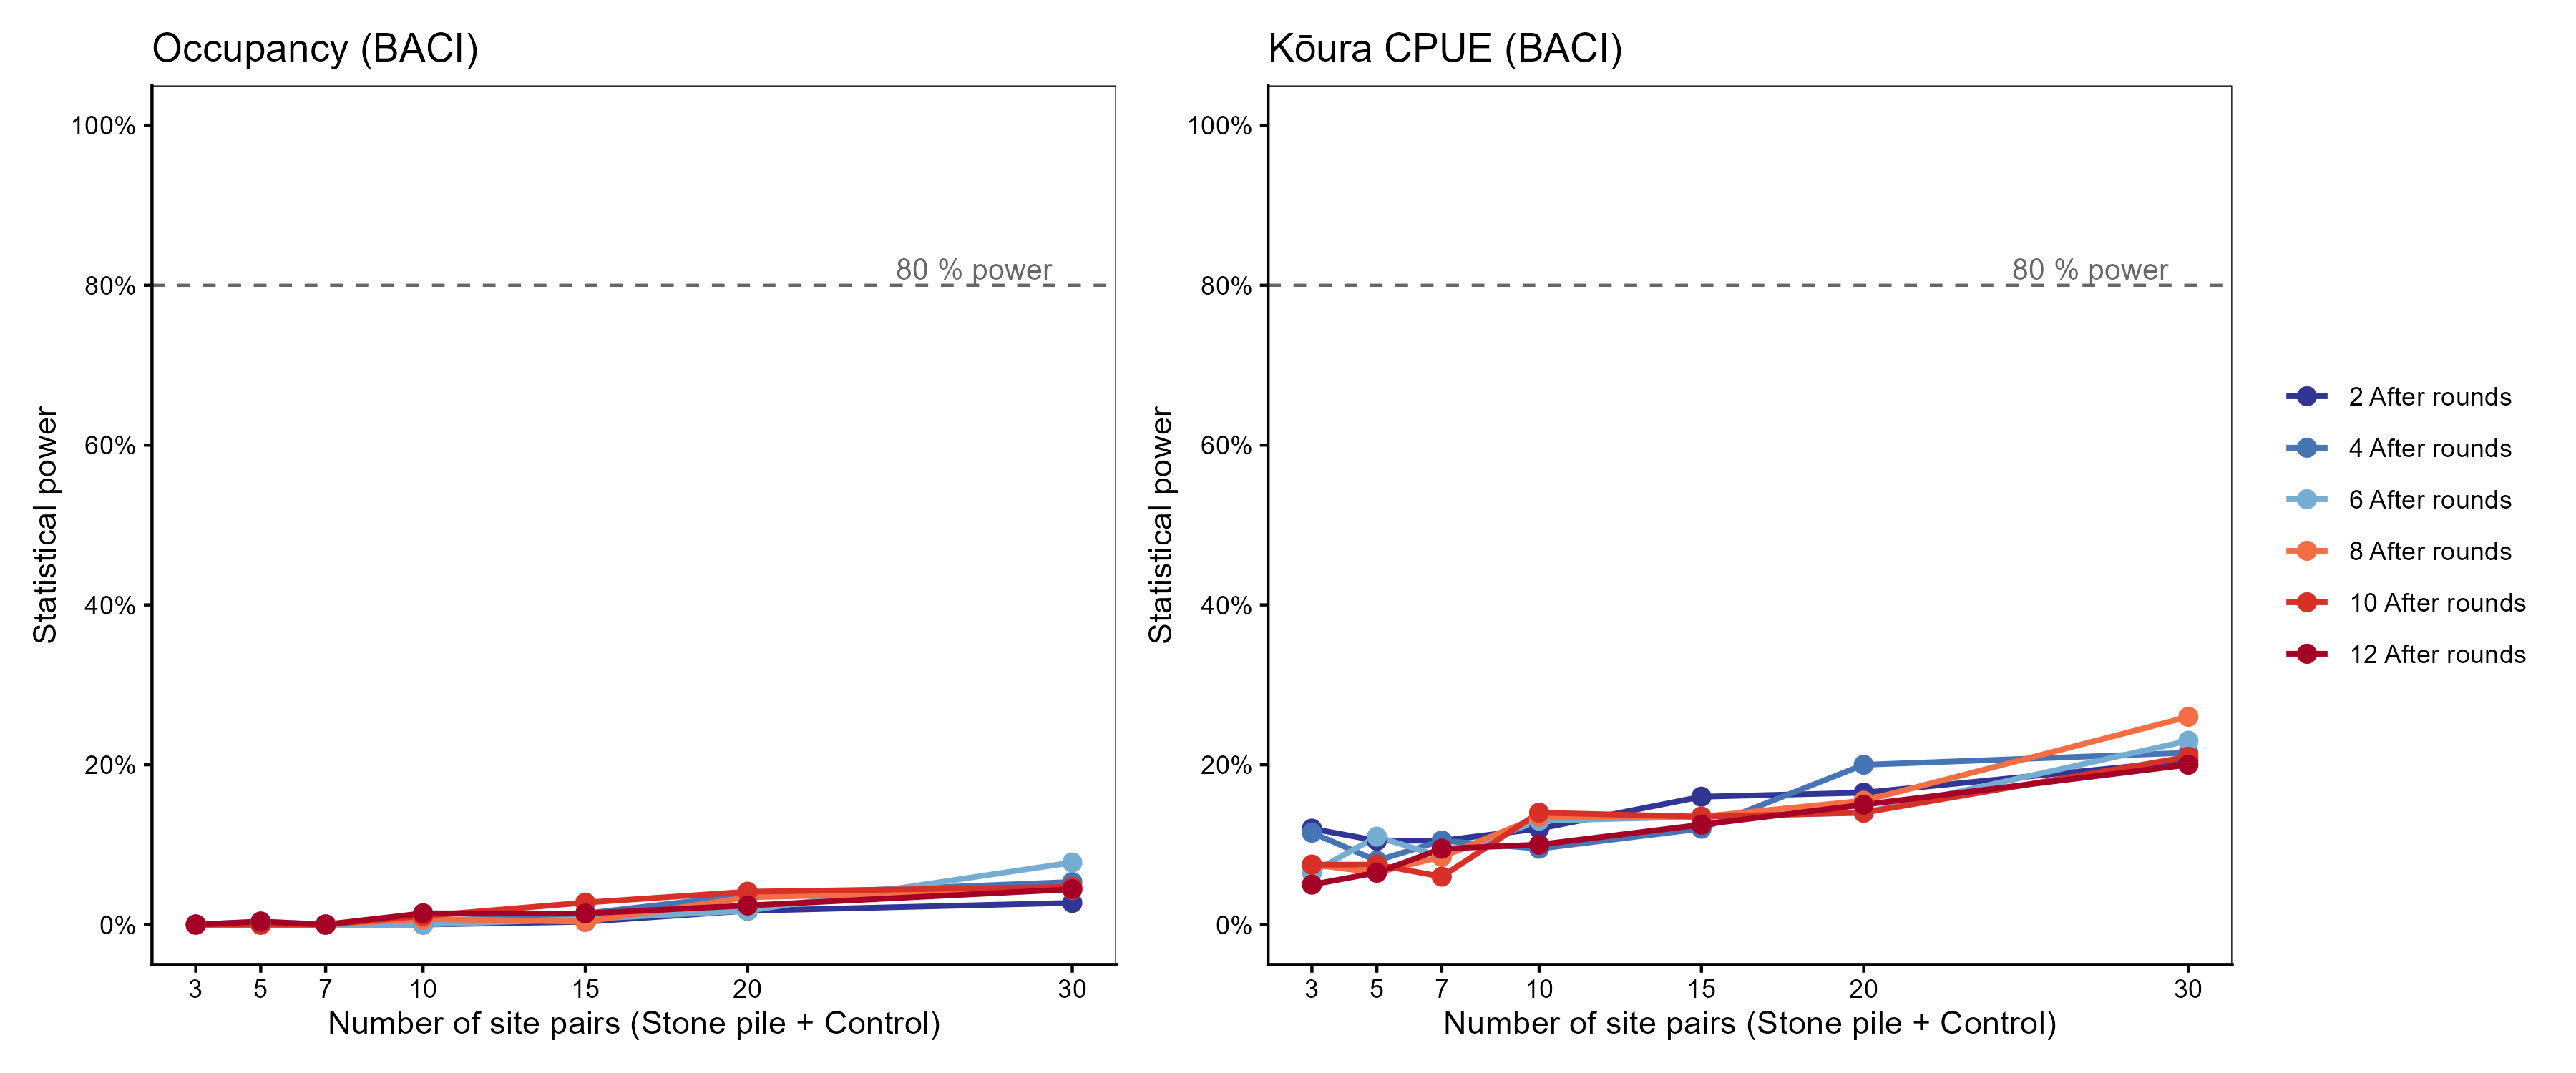
\includegraphics[width=0.8\linewidth,height=\textheight,keepaspectratio]{outputs/fig-power-curves-combined.png}

}

\caption{\label{fig-power-curves-combined}Simulation-based power curves
for the occupancy BACI (left) and kōura CPUE BACI (right). Each line
represents a different number of After-period monitoring rounds. Dashed
line marks 80 \% power.}

\end{figure}%

\begin{figure}

\centering{

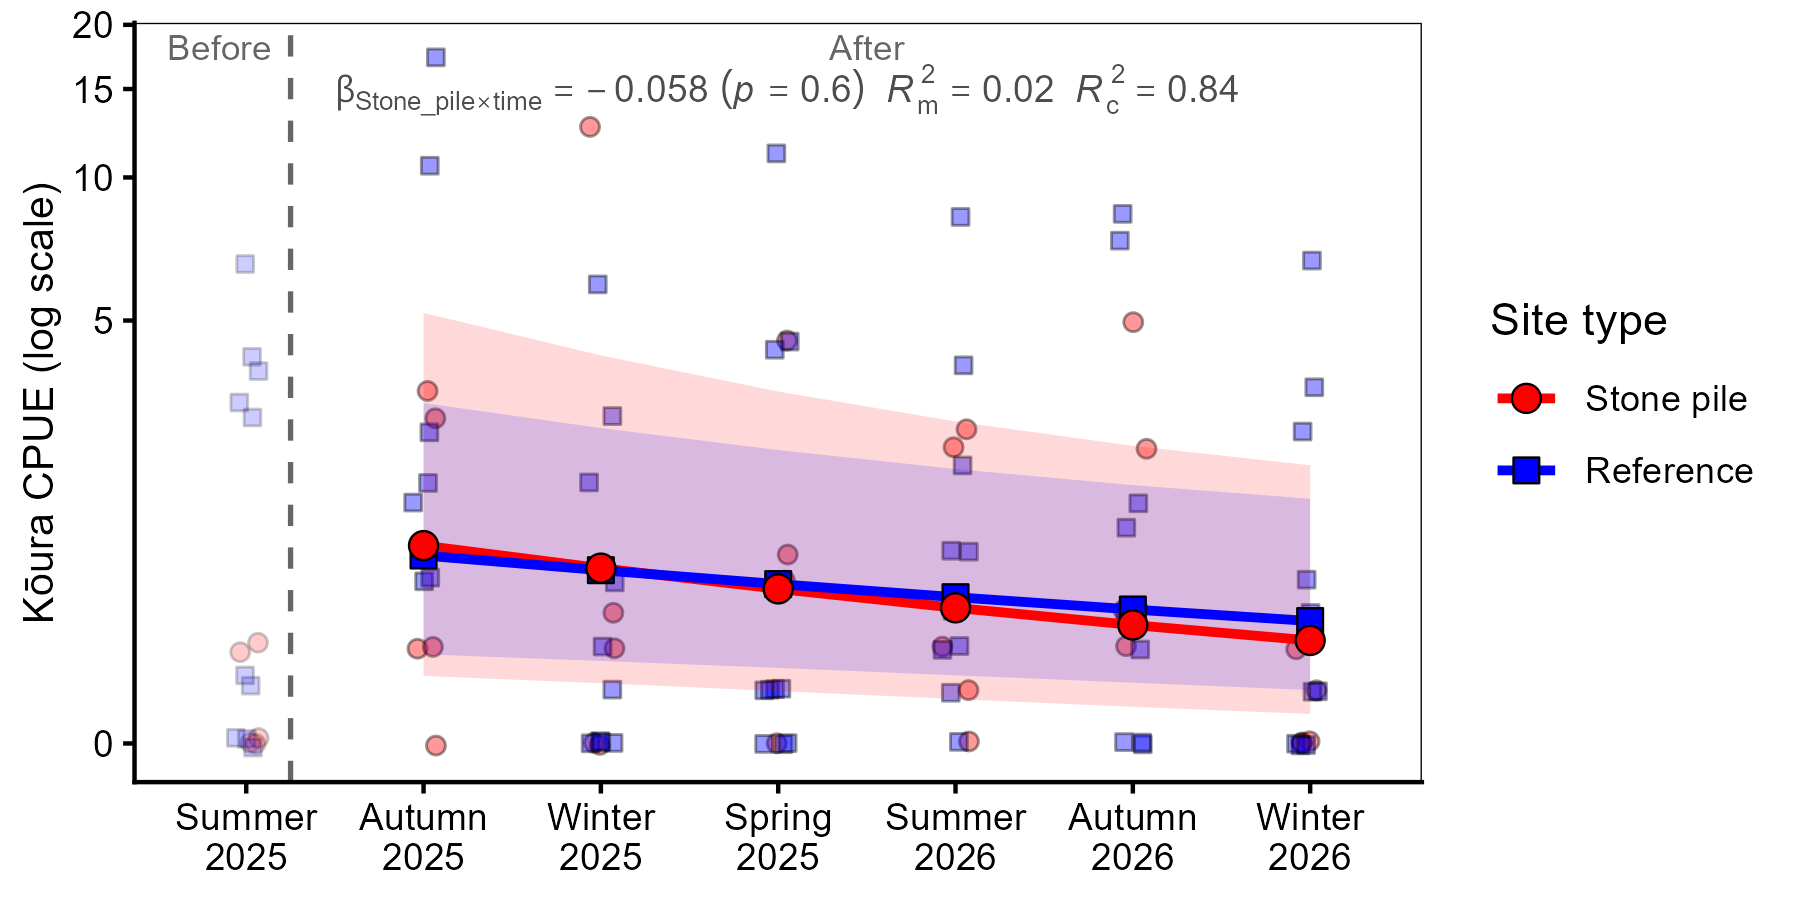
\includegraphics[width=0.8\linewidth,height=\textheight,keepaspectratio]{outputs/fig-convergence-plot.png}

}

\caption{\label{fig-convergence-plot}Predicted kōura CPUE trajectories
over monitoring rounds at stone pile and reference sites from the
abundance convergence model. Shaded ribbons represent 95\% confidence
intervals. The annotation shows the key interaction term (\(\beta\) ±
p-value) and model R² values for fixed effects (R²m) and conditional
(R²c).}

\end{figure}%

\clearpage
\nopagecolor
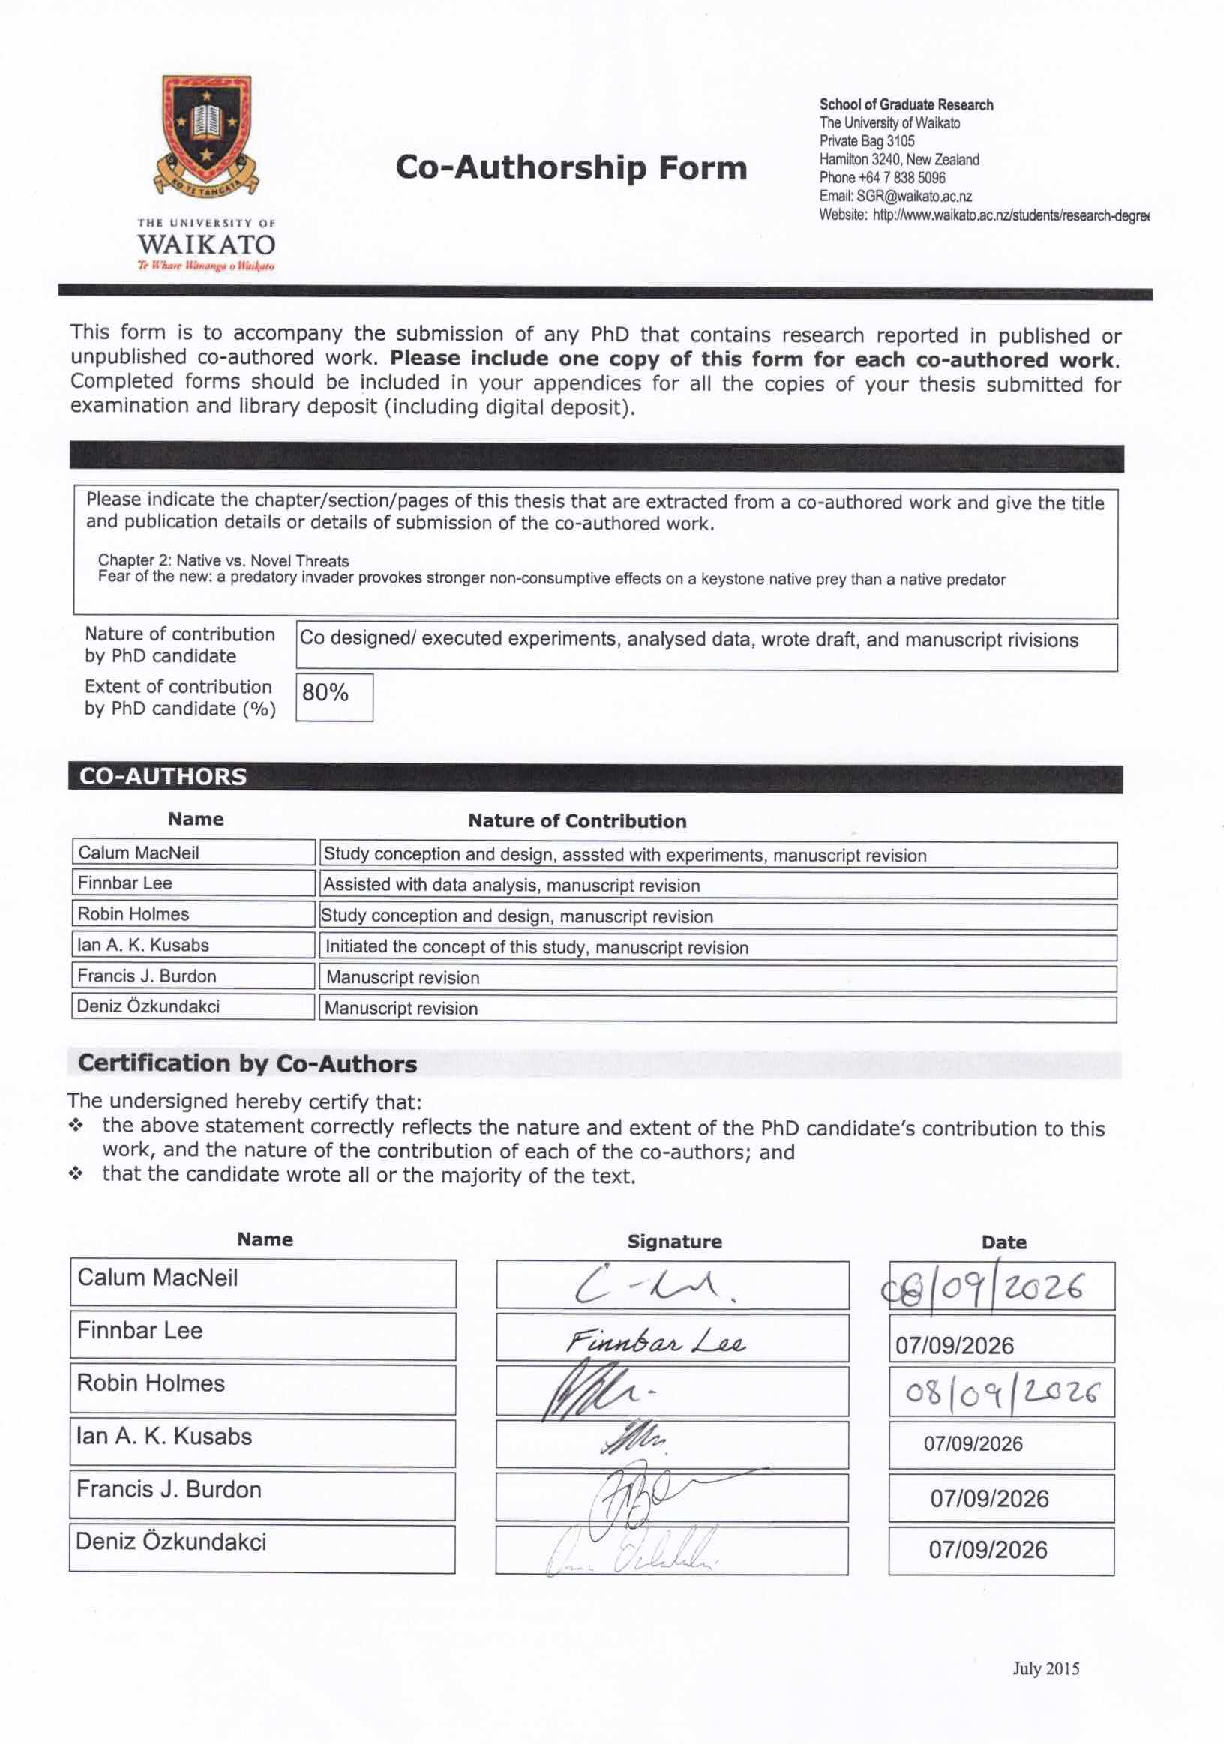
\includepdf[pages=1,pagecommand={}]{admin/Co-Authorship-Form_ch2.pdf}
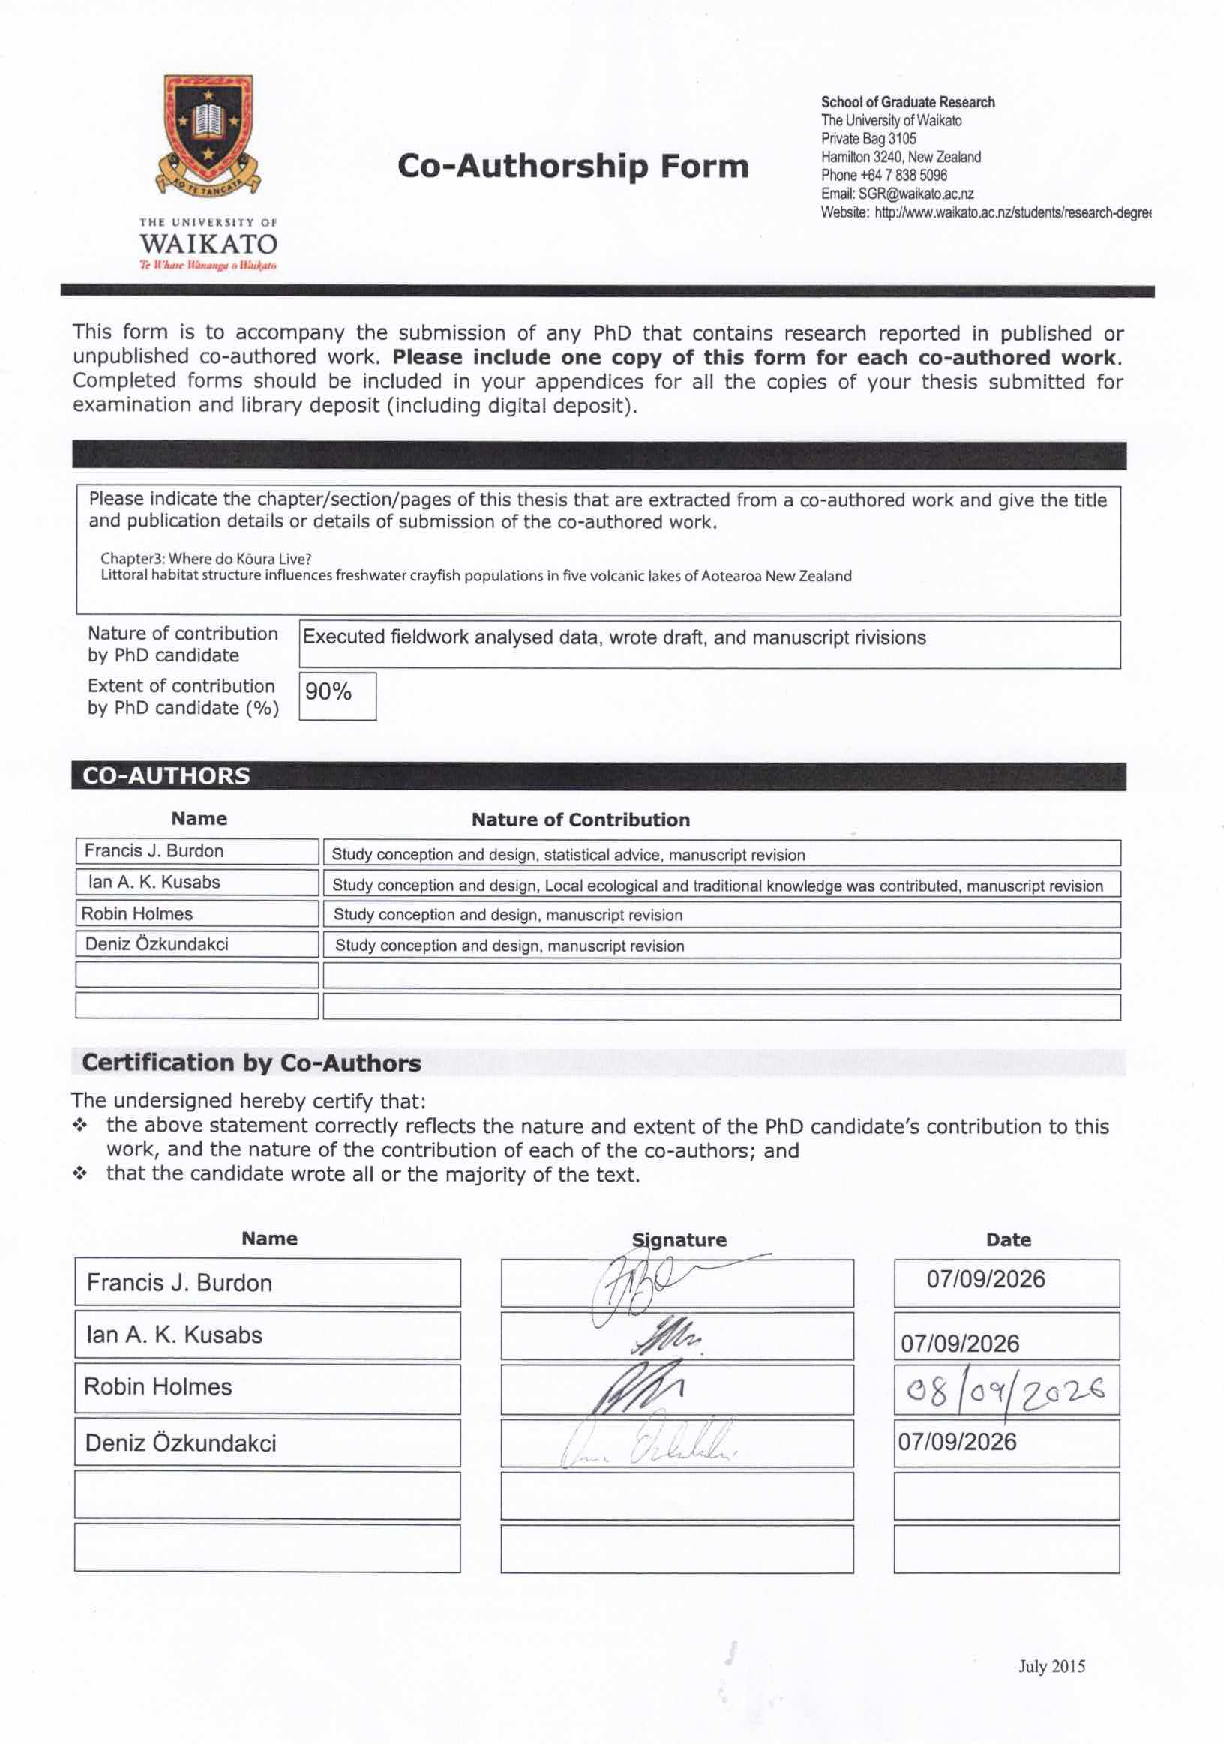
\includepdf[pages=1,pagecommand={}]{admin/Co-Authorship-Form_ch3.pdf}
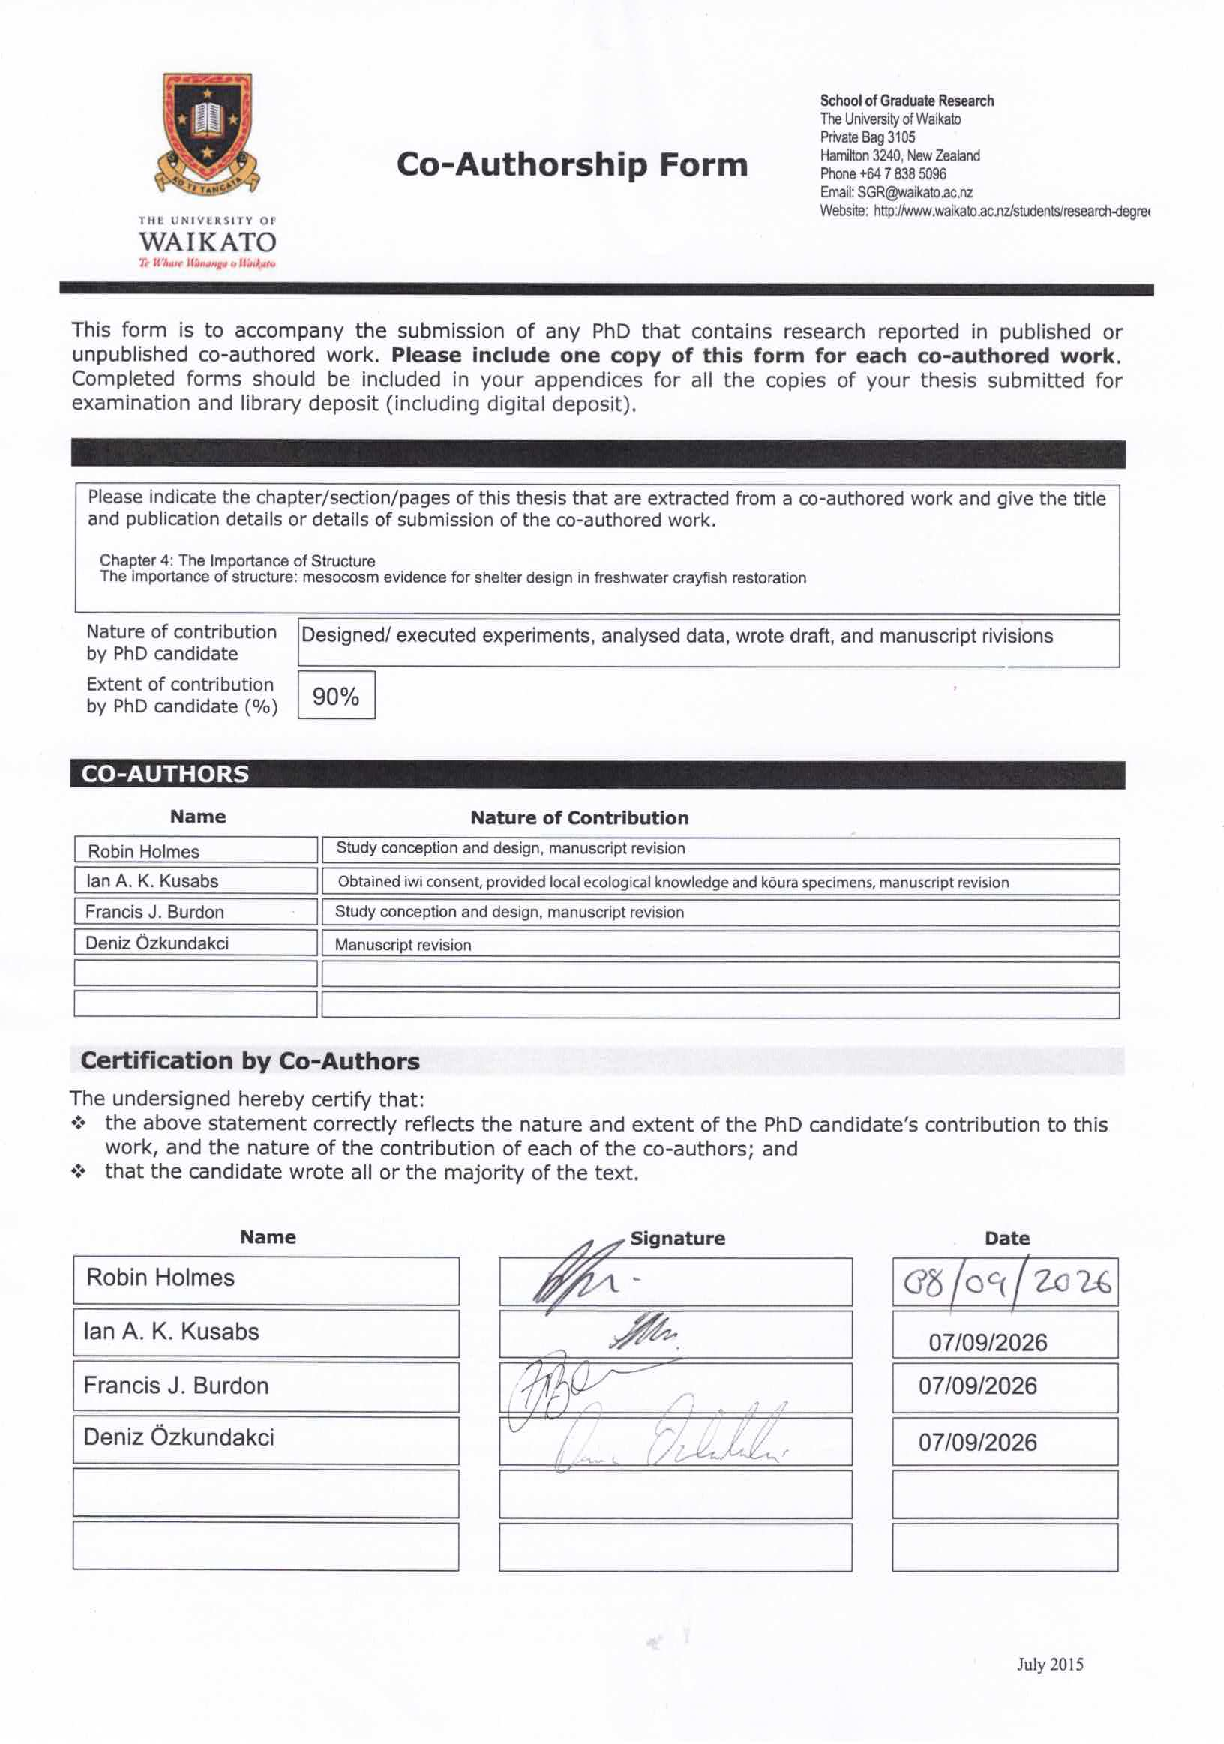
\includepdf[pages=1,pagecommand={}]{admin/Co-Authorship-Form_ch4.pdf}
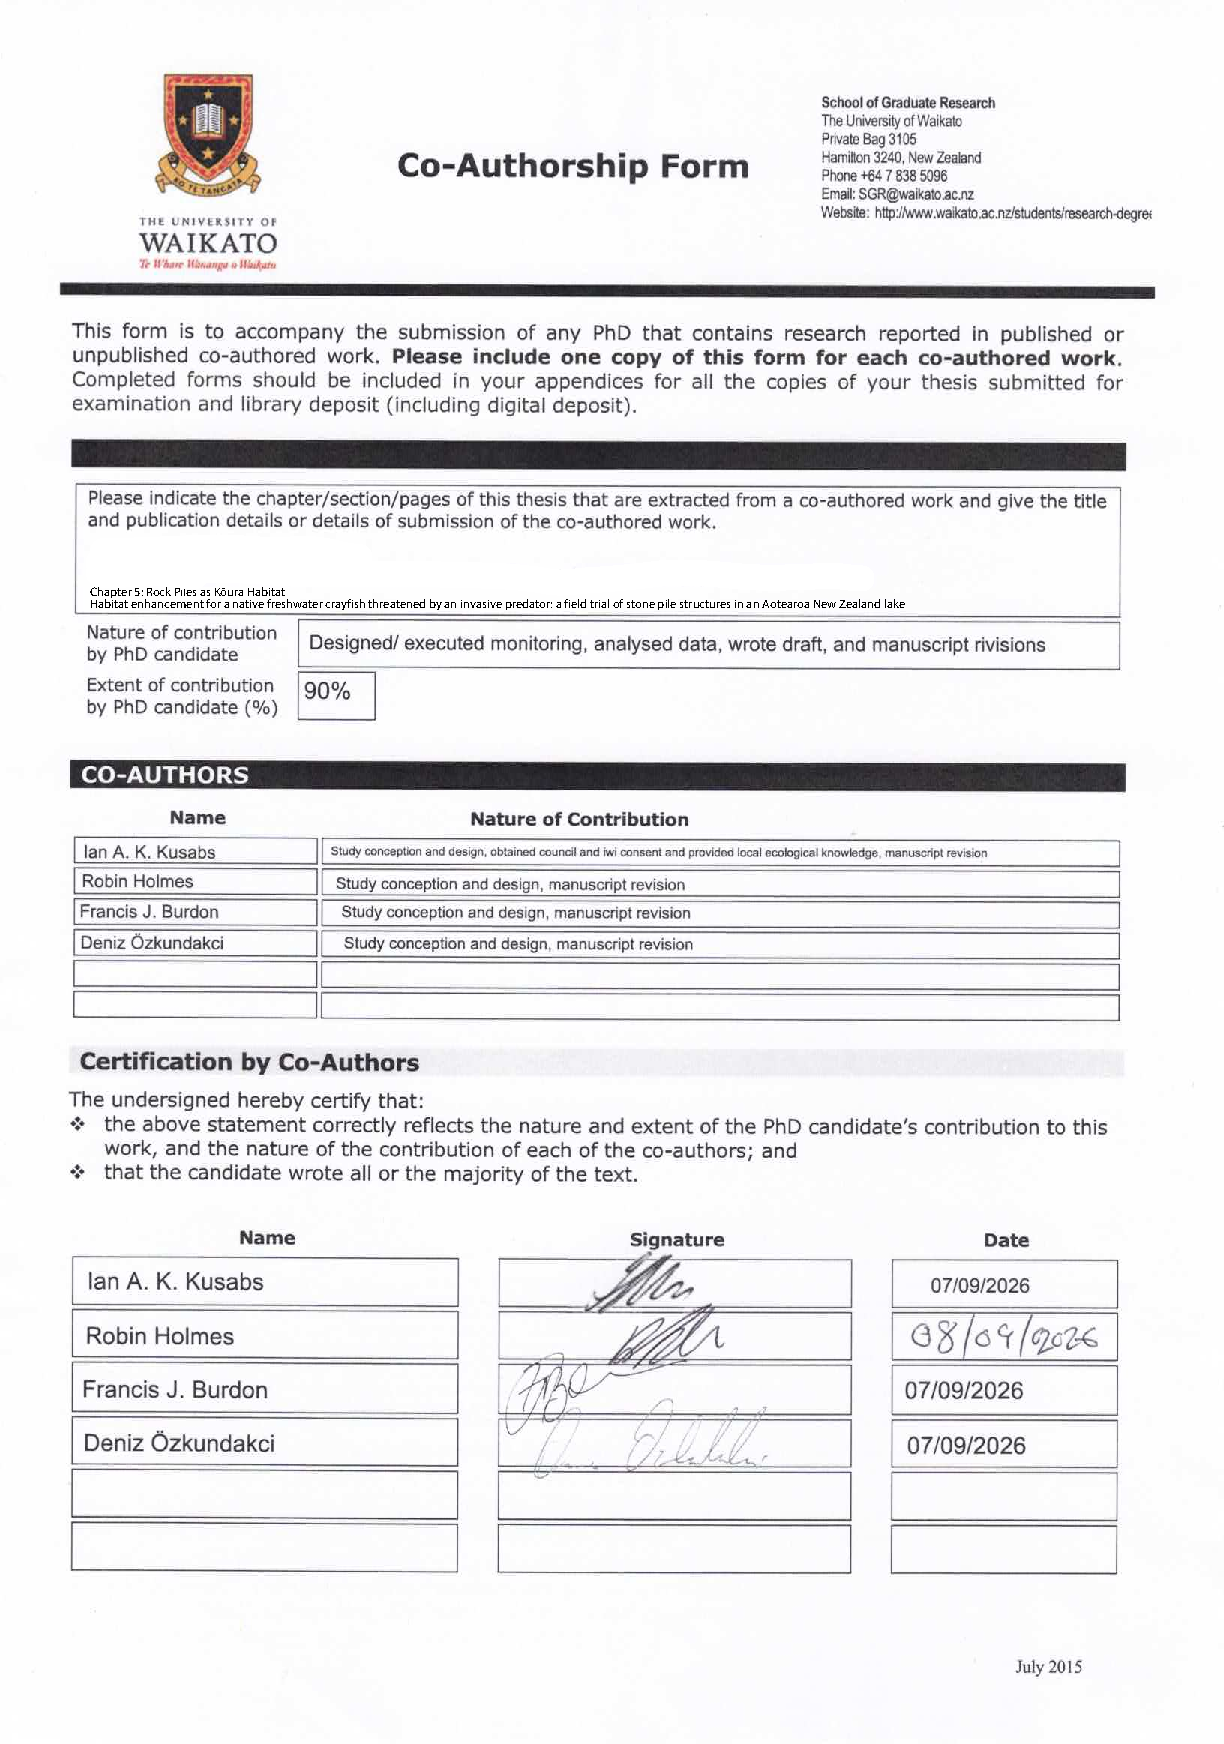
\includepdf[pages=1,pagecommand={}]{admin/Co-Authorship-Form_ch5.pdf}
\clearpage
\pagecolor{thesiscream}

\clearpage
\thispagestyle{empty}
\begin{tikzpicture}[remember picture, overlay]
  \fill[black] (current page.north west) rectangle ([yshift=-6cm]current page.north east);
  \fill[black] ([yshift=8cm]current page.south west) rectangle (current page.south east);
  \begin{scope}
    \clip ([yshift=-6cm]current page.north west)
          rectangle ([yshift=8cm]current page.south east);
    \node[inner sep=0pt, anchor=north]
      at ([yshift=-6cm]current page.north)
      {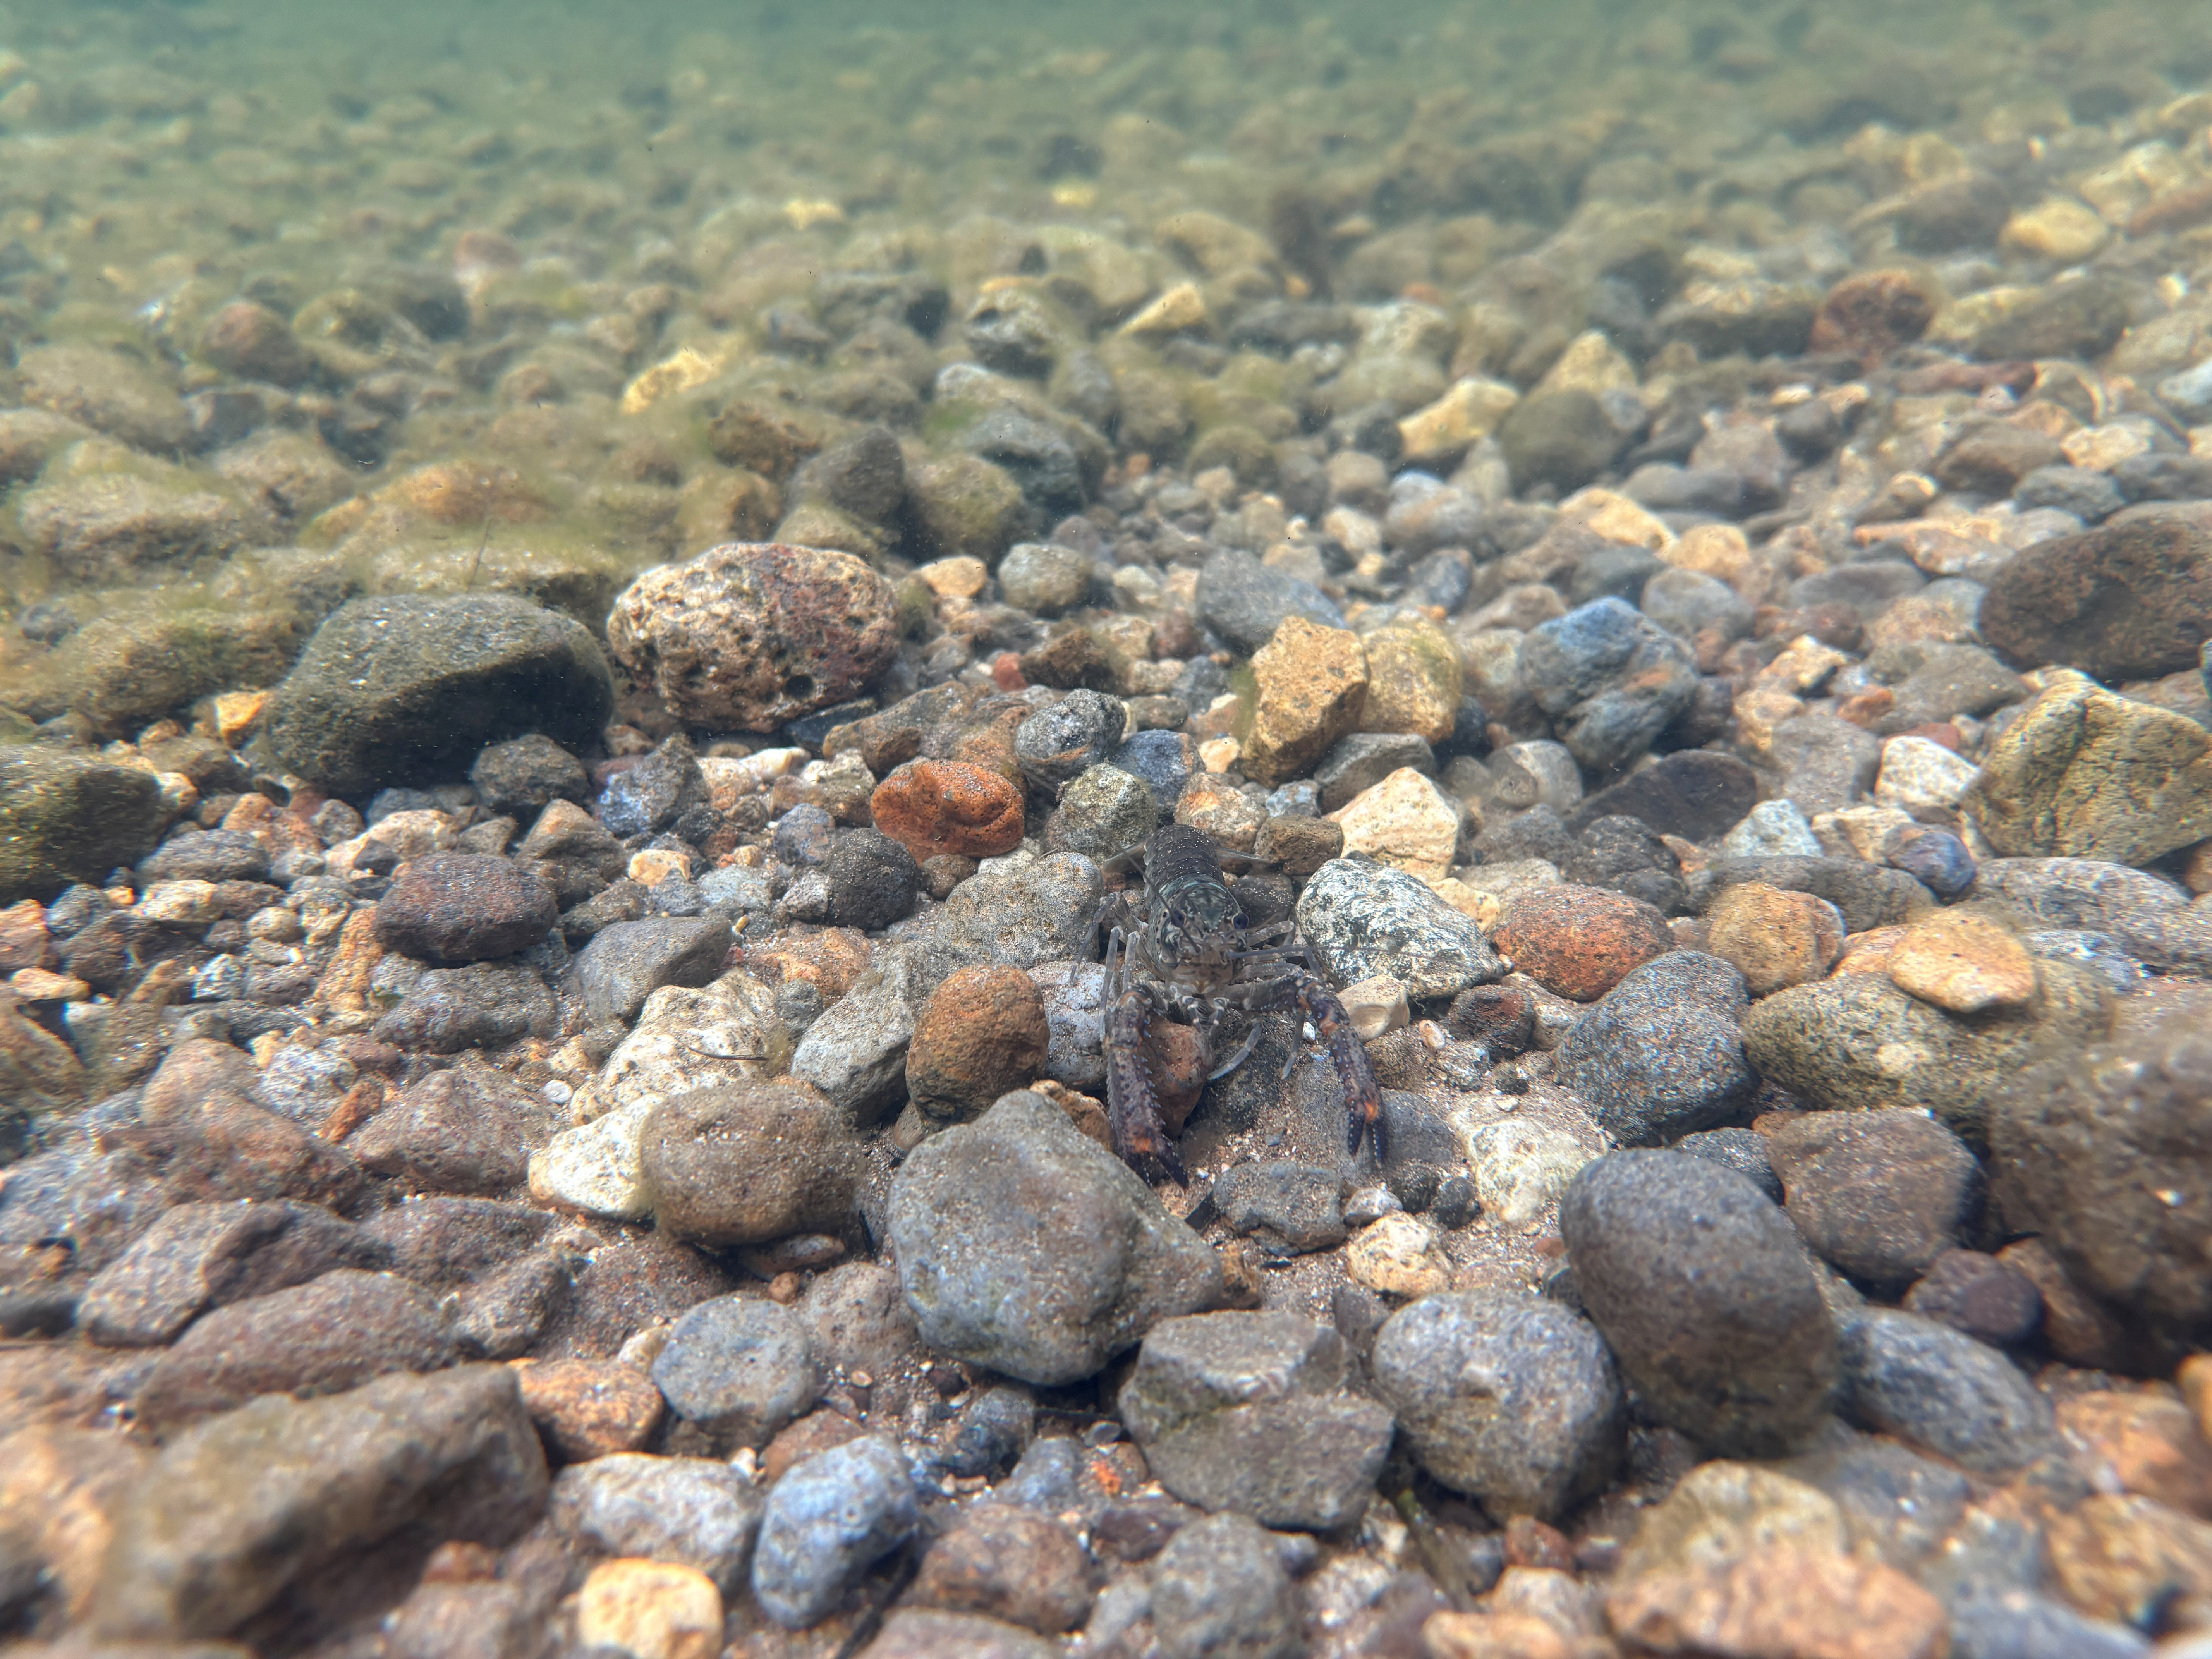
\includegraphics[width=\paperwidth]{images/thesis_back_cover.jpg}};
  \end{scope}
\end{tikzpicture}
\null
\clearpage


\backmatter


\end{document}
